%&preformat-disser
\RequirePackage[l2tabu,orthodox]{nag} % Раскомментировав, можно в логе получать рекомендации относительно правильного использования пакетов и предупреждения об устаревших и нерекомендуемых пакетах
% Формат А4, 14pt (ГОСТ Р 7.0.11-2011, 5.3.6)
\documentclass[a4paper,14pt,oneside,openany]{memoir}

%%%%%%%%%%%%%%%%%%%%%%%%%%%%%%%%%%%%%%%%%%%%%%%%%%%%%%%%%%%%%%%%%%%%%%%%%%%%%%%%
%%%% Файл упрощённых настроек шаблона, общих для диссертации и автореферата %%%%
%%%%%%%%%%%%%%%%%%%%%%%%%%%%%%%%%%%%%%%%%%%%%%%%%%%%%%%%%%%%%%%%%%%%%%%%%%%%%%%%

%%% Режим черновика %%%
\makeatletter
\@ifundefined{c@draft}{
  \newcounter{draft}
  \setcounter{draft}{1}  % 0 --- чистовик (максимальное соблюдение ГОСТ)
                         % 1 --- черновик (отклонения от ГОСТ, но быстрая
                         %       сборка итоговых PDF)
}{}
\makeatother

%%% Пометки в тексте %%%
\makeatletter
\@ifundefined{c@showmarkup}{
  \newcounter{showmarkup}
  \setcounter{showmarkup}{0}  % 0 --- скрыть пометки
                              % 1 --- показывать пометки
}{}
\makeatother

%%% Использование в pdflatex шрифтов не по-умолчанию %%%
\makeatletter
\@ifundefined{c@usealtfont}{
  \newcounter{usealtfont}
  \setcounter{usealtfont}{1}    % 0 --- шрифты на базе Computer Modern
                                % 1 --- использовать пакет pscyr, при его
                                %       наличии
                                % 2 --- использовать пакет XCharter, при наличии
                                %       подходящей версии
}{}
\makeatother

%%% Использование в xelatex и lualatex семейств шрифтов %%%
\makeatletter
\@ifundefined{c@fontfamily}{
  \newcounter{fontfamily}
  \setcounter{fontfamily}{1}  % 0 --- CMU семейство. Используется как fallback;
                              % 1 --- Шрифты от MS (Times New Roman и компания)
                              % 2 --- Семейство Liberation
}{}
\makeatother

%%% Библиография %%%
\makeatletter
\@ifundefined{c@bibliosel}{
  \newcounter{bibliosel}
  \setcounter{bibliosel}{1}   % 0 --- встроенная реализация с загрузкой файла
                              %       через движок bibtex8;
                              % 1 --- реализация пакетом biblatex через движок
                              %       biber
}{}
\makeatother

%%% Вывод типов ссылок в библиографии %%%
\makeatletter
\@ifundefined{c@mediadisplay}{
  \newcounter{mediadisplay}
  \setcounter{mediadisplay}{1}   % 0 --- не делать ничего; надписи [Текст] и
                                 %       [Эл. ресурс] будут выводиться только в ссылках с
                                 %       заполненным полем `media`;
                                 % 1 --- автоматически добавлять надпись [Текст] к ссылкам с
                                 %       незаполненным полем `media`; таким образом, у всех
                                 %       источников будет указан тип, что соответствует
                                 %       требованиям ГОСТ
                                 % 2 --- автоматически удалять надписи [Текст], [Эл. Ресурс] и др.;
                                 %       не соответствует ГОСТ
                                 % 3 --- автоматически удалять надпись [Текст];
                                 %       не соответствует ГОСТ
                                 % 4 --- автоматически удалять надпись [Эл. Ресурс];
                                 %       не соответствует ГОСТ
}{}
\makeatother

%%% Предкомпиляция tikz рисунков для ускорения работы %%%
\makeatletter
\@ifundefined{c@imgprecompile}{
  \newcounter{imgprecompile}
  \setcounter{imgprecompile}{0}   % 0 --- без предкомпиляции;
                                  % 1 --- пользоваться предварительно
                                  %       скомпилированными pdf вместо генерации
                                  %       заново из tikz
}{}
\makeatother
            % общие настройки шаблона
%%% Проверка используемого TeX-движка %%%
\newif\ifxetexorluatex   % определяем новый условный оператор (http://tex.stackexchange.com/a/47579)
\ifxetex
    \xetexorluatextrue
\else
    \ifluatex
        \xetexorluatextrue
    \else
        \xetexorluatexfalse
    \fi
\fi

\newif\ifsynopsis           % Условие, проверяющее, что документ --- автореферат

\usepackage{etoolbox}[2015/08/02]   % Для продвинутой проверки разных условий
\providebool{presentation}

\usepackage{comment}    % Позволяет убирать блоки текста (добавляет
                        % окружение comment и команду \excludecomment)

%%% Поля и разметка страницы %%%
\usepackage{pdflscape}  % Для включения альбомных страниц
\usepackage{geometry}   % Для последующего задания полей

%%% Математические пакеты %%%
\usepackage{amsthm,amsmath,amscd}   % Математические дополнения от AMS
\usepackage{amsfonts,amssymb}       % Математические дополнения от AMS
\usepackage{mathtools}              % Добавляет окружение multlined
\usepackage{xfrac}                  % Красивые дроби
\usepackage[
    locale = DE,
    list-separator       = {;\,},
    list-final-separator = {;\,},
    list-pair-separator  = {;\,},
    list-units           = single,
    range-units          = single,
    range-phrase={\text{\ensuremath{-}}},
    % quotient-mode        = fraction, % красивые дроби могут не соответствовать ГОСТ
    fraction-function    = \sfrac,
    separate-uncertainty,
    ]{siunitx}[=v2]                 % Размерности SI
\sisetup{inter-unit-product = \ensuremath{{}\cdot{}}}

% Кириллица в нумерации subequations
% Для правильной работы требуется выполнение сразу после загрузки пакетов
\patchcmd{\subequations}{\def\theequation{\theparentequation\alph{equation}}}
{\def\theequation{\theparentequation\asbuk{equation}}}
{\typeout{subequations patched}}{\typeout{subequations not patched}}

%%%% Установки для размера шрифта 14 pt %%%%
%% Формирование переменных и констант для сравнения (один раз для всех подключаемых файлов)%%
%% должно располагаться до вызова пакета fontspec или polyglossia, потому что они сбивают его работу
\newlength{\curtextsize}
\newlength{\bigtextsize}
\setlength{\bigtextsize}{13.9pt}

\makeatletter
%\show\f@size    % неплохо для отслеживания, но вызывает стопорение процесса,
                 % если документ компилируется без команды  -interaction=nonstopmode
\setlength{\curtextsize}{\f@size pt}
\makeatother

%%% Кодировки и шрифты %%%
\ifxetexorluatex
    \ifpresentation
        \providecommand*\autodot{} % quick fix for polyglossia 1.50
    \fi
    \PassOptionsToPackage{no-math}{fontspec}    % https://tex.stackexchange.com/a/26295/104425
    \usepackage{polyglossia}[2014/05/21]        % Поддержка многоязычности
                                        % (fontspec подгружается автоматически)
\else
   %%% Решение проблемы копирования текста в буфер кракозябрами
    \ifnumequal{\value{usealtfont}}{0}{}{
        \input glyphtounicode.tex
        \input glyphtounicode-cmr.tex %from pdfx package
        \pdfgentounicode=1
    }
    \usepackage{cmap}   % Улучшенный поиск русских слов в полученном pdf-файле
    \ifnumequal{\value{usealtfont}}{2}{}{
        \defaulthyphenchar=127  % Если стоит до fontenc, то переносы
                                % не впишутся в выделяемый текст при
                                % копировании его в буфер обмена
    }
    \usepackage{textcomp}
    \usepackage[T1,T2A]{fontenc}                    % Поддержка русских букв
    \ifnumequal{\value{usealtfont}}{1}{% Используется pscyr, при наличии
        \IfFileExists{pscyr.sty}{\usepackage{pscyr}}{}  % Подключение pscyr
    }{}
    \usepackage[utf8]{inputenc}[2014/04/30]         % Кодировка utf8
    \usepackage[english, russian]{babel}[2014/03/24]% Языки: русский, английский
    \makeatletter\AtBeginDocument{\let\@elt\relax}\makeatother % babel 3.40 fix
    \ifnumequal{\value{usealtfont}}{2}{
        % http://dxdy.ru/post1238763.html#p1238763
        \usepackage[scaled=0.914]{XCharter}[2017/12/19] % Подключение русифицированных шрифтов XCharter
        \usepackage[charter, vvarbb, scaled=1.048]{newtxmath}[2017/12/14]
        \ifpresentation
        \else
            \setDisplayskipStretch{-0.078}
        \fi
    }{}
\fi

%%% Оформление абзацев %%%
\ifpresentation
\else
    \indentafterchapter     % Красная строка после заголовков типа chapter
    \usepackage{indentfirst}
\fi

%%% Цвета %%%
\ifpresentation
\else
    \usepackage[dvipsnames, table, hyperref]{xcolor} % Совместимо с tikz
\fi

%%% Таблицы %%%
\usepackage{longtable} % Длинные таблицы
\usepackage{multirow,makecell}   % Улучшенное форматирование таблиц
\usepackage{tabulary,tabularray} % Таблицы с автоматически подбирающейся
                                 % шириной столбцов
\UseTblrLibrary{booktabs}
\ExplSyntaxOn% define \IfTokenListEmpty to use \captionof with tabularray
\prg_generate_conditional_variant:Nnn \tl_if_empty:n { e } { TF }
\let \IfTokenListEmpty = \tl_if_empty:eTF
\ExplSyntaxOff

\usepackage{threeparttable}      % автоматический подгон ширины подписи таблицы

%%% Общее форматирование
%\usepackage{soul}% Поддержка переносоустойчивых подчёркиваний и зачёркиваний
\usepackage{icomma}  % Запятая в десятичных дробях

%%% Оптимизация расстановки переносов и длины последней строки абзаца
\IfFileExists{impnattypo.sty}{% проверка установленности пакета impnattypo
    \ifluatex
        \ifnumequal{\value{draft}}{1}{% Черновик
            \usepackage[hyphenation, lastparline, nosingleletter, homeoarchy,
            rivers, draft]{impnattypo}
        }{% Чистовик
            \usepackage[hyphenation, lastparline, nosingleletter]{impnattypo}
        }
    \else
        \usepackage[hyphenation, lastparline]{impnattypo}
    \fi
}{}

%% Векторная графика

\usepackage{tikz}                   % Продвинутый пакет векторной графики
\usetikzlibrary{chains}             % Для примера tikz рисунка
\usetikzlibrary{shapes.geometric}   % Для примера tikz рисунка
\usetikzlibrary{shapes.symbols}     % Для примера tikz рисунка
\usetikzlibrary{arrows}             % Для примера tikz рисунка

\usepackage[european,cuteinductors]{circuitikz} % Электрические схемы
\usepackage{pgfplots}                           % Графики
\pgfplotsset{compat=newest}
\usepgfplotslibrary{groupplots,units}
\pgfkeys{/pgf/number format/.cd,use comma,1000 sep={}} % форматирование чисел в графиках

%%% Гиперссылки %%%
\ifxetexorluatex
    \let\CYRDZE\relax
\fi
\usepackage{hyperref}[2012/11/06]

%%% Изображения %%%
\usepackage{graphicx}[2014/04/25]   % Подключаем пакет работы с графикой
\usepackage{caption}                % Подписи рисунков и таблиц
\usepackage{subcaption}             % Подписи подрисунков и подтаблиц
\usepackage{pdfpages}               % Добавление внешних pdf файлов

%%% Счётчики %%%
\usepackage{aliascnt}
\usepackage[figure,table]{totalcount}   % Счётчик рисунков и таблиц
\usepackage{totcount}   % Пакет создания счётчиков на основе последнего номера
                        % подсчитываемого элемента (может требовать дважды
                        % компилировать документ)
\usepackage{totpages}   % Счётчик страниц, совместимый с hyperref (ссылается
                        % на номер последней страницы). Желательно ставить
                        % последним пакетом в преамбуле

%%% Продвинутое управление групповыми ссылками (пока только формулами) %%%
\ifpresentation
\else
    \usepackage[russian]{cleveref} % cleveref имеет сложности со считыванием
    % языка из babel. Такое решение русификации вывода выбрано вместо
    % определения в documentclass из опасности что-то лишнее передать во все
    % остальные пакеты, включая библиографию.

    % Добавление возможности использования пробелов в \labelcref
    % https://tex.stackexchange.com/a/340502/104425
    \usepackage{kvsetkeys}
    \makeatletter
    \let\org@@cref\@cref
    \renewcommand*{\@cref}[2]{%
        \edef\process@me{%
            \noexpand\org@@cref{#1}{\zap@space#2 \@empty}%
        }\process@me
    }
    \makeatother
\fi

\usepackage{placeins} % для \FloatBarrier

\ifnumequal{\value{draft}}{1}{% Черновик
    \usepackage[firstpage]{draftwatermark}
    \SetWatermarkText{DRAFT}
    \SetWatermarkFontSize{14pt}
    \SetWatermarkScale{15}
    \SetWatermarkAngle{45}
}{}

%%% Цитата, не приводимая в автореферате:
% возможно, актуальна только для biblatex
%\newcommand{\citeinsynopsis}[1]{\ifsynopsis\else ~\cite{#1} \fi}

% если текущий процесс запущен библиотекой tikz-external, то прекомпиляция должна быть включена
\ifdefined\tikzexternalrealjob
    \setcounter{imgprecompile}{1}
\fi

\ifnumequal{\value{imgprecompile}}{1}{% Только если у нас включена предкомпиляция
    \usetikzlibrary{external}   % подключение возможности предкомпиляции
    \tikzexternalize[prefix=images/cache/,optimize command away=\includepdf] % activate! % здесь можно указать отдельную папку для скомпилированных файлов
    \ifxetex
        \tikzset{external/up to date check={diff}}
    \fi
}{}
         % Пакеты общие для диссертации и автореферата
\synopsisfalse                      % Этот документ --- не автореферат
%%% Прикладные пакеты %%%
%\usepackage{calc}               % Пакет для расчётов параметров, например длины

%%% Для добавления Стр. над номерами страниц в оглавлении
%%% http://tex.stackexchange.com/a/306950
\usepackage{afterpage}

%%% Списки %%%
\usepackage{enumitem}

%%% Оформление списка обозначений
\usepackage[intoc]{nomencl}
\makenomenclature
\setlength{\nomitemsep}{-.8\parsep}
    % Пакеты для диссертации
\usepackage{fr-longtable}    %ради \endlasthead

% Листинги с исходным кодом программ
\usepackage{fancyvrb}
\usepackage{listings}
\lccode`\~=0\relax %Без этого хака из-за особенностей пакета listings перестают работать конструкции с \MakeLowercase и т. п. в (xe|lua)latex

% Русская традиция начертания греческих букв
\usepackage{upgreek} % прямые греческие ради русской традиции

%%% Микротипографика
%\ifnumequal{\value{draft}}{0}{% Только если у нас режим чистовика
%    \usepackage[final, babel, shrink=45]{microtype}[2016/05/14] % улучшает представление букв и слов в строках, может помочь при наличии отдельно висящих слов
%}{}

% Отметка о версии черновика на каждой странице
% Чтобы работало надо в своей локальной копии по инструкции
% https://www.ctan.org/pkg/gitinfo2 создать небходимые файлы в папке
% ./git/hooks
% If you’re familiar with tweaking git, you can probably work it out for
% yourself. If not, I suggest you follow these steps:
% 1. First, you need a git repository and working tree. For this example,
% let’s suppose that the root of the working tree is in ~/compsci
% 2. Copy the file post-xxx-sample.txt (which is in the same folder of
% your TEX distribution as this pdf) into the git hooks directory in your
% working copy. In our example case, you should end up with a file called
% ~/compsci/.git/hooks/post-checkout
% 3. If you’re using a unix-like system, don’t forget to make the file executable.
% Just how you do this is outside the scope of this manual, but one
% possible way is with commands such as this:
% chmod g+x post-checkout.
% 4. Test your setup with “git checkout master” (or another suitable branch
% name). This should generate copies of gitHeadInfo.gin in the directories
% you intended.
% 5. Now make two more copies of this file in the same directory (hooks),
% calling them post-commit and post-merge, and you’re done. As before,
% users of unix-like systems should ensure these files are marked as
% executable.
\ifnumequal{\value{draft}}{1}{% Черновик
   \IfFileExists{.git/gitHeadInfo.gin}{
      \usepackage[mark,pcount]{gitinfo2}
      \renewcommand{\gitMark}{rev.\gitAbbrevHash\quad\gitCommitterEmail\quad\gitAuthorIsoDate}
      \renewcommand{\gitMarkFormat}{\rmfamily\color{Gray}\small\bfseries}
   }{}
}{}   % Пакеты для специфических пользовательских задач


\usepackage{svg}
\usepackage{amsmath}
\usepackage{pgfplots}
\pgfplotsset{compat=1.17}
\usepackage{tikz}
\usetikzlibrary{intersections}
\usetikzlibrary{calc, positioning, shapes, shapes.callouts, arrows.meta, shapes.geometric, plotmarks, matrix, backgrounds}
\usepackage{pgfplots}
\pgfplotsset{compat=newest}
\usepgfplotslibrary{fillbetween}
\usepackage{fullwidth}
\usepackage{xcolor}


%%%%%%%%%%%%%%%%%%%%%%%%%%%%%%%%%%%%%%%%%%%%%%%%%%%%%%
%%%% Файл упрощённых настроек шаблона диссертации %%%%
%%%%%%%%%%%%%%%%%%%%%%%%%%%%%%%%%%%%%%%%%%%%%%%%%%%%%%

%%% Инициализирование переменных, не трогать!  %%%
\newcounter{intvl}
\newcounter{otstup}
\newcounter{contnumeq}
\newcounter{contnumfig}
\newcounter{contnumtab}
\newcounter{pgnum}
\newcounter{chapstyle}
\newcounter{headingdelim}
\newcounter{headingalign}
\newcounter{headingsize}
%%%%%%%%%%%%%%%%%%%%%%%%%%%%%%%%%%%%%%%%%%%%%%%%%%%%%%

%%% Область упрощённого управления оформлением %%%

%% Интервал между заголовками и между заголовком и текстом %%
% Заголовки отделяют от текста сверху и снизу
% тремя интервалами (ГОСТ Р 7.0.11-2011, 5.3.5)
\setcounter{intvl}{3}               % Коэффициент кратности к размеру шрифта

%% Отступы у заголовков в тексте %%
\setcounter{otstup}{0}              % 0 --- без отступа; 1 --- абзацный отступ

%% Нумерация формул, таблиц и рисунков %%
% Нумерация формул
\setcounter{contnumeq}{0}   % 0 --- пораздельно (во введении подряд,
                            %       без номера раздела);
                            % 1 --- сквозная нумерация по всей диссертации
% Нумерация рисунков
\setcounter{contnumfig}{0}  % 0 --- пораздельно (во введении подряд,
                            %       без номера раздела);
                            % 1 --- сквозная нумерация по всей диссертации
% Нумерация таблиц
\setcounter{contnumtab}{1}  % 0 --- пораздельно (во введении подряд,
                            %       без номера раздела);
                            % 1 --- сквозная нумерация по всей диссертации

%% Оглавление %%
\setcounter{pgnum}{1}       % 0 --- номера страниц никак не обозначены;
                            % 1 --- Стр. над номерами страниц (дважды
                            %       компилировать после изменения настройки)
\settocdepth{subsection}    % до какого уровня подразделов выносить в оглавление
\setsecnumdepth{subsection} % до какого уровня нумеровать подразделы


%% Текст и форматирование заголовков %%
\setcounter{chapstyle}{1}     % 0 --- разделы только под номером;
                              % 1 --- разделы с названием "Глава" перед номером
\setcounter{headingdelim}{1}  % 0 --- номер отделен пропуском в 1em или \quad;
                              % 1 --- номера разделов и приложений отделены
                              %       точкой с пробелом, подразделы пропуском
                              %       без точки;
                              % 2 --- номера разделов, подразделов и приложений
                              %       отделены точкой с пробелом.

%% Выравнивание заголовков в тексте %%
\setcounter{headingalign}{0}  % 0 --- по центру;
                              % 1 --- по левому краю

%% Размеры заголовков в тексте %%
\setcounter{headingsize}{0}   % 0 --- по ГОСТ, все всегда 14 пт;
                              % 1 --- пропорционально изменяющийся размер
                              %       в зависимости от базового шрифта

%% Подпись таблиц %%

% Смещение строк подписи после первой строки
\newcommand{\tabindent}{0cm}

% Тип форматирования заголовка таблицы:
% plain --- название и текст в одной строке
% split --- название и текст в разных строках
\newcommand{\tabformat}{plain}

%%% Настройки форматирования таблицы `plain`

% Выравнивание по центру подписи, состоящей из одной строки:
% true  --- выравнивать
% false --- не выравнивать
\newcommand{\tabsinglecenter}{false}

% Выравнивание подписи таблиц:
% justified   --- выравнивать как обычный текст («по ширине»)
% centering   --- выравнивать по центру
% centerlast  --- выравнивать по центру только последнюю строку
% centerfirst --- выравнивать по центру только первую строку (не рекомендуется)
% raggedleft  --- выравнивать по правому краю
% raggedright --- выравнивать по левому краю
\newcommand{\tabjust}{justified}

% Разделитель записи «Таблица #» и названия таблицы
\newcommand{\tablabelsep}{~\cyrdash\ }

%%% Настройки форматирования таблицы `split`

% Положение названия таблицы:
% \centering   --- выравнивать по центру
% \raggedleft  --- выравнивать по правому краю
% \raggedright --- выравнивать по левому краю
\newcommand{\splitformatlabel}{\raggedleft}

% Положение текста подписи:
% \centering   --- выравнивать по центру
% \raggedleft  --- выравнивать по правому краю
% \raggedright --- выравнивать по левому краю
\newcommand{\splitformattext}{\raggedright}

%% Подпись рисунков %%
%Разделитель записи «Рисунок #» и названия рисунка
\newcommand{\figlabelsep}{~\cyrdash\ }  % (ГОСТ 2.105, 4.3.1)
                                        % "--- здесь не работает

%%% Цвета гиперссылок %%%
% Latex color definitions: http://latexcolor.com/
\definecolor{linkcolor}{rgb}{0.9,0,0}
\definecolor{citecolor}{rgb}{0,0.6,0}
\definecolor{urlcolor}{rgb}{0,0,1}
%\definecolor{linkcolor}{rgb}{0,0,0} %black
%\definecolor{citecolor}{rgb}{0,0,0} %black
%\definecolor{urlcolor}{rgb}{0,0,0} %black
      % Упрощённые настройки шаблона
% Новые переменные, которые могут использоваться во всём проекте
% ГОСТ 7.0.11-2011
% 9.2 Оформление текста автореферата диссертации
% 9.2.1 Общая характеристика работы включает в себя следующие основные структурные
% элементы:
% актуальность темы исследования;
\newcommand{\actualityTXT}{Актуальность темы.}
% степень ее разработанности;
\newcommand{\progressTXT}{Степень разработанности темы.}
% цели и задачи;
\newcommand{\aimTXT}{Целью}
\newcommand{\tasksTXT}{задачи}
% Объект и субъект исследования
\newcommand{\researchObjectTXT}{Объектом исследования}
\newcommand{\researchSubjectTXT}{Предметом исследования}
% научную новизну;
\newcommand{\noveltyTXT}{Научная новизна:}
% научную новизну;
\newcommand{\theoreticalValueTXT}{Теоретическая значимость}
\newcommand{\practicalValueTXT}{Практическая значимость:}
% теоретическую и практическую значимость работы;
%\newcommand{\influenceTXT}{Теоретическая и практическая значимость}
% или чаще используют просто
\newcommand{\influenceTXT}{Практическая значимость}
% методологию и методы исследования;
\newcommand{\methodsTXT}{Методология и методы исследования.}
% положения, выносимые на защиту;
\newcommand{\defpositionsTXT}{Основные положения, выносимые на~защиту:}
% положения, выносимые на защиту;
\newcommand{\specialityRelationTXT}{Область исследования.}
% степень достоверности и апробацию результатов.
\newcommand{\reliabilityTXT}{Достоверность}
\newcommand{\probationTXT}{Апробация работы.}

\newcommand{\contributionTXT}{Личный вклад.}
\newcommand{\publicationsTXT}{Публикации.}


%%% Заголовки библиографии:

% для автореферата:
\newcommand{\bibtitleauthor}{ОСНОВНЫЕ ПУБЛИКАЦИИ ПО ТЕМЕ ДИССЕРТАЦИИ}

% для стиля библиографии `\insertbiblioauthorgrouped`
\newcommand{\bibtitleauthorvak}{В изданиях из списка ВАК РФ}
\newcommand{\bibtitleauthorscopus}{В изданиях, входящих в международную базу цитирования Scopus}
\newcommand{\bibtitleauthorwos}{В изданиях, входящих в международную базу цитирования Web of Science}
\newcommand{\bibtitleauthorother}{В прочих изданиях}
\newcommand{\bibtitleauthorconf}{В сборниках трудов конференций}
\newcommand{\bibtitleauthorpatent}{Зарегистрированные патенты}
\newcommand{\bibtitleauthorprogram}{Зарегистрированные программы для ЭВМ}

% для стиля библиографии `\insertbiblioauthorimportant`:
\newcommand{\bibtitleauthorimportant}{Наиболее значимые \protect\MakeLowercase\bibtitleauthor}

% для списка литературы в диссертации и списка чужих работ в автореферате:
\newcommand{\bibtitlefull}{Список литературы} % (ГОСТ Р 7.0.11-2011, 4)
         % Новые переменные, для всего проекта

%%% Основные сведения %%%
\newcommand{\thesisAuthorLastName}{Каратач}
\newcommand{\thesisAuthorOtherNames}{Сергей Александрович}
\newcommand{\thesisAuthorInitials}{С.\,А.}
\newcommand{\thesisAuthor}             % Диссертация, ФИО автора
{%
    \texorpdfstring{% \texorpdfstring takes two arguments and uses the first for (La)TeX and the second for pdf
        \thesisAuthorLastName~\thesisAuthorOtherNames% так будет отображаться на титульном листе или в тексте, где будет использоваться переменная
    }{%
        \thesisAuthorLastName, \thesisAuthorOtherNames% эта запись для свойств pdf-файла. В таком виде, если pdf будет обработан программами для сбора библиографических сведений, будет правильно представлена фамилия.
    }
}
\newcommand{\thesisAuthorShort}        % Диссертация, ФИО автора инициалами
{\thesisAuthorInitials~\thesisAuthorLastName}
%\newcommand{\thesisUdk}                % Диссертация, УДК
%{\fixme{xxx.xxx}}
\newcommand{\thesisTitle}              % Диссертация, название
{Разработка высокопроизводительных методов интеллектуального анализа данных на основе нечетких систем при несинглтонной фаззификации}
\newcommand{\thesisSpecialtyNumber}    % Диссертация, специальность, номер
{02.03.01}
\newcommand{\thesisSpecialtyTitle}     % Диссертация, специальность, название (название взято с сайта ВАК для примера)
{Системный анализ, управление и обработка информации, статистика}
%% \newcommand{\thesisSpecialtyTwoNumber} % Диссертация, вторая специальность, номер
%% {\fixme{XX.XX.XX}}
%% \newcommand{\thesisSpecialtyTwoTitle}  % Диссертация, вторая специальность, название
%% {\fixme{Теория и~методика физического воспитания, спортивной тренировки,
%% оздоровительной и~адаптивной физической культуры}}
\newcommand{\thesisDegree}             % Диссертация, ученая степень
{кандидата технических наук}
\newcommand{\thesisDegreeShort}        % Диссертация, ученая степень, краткая запись
{канд. техн. наук}
\newcommand{\thesisCity}               % Диссертация, город написания диссертации
{Белгород}
\newcommand{\thesisYear}               % Диссертация, год написания диссертации
{\the\year}
\newcommand{\thesisOrganization}       % Диссертация, организация
{Федеральное государственное бюджетное образовательное учреждение высшего образования <<Белгородский государственный технологический университет им. В.Г. Шухова>> (БГТУ им. В. Г. Шухова)}
\newcommand{\thesisOrganizationShort}  % Диссертация, краткое название организации для доклада
{БГТУ им. В. Г. Шухова}

\newcommand{\thesisInOrganization}     % Диссертация, организация в предложном падеже: Работа выполнена в ...
{федеральном государственном бюджетном образовательном учреждении высшего образования <<Белгородский государственный технологический университет им. В.Г.Шухова>> (БГТУ им.В.Г.Шухова)}

%% \newcommand{\supervisorDead}{}           % Рисовать рамку вокруг фамилии
\newcommand{\supervisorFio}              % Научный руководитель, ФИО
{Синюк Василий Григорьевич}
\newcommand{\supervisorRegalia}          % Научный руководитель, регалии
{кандидат технических наук, профессор}
\newcommand{\supervisorFioShort}         % Научный руководитель, ФИО
{В.\,Г.~Синюк}
\newcommand{\supervisorRegaliaShort}     % Научный руководитель, регалии
{к. т. н..,~проф.}

%% \newcommand{\supervisorTwoDead}{}        % Рисовать рамку вокруг фамилии
%% \newcommand{\supervisorTwoFio}           % Второй научный руководитель, ФИО
%% {\fixme{Фамилия Имя Отчество}}
%% \newcommand{\supervisorTwoRegalia}       % Второй научный руководитель, регалии
%% {\fixme{уч. степень, уч. звание}}
%% \newcommand{\supervisorTwoFioShort}      % Второй научный руководитель, ФИО
%% {\fixme{И.\,О.~Фамилия}}
%% \newcommand{\supervisorTwoRegaliaShort}  % Второй научный руководитель, регалии
%% {\fixme{уч.~ст.,~уч.~зв.}}

\newcommand{\opponentOneFio}           % Оппонент 1, ФИО
{\fixme{Фамилия Имя Отчество}}
\newcommand{\opponentOneRegalia}       % Оппонент 1, регалии
{\fixme{доктор физико-математических наук, профессор}}
\newcommand{\opponentOneJobPlace}      % Оппонент 1, место работы
{\fixme{Не очень длинное название для места работы}}
\newcommand{\opponentOneJobPost}       % Оппонент 1, должность
{\fixme{старший научный сотрудник}}

\newcommand{\opponentTwoFio}           % Оппонент 2, ФИО
{\fixme{Фамилия Имя Отчество}}
\newcommand{\opponentTwoRegalia}       % Оппонент 2, регалии
{\fixme{кандидат физико-математических наук}}
\newcommand{\opponentTwoJobPlace}      % Оппонент 2, место работы
{\fixme{Основное место работы c длинным длинным длинным длинным названием}}
\newcommand{\opponentTwoJobPost}       % Оппонент 2, должность
{\fixme{старший научный сотрудник}}

%% \newcommand{\opponentThreeFio}         % Оппонент 3, ФИО
%% {\fixme{Фамилия Имя Отчество}}
%% \newcommand{\opponentThreeRegalia}     % Оппонент 3, регалии
%% {\fixme{кандидат физико-математических наук}}
%% \newcommand{\opponentThreeJobPlace}    % Оппонент 3, место работы
%% {\fixme{Основное место работы c длинным длинным длинным длинным названием}}
%% \newcommand{\opponentThreeJobPost}     % Оппонент 3, должность
%% {\fixme{старший научный сотрудник}}

%\newcommand{\leadingOrganizationTitle} % Ведущая организация, дополнительные строки. Удалить, чтобы не отображать в автореферате
%{\fixme{Федеральное государственное бюджетное образовательное учреждение высшего
%профессионального образования с~длинным длинным длинным длинным названием}}

\newcommand{\defenseDate}              % Защита, дата
{\fixme{DD mmmmmmmm YYYY~г.~в~XX часов}}
\newcommand{\defenseCouncilNumber}     % Защита, номер диссертационного совета
{БелГУ.22.08}
\newcommand{\defenseCouncilTitle}      % Защита, учреждение диссертационного совета
{Белгородском государственном национальном исследовательском университете (НИУ <<БелГУ>>)}
\newcommand{\defenseCouncilAddress}    % Защита, адрес учреждение диссертационного совета
{308015, г. Белгород, ул. Победы, 85, корпус 14, каб. 1-1}
\newcommand{\defenseCouncilPhone}      % Телефон для справок
{\fixme{+7~(0000)~00-00-00}}
\newcommand{\defenseCouncilEmail}      % Email для справок
{BSU.22.08@bsuedu.ru; zhikharev@bsuedu.ru}

\newcommand{\defenseSecretaryFio}      % Секретарь диссертационного совета, ФИО
{Жихарев Александр Геннадиевич}
\newcommand{\defenseSecretaryRegalia}  % Секретарь диссертационного совета, регалии
{кандидат технических наук}            % Для сокращений есть ГОСТы, например: ГОСТ Р 7.0.12-2011 + http://base.garant.ru/179724/#block_30000

\newcommand{\synopsisLibrary}          % Автореферат, название библиотеки
{\fixme{ФГАОУ ВО <<Белгородский государственный национальный исследовательский университет>> (НИУ <<БелГУ>>)}}
\newcommand{\synopsisDate}             % Автореферат, дата рассылки
{\fixme{DD mmmmmmmm}\the\year~года}

% To avoid conflict with beamer class use \providecommand
\providecommand{\keywords}%            % Ключевые слова для метаданных PDF диссертации и автореферата
{}
             % Основные сведения
%%% Кодировки и шрифты %%%
\ifxetexorluatex
    % Язык по-умолчанию русский с поддержкой приятных команд пакета babel
    \setmainlanguage[babelshorthands=true]{russian}
    % Дополнительный язык = английский (в американской вариации по-умолчанию)
    \setotherlanguage{english}

    % Проверка существования шрифтов. Недоступна в pdflatex
    \ifnumequal{\value{fontfamily}}{1}{
        \IfFontExistsTF{Times New Roman}{}{\setcounter{fontfamily}{0}}
    }{}
    \ifnumequal{\value{fontfamily}}{2}{
        \IfFontExistsTF{LiberationSerif}{}{\setcounter{fontfamily}{0}}
    }{}

    \ifnumequal{\value{fontfamily}}{0}{% Семейство шрифтов CMU. Используется как fallback
        \setmonofont[
          BoldFont={cmuntb.otf},
          ItalicFont={cmunit.otf},
          BoldItalicFont={cmuntx.otf}
        ]{cmuntt.otf} % {CMU Typewriter Text} % моноширинный шрифт
        \newfontfamily\cyrillicfonttt[
          BoldFont={cmuntb.otf},
          ItalicFont={cmunit.otf},
          BoldItalicFont={cmuntx.otf}
        ]{cmuntt.otf} % {CMU Typewriter Text} % моноширинный шрифт для кириллицы
        \defaultfontfeatures{Ligatures=TeX}   % стандартные лигатуры TeX, замены нескольких дефисов на тире и т. п. Настройки моноширинного шрифта должны идти до этой строки, чтобы при врезках кода программ в коде не применялись лигатуры и замены дефисов
        \setmainfont[
          SlantedFont={cmunsl.otf},
          BoldSlantedFont={cmunbl.otf},
          BoldFont={cmunbx.otf},
          ItalicFont={cmunti.otf},
          BoldItalicFont={cmunbi.otf}
        ]{cmunrm.otf} % {CMU Serif}           % Шрифт с засечками
        \newfontfamily\cyrillicfont[
          SlantedFont={cmunsl.otf},
          BoldSlantedFont={cmunbl.otf},
          BoldFont={cmunbx.otf},
          ItalicFont={cmunti.otf},
          BoldItalicFont={cmunbi.otf}
        ]{cmunrm.otf}   % {CMU Serif}         % Шрифт с засечками для кириллицы
        \setsansfont[
          BoldFont={cmunsx.otf},
          ItalicFont={cmunsi.otf},
          BoldItalicFont={cmunso.otf}
        ]{cmunss.otf} % {CMU Sans Serif}      % Шрифт без засечек
        \newfontfamily\cyrillicfontsf[
          BoldFont={cmunsx.otf},
          ItalicFont={cmunsi.otf},
          BoldItalicFont={cmunso.otf}
        ]{cmunss.otf} % {CMU Sans Serif}      % Шрифт без засечек для кириллицы
    }

    \ifnumequal{\value{fontfamily}}{1}{                    % Семейство MS шрифтов
        \setmonofont{Courier New}                          % моноширинный шрифт
        \newfontfamily\cyrillicfonttt{Courier New}         % моноширинный шрифт для кириллицы
        \defaultfontfeatures{Ligatures=TeX}                % стандартные лигатуры TeX, замены нескольких дефисов на тире и т. п. Настройки моноширинного шрифта должны идти до этой строки, чтобы при врезках кода программ в коде не применялись лигатуры и замены дефисов
        \setmainfont{Times New Roman}                      % Шрифт с засечками
        \newfontfamily\cyrillicfont{Times New Roman}       % Шрифт с засечками для кириллицы
        \setsansfont{Arial}                                % Шрифт без засечек
        \newfontfamily\cyrillicfontsf{Arial}               % Шрифт без засечек для кириллицы
    }

    \ifnumequal{\value{fontfamily}}{2}{                    % Семейство шрифтов Liberation (https://pagure.io/liberation-fonts)
        \setmonofont{LiberationMono}[Scale=0.87] % моноширинный шрифт
        \newfontfamily\cyrillicfonttt{LiberationMono}[     % моноширинный шрифт для кириллицы
            Scale=0.87]
        \defaultfontfeatures{Ligatures=TeX}                % стандартные лигатуры TeX, замены нескольких дефисов на тире и т. п. Настройки моноширинного шрифта должны идти до этой строки, чтобы при врезках кода программ в коде не применялись лигатуры и замены дефисов
        \setmainfont{LiberationSerif}                      % Шрифт с засечками
        \newfontfamily\cyrillicfont{LiberationSerif}       % Шрифт с засечками для кириллицы
        \setsansfont{LiberationSans}                       % Шрифт без засечек
        \newfontfamily\cyrillicfontsf{LiberationSans}      % Шрифт без засечек для кириллицы
    }

\else
    \ifnumequal{\value{usealtfont}}{1}{% Используется pscyr, при наличии
        \IfFileExists{pscyr.sty}{\renewcommand{\rmdefault}{ftm}}{}
    }{}
\fi
            % Определение шрифтов (частичное)
%%% Шаблон %%%
\DeclareRobustCommand{\fixme}{\textcolor{red}}  % решаем проблему превращения
                                % названия цвета в результате \MakeUppercase,
                                % http://tex.stackexchange.com/a/187930,
                                % \DeclareRobustCommand protects \fixme
                                % from expanding inside \MakeUppercase
\AtBeginDocument{%
    \setlength{\parindent}{2.5em}                   % Абзацный отступ. Должен быть одинаковым по всему тексту и равен пяти знакам (ГОСТ Р 7.0.11-2011, 5.3.7).
}

%%% Таблицы %%%
\DeclareCaptionLabelSeparator{tabsep}{\tablabelsep} % нумерация таблиц
\DeclareCaptionFormat{split}{\splitformatlabel#1\par\splitformattext#3}

\captionsetup[table]{
        format=\tabformat,                % формат подписи (plain|hang)
        font=normal,                      % нормальные размер, цвет, стиль шрифта
        skip=.0pt,                        % отбивка под подписью
        parskip=.0pt,                     % отбивка между параграфами подписи
        position=above,                   % положение подписи
        justification=\tabjust,           % центровка
        indent=\tabindent,                % смещение строк после первой
        labelsep=tabsep,                  % разделитель
        singlelinecheck=\tabsinglecenter, % не выравнивать по центру, если умещается в одну строку
}

%%% Рисунки %%%
\DeclareCaptionLabelSeparator{figsep}{\figlabelsep} % нумерация рисунков

\captionsetup[figure]{
        format=plain,                     % формат подписи (plain|hang)
        font=normal,                      % нормальные размер, цвет, стиль шрифта
        skip=.0pt,                        % отбивка под подписью
        parskip=.0pt,                     % отбивка между параграфами подписи
        position=below,                   % положение подписи
        singlelinecheck=true,             % выравнивание по центру, если умещается в одну строку
        justification=centerlast,         % центровка
        labelsep=figsep,                  % разделитель
}

%%% Подписи подрисунков %%%
\DeclareCaptionSubType{figure}
\renewcommand\thesubfigure{\asbuk{subfigure}} % нумерация подрисунков
\ifsynopsis
\DeclareCaptionFont{norm}{\fontsize{10pt}{11pt}\selectfont}
\newcommand{\subfigureskip}{2.pt}
\else
\DeclareCaptionFont{norm}{\fontsize{14pt}{16pt}\selectfont}
\newcommand{\subfigureskip}{0.pt}
\fi

\captionsetup[subfloat]{
        labelfont=norm,                 % нормальный размер подписей подрисунков
        textfont=norm,                  % нормальный размер подписей подрисунков
        labelsep=space,                 % разделитель
        labelformat=brace,              % одна скобка справа от номера
        justification=centering,        % центровка
        singlelinecheck=true,           % выравнивание по центру, если умещается в одну строку
        skip=\subfigureskip,            % отбивка над подписью
        parskip=.0pt,                   % отбивка между параграфами подписи
        position=below,                 % положение подписи
}

%%% Настройки ссылок на рисунки, таблицы и др. %%%
% команды \cref...format отвечают за форматирование при помощи команды \cref
% команды \labelcref...format отвечают за форматирование при помощи команды \labelcref

\ifpresentation
\else
    \crefdefaultlabelformat{#2#1#3}

    % Уравнение
    \crefformat{equation}{(#2#1#3)} % одиночная ссылка с приставкой
    \labelcrefformat{equation}{(#2#1#3)} % одиночная ссылка без приставки
    \crefrangeformat{equation}{(#3#1#4) \cyrdash~(#5#2#6)} % диапазон ссылок с приставкой
    \labelcrefrangeformat{equation}{(#3#1#4) \cyrdash~(#5#2#6)} % диапазон ссылок без приставки
    \crefmultiformat{equation}{(#2#1#3)}{ и~(#2#1#3)}{, (#2#1#3)}{ и~(#2#1#3)} % перечисление ссылок с приставкой
    \labelcrefmultiformat{equation}{(#2#1#3)}{ и~(#2#1#3)}{, (#2#1#3)}{ и~(#2#1#3)} % перечисление без приставки

    % Подуравнение
    \crefformat{subequation}{(#2#1#3)} % одиночная ссылка с приставкой
    \labelcrefformat{subequation}{(#2#1#3)} % одиночная ссылка без приставки
    \crefrangeformat{subequation}{(#3#1#4) \cyrdash~(#5#2#6)} % диапазон ссылок с приставкой
    \labelcrefrangeformat{subequation}{(#3#1#4) \cyrdash~(#5#2#6)} % диапазон ссылок без приставки
    \crefmultiformat{subequation}{(#2#1#3)}{ и~(#2#1#3)}{, (#2#1#3)}{ и~(#2#1#3)} % перечисление ссылок с приставкой
    \labelcrefmultiformat{subequation}{(#2#1#3)}{ и~(#2#1#3)}{, (#2#1#3)}{ и~(#2#1#3)} % перечисление без приставки

    % Глава
    \crefformat{chapter}{#2#1#3} % одиночная ссылка с приставкой
    \labelcrefformat{chapter}{#2#1#3} % одиночная ссылка без приставки
    \crefrangeformat{chapter}{#3#1#4 \cyrdash~#5#2#6} % диапазон ссылок с приставкой
    \labelcrefrangeformat{chapter}{#3#1#4 \cyrdash~#5#2#6} % диапазон ссылок без приставки
    \crefmultiformat{chapter}{#2#1#3}{ и~#2#1#3}{, #2#1#3}{ и~#2#1#3} % перечисление ссылок с приставкой
    \labelcrefmultiformat{chapter}{#2#1#3}{ и~#2#1#3}{, #2#1#3}{ и~#2#1#3} % перечисление без приставки

    % Параграф
    \crefformat{section}{#2#1#3} % одиночная ссылка с приставкой
    \labelcrefformat{section}{#2#1#3} % одиночная ссылка без приставки
    \crefrangeformat{section}{#3#1#4 \cyrdash~#5#2#6} % диапазон ссылок с приставкой
    \labelcrefrangeformat{section}{#3#1#4 \cyrdash~#5#2#6} % диапазон ссылок без приставки
    \crefmultiformat{section}{#2#1#3}{ и~#2#1#3}{, #2#1#3}{ и~#2#1#3} % перечисление ссылок с приставкой
    \labelcrefmultiformat{section}{#2#1#3}{ и~#2#1#3}{, #2#1#3}{ и~#2#1#3} % перечисление без приставки

    % Приложение
    \crefformat{appendix}{#2#1#3} % одиночная ссылка с приставкой
    \labelcrefformat{appendix}{#2#1#3} % одиночная ссылка без приставки
    \crefrangeformat{appendix}{#3#1#4 \cyrdash~#5#2#6} % диапазон ссылок с приставкой
    \labelcrefrangeformat{appendix}{#3#1#4 \cyrdash~#5#2#6} % диапазон ссылок без приставки
    \crefmultiformat{appendix}{#2#1#3}{ и~#2#1#3}{, #2#1#3}{ и~#2#1#3} % перечисление ссылок с приставкой
    \labelcrefmultiformat{appendix}{#2#1#3}{ и~#2#1#3}{, #2#1#3}{ и~#2#1#3} % перечисление без приставки

    % Рисунок
    \crefformat{figure}{#2#1#3} % одиночная ссылка с приставкой
    \labelcrefformat{figure}{#2#1#3} % одиночная ссылка без приставки
    \crefrangeformat{figure}{#3#1#4 \cyrdash~#5#2#6} % диапазон ссылок с приставкой
    \labelcrefrangeformat{figure}{#3#1#4 \cyrdash~#5#2#6} % диапазон ссылок без приставки
    \crefmultiformat{figure}{#2#1#3}{ и~#2#1#3}{, #2#1#3}{ и~#2#1#3} % перечисление ссылок с приставкой
    \labelcrefmultiformat{figure}{#2#1#3}{ и~#2#1#3}{, #2#1#3}{ и~#2#1#3} % перечисление без приставки

    % Таблица
    \crefformat{table}{#2#1#3} % одиночная ссылка с приставкой
    \labelcrefformat{table}{#2#1#3} % одиночная ссылка без приставки
    \crefrangeformat{table}{#3#1#4 \cyrdash~#5#2#6} % диапазон ссылок с приставкой
    \labelcrefrangeformat{table}{#3#1#4 \cyrdash~#5#2#6} % диапазон ссылок без приставки
    \crefmultiformat{table}{#2#1#3}{ и~#2#1#3}{, #2#1#3}{ и~#2#1#3} % перечисление ссылок с приставкой
    \labelcrefmultiformat{table}{#2#1#3}{ и~#2#1#3}{, #2#1#3}{ и~#2#1#3} % перечисление без приставки

    % Листинг
    \crefformat{lstlisting}{#2#1#3} % одиночная ссылка с приставкой
    \labelcrefformat{lstlisting}{#2#1#3} % одиночная ссылка без приставки
    \crefrangeformat{lstlisting}{#3#1#4 \cyrdash~#5#2#6} % диапазон ссылок с приставкой
    \labelcrefrangeformat{lstlisting}{#3#1#4 \cyrdash~#5#2#6} % диапазон ссылок без приставки
    \crefmultiformat{lstlisting}{#2#1#3}{ и~#2#1#3}{, #2#1#3}{ и~#2#1#3} % перечисление ссылок с приставкой
    \labelcrefmultiformat{lstlisting}{#2#1#3}{ и~#2#1#3}{, #2#1#3}{ и~#2#1#3} % перечисление без приставки

    % Листинг
    \crefformat{ListingEnv}{#2#1#3} % одиночная ссылка с приставкой
    \labelcrefformat{ListingEnv}{#2#1#3} % одиночная ссылка без приставки
    \crefrangeformat{ListingEnv}{#3#1#4 \cyrdash~#5#2#6} % диапазон ссылок с приставкой
    \labelcrefrangeformat{ListingEnv}{#3#1#4 \cyrdash~#5#2#6} % диапазон ссылок без приставки
    \crefmultiformat{ListingEnv}{#2#1#3}{ и~#2#1#3}{, #2#1#3}{ и~#2#1#3} % перечисление ссылок с приставкой
    \labelcrefmultiformat{ListingEnv}{#2#1#3}{ и~#2#1#3}{, #2#1#3}{ и~#2#1#3} % перечисление без приставки
\fi

%%% Настройки гиперссылок %%%
\ifluatex
    \hypersetup{
        unicode,                % Unicode encoded PDF strings
    }
\fi

\hypersetup{
    linktocpage=true,           % ссылки с номера страницы в оглавлении, списке таблиц и списке рисунков
%    linktoc=all,                % both the section and page part are links
%    pdfpagelabels=false,        % set PDF page labels (true|false)
    plainpages=false,           % Forces page anchors to be named by the Arabic form  of the page number, rather than the formatted form
    colorlinks,                 % ссылки отображаются раскрашенным текстом, а не раскрашенным прямоугольником, вокруг текста
    linkcolor={linkcolor},      % цвет ссылок типа ref, eqref и подобных
    citecolor={citecolor},      % цвет ссылок-цитат
    urlcolor={urlcolor},        % цвет гиперссылок
%    hidelinks,                  % Hide links (removing color and border)
    pdftitle={\thesisTitle},    % Заголовок
    pdfauthor={\thesisAuthor},  % Автор
    pdfsubject={\thesisSpecialtyNumber\ \thesisSpecialtyTitle},      % Тема
%    pdfcreator={Создатель},     % Создатель, Приложение
%    pdfproducer={Производитель},% Производитель, Производитель PDF
    pdfkeywords={\keywords},    % Ключевые слова
    pdflang={ru},
}
\ifnumequal{\value{draft}}{1}{% Черновик
    \hypersetup{
        draft,
    }
}{}

%%% Списки %%%
% Используем короткое тире (endash) для ненумерованных списков (ГОСТ 2.105-95, пункт 4.1.7, требует дефиса, но так лучше смотрится)
\renewcommand{\labelitemi}{\normalfont\bfseries{--}}

% Перечисление строчными буквами латинского алфавита (ГОСТ 2.105-95, 4.1.7)
%\renewcommand{\theenumi}{\alph{enumi}}
%\renewcommand{\labelenumi}{\theenumi)}

% Перечисление строчными буквами русского алфавита (ГОСТ 2.105-95, 4.1.7)
\makeatletter
\AddEnumerateCounter{\asbuk}{\russian@alph}{щ}      % Управляем списками/перечислениями через пакет enumitem, а он 'не знает' про asbuk, потому 'учим' его
\makeatother
%\renewcommand{\theenumi}{\asbuk{enumi}} %первый уровень нумерации
%\renewcommand{\labelenumi}{\theenumi)} %первый уровень нумерации
\renewcommand{\theenumii}{\asbuk{enumii}} %второй уровень нумерации
\renewcommand{\labelenumii}{\theenumii)} %второй уровень нумерации
\renewcommand{\theenumiii}{\arabic{enumiii}} %третий уровень нумерации
\renewcommand{\labelenumiii}{\theenumiii)} %третий уровень нумерации

\setlist{nosep,%                                    % Единый стиль для всех списков (пакет enumitem), без дополнительных интервалов.
    labelindent=\parindent,leftmargin=*%            % Каждый пункт, подпункт и перечисление записывают с абзацного отступа (ГОСТ 2.105-95, 4.1.8)
}

%%% Правильная нумерация приложений, рисунков и формул %%%
%% По ГОСТ 2.105, п. 4.3.8 Приложения обозначают заглавными буквами русского алфавита,
%% начиная с А, за исключением букв Ё, З, Й, О, Ч, Ь, Ы, Ъ.
%% Здесь также переделаны все нумерации русскими буквами.
\ifxetexorluatex
    \makeatletter
    \def\russian@Alph#1{\ifcase#1\or
       А\or Б\or В\or Г\or Д\or Е\or Ж\or
       И\or К\or Л\or М\or Н\or
       П\or Р\or С\or Т\or У\or Ф\or Х\or
       Ц\or Ш\or Щ\or Э\or Ю\or Я\else\xpg@ill@value{#1}{russian@Alph}\fi}
    \def\russian@alph#1{\ifcase#1\or
       а\or б\or в\or г\or д\or е\or ж\or
       и\or к\or л\or м\or н\or
       п\or р\or с\or т\or у\or ф\or х\or
       ц\or ш\or щ\or э\or ю\or я\else\xpg@ill@value{#1}{russian@alph}\fi}
    \def\cyr@Alph#1{\ifcase#1\or
        А\or Б\or В\or Г\or Д\or Е\or Ж\or
        И\or К\or Л\or М\or Н\or
        П\or Р\or С\or Т\or У\or Ф\or Х\or
        Ц\or Ш\or Щ\or Э\or Ю\or Я\else\xpg@ill@value{#1}{cyr@Alph}\fi}
    \def\cyr@alph#1{\ifcase#1\or
        а\or б\or в\or г\or д\or е\or ж\or
        и\or к\or л\or м\or н\or
        п\or р\or с\or т\or у\or ф\or х\or
        ц\or ш\or щ\or э\or ю\or я\else\xpg@ill@value{#1}{cyr@alph}\fi}
    \makeatother
\else
    \makeatletter
    \if@uni@ode
      \def\russian@Alph#1{\ifcase#1\or
        А\or Б\or В\or Г\or Д\or Е\or Ж\or
        И\or К\or Л\or М\or Н\or
        П\or Р\or С\or Т\or У\or Ф\or Х\or
        Ц\or Ш\or Щ\or Э\or Ю\or Я\else\@ctrerr\fi}
    \else
      \def\russian@Alph#1{\ifcase#1\or
        \CYRA\or\CYRB\or\CYRV\or\CYRG\or\CYRD\or\CYRE\or\CYRZH\or
        \CYRI\or\CYRK\or\CYRL\or\CYRM\or\CYRN\or
        \CYRP\or\CYRR\or\CYRS\or\CYRT\or\CYRU\or\CYRF\or\CYRH\or
        \CYRC\or\CYRSH\or\CYRSHCH\or\CYREREV\or\CYRYU\or
        \CYRYA\else\@ctrerr\fi}
    \fi
    \if@uni@ode
      \def\russian@alph#1{\ifcase#1\or
        а\or б\or в\or г\or д\or е\or ж\or
        и\or к\or л\or м\or н\or
        п\or р\or с\or т\or у\or ф\or х\or
        ц\or ш\or щ\or э\or ю\or я\else\@ctrerr\fi}
    \else
      \def\russian@alph#1{\ifcase#1\or
        \cyra\or\cyrb\or\cyrv\or\cyrg\or\cyrd\or\cyre\or\cyrzh\or
        \cyri\or\cyrk\or\cyrl\or\cyrm\or\cyrn\or
        \cyrp\or\cyrr\or\cyrs\or\cyrt\or\cyru\or\cyrf\or\cyrh\or
        \cyrc\or\cyrsh\or\cyrshch\or\cyrerev\or\cyryu\or
        \cyrya\else\@ctrerr\fi}
    \fi
    \makeatother
\fi


%%http://www.linux.org.ru/forum/general/6993203#comment-6994589 (используется totcount)
\makeatletter
\def\formtotal#1#2#3#4#5{%
    \newcount\@c
    \@c\totvalue{#1}\relax
    \newcount\@last
    \newcount\@pnul
    \@last\@c\relax
    \divide\@last 10
    \@pnul\@last\relax
    \divide\@pnul 10
    \multiply\@pnul-10
    \advance\@pnul\@last
    \multiply\@last-10
    \advance\@last\@c
    #2%
    \ifnum\@pnul=1#5\else%
    \ifcase\@last#5\or#3\or#4\or#4\or#4\else#5\fi
    \fi
}
\makeatother

\newcommand{\formbytotal}[5]{\total{#1}~\formtotal{#1}{#2}{#3}{#4}{#5}}

%%% Команды рецензирования %%%
\ifboolexpr{ (test {\ifnumequal{\value{draft}}{1}}) or (test {\ifnumequal{\value{showmarkup}}{1}})}{
        \newrobustcmd{\todo}[1]{\textcolor{red}{#1}}
        \newrobustcmd{\note}[2][]{\ifstrempty{#1}{#2}{\textcolor{#1}{#2}}}
        \newenvironment{commentbox}[1][]%
        {\ifstrempty{#1}{}{\color{#1}}}%
        {}
}{
        \newrobustcmd{\todo}[1]{}
        \newrobustcmd{\note}[2][]{}
        \excludecomment{commentbox}
}
           % Стили общие для диссертации и автореферата
%%% Переопределение именований, если иначе не сработает %%%
%\gappto\captionsrussian{
%    \renewcommand{\chaptername}{Глава}
%    \renewcommand{\appendixname}{Приложение} % (ГОСТ Р 7.0.11-2011, 5.7)
%}

%%% Изображения %%%
\graphicspath{{images/}{Dissertation/images/}}         % Пути к изображениям

%%% Интервалы %%%
%% По ГОСТ Р 7.0.11-2011, пункту 5.3.6 требуется полуторный интервал
%% Реализация средствами класса (на основе setspace) ближе к типографской классике.
%% И правит сразу и в таблицах (если со звёздочкой)
%\DoubleSpacing*     % Двойной интервал
\OnehalfSpacing*    % Полуторный интервал
%\setSpacing{1.42}   % Полуторный интервал, подобный Ворду (возможно, стоит включать вместе с предыдущей строкой)

%%% Макет страницы %%%
% Выставляем значения полей (ГОСТ 7.0.11-2011, 5.3.7)
\geometry{a4paper, top=2cm, bottom=2cm, left=2.5cm, right=1cm, nofoot, nomarginpar} %, heightrounded, showframe
\setlength{\topskip}{0pt}   %размер дополнительного верхнего поля
\setlength{\footskip}{12.3pt} % снимет warning, согласно https://tex.stackexchange.com/a/334346

%%% Выравнивание и переносы %%%
%% http://tex.stackexchange.com/questions/241343/what-is-the-meaning-of-fussy-sloppy-emergencystretch-tolerance-hbadness
%% http://www.latex-community.org/forum/viewtopic.php?p=70342#p70342
\tolerance 1414
\hbadness 1414
\emergencystretch 1.5em % В случае проблем регулировать в первую очередь
\hfuzz 0.3pt
\vfuzz \hfuzz
%\raggedbottom
%\sloppy                 % Избавляемся от переполнений
\clubpenalty=10000      % Запрещаем разрыв страницы после первой строки абзаца
\widowpenalty=10000     % Запрещаем разрыв страницы после последней строки абзаца
\brokenpenalty=4991     % Ограничение на разрыв страницы, если строка заканчивается переносом

%%% Блок управления параметрами для выравнивания заголовков в тексте %%%
\newlength{\otstuplen}
\setlength{\otstuplen}{\theotstup\parindent}
\ifnumequal{\value{headingalign}}{0}{% выравнивание заголовков в тексте
    \newcommand{\hdngalign}{\centering}                % по центру
    \newcommand{\hdngaligni}{}% по центру
    \setlength{\otstuplen}{0pt}
}{%
    \newcommand{\hdngalign}{}                 % по левому краю
    \newcommand{\hdngaligni}{\hspace{\otstuplen}}      % по левому краю
} % В обоих случаях вроде бы без переноса, как и надо (ГОСТ Р 7.0.11-2011, 5.3.5)

%%% Оглавление %%%
\renewcommand{\cftchapterdotsep}{\cftdotsep}                % отбивка точками до номера страницы начала главы/раздела

%% Переносить слова в заголовке не допускается (ГОСТ Р 7.0.11-2011, 5.3.5). Заголовки в оглавлении должны точно повторять заголовки в тексте (ГОСТ Р 7.0.11-2011, 5.2.3). Прямого указания на запрет переносов в оглавлении нет, но по той же логике невнесения искажений в смысл, лучше в оглавлении не переносить:
\setrmarg{2.55em plus1fil}                             %To have the (sectional) titles in the ToC, etc., typeset ragged right with no hyphenation
\renewcommand{\cftchapterpagefont}{\normalfont}        % нежирные номера страниц у глав в оглавлении
\renewcommand{\cftchapterleader}{\cftdotfill{\cftchapterdotsep}}% нежирные точки до номеров страниц у глав в оглавлении
%\renewcommand{\cftchapterfont}{}                       % нежирные названия глав в оглавлении

\ifnumgreater{\value{headingdelim}}{0}{%
    \renewcommand\cftchapteraftersnum{.\space}       % добавляет точку с пробелом после номера раздела в оглавлении
}{}
\ifnumgreater{\value{headingdelim}}{1}{%
    \renewcommand\cftsectionaftersnum{.\space}       % добавляет точку с пробелом после номера подраздела в оглавлении
    \renewcommand\cftsubsectionaftersnum{.\space}    % добавляет точку с пробелом после номера подподраздела в оглавлении
    \renewcommand\cftsubsubsectionaftersnum{.\space} % добавляет точку с пробелом после номера подподподраздела в оглавлении
    \AfterEndPreamble{% без этого polyglossia сама всё переопределяет
        \setsecnumformat{\csname the#1\endcsname.\space}
    }
}{%
    \AfterEndPreamble{% без этого polyglossia сама всё переопределяет
        \setsecnumformat{\csname the#1\endcsname\quad}
    }
}

\renewcommand*{\cftappendixname}{\appendixname\space} % Слово Приложение в оглавлении

%%% Колонтитулы %%%
% Порядковый номер страницы печатают на середине верхнего поля страницы (ГОСТ Р 7.0.11-2011, 5.3.8)
\makeevenhead{plain}{}{\rmfamily\thepage}{}
\makeoddhead{plain}{}{\rmfamily\thepage}{}
\makeevenfoot{plain}{}{}{}
\makeoddfoot{plain}{}{}{}
\pagestyle{plain}

%%% добавить Стр. над номерами страниц в оглавлении
%%% http://tex.stackexchange.com/a/306950
\newif\ifendTOC

\newcommand*{\tocheader}{
\ifnumequal{\value{pgnum}}{1}{%
    \ifendTOC\else\hbox to \linewidth%
      {\noindent{}~\hfill{Стр.}}\par%
      \ifnumless{\value{page}}{3}{}{%
        \vspace{0.5\onelineskip}
      }
      \afterpage{\tocheader}
    \fi%
}{}%
}%

%%% Оформление заголовков глав, разделов, подразделов %%%
%% Работа должна быть выполнена ... размером шрифта 12-14 пунктов (ГОСТ Р 7.0.11-2011, 5.3.8). То есть не должно быть надписей шрифтом более 14. Так и поставим.
%% Эти установки будут давать одинаковый результат независимо от выбора базовым шрифтом 12 пт или 14 пт
\newcommand{\basegostsectionfont}{\fontsize{14pt}{16pt}\selectfont\bfseries}

\makechapterstyle{thesisgost}{%
    \chapterstyle{default}
    \setlength{\beforechapskip}{0pt}
    \setlength{\midchapskip}{0pt}
    \setlength{\afterchapskip}{\theintvl\curtextsize}
    \renewcommand*{\chapnamefont}{\basegostsectionfont}
    \renewcommand*{\chapnumfont}{\basegostsectionfont}
    \renewcommand*{\chaptitlefont}{\basegostsectionfont}
    \renewcommand*{\chapterheadstart}{}
    \ifnumgreater{\value{headingdelim}}{0}{%
        \renewcommand*{\afterchapternum}{.\space}   % добавляет точку с пробелом после номера раздела
    }{%
        \renewcommand*{\afterchapternum}{\quad}     % добавляет \quad после номера раздела
    }
    \renewcommand*{\printchapternum}{\hdngaligni\hdngalign\chapnumfont \thechapter}
    \renewcommand*{\printchaptername}{}
    \renewcommand*{\printchapternonum}{\hdngaligni\hdngalign}
}

\makeatletter
\makechapterstyle{thesisgostchapname}{%
    \chapterstyle{thesisgost}
    \renewcommand*{\printchapternum}{\chapnumfont \thechapter}
    \renewcommand*{\printchaptername}{\hdngaligni\hdngalign\chapnamefont \@chapapp} %
}
\makeatother

\chapterstyle{thesisgost}

\setsecheadstyle{\basegostsectionfont\hdngalign}
\setsecindent{\otstuplen}

\setsubsecheadstyle{\basegostsectionfont\hdngalign}
\setsubsecindent{\otstuplen}

\setsubsubsecheadstyle{\basegostsectionfont\hdngalign}
\setsubsubsecindent{\otstuplen}

\sethangfrom{\noindent #1} %все заголовки подразделов центрируются с учетом номера, как block

\ifnumequal{\value{chapstyle}}{1}{%
    \chapterstyle{thesisgostchapname}
    \renewcommand*{\cftchaptername}{\chaptername\space} % будет вписано слово Глава перед каждым номером раздела в оглавлении
}{}%

%%% Интервалы между заголовками
\setbeforesecskip{\theintvl\curtextsize}% Заголовки отделяют от текста сверху и снизу тремя интервалами (ГОСТ Р 7.0.11-2011, 5.3.5).
\setaftersecskip{\theintvl\curtextsize}
\setbeforesubsecskip{\theintvl\curtextsize}
\setaftersubsecskip{\theintvl\curtextsize}
\setbeforesubsubsecskip{\theintvl\curtextsize}
\setaftersubsubsecskip{\theintvl\curtextsize}

%%% Вертикальные интервалы глав (\chapter) в оглавлении как и у заголовков
% раскомментировать следующие 2
% \setlength{\cftbeforechapterskip}{0pt plus 0pt}   % ИЛИ эти 2 строки из учебника
% \renewcommand*{\insertchapterspace}{}
% или эту
% \renewcommand*{\cftbeforechapterskip}{0em}


%%% Блок дополнительного управления размерами заголовков
\ifnumequal{\value{headingsize}}{1}{% Пропорциональные заголовки и базовый шрифт 14 пт
    \renewcommand{\basegostsectionfont}{\large\bfseries}
    \renewcommand*{\chapnamefont}{\Large\bfseries}
    \renewcommand*{\chapnumfont}{\Large\bfseries}
    \renewcommand*{\chaptitlefont}{\Large\bfseries}
}{}

%%% Счётчики %%%

%% Упрощённые настройки шаблона диссертации: нумерация формул, таблиц, рисунков
\ifnumequal{\value{contnumeq}}{1}{%
    \counterwithout{equation}{chapter} % Убираем связанность номера формулы с номером главы/раздела
}{}
\ifnumequal{\value{contnumfig}}{1}{%
    \counterwithout{figure}{chapter}   % Убираем связанность номера рисунка с номером главы/раздела
}{}
\ifnumequal{\value{contnumtab}}{1}{%
    \counterwithout{table}{chapter}    % Убираем связанность номера таблицы с номером главы/раздела
}{}

\AfterEndPreamble{
%% регистрируем счётчики в системе totcounter
    \regtotcounter{totalcount@figure}
    \regtotcounter{totalcount@table}       % Если иным способом поставить в преамбуле то ошибка в числе таблиц
    \regtotcounter{TotPages}               % Если иным способом поставить в преамбуле то ошибка в числе страниц
    \newtotcounter{totalappendix}
    \newtotcounter{totalchapter}
}
  % Стили для диссертации
% для вертикального центрирования ячеек в tabulary
\def\zz{\ifx\[$\else\aftergroup\zzz\fi}
%$ \] % <-- чиним подсветку синтаксиса в некоторых редакторах
\def\zzz{\setbox0\lastbox
\dimen0\dimexpr\extrarowheight + \ht0-\dp0\relax
\setbox0\hbox{\raise-.5\dimen0\box0}%
\ht0=\dimexpr\ht0+\extrarowheight\relax
\dp0=\dimexpr\dp0+\extrarowheight\relax
\box0
}

\lstdefinelanguage{Renhanced}%
{keywords={abbreviate,abline,abs,acos,acosh,action,add1,add,%
        aggregate,alias,Alias,alist,all,anova,any,aov,aperm,append,apply,%
        approx,approxfun,apropos,Arg,args,array,arrows,as,asin,asinh,%
        atan,atan2,atanh,attach,attr,attributes,autoload,autoloader,ave,%
        axis,backsolve,barplot,basename,besselI,besselJ,besselK,besselY,%
        beta,binomial,body,box,boxplot,break,browser,bug,builtins,bxp,by,%
        c,C,call,Call,case,cat,category,cbind,ceiling,character,char,%
        charmatch,check,chol,chol2inv,choose,chull,class,close,cm,codes,%
        coef,coefficients,co,col,colnames,colors,colours,commandArgs,%
        comment,complete,complex,conflicts,Conj,contents,contour,%
        contrasts,contr,control,helmert,contrib,convolve,cooks,coords,%
        distance,coplot,cor,cos,cosh,count,fields,cov,covratio,wt,CRAN,%
        create,crossprod,cummax,cummin,cumprod,cumsum,curve,cut,cycle,D,%
        data,dataentry,date,dbeta,dbinom,dcauchy,dchisq,de,debug,%
        debugger,Defunct,default,delay,delete,deltat,demo,de,density,%
        deparse,dependencies,Deprecated,deriv,description,detach,%
        dev2bitmap,dev,cur,deviance,off,prev,,dexp,df,dfbetas,dffits,%
        dgamma,dgeom,dget,dhyper,diag,diff,digamma,dim,dimnames,dir,%
        dirname,dlnorm,dlogis,dnbinom,dnchisq,dnorm,do,dotplot,double,%
        download,dpois,dput,drop,drop1,dsignrank,dt,dummy,dump,dunif,%
        duplicated,dweibull,dwilcox,dyn,edit,eff,effects,eigen,else,%
        emacs,end,environment,env,erase,eval,equal,evalq,example,exists,%
        exit,exp,expand,expression,External,extract,extractAIC,factor,%
        fail,family,fft,file,filled,find,fitted,fivenum,fix,floor,for,%
        For,formals,format,formatC,formula,Fortran,forwardsolve,frame,%
        frequency,ftable,ftable2table,function,gamma,Gamma,gammaCody,%
        gaussian,gc,gcinfo,gctorture,get,getenv,geterrmessage,getOption,%
        getwd,gl,glm,globalenv,gnome,GNOME,graphics,gray,grep,grey,grid,%
        gsub,hasTsp,hat,heat,help,hist,home,hsv,httpclient,I,identify,if,%
        ifelse,Im,image,\%in\%,index,influence,measures,inherits,install,%
        installed,integer,interaction,interactive,Internal,intersect,%
        inverse,invisible,IQR,is,jitter,kappa,kronecker,labels,lapply,%
        layout,lbeta,lchoose,lcm,legend,length,levels,lgamma,library,%
        licence,license,lines,list,lm,load,local,locator,log,log10,log1p,%
        log2,logical,loglin,lower,lowess,ls,lsfit,lsf,ls,machine,Machine,%
        mad,mahalanobis,make,link,margin,match,Math,matlines,mat,matplot,%
        matpoints,matrix,max,mean,median,memory,menu,merge,methods,min,%
        missing,Mod,mode,model,response,mosaicplot,mtext,mvfft,na,nan,%
        names,omit,nargs,nchar,ncol,NCOL,new,next,NextMethod,nextn,%
        nlevels,nlm,noquote,NotYetImplemented,NotYetUsed,nrow,NROW,null,%
        numeric,\%o\%,objects,offset,old,on,Ops,optim,optimise,optimize,%
        options,or,order,ordered,outer,package,packages,page,pairlist,%
        pairs,palette,panel,par,parent,parse,paste,path,pbeta,pbinom,%
        pcauchy,pchisq,pentagamma,persp,pexp,pf,pgamma,pgeom,phyper,pico,%
        pictex,piechart,Platform,plnorm,plogis,plot,pmatch,pmax,pmin,%
        pnbinom,pnchisq,pnorm,points,poisson,poly,polygon,polyroot,pos,%
        postscript,power,ppoints,ppois,predict,preplot,pretty,Primitive,%
        print,prmatrix,proc,prod,profile,proj,prompt,prop,provide,%
        psignrank,ps,pt,ptukey,punif,pweibull,pwilcox,q,qbeta,qbinom,%
        qcauchy,qchisq,qexp,qf,qgamma,qgeom,qhyper,qlnorm,qlogis,qnbinom,%
        qnchisq,qnorm,qpois,qqline,qqnorm,qqplot,qr,Q,qty,qy,qsignrank,%
        qt,qtukey,quantile,quasi,quit,qunif,quote,qweibull,qwilcox,%
        rainbow,range,rank,rbeta,rbind,rbinom,rcauchy,rchisq,Re,read,csv,%
        csv2,fwf,readline,socket,real,Recall,rect,reformulate,regexpr,%
        relevel,remove,rep,repeat,replace,replications,report,require,%
        resid,residuals,restart,return,rev,rexp,rf,rgamma,rgb,rgeom,R,%
        rhyper,rle,rlnorm,rlogis,rm,rnbinom,RNGkind,rnorm,round,row,%
        rownames,rowsum,rpois,rsignrank,rstandard,rstudent,rt,rug,runif,%
        rweibull,rwilcox,sample,sapply,save,scale,scan,scan,screen,sd,se,%
        search,searchpaths,segments,seq,sequence,setdiff,setequal,set,%
        setwd,show,sign,signif,sin,single,sinh,sink,solve,sort,source,%
        spline,splinefun,split,sqrt,stars,start,stat,stem,step,stop,%
        storage,strstrheight,stripplot,strsplit,structure,strwidth,sub,%
        subset,substitute,substr,substring,sum,summary,sunflowerplot,svd,%
        sweep,switch,symbol,symbols,symnum,sys,status,system,t,table,%
        tabulate,tan,tanh,tapply,tempfile,terms,terrain,tetragamma,text,%
        time,title,topo,trace,traceback,transform,tri,trigamma,trunc,try,%
        ts,tsp,typeof,unclass,undebug,undoc,union,unique,uniroot,unix,%
        unlink,unlist,unname,untrace,update,upper,url,UseMethod,var,%
        variable,vector,Version,vi,warning,warnings,weighted,weights,%
        which,while,window,write,\%x\%,x11,X11,xedit,xemacs,xinch,xor,%
        xpdrows,xy,xyinch,yinch,zapsmall,zip},%
    otherkeywords={!,!=,~,$,*,\%,\&,\%/\%,\%*\%,\%\%,<-,<<-},%$
    alsoother={._$},%$
    sensitive,%
    morecomment=[l]\#,%
    morestring=[d]",%
    morestring=[d]'% 2001 Robert Denham
}%

%решаем проблему с кириллицей в комментариях (в pdflatex) https://tex.stackexchange.com/a/103712
\lstset{extendedchars=true,keepspaces=true,literate={Ö}{{\"O}}1
    {Ä}{{\"A}}1
    {Ü}{{\"U}}1
    {ß}{{\ss}}1
    {ü}{{\"u}}1
    {ä}{{\"a}}1
    {ö}{{\"o}}1
    {~}{{\textasciitilde}}1
    {а}{{\selectfont\char224}}1
    {б}{{\selectfont\char225}}1
    {в}{{\selectfont\char226}}1
    {г}{{\selectfont\char227}}1
    {д}{{\selectfont\char228}}1
    {е}{{\selectfont\char229}}1
    {ё}{{\"e}}1
    {ж}{{\selectfont\char230}}1
    {з}{{\selectfont\char231}}1
    {и}{{\selectfont\char232}}1
    {й}{{\selectfont\char233}}1
    {к}{{\selectfont\char234}}1
    {л}{{\selectfont\char235}}1
    {м}{{\selectfont\char236}}1
    {н}{{\selectfont\char237}}1
    {о}{{\selectfont\char238}}1
    {п}{{\selectfont\char239}}1
    {р}{{\selectfont\char240}}1
    {с}{{\selectfont\char241}}1
    {т}{{\selectfont\char242}}1
    {у}{{\selectfont\char243}}1
    {ф}{{\selectfont\char244}}1
    {х}{{\selectfont\char245}}1
    {ц}{{\selectfont\char246}}1
    {ч}{{\selectfont\char247}}1
    {ш}{{\selectfont\char248}}1
    {щ}{{\selectfont\char249}}1
    {ъ}{{\selectfont\char250}}1
    {ы}{{\selectfont\char251}}1
    {ь}{{\selectfont\char252}}1
    {э}{{\selectfont\char253}}1
    {ю}{{\selectfont\char254}}1
    {я}{{\selectfont\char255}}1
    {А}{{\selectfont\char192}}1
    {Б}{{\selectfont\char193}}1
    {В}{{\selectfont\char194}}1
    {Г}{{\selectfont\char195}}1
    {Д}{{\selectfont\char196}}1
    {Е}{{\selectfont\char197}}1
    {Ё}{{\"E}}1
    {Ж}{{\selectfont\char198}}1
    {З}{{\selectfont\char199}}1
    {И}{{\selectfont\char200}}1
    {Й}{{\selectfont\char201}}1
    {К}{{\selectfont\char202}}1
    {Л}{{\selectfont\char203}}1
    {М}{{\selectfont\char204}}1
    {Н}{{\selectfont\char205}}1
    {О}{{\selectfont\char206}}1
    {П}{{\selectfont\char207}}1
    {Р}{{\selectfont\char208}}1
    {С}{{\selectfont\char209}}1
    {Т}{{\selectfont\char210}}1
    {У}{{\selectfont\char211}}1
    {Ф}{{\selectfont\char212}}1
    {Х}{{\selectfont\char213}}1
    {Ц}{{\selectfont\char214}}1
    {Ч}{{\selectfont\char215}}1
    {Ш}{{\selectfont\char216}}1
    {Щ}{{\selectfont\char217}}1
    {Ъ}{{\selectfont\char218}}1
    {Ы}{{\selectfont\char219}}1
    {Ь}{{\selectfont\char220}}1
    {Э}{{\selectfont\char221}}1
    {Ю}{{\selectfont\char222}}1
    {Я}{{\selectfont\char223}}1
    {і}{{\selectfont\char105}}1
    {ї}{{\selectfont\char168}}1
    {є}{{\selectfont\char185}}1
    {ґ}{{\selectfont\char160}}1
    {І}{{\selectfont\char73}}1
    {Ї}{{\selectfont\char136}}1
    {Є}{{\selectfont\char153}}1
    {Ґ}{{\selectfont\char128}}1
}

% Ширина текста минус ширина надписи 999
\newlength{\twless}
\newlength{\lmarg}
\setlength{\lmarg}{\widthof{999}}   % ширина надписи 999
\setlength{\twless}{\textwidth-\lmarg}

\lstset{ %
%    language=R,                     %  Язык указать здесь, если во всех листингах преимущественно один язык, в результате часть настроек может пойти только для этого языка
    numbers=left,                   % where to put the line-numbers
    numberstyle=\fontsize{12pt}{14pt}\selectfont\color{Gray},  % the style that is used for the line-numbers
    firstnumber=1,                  % в этой и следующей строках задаётся поведение нумерации 5, 10, 15...
    stepnumber=5,                   % the step between two line-numbers. If it's 1, each line will be numbered
    numbersep=5pt,                  % how far the line-numbers are from the code
    backgroundcolor=\color{white},  % choose the background color. You must add \usepackage{color}
    showspaces=false,               % show spaces adding particular underscores
    showstringspaces=false,         % underline spaces within strings
    showtabs=false,                 % show tabs within strings adding particular underscores
    frame=leftline,                 % adds a frame of different types around the code
    rulecolor=\color{black},        % if not set, the frame-color may be changed on line-breaks within not-black text (e.g. commens (green here))
    tabsize=2,                      % sets default tabsize to 2 spaces
    captionpos=t,                   % sets the caption-position to top
    breaklines=true,                % sets automatic line breaking
    breakatwhitespace=false,        % sets if automatic breaks should only happen at whitespace
%    title=\lstname,                 % show the filename of files included with \lstinputlisting;
    % also try caption instead of title
    basicstyle=\fontsize{12pt}{14pt}\selectfont\ttfamily,% the size of the fonts that are used for the code
%    keywordstyle=\color{blue},      % keyword style
    commentstyle=\color{ForestGreen}\emph,% comment style
    stringstyle=\color{Mahogany},   % string literal style
    escapeinside={\%*}{*)},         % if you want to add a comment within your code
    morekeywords={*,...},           % if you want to add more keywords to the set
    inputencoding=utf8,             % кодировка кода
    xleftmargin={\lmarg},           % Чтобы весь код и полоска с номерами строк была смещена влево, так чтобы цифры не вылезали за пределы текста слева
}

%http://tex.stackexchange.com/questions/26872/smaller-frame-with-listings
% Окружение, чтобы листинг был компактнее обведен рамкой, если она задается, а не на всю ширину текста
\makeatletter
\newenvironment{SmallListing}[1][]
{\lstset{#1}\VerbatimEnvironment\begin{VerbatimOut}{VerbEnv.tmp}}
{\end{VerbatimOut}\settowidth\@tempdima{%
        \lstinputlisting{VerbEnv.tmp}}
    \minipage{\@tempdima}\lstinputlisting{VerbEnv.tmp}\endminipage}
\makeatother

\DefineVerbatimEnvironment% с шрифтом 12 пт
{Verb}{Verbatim}
{fontsize=\fontsize{12pt}{14pt}\selectfont}

\newfloat[chapter]{ListingEnv}{lol}{Листинг}

\renewcommand{\lstlistingname}{Листинг}

%Общие счётчики окружений листингов
%http://tex.stackexchange.com/questions/145546/how-to-make-figure-and-listing-share-their-counter
% Если смешивать плавающие и не плавающие окружения, то могут быть проблемы с нумерацией
\makeatletter
\AfterEndPreamble{% https://tex.stackexchange.com/a/252682
    \let\c@ListingEnv\relax % drop existing counter "ListingEnv"
    \newaliascnt{ListingEnv}{lstlisting} % команда требует пакет aliascnt
    \let\ftype@lstlisting\ftype@ListingEnv % give the floats the same precedence
}
\makeatother

% значок С++ — используйте команду \cpp
\newcommand{\cpp}{%
    C\nolinebreak\hspace{-.05em}%
    \raisebox{.2ex}{+}\nolinebreak\hspace{-.10em}%
    \raisebox{.2ex}{+}%
}

%%% Ради примера во второй главе
\let\originalepsilon\epsilon
\let\originalphi\phi
\let\originalkappa\kappa
\let\originalle\le
\let\originalleq\leq
\let\originalge\ge
\let\originalgeq\geq
\let\originalemptyset\emptyset
\let\originaltan\tan
\let\originalcot\cot
\let\originalcsc\csc

%%% Русская традиция начертания математических знаков
\renewcommand{\le}{\ensuremath{\leqslant}}
\renewcommand{\leq}{\ensuremath{\leqslant}}
\renewcommand{\ge}{\ensuremath{\geqslant}}
\renewcommand{\geq}{\ensuremath{\geqslant}}
\renewcommand{\emptyset}{\varnothing}

%%% Русская традиция начертания математических функций (на случай копирования из зарубежных источников)
\renewcommand{\tan}{\operatorname{tg}}
\renewcommand{\cot}{\operatorname{ctg}}
\renewcommand{\csc}{\operatorname{cosec}}

%%% Русская традиция начертания греческих букв (греческие буквы вертикальные, через пакет upgreek)
\renewcommand{\epsilon}{\ensuremath{\upvarepsilon}}   %  русская традиция записи
\renewcommand{\phi}{\ensuremath{\upvarphi}}
%\renewcommand{\kappa}{\ensuremath{\varkappa}}
\renewcommand{\alpha}{\upalpha}
\renewcommand{\beta}{\upbeta}
\renewcommand{\gamma}{\upgamma}
\renewcommand{\delta}{\updelta}
\renewcommand{\varepsilon}{\upvarepsilon}
\renewcommand{\zeta}{\upzeta}
\renewcommand{\eta}{\upeta}
\renewcommand{\theta}{\uptheta}
\renewcommand{\vartheta}{\upvartheta}
\renewcommand{\iota}{\upiota}
\renewcommand{\kappa}{\upkappa}
\renewcommand{\lambda}{\uplambda}
\renewcommand{\mu}{\upmu}
\renewcommand{\nu}{\upnu}
\renewcommand{\xi}{\upxi}
\renewcommand{\pi}{\uppi}
\renewcommand{\varpi}{\upvarpi}
\renewcommand{\rho}{\uprho}
%\renewcommand{\varrho}{\upvarrho}
\renewcommand{\sigma}{\upsigma}
%\renewcommand{\varsigma}{\upvarsigma}
\renewcommand{\tau}{\uptau}
\renewcommand{\upsilon}{\upupsilon}
\renewcommand{\varphi}{\upvarphi}
\renewcommand{\chi}{\upchi}
\renewcommand{\psi}{\uppsi}
\renewcommand{\omega}{\upomega}
 % Стили для специфических пользовательских задач

\DeclareMathOperator*{\CapOp}{\cap}
\DeclareMathOperator*{\Tone}{\mathrm{T}_1}
\DeclareMathOperator*{\Ttwo}{\mathrm{T}_2}
\DeclareMathOperator*{\Tthree}{\mathrm{T}_3}
\DeclareMathOperator*{\Tfour}{\mathrm{T}_4}
\DeclareMathOperator*{\Tnorm}{\mathrm{T}}

%%% Библиография. Выбор движка для реализации %%%
% Здесь только проверка установленного ключа. Сама настройка выбора движка
% размещена в common/setup.tex
\ifnumequal{\value{bibliosel}}{0}{%
    %%% Реализация библиографии встроенными средствами посредством движка bibtex8 %%%

%%% Пакеты %%%
\usepackage{cite}                                   % Красивые ссылки на литературу


%%% Стили %%%
\bibliographystyle{BibTeX-Styles/utf8gost71u}    % Оформляем библиографию по ГОСТ 7.1 (ГОСТ Р 7.0.11-2011, 5.6.7)

\makeatletter
\renewcommand{\@biblabel}[1]{#1.}   % Заменяем библиографию с квадратных скобок на точку
\makeatother
%% Управление отступами между записями
%% требует etoolbox
%% http://tex.stackexchange.com/a/105642
%\patchcmd\thebibliography
% {\labelsep}
% {\labelsep\itemsep=5pt\parsep=0pt\relax}
% {}
% {\typeout{Couldn't patch the command}}

%%% Список литературы с красной строки (без висячего отступа) %%%
%\patchcmd{\thebibliography} %может потребовать включения пакета etoolbox
%  {\advance\leftmargin\labelsep}
%  {\leftmargin=0pt%
%   \setlength{\labelsep}{\widthof{\ }}% Управляет длиной отступа после точки
%   \itemindent=\parindent%
%   \addtolength{\itemindent}{\labelwidth}% Сдвигаем правее на величину номера с точкой
%   \advance\itemindent\labelsep%
%  }
%  {}{}

%%% Цитирование %%%
\renewcommand\citepunct{;\penalty\citepunctpenalty%
    \hskip.13emplus.1emminus.1em\relax}                % Разделение ; при перечислении ссылок (ГОСТ Р 7.0.5-2008)

\newcommand*{\autocite}[1]{}  % Чтобы примеры цитирования, рассчитанные на biblatex, не вызывали ошибок при компиляции в bibtex

%%% Создание команд для вывода списка литературы %%%
\newcommand*{\insertbibliofull}{
\bibliography{biblio/external,biblio/author}         % Подключаем BibTeX-базы % После запятых не должно быть лишних пробелов — он "думает", что это тоже имя пути
}

\newcommand*{\insertbiblioauthor}{
\bibliography{biblio/author}         % Подключаем BibTeX-базы % После запятых не должно быть лишних пробелов — он "думает", что это тоже имя пути
}

\newcommand*{\insertbiblioexternal}{
\bibliography{biblio/external}         % Подключаем BibTeX-базы
}


%% Счётчик использованных ссылок на литературу, обрабатывающий с учётом неоднократных ссылок
%% Требуется дважды компилировать, поскольку ему нужно считать актуальный внешний файл со списком литературы
\newtotcounter{citenum}
\def\oldcite{}
\let\oldcite=\bibcite
\def\bibcite{\stepcounter{citenum}\oldcite}
   % Встроенная реализация с загрузкой файла через движок bibtex8
}{
    %%% Реализация библиографии пакетами biblatex и biblatex-gost с использованием движка biber %%%

\usepackage{csquotes} % biblatex рекомендует его подключать. Пакет для оформления сложных блоков цитирования.
%%% Загрузка пакета с основными настройками %%%
\makeatletter
\ifnumequal{\value{draft}}{0}{% Чистовик
\usepackage[%
backend=biber,% движок
bibencoding=utf8,% кодировка bib файла
sorting=none,% настройка сортировки списка литературы
style=gost-numeric,% стиль цитирования и библиографии (по ГОСТ)
language=autobib,% получение языка из babel/polyglossia, default: autobib % если ставить autocite или auto, то цитаты в тексте с указанием страницы, получат указание страницы на языке оригинала
autolang=other,% многоязычная библиография
clearlang=true,% внутренний сброс поля language, если он совпадает с языком из babel/polyglossia
% defernumbers=true,% нумерация проставляется после двух компиляций, зато позволяет выцеплять библиографию по ключевым словам и нумеровать не из большего списка
sortcites=true,% сортировать номера затекстовых ссылок при цитировании (если в квадратных скобках несколько ссылок, то отображаться будут отсортированно, а не абы как)
%doi=false,% Показывать или нет ссылки на DOI
isbn=false,% Показывать или нет ISBN, ISSN, ISRN
]{biblatex}[2016/09/17]
\ltx@iffilelater{biblatex-gost.def}{2017/05/03}%
{\toggletrue{bbx:gostbibliography}%
\renewcommand*{\revsdnamepunct}{\addcomma}}{}
}{%Черновик
\usepackage[%
backend=biber,% движок
bibencoding=utf8,% кодировка bib файла
sorting=none,% настройка сортировки списка литературы
style=gost-numeric,% стиль цитирования и библиографии (по ГОСТ)
% defernumbers=true, % откомментируйте, если требуется правильная нумерация ссылок на литературу в режиме черновика. Замедляет сборку
]{biblatex}[2016/09/17]%
}
\makeatother

\AtEveryBibitem{%
	\clearfield{note}%
}

\providebool{blxmc} % biblatex version needs and has MakeCapital workaround
\boolfalse{blxmc} % setting our new boolean flag to default false
\ifxetexorluatex
\else
% Исправление случая неподдержки знака номера в pdflatex
    \DefineBibliographyStrings{russian}{number={\textnumero}}

% Исправление случая отсутствия прописных букв в некоторых случаях
% https://github.com/plk/biblatex/issues/960#issuecomment-596658282
    \ifdefmacro{\ExplSyntaxOn}{}{\usepackage{expl3}}
    \makeatletter
    \ltx@ifpackagelater{biblatex}{2020/02/23}{
    % Assuming this version of biblatex defines MakeCapital correctly
    }{
        \ltx@ifpackagelater{biblatex}{2019/12/01}{
            % Assuming this version of biblatex defines MakeCapital incorrectly
            \usepackage{expl3}[2020/02/25]
            \@ifpackagelater{expl3}{2020/02/25}{
                \booltrue{blxmc} % setting our new boolean flag to true
            }{}
        }{}
    }
    \makeatother
    \ifblxmc
        \typeout{Assuming this version of biblatex defines MakeCapital
        incorrectly}
        \usepackage{xparse}
        \makeatletter
        \ExplSyntaxOn
        \NewDocumentCommand \blx@maketext@lowercase {m}
          {
            \text_lowercase:n {#1}
          }

        \NewDocumentCommand \blx@maketext@uppercase {m}
          {
            \text_uppercase:n {#1}
          }

        \RenewDocumentCommand \MakeCapital {m}
          {
            \text_titlecase_first:n {#1}
          }
        \ExplSyntaxOff

        \protected\def\blx@biblcstring#1#2#3{%
          \blx@begunit
          \blx@hyphenreset
          \blx@bibstringsimple
          \lowercase{\edef\blx@tempa{#3}}%
          \ifcsundef{#2@\blx@tempa}
            {\blx@warn@nostring\blx@tempa
             \blx@endnounit}
            {#1{\blx@maketext@lowercase{\csuse{#2@\blx@tempa}}}%
             \blx@endunit}}

        \protected\def\blx@bibucstring#1#2#3{%
          \blx@begunit
          \blx@hyphenreset
          \blx@bibstringsimple
          \lowercase{\edef\blx@tempa{#3}}%
          \ifcsundef{#2@\blx@tempa}
            {\blx@warn@nostring\blx@tempa
             \blx@endnounit}
            {#1{\blx@maketext@uppercase{\csuse{#2@\blx@tempa}}}%
             \blx@endunit}}
        \makeatother
    \fi
\fi

\ifsynopsis
\ifnumgreater{\value{usefootcite}}{0}{
    \ExecuteBibliographyOptions{autocite=footnote}
    \newbibmacro*{cite:full}{%
        \printtext[bibhypertarget]{%
            \usedriver{%
                \DeclareNameAlias{sortname}{default}%
            }{%
                \thefield{entrytype}%
            }%
        }%
        \usebibmacro{shorthandintro}%
    }
    \DeclareCiteCommand{\smartcite}[\mkbibfootnote]{%
        \usebibmacro{prenote}%
    }{%
        \usebibmacro{citeindex}%
        \usebibmacro{cite:full}%
    }{%
        \multicitedelim%
    }{%
        \usebibmacro{postnote}%
    }
}{}
\fi

%%% Подключение файлов bib %%%
\addbibresource[label=bl-external]{biblio/external.bib}
\addbibresource[label=bl-author]{biblio/author.bib}
\addbibresource[label=bl-registered]{biblio/registered.bib}

%http://tex.stackexchange.com/a/141831/79756
%There is a way to automatically map the language field to the langid field. The following lines in the preamble should be enough to do that.
%This command will copy the language field into the langid field and will then delete the contents of the language field. The language field will only be deleted if it was successfully copied into the langid field.
\DeclareSourcemap{ %модификация bib файла перед тем, как им займётся biblatex
    \maps{
        \map{% перекидываем значения полей language в поля langid, которыми пользуется biblatex
            \step[fieldsource=language, fieldset=langid, origfieldval, final]
            \step[fieldset=language, null]
        }
        \map{% перекидываем значения полей numpages в поля pagetotal, которыми пользуется biblatex
            \step[fieldsource=numpages, fieldset=pagetotal, origfieldval, final]
            \step[fieldset=numpages, null]
        }
        \map{% перекидываем значения полей pagestotal в поля pagetotal, которыми пользуется biblatex
            \step[fieldsource=pagestotal, fieldset=pagetotal, origfieldval, final]
            \step[fieldset=pagestotal, null]
        }
        \map[overwrite]{% перекидываем значения полей shortjournal, если они есть, в поля journal, которыми пользуется biblatex
            \step[fieldsource=shortjournal, final]
            \step[fieldset=journal, origfieldval]
            \step[fieldset=shortjournal, null]
        }
        \map[overwrite]{% перекидываем значения полей shortbooktitle, если они есть, в поля booktitle, которыми пользуется biblatex
            \step[fieldsource=shortbooktitle, final]
            \step[fieldset=booktitle, origfieldval]
            \step[fieldset=shortbooktitle, null]
        }
        \map{% если в поле medium написано "Электронный ресурс", то устанавливаем поле media, которым пользуется biblatex, в значение eresource.
            \step[fieldsource=medium,
            match=\regexp{Электронный\s+ресурс},
            final]
            \step[fieldset=media, fieldvalue=eresource]
            \step[fieldset=medium, null]
        }
        \map[overwrite]{% стираем значения всех полей issn
            \step[fieldset=issn, null]
        }
        \map[overwrite]{% стираем значения всех полей abstract, поскольку ими не пользуемся, а там бывают "неприятные" латеху символы
            \step[fieldsource=abstract]
            \step[fieldset=abstract,null]
        }
        \map[overwrite]{ % переделка формата записи даты
            \step[fieldsource=urldate,
            match=\regexp{([0-9]{2})\.([0-9]{2})\.([0-9]{4})},
            replace={$3-$2-$1$4}, % $4 вставлен исключительно ради нормальной работы программ подсветки синтаксиса, которые некорректно обрабатывают $ в таких конструкциях
            final]
        }
        \map[overwrite]{ % стираем ключевые слова
            \step[fieldsource=keywords]
            \step[fieldset=keywords,null]
        }
        % реализация foreach различается для biblatex v3.12 и v3.13.
        % Для версии v3.13 эта конструкция заменяет последующие 7 структур map
        % \map[overwrite,foreach={authorvak,authorscopus,authorwos,authorconf,authorother,authorparent,authorprogram}]{ % записываем информацию о типе публикации в ключевые слова
        %     \step[fieldsource=$MAPLOOP,final=true]
        %     \step[fieldset=keywords,fieldvalue={,biblio$MAPLOOP},append=true]
        % }
        \map[overwrite]{ % записываем информацию о типе публикации в ключевые слова
            \step[fieldsource=authorvak,final=true]
            \step[fieldset=keywords,fieldvalue={,biblioauthorvak},append=true]
        }
        \map[overwrite]{ % записываем информацию о типе публикации в ключевые слова
            \step[fieldsource=authorscopus,final=true]
            \step[fieldset=keywords,fieldvalue={,biblioauthorscopus},append=true]
        }
        \map[overwrite]{ % записываем информацию о типе публикации в ключевые слова
            \step[fieldsource=authorwos,final=true]
            \step[fieldset=keywords,fieldvalue={,biblioauthorwos},append=true]
        }
        \map[overwrite]{ % записываем информацию о типе публикации в ключевые слова
            \step[fieldsource=authorconf,final=true]
            \step[fieldset=keywords,fieldvalue={,biblioauthorconf},append=true]
        }
        \map[overwrite]{ % записываем информацию о типе публикации в ключевые слова
            \step[fieldsource=authorother,final=true]
            \step[fieldset=keywords,fieldvalue={,biblioauthorother},append=true]
        }
        \map[overwrite]{ % записываем информацию о типе публикации в ключевые слова
            \step[fieldsource=authorpatent,final=true]
            \step[fieldset=keywords,fieldvalue={,biblioauthorpatent},append=true]
        }
        \map[overwrite]{ % записываем информацию о типе публикации в ключевые слова
            \step[fieldsource=authorprogram,final=true]
            \step[fieldset=keywords,fieldvalue={,biblioauthorprogram},append=true]
        }
        \map[overwrite]{ % добавляем ключевые слова, чтобы различать источники
            \perdatasource{biblio/external.bib}
            \step[fieldset=keywords, fieldvalue={,biblioexternal},append=true]
        }
        \map[overwrite]{ % добавляем ключевые слова, чтобы различать источники
            \perdatasource{biblio/author.bib}
            \step[fieldset=keywords, fieldvalue={,biblioauthor},append=true]
        }
        \map[overwrite]{ % добавляем ключевые слова, чтобы различать источники
            \perdatasource{biblio/registered.bib}
            \step[fieldset=keywords, fieldvalue={,biblioregistered},append=true]
        }
        \map[overwrite]{ % добавляем ключевые слова, чтобы различать источники
            \step[fieldset=keywords, fieldvalue={,bibliofull},append=true]
        }
%        \map[overwrite]{% стираем значения всех полей series
%            \step[fieldset=series, null]
%        }
        \map[overwrite]{% перекидываем значения полей howpublished в поля organization для типа online
            \step[typesource=online, typetarget=online, final]
            \step[fieldsource=howpublished, fieldset=organization, origfieldval]
            \step[fieldset=howpublished, null]
        }
    }
}

\ifnumequal{\value{mediadisplay}}{1}{
    \DeclareSourcemap{
        \maps{%
            \map{% использование media=text по умолчанию
                \step[fieldset=media, fieldvalue=text]
            }
        }
    }
}{}
\ifnumequal{\value{mediadisplay}}{2}{
    \DeclareSourcemap{
        \maps{%
            \map[overwrite]{% удаление всех записей media
                \step[fieldset=media, null]
            }
        }
    }
}{}
\ifnumequal{\value{mediadisplay}}{3}{
    \DeclareSourcemap{
        \maps{
            \map[overwrite]{% стираем значения всех полей media=text
                \step[fieldsource=media,match={text},final]
                \step[fieldset=media, null]
            }
        }
    }
}{}
\ifnumequal{\value{mediadisplay}}{4}{
    \DeclareSourcemap{
        \maps{
            \map[overwrite]{% стираем значения всех полей media=eresource
                \step[fieldsource=media,match={eresource},final]
                \step[fieldset=media, null]
            }
        }
    }
}{}

\ifsynopsis
\else
\DeclareSourcemap{ %модификация bib файла перед тем, как им займётся biblatex
    \maps{
        \map[overwrite]{% стираем значения всех полей addendum
            \perdatasource{biblio/author.bib}
            \step[fieldset=addendum, null] %чтобы избавиться от информации об объёме авторских статей, в отличие от автореферата
        }
    }
}
\fi

\ifpresentation
% удаляем лишние поля в списке литературы презентации
% их названия можно узнать в файле presentation.bbl
\DeclareSourcemap{
    \maps{
    \map[overwrite,foreach={%
        % {{{ Список лишних полей в презентации
        address,%
        chapter,%
        edition,%
        editor,%
        eid,%
        howpublished,%
        institution,%
        key,%
        month,%
        note,%
        number,%
        organization,%
        pages,%
        publisher,%
        school,%
        series,%
        type,%
        media,%
        url,%
        doi,%
        location,%
        volume,%
        % Список лишних полей в презентации }}}
    }]{
        \perdatasource{biblio/author.bib}
        \step[fieldset=$MAPLOOP,null]
    }
    }
}
\fi

\defbibfilter{vakscopuswos}{%
    keyword=biblioauthorvak or keyword=biblioauthorscopus or keyword=biblioauthorwos
}

\defbibfilter{scopuswos}{%
    keyword=biblioauthorscopus or keyword=biblioauthorwos
}

\defbibfilter{papersregistered}{%
    keyword=biblioauthor or keyword=biblioregistered
}

%%% Убираем неразрывные пробелы перед двоеточием и точкой с запятой %%%
%\makeatletter
%\ifnumequal{\value{draft}}{0}{% Чистовик
%    \renewcommand*{\addcolondelim}{%
%      \begingroup%
%      \def\abx@colon{%
%        \ifdim\lastkern>\z@\unkern\fi%
%        \abx@puncthook{:}\space}%
%      \addcolon%
%      \endgroup}
%
%    \renewcommand*{\addsemicolondelim}{%
%      \begingroup%
%      \def\abx@semicolon{%
%        \ifdim\lastkern>\z@\unkern\fi%
%        \abx@puncthook{;}\space}%
%      \addsemicolon%
%      \endgroup}
%}{}
%\makeatother

%%% Правка записей типа thesis, чтобы дважды не писался автор
%\ifnumequal{\value{draft}}{0}{% Чистовик
%\DeclareBibliographyDriver{thesis}{%
%  \usebibmacro{bibindex}%
%  \usebibmacro{begentry}%
%  \usebibmacro{heading}%
%  \newunit
%  \usebibmacro{author}%
%  \setunit*{\labelnamepunct}%
%  \usebibmacro{thesistitle}%
%  \setunit{\respdelim}%
%  %\printnames[last-first:full]{author}%Вот эту строчку нужно убрать, чтобы автор диссертации не дублировался
%  \newunit\newblock
%  \printlist[semicolondelim]{specdata}%
%  \newunit
%  \usebibmacro{institution+location+date}%
%  \newunit\newblock
%  \usebibmacro{chapter+pages}%
%  \newunit
%  \printfield{pagetotal}%
%  \newunit\newblock
%  \usebibmacro{doi+eprint+url+note}%
%  \newunit\newblock
%  \usebibmacro{addendum+pubstate}%
%  \setunit{\bibpagerefpunct}\newblock
%  \usebibmacro{pageref}%
%  \newunit\newblock
%  \usebibmacro{related:init}%
%  \usebibmacro{related}%
%  \usebibmacro{finentry}}
%}{}

%\newbibmacro{string+doi}[1]{% новая макрокоманда на простановку ссылки на doi
%    \iffieldundef{doi}{#1}{\href{http://dx.doi.org/\thefield{doi}}{#1}}}

%\ifnumequal{\value{draft}}{0}{% Чистовик
%\renewcommand*{\mkgostheading}[1]{\usebibmacro{string+doi}{#1}} % ссылка на doi с авторов. стоящих впереди записи
%\renewcommand*{\mkgostheading}[1]{#1} % только лишь убираем курсив с авторов
%}{}
%\DeclareFieldFormat{title}{\usebibmacro{string+doi}{#1}} % ссылка на doi с названия работы
%\DeclareFieldFormat{journaltitle}{\usebibmacro{string+doi}{#1}} % ссылка на doi с названия журнала
%%% Тире как разделитель в библиографии традиционной руской длины:
\renewcommand*{\newblockpunct}{\addperiod\addnbspace\cyrdash\space\bibsentence}
%%% Убрать тире из разделителей элементов в библиографии:
%\renewcommand*{\newblockpunct}{%
%    \addperiod\space\bibsentence}%block punct.,\bibsentence is for vol,etc.
%%% Изменение точки с запятой на запятую в перечислении библиографических
%%% ссылок:
%\renewcommand*{\multicitedelim}{\addcomma\space}

%%% Возвращаем запись «Режим доступа» %%%
%\DefineBibliographyStrings{english}{%
%    urlfrom = {Mode of access}
%}
%\DeclareFieldFormat{url}{\bibstring{urlfrom}\addcolon\space\url{#1}}

%%% В списке литературы обозначение одной буквой диапазона страниц англоязычного источника %%%
\DefineBibliographyStrings{english}{%
    pages = {p\adddot} %заглавность буквы затем по месту определяется работой самого biblatex
}

%%% В ссылке на источник в основном тексте с указанием конкретной страницы обозначение одной большой буквой %%%
%\DefineBibliographyStrings{russian}{%
%    page = {C\adddot}
%}

%%% Исправление длины тире в диапазонах %%%
% \cyrdash --- тире «русской» длины, \textendash --- en-dash
\DefineBibliographyExtras{russian}{%
  \protected\def\bibrangedash{%
    \cyrdash\penalty\value{abbrvpenalty}}% almost unbreakable dash
  \protected\def\bibdaterangesep{\bibrangedash}%тире для дат
}
\DefineBibliographyExtras{english}{%
  \protected\def\bibrangedash{%
    \cyrdash\penalty\value{abbrvpenalty}}% almost unbreakable dash
  \protected\def\bibdaterangesep{\bibrangedash}%тире для дат
}

%Set higher penalty for breaking in number, dates and pages ranges
\setcounter{abbrvpenalty}{10000} % default is \hyphenpenalty which is 12

%Set higher penalty for breaking in names
\setcounter{highnamepenalty}{10000} % If you prefer the traditional BibTeX behavior (no linebreaks at highnamepenalty breakpoints), set it to ‘infinite’ (10 000 or higher).
\setcounter{lownamepenalty}{10000}

%%% Set low penalties for breaks at uppercase letters and lowercase letters
%\setcounter{biburllcpenalty}{500} %управляет разрывами ссылок после маленьких букв RTFM biburllcpenalty
%\setcounter{biburlucpenalty}{3000} %управляет разрывами ссылок после больших букв, RTFM biburlucpenalty

%%% Список литературы с красной строки (без висячего отступа) %%%
%\defbibenvironment{bibliography} % переопределяем окружение библиографии из gost-numeric.bbx пакета biblatex-gost
%  {\list
%     {\printtext[labelnumberwidth]{%
%       \printfield{prefixnumber}%
%       \printfield{labelnumber}}}
%     {%
%      \setlength{\labelwidth}{\labelnumberwidth}%
%      \setlength{\leftmargin}{0pt}% default is \labelwidth
%      \setlength{\labelsep}{\widthof{\ }}% Управляет длиной отступа после точки % default is \biblabelsep
%      \setlength{\itemsep}{\bibitemsep}% Управление дополнительным вертикальным разрывом между записями. \bibitemsep по умолчанию соответствует \itemsep списков в документе.
%      \setlength{\itemindent}{\bibhang}% Пользуемся тем, что \bibhang по умолчанию принимает значение \parindent (абзацного отступа), который переназначен в styles.tex
%      \addtolength{\itemindent}{\labelwidth}% Сдвигаем правее на величину номера с точкой
%      \addtolength{\itemindent}{\labelsep}% Сдвигаем ещё правее на отступ после точки
%      \setlength{\parsep}{\bibparsep}%
%     }%
%      \renewcommand*{\makelabel}[1]{\hss##1}%
%  }
%  {\endlist}
%  {\item}

%%% Макросы автоматического подсчёта количества авторских публикаций.
% Печатают невидимую (пустую) библиографию, считая количество источников.
% http://tex.stackexchange.com/a/66851/79756
%
\makeatletter
    \newtotcounter{citenum}
    \defbibenvironment{counter}
        {\setcounter{citenum}{0}\renewcommand{\blx@driver}[1]{}} % begin code: убирает весь выводимый текст
        {} % end code
        {\stepcounter{citenum}} % item code: cчитает "печатаемые в библиографию" источники

    \newtotcounter{citeauthorvak}
    \defbibenvironment{countauthorvak}
        {\setcounter{citeauthorvak}{0}\renewcommand{\blx@driver}[1]{}}
        {}
        {\stepcounter{citeauthorvak}}

    \newtotcounter{citeauthorscopus}
    \defbibenvironment{countauthorscopus}
        {\setcounter{citeauthorscopus}{0}\renewcommand{\blx@driver}[1]{}}
        {}
        {\stepcounter{citeauthorscopus}}

    \newtotcounter{citeauthorwos}
    \defbibenvironment{countauthorwos}
        {\setcounter{citeauthorwos}{0}\renewcommand{\blx@driver}[1]{}}
        {}
        {\stepcounter{citeauthorwos}}

    \newtotcounter{citeauthorother}
    \defbibenvironment{countauthorother}
        {\setcounter{citeauthorother}{0}\renewcommand{\blx@driver}[1]{}}
        {}
        {\stepcounter{citeauthorother}}

    \newtotcounter{citeauthorconf}
    \defbibenvironment{countauthorconf}
        {\setcounter{citeauthorconf}{0}\renewcommand{\blx@driver}[1]{}}
        {}
        {\stepcounter{citeauthorconf}}

    \newtotcounter{citeauthor}
    \defbibenvironment{countauthor}
        {\setcounter{citeauthor}{0}\renewcommand{\blx@driver}[1]{}}
        {}
        {\stepcounter{citeauthor}}

    \newtotcounter{citeauthorvakscopuswos}
    \defbibenvironment{countauthorvakscopuswos}
        {\setcounter{citeauthorvakscopuswos}{0}\renewcommand{\blx@driver}[1]{}}
        {}
        {\stepcounter{citeauthorvakscopuswos}}

    \newtotcounter{citeauthorscopuswos}
    \defbibenvironment{countauthorscopuswos}
        {\setcounter{citeauthorscopuswos}{0}\renewcommand{\blx@driver}[1]{}}
        {}
        {\stepcounter{citeauthorscopuswos}}

    \newtotcounter{citeregistered}
    \defbibenvironment{countregistered}
        {\setcounter{citeregistered}{0}\renewcommand{\blx@driver}[1]{}}
        {}
        {\stepcounter{citeregistered}}

    \newtotcounter{citeauthorpatent}
    \defbibenvironment{countauthorpatent}
        {\setcounter{citeauthorpatent}{0}\renewcommand{\blx@driver}[1]{}}
        {}
        {\stepcounter{citeauthorpatent}}

    \newtotcounter{citeauthorprogram}
    \defbibenvironment{countauthorprogram}
        {\setcounter{citeauthorprogram}{0}\renewcommand{\blx@driver}[1]{}}
        {}
        {\stepcounter{citeauthorprogram}}

    \newtotcounter{citeexternal}
    \defbibenvironment{countexternal}
        {\setcounter{citeexternal}{0}\renewcommand{\blx@driver}[1]{}}
        {}
        {\stepcounter{citeexternal}}
\makeatother

\defbibheading{nobibheading}{} % пустой заголовок, для подсчёта публикаций с помощью невидимой библиографии
\defbibheading{pubgroup}{\section*{#1}} % обычный стиль, заголовок-секция
\defbibheading{pubsubgroup}{\noindent\textbf{#1}} % для подразделов "по типу источника"

%%%Сортировка списка литературы Русский-Английский (предварительно удалить dissertation.bbl) (начало)
%%%Источник: https://github.com/odomanov/biblatex-gost/wiki/%D0%9A%D0%B0%D0%BA-%D1%81%D0%B4%D0%B5%D0%BB%D0%B0%D1%82%D1%8C,-%D1%87%D1%82%D0%BE%D0%B1%D1%8B-%D1%80%D1%83%D1%81%D1%81%D0%BA%D0%BE%D1%8F%D0%B7%D1%8B%D1%87%D0%BD%D1%8B%D0%B5-%D0%B8%D1%81%D1%82%D0%BE%D1%87%D0%BD%D0%B8%D0%BA%D0%B8-%D0%BF%D1%80%D0%B5%D0%B4%D1%88%D0%B5%D1%81%D1%82%D0%B2%D0%BE%D0%B2%D0%B0%D0%BB%D0%B8-%D0%BE%D1%81%D1%82%D0%B0%D0%BB%D1%8C%D0%BD%D1%8B%D0%BC
%\DeclareSourcemap{
%    \maps[datatype=bibtex]{
%        \map{
%            \step[fieldset=langid, fieldvalue={tempruorder}]
%        }
%        \map[overwrite]{
%            \step[fieldsource=langid, match=russian, final]
%            \step[fieldsource=presort,
%            match=\regexp{(.+)},
%            replace=\regexp{aa$1}]
%        }
%        \map{
%            \step[fieldsource=langid, match=russian, final]
%            \step[fieldset=presort, fieldvalue={az}]
%        }
%        \map[overwrite]{
%            \step[fieldsource=langid, notmatch=russian, final]
%            \step[fieldsource=presort,
%            match=\regexp{(.+)},
%            replace=\regexp{za$1}]
%        }
%        \map{
%            \step[fieldsource=langid, notmatch=russian, final]
%            \step[fieldset=presort, fieldvalue={zz}]
%        }
%        \map{
%            \step[fieldsource=langid, match={tempruorder}, final]
%            \step[fieldset=langid, null]
%        }
%    }
%}
%Сортировка списка литературы (конец)

%%% Создание команд для вывода списка литературы %%%
\newcommand*{\insertbibliofull}{
    \printbibliography[keyword=bibliofull,section=0,title=\bibtitlefull]
    \ifnumequal{\value{draft}}{0}{
      \printbibliography[heading=nobibheading,env=counter,keyword=bibliofull,section=0]
    }{}
}
\newcommand*{\insertbiblioauthor}{
    \printbibliography[heading=pubgroup, section=0, filter=papersregistered, title=\bibtitleauthor]
}
\newcommand*{\insertbiblioauthorimportant}{
    \printbibliography[heading=pubgroup, section=2, filter=papersregistered, title=\bibtitleauthorimportant]
}

% Вариант вывода печатных работ автора, с группировкой по типу источника.
% Порядок команд `\printbibliography` должен соответствовать порядку в файле common/characteristic.tex
\newcommand*{\insertbiblioauthorgrouped}{
    \section*{\bibtitleauthor}
    \ifsynopsis
    \printbibliography[heading=pubsubgroup, section=0, keyword=biblioauthorvak,    title=\bibtitleauthorvak,resetnumbers=true] % Работы автора из списка ВАК (сброс нумерации)
    \else
    \printbibliography[heading=pubsubgroup, section=0, keyword=biblioauthorvak,    title=\bibtitleauthorvak,resetnumbers=false] % Работы автора из списка ВАК (сквозная нумерация)
    \fi
    \printbibliography[heading=pubsubgroup, section=0, keyword=biblioauthorwos,    title=\bibtitleauthorwos,resetnumbers=false]% Работы автора, индексируемые Web of Science
    \printbibliography[heading=pubsubgroup, section=0, keyword=biblioauthorscopus, title=\bibtitleauthorscopus,resetnumbers=false]% Работы автора, индексируемые Scopus
    \printbibliography[heading=pubsubgroup, section=0, keyword=biblioauthorconf,   title=\bibtitleauthorconf,resetnumbers=false]% Тезисы конференций
    \printbibliography[heading=pubsubgroup, section=0, keyword=biblioauthorother,  title=\bibtitleauthorother,resetnumbers=false]% Прочие работы автора
    \printbibliography[heading=pubsubgroup, section=0, keyword=biblioauthorpatent, title=\bibtitleauthorpatent,resetnumbers=false]% Патенты
    \printbibliography[heading=pubsubgroup, section=0, keyword=biblioauthorprogram,title=\bibtitleauthorprogram,resetnumbers=false]% Программы для ЭВМ
}

\newcommand*{\insertbiblioexternal}{
    \printbibliography[heading=pubgroup,    section=0, keyword=biblioexternal,     title=\bibtitlefull]
}
     % Реализация пакетом biblatex через движок biber
}

% Вывести информацию о выбранных опциях в лог сборки
\typeout{Selected options:}
\typeout{Draft mode: \arabic{draft}}
\typeout{Font: \arabic{fontfamily}}
\typeout{AltFont: \arabic{usealtfont}}
\typeout{Bibliography backend: \arabic{bibliosel}}
\typeout{Precompile images: \arabic{imgprecompile}}
% Вывести информацию о версиях используемых библиотек в лог сборки
\listfiles

%%% Управление компиляцией отдельных частей диссертации %%%
% Необходимо сначала иметь полностью скомпилированный документ, чтобы все
% промежуточные файлы были в наличии
% Затем, для вывода отдельных частей можно воспользоваться командой \includeonly
% Ниже примеры использования команды:
%
%\includeonly{Dissertation/part2}
%\includeonly{Dissertation/contents,Dissertation/appendix,Dissertation/conclusion}
%
% Если все команды закомментированы, то документ будет выведен в PDF файл полностью
\usepackage{algorithm}
\usepackage{algpseudocode}
\usepackage{listings}
\lstset{
    basicstyle=\ttfamily\small, % Set a monospaced, slightly larger font
    frame=single,              % Add a frame around the code
    numbers=left,              % Line numbers on the left
    keywordstyle=\color{blue}\bfseries, % Highlight keywords in blue boldface
    numberstyle=\tiny,         % Line number style
    breaklines=true,           % Automatic line breaking
    captionpos=b,              % Caption position at the bottom
    language=C++               % Default language for listings
}

\begin{document}
%%% Переопределение именований типовых разделов
% https://tex.stackexchange.com/a/156050
\gappto\captionsrussian{%%% Переопределение именований %%%
\renewcommand{\contentsname}{Оглавление}% (ГОСТ Р 7.0.11-2011, 4)
\renewcommand{\figurename}{Рисунок}% (ГОСТ Р 7.0.11-2011, 5.3.9)
\renewcommand{\tablename}{Таблица}% (ГОСТ Р 7.0.11-2011, 5.3.10)
\renewcommand{\listfigurename}{Список рисунков}%
\renewcommand{\listtablename}{Список таблиц}%
\renewcommand{\bibname}{\bibtitlefull}%} % for polyglossia and babel
%%% Переопределение именований %%%
\renewcommand{\contentsname}{Оглавление}% (ГОСТ Р 7.0.11-2011, 4)
\renewcommand{\figurename}{Рисунок}% (ГОСТ Р 7.0.11-2011, 5.3.9)
\renewcommand{\tablename}{Таблица}% (ГОСТ Р 7.0.11-2011, 5.3.10)
\renewcommand{\listfigurename}{Список рисунков}%
\renewcommand{\listtablename}{Список таблиц}%
\renewcommand{\bibname}{\bibtitlefull}%
\gappto\captionsrussian{% Переопределения названий для nomencl. Так как опция russian не для utf8
\renewcommand{\nomname}{Список сокращений и условных обозначений}%
\renewcommand{\eqdeclaration}[1]{, см.~(#1)}%
\renewcommand{\pagedeclaration}[1]{, стр.~#1}%
\renewcommand{\nomAname}{Латинские буквы}%
\renewcommand{\nomGname}{Греческие буквы}%
\renewcommand{\nomXname}{Верхние индексы}%
\renewcommand{\nomZname}{Индексы}%} % for polyglossia and babel
% Переопределения названий для nomencl. Так как опция russian не для utf8
\renewcommand{\nomname}{Список сокращений и условных обозначений}%
\renewcommand{\eqdeclaration}[1]{, см.~(#1)}%
\renewcommand{\pagedeclaration}[1]{, стр.~#1}%
\renewcommand{\nomAname}{Латинские буквы}%
\renewcommand{\nomGname}{Греческие буквы}%
\renewcommand{\nomXname}{Верхние индексы}%
\renewcommand{\nomZname}{Индексы}%

%%% Структура диссертации (ГОСТ Р 7.0.11-2011, 4)
% Титульный лист (ГОСТ Р 7.0.11-2001, 5.1)
\thispagestyle{empty}
\begin{center}
\thesisOrganization
\end{center}
%
\vspace{0pt plus4fill} %число перед fill = кратность относительно некоторого расстояния fill, кусками которого заполнены пустые места
\IfFileExists{images/logo.pdf}{
  \begin{minipage}[b]{0.5\linewidth}
    \begin{flushleft}
      
\includegraphics[height=3.5cm]{logo}
    \end{flushleft}
  \end{minipage}%
  \begin{minipage}[b]{0.5\linewidth}
    \begin{flushright}
      На правах рукописи\\
%      \textsl {УДК \thesisUdk}
    \end{flushright}
  \end{minipage}
}{
\begin{flushright}
На правах рукописи

%\textsl {УДК \thesisUdk}
\end{flushright}
}
%
\vspace{0pt plus6fill} %число перед fill = кратность относительно некоторого расстояния fill, кусками которого заполнены пустые места
\begin{center}
{\large \thesisAuthor}
\end{center}
%
\vspace{0pt plus1fill} %число перед fill = кратность относительно некоторого расстояния fill, кусками которого заполнены пустые места
\begin{center}
\textbf {\large %\MakeUppercase
\thesisTitle}

\vspace{0pt plus2fill} %число перед fill = кратность относительно некоторого расстояния fill, кусками которого заполнены пустые места
{%\small
Специальность \thesisSpecialtyNumber\ "---

<<\thesisSpecialtyTitle>>
}

\ifdefined\thesisSpecialtyTwoNumber
{%\small
Специальность \thesisSpecialtyTwoNumber\ "---

<<\thesisSpecialtyTwoTitle>>
}
\fi

\vspace{0pt plus2fill} %число перед fill = кратность относительно некоторого расстояния fill, кусками которого заполнены пустые места
Диссертация на соискание учёной степени

\thesisDegree
\end{center}
%
\vspace{0pt plus4fill} %число перед fill = кратность относительно некоторого расстояния fill, кусками которого заполнены пустые места
\begin{flushright}
\ifdefined\supervisorTwoFio
Научные руководители:

\supervisorRegalia

\ifdefined\supervisorDead
\framebox{\supervisorFio}
\else
\supervisorFio
\fi

\supervisorTwoRegalia

\ifdefined\supervisorTwoDead
\framebox{\supervisorTwoFio}
\else
\supervisorTwoFio
\fi
\else
Научный руководитель:

\supervisorRegalia

\ifdefined\supervisorDead
\framebox{\supervisorFio}
\else
\supervisorFio
\fi
\fi

\end{flushright}
%
\vspace{0pt plus4fill} %число перед fill = кратность относительно некоторого расстояния fill, кусками которого заполнены пустые места
{\centering\thesisCity\ "--- \thesisYear\par}
           % Титульный лист
% Оглавление (ГОСТ Р 7.0.11-2011, 5.2)
\ifdefmacro{\microtypesetup}{\microtypesetup{protrusion=false}}{} % не рекомендуется применять пакет микротипографики к автоматически генерируемому оглавлению
\tableofcontents*
\addtocontents{toc}{\protect\tocheader}
\endTOCtrue
\ifdefmacro{\microtypesetup}{\microtypesetup{protrusion=true}}{}        % Оглавление
\ifnumequal{\value{contnumfig}}{1}{}{\counterwithout{figure}{chapter}}
\ifnumequal{\value{contnumtab}}{1}{}{\counterwithout{table}{chapter}}
\chapter*{Введение}                         % Заголовок
\addcontentsline{toc}{chapter}{Введение}    % Добавляем его в оглавление

\newcommand{\actuality}{}
\newcommand{\progress}{}
\newcommand{\aim}{{\textbf\aimTXT}}
\newcommand{\tasks}{\textbf{\tasksTXT}}
\newcommand{\researchObject}{\textbf{\researchObjectTXT}}
\newcommand{\researchSubject}{\textbf{\researchSubjectTXT}}
\newcommand{\novelty}{\textbf{\noveltyTXT}}
\newcommand{\influence}{\textbf{\influenceTXT}}
\newcommand{\methods}{\textbf{\methodsTXT}}
\newcommand{\defpositions}{\textbf{\defpositionsTXT}}
\newcommand{\reliability}{\textbf{\reliabilityTXT}}
\newcommand{\probation}{\textbf{\probationTXT}}
\newcommand{\contribution}{\textbf{\contributionTXT}}
\newcommand{\publications}{\textbf{\publicationsTXT}}


{\actuality} Обзор, введение в тему, обозначение места данной работы в
мировых исследованиях и~т.\:п., можно использовать ссылки на~другие
работы~\autocite{Gosele1999161,Lermontov}
(если их~нет, то~в~автореферате
автоматически пропадёт раздел <<Список литературы>>). Внимание! Ссылки
на~другие работы в~разделе общей характеристики работы можно
использовать только при использовании \verb!biblatex! (из-за технических
ограничений \verb!bibtex8!. Это связано с тем, что одна
и~та~же~характеристика используются и~в~тексте диссертации, и в
автореферате. В~последнем, согласно ГОСТ, должен присутствовать список
работ автора по~теме диссертации, а~\verb!bibtex8! не~умеет выводить в~одном
файле два списка литературы).
При использовании \verb!biblatex! возможно использование исключительно
в~автореферате подстрочных ссылок
для других работ командой \verb!\autocite!~\autocite{Marketing}, а~также цитирование
собственных работ командой \verb!\cite!. Для этого в~файле
\verb!common/setup.tex! необходимо присвоить положительное значение
счётчику \verb!\setcounter{usefootcite}{1}!.

Для генерации содержимого титульного листа автореферата, диссертации
и~презентации используются данные из файла \verb!common/data.tex!. Если,
например, вы меняете название диссертации, то оно автоматически
появится в~итоговых файлах после очередного запуска \LaTeX. Согласно
ГОСТ 7.0.11-2011 <<5.1.1 Титульный лист является первой страницей
диссертации, служит источником информации, необходимой для обработки и
поиска документа>>. Наличие логотипа организации на~титульном листе
упрощает обработку и~поиск, для этого разметите логотип вашей
организации в папке images в~формате PDF (лучше найти его в векторном
варианте, чтобы он хорошо смотрелся при печати) под именем
\verb!logo.pdf!. Настроить размер изображения с логотипом можно
в~соответствующих местах файлов \verb!title.tex!  отдельно для
диссертации и автореферата. Если вам логотип не~нужен, то просто
удалите файл с~логотипом.

\ifsynopsis
Этот абзац появляется только в~автореферате.
Для формирования блоков, которые будут обрабатываться только в~автореферате,
заведена проверка условия \verb!\!\verb!ifsynopsis!.
Значение условия задаётся в~основном файле документа (\verb!synopsis.tex! для
автореферата).
\else
Этот абзац появляется только в~диссертации.
Через проверку условия \verb!\!\verb!ifsynopsis!, задаваемого в~основном файле
документа (\verb!dissertation.tex! для диссертации), можно сделать новую
команду, обеспечивающую появление цитаты в~диссертации, но~не~в~автореферате.
\fi

% {\progress}
% Этот раздел должен быть отдельным структурным элементом по
% ГОСТ, но он, как правило, включается в описание актуальности
% темы. Нужен он отдельным структурынм элемементом или нет ---
% смотрите другие диссертации вашего совета, скорее всего не нужен.

{\aim} данной работы является повышение эффективности анализа неопределенных данных путем разработки математического и программного обеспечения на основе мягких вычислений.

Для~достижения поставленной цели необходимо было решить следующие {\tasks}:
\begin{enumerate}[beginpenalty=10000] % https://tex.stackexchange.com/a/476052/104425
  \item Провести обзор проблем и предлагаемых подходов построения нечетких систем анализа данных с качественным описанием.
  \item Разработать метод вывода на основое нечеткого значения истинности для системы MISO-сструктуры логического типа, обеспечивающий полиномиальную вычислительную сложность.
  \item Выполнить программную реализацию выработанного метода нечеткого вывода с использованием технологии параллельных вычислений CUDA, обеспечив эффективность реализации за счет внедрения оптимизаций алгоритма вывода.
  \item Применить разработанный модуль нечеткого логического вывода для высокопроизводительного анализа зашумленных данных в выбранной предметной области.
\end{enumerate}


{\novelty}
\begin{enumerate}[beginpenalty=10000] % https://tex.stackexchange.com/a/476052/104425
  \item Впервые применено нечеткое значение истинности и принцип обобщения для получения выходного значения при нескольких нечетких входах в соответствии с обобщенным нечетким правилом вывода \textit{modus ponens} для нечетких систем логического типа, в результате чего была получена новая структура базы правил: <<Если \textit{истинно}, то $B_k$>>.
  \item Разработан метод нечеткого вывода логического типа с использованием нечеткого значения истинности, имеющий полиномиальную вычислительную сложность при многих нечетких входах.
  \item Разработан метод регрессии временных рядов с нечеткими оценками измеренных значений на основе предложенного метода нечеткого вывода логического типа и алгоритм построения базы правил \dots.
  \item Разработан параллельный алгоритм, реализующий нечеткий вывод на основе нечеткого значения истинности с применением отбора \dots
\end{enumerate}

{\influence} \ldots

{\methods} \ldots

{\defpositions}
\begin{enumerate}[beginpenalty=10000] % https://tex.stackexchange.com/a/476052/104425
  \item Метод вывода для нечетких систем логического типа на основе нечеткого значения истинности, имеющий полиномиальную вычислительную сложность при многих нечетких входах.
  \item Метод регрессии для временных рядов с нечеткими оценками измеренных значений на основе метода нечеткого вывода логического типа.
  \item Разработанный вид нечетких правил <<Если \textit{истинно}, то $B_k$>>.
  \item Разработанный параллельный алгоритм для предложенного метода вывода и его эффективная реализация на графическом процессоре с поддержкой технологии CUDA.
  \item \dots
  \item \dots
\end{enumerate}
В папке Documents можно ознакомиться с решением совета из Томского~ГУ
(в~файле \verb+Def_positions.pdf+), где обоснованно даются рекомендации
по~формулировкам защищаемых положений.

\textbf{Соответствие диссертации научной специальности.} Диссертационная работа соответствует паспорту специальности 2.3.1. <<Системный анализ, управление и обработка информации, статистика>> по следующим областям исследования:
\begin{itemize}
  \item п. 10 <<Методы и алгоритмы интеллектуальной поддержки при принятии управленческих решений в технических системах>>.
\end{itemize}


{\reliability} полученных результатов обеспечивается \ldots \ Результаты находятся в соответствии с результатами, полученными другими авторами.

{\probation}
Основные результаты работы докладывались~на:
перечисление основных конференций, симпозиумов и~т.\:п.

{\contribution} Все изложенные в диссертации результаты исследования получены либо соискателем лично, либо при его непосредственном участии.

\ifnumequal{\value{bibliosel}}{0}
{%%% Встроенная реализация с загрузкой файла через движок bibtex8. (При желании, внутри можно использовать обычные ссылки, наподобие `\cite{vakbib1,vakbib2}`).
    {\publications} Основные результаты по теме диссертации изложены
    в~XX~печатных изданиях,
    X из которых изданы в журналах, рекомендованных ВАК,
    X "--- в тезисах докладов.
}%
{%%% Реализация пакетом biblatex через движок biber
    \begin{refsection}[bl-author, bl-registered]
        % Это refsection=1.
        % Процитированные здесь работы:
        %  * подсчитываются, для автоматического составления фразы "Основные результаты ..."
        %  * попадают в авторскую библиографию, при usefootcite==0 и стиле `\insertbiblioauthor` или `\insertbiblioauthorgrouped`
        %  * нумеруются там в зависимости от порядка команд `\printbibliography` в этом разделе.
        %  * при использовании `\insertbiblioauthorgrouped`, порядок команд `\printbibliography` в нём должен быть тем же (см. biblio/biblatex.tex)
        %
        % Невидимый библиографический список для подсчёта количества публикаций:
        \phantom{\printbibliography[heading=nobibheading, section=1, env=countauthorvak,          keyword=biblioauthorvak]%
        \printbibliography[heading=nobibheading, section=1, env=countauthorwos,          keyword=biblioauthorwos]%
        \printbibliography[heading=nobibheading, section=1, env=countauthorscopus,       keyword=biblioauthorscopus]%
        \printbibliography[heading=nobibheading, section=1, env=countauthorconf,         keyword=biblioauthorconf]%
        \printbibliography[heading=nobibheading, section=1, env=countauthorother,        keyword=biblioauthorother]%
        \printbibliography[heading=nobibheading, section=1, env=countregistered,         keyword=biblioregistered]%
        \printbibliography[heading=nobibheading, section=1, env=countauthorpatent,       keyword=biblioauthorpatent]%
        \printbibliography[heading=nobibheading, section=1, env=countauthorprogram,      keyword=biblioauthorprogram]%
        \printbibliography[heading=nobibheading, section=1, env=countauthor,             keyword=biblioauthor]%
        \printbibliography[heading=nobibheading, section=1, env=countauthorvakscopuswos, filter=vakscopuswos]%
        \printbibliography[heading=nobibheading, section=1, env=countauthorscopuswos,    filter=scopuswos]}%
        %
        \nocite{*}%
        %
        {\publications} Основные результаты по теме диссертации изложены в~\arabic{citeauthor}~печатных изданиях,
        \arabic{citeauthorvak} из которых изданы в журналах, рекомендованных ВАК%
        \ifnum \value{citeauthorscopuswos}>0%
            , \arabic{citeauthorscopuswos} "--- в~периодических научных журналах, индексируемых Web of~Science и Scopus%
        \fi%
        \ifnum \value{citeauthorconf}>0%
            , \arabic{citeauthorconf} "--- в~тезисах докладов.
        \else%
            .
        \fi%
        \ifnum \value{citeregistered}=1%
            \ifnum \value{citeauthorpatent}=1%
                Зарегистрирован \arabic{citeauthorpatent} патент.
            \fi%
            \ifnum \value{citeauthorprogram}=1%
                Зарегистрирована \arabic{citeauthorprogram} программа для ЭВМ.
            \fi%
        \fi%
        \ifnum \value{citeregistered}>1%
            Зарегистрированы\ %
            \ifnum \value{citeauthorpatent}>0%
            \formbytotal{citeauthorpatent}{патент}{}{а}{}%
            \ifnum \value{citeauthorprogram}=0 . \else \ и~\fi%
            \fi%
            \ifnum \value{citeauthorprogram}>0%
            \formbytotal{citeauthorprogram}{программ}{а}{ы}{} для ЭВМ.
            \fi%
        \fi%
        % К публикациям, в которых излагаются основные научные результаты диссертации на соискание учёной
        % степени, в рецензируемых изданиях приравниваются патенты на изобретения, патенты (свидетельства) на
        % полезную модель, патенты на промышленный образец, патенты на селекционные достижения, свидетельства
        % на программу для электронных вычислительных машин, базу данных, топологию интегральных микросхем,
        % зарегистрированные в установленном порядке.(в ред. Постановления Правительства РФ от 21.04.2016 N 335)
    \end{refsection}%
    \begin{refsection}[bl-author, bl-registered]
        % Это refsection=2.
        % Процитированные здесь работы:
        %  * попадают в авторскую библиографию, при usefootcite==0 и стиле `\insertbiblioauthorimportant`.
        %  * ни на что не влияют в противном случае
        \nocite{vakbib2}%vak
        \nocite{patbib1}%patent
        \nocite{progbib1}%program
        \nocite{bib1}%other
        \nocite{confbib1}%conf
    \end{refsection}%
        %
        % Всё, что вне этих двух refsection, это refsection=0,
        %  * для диссертации - это нормальные ссылки, попадающие в обычную библиографию
        %  * для автореферата:
        %     * при usefootcite==0, ссылка корректно сработает только для источника из `external.bib`. Для своих работ --- напечатает "[0]" (и даже Warning не вылезет).
        %     * при usefootcite==1, ссылка сработает нормально. В авторской библиографии будут только процитированные в refsection=0 работы.
}

При использовании пакета \verb!biblatex! будут подсчитаны все работы, добавленные
в файл \verb!biblio/author.bib!. Для правильного подсчёта работ в~различных
системах цитирования требуется использовать поля:
\begin{itemize}
        \item \texttt{authorvak} если публикация индексирована ВАК,
        \item \texttt{authorscopus} если публикация индексирована Scopus,
        \item \texttt{authorwos} если публикация индексирована Web of Science,
        \item \texttt{authorconf} для докладов конференций,
        \item \texttt{authorpatent} для патентов,
        \item \texttt{authorprogram} для зарегистрированных программ для ЭВМ,
        \item \texttt{authorother} для других публикаций.
\end{itemize}
Для подсчёта используются счётчики:
\begin{itemize}
        \item \texttt{citeauthorvak} для работ, индексируемых ВАК,
        \item \texttt{citeauthorscopus} для работ, индексируемых Scopus,
        \item \texttt{citeauthorwos} для работ, индексируемых Web of Science,
        \item \texttt{citeauthorvakscopuswos} для работ, индексируемых одной из трёх баз,
        \item \texttt{citeauthorscopuswos} для работ, индексируемых Scopus или Web of~Science,
        \item \texttt{citeauthorconf} для докладов на конференциях,
        \item \texttt{citeauthorother} для остальных работ,
        \item \texttt{citeauthorpatent} для патентов,
        \item \texttt{citeauthorprogram} для зарегистрированных программ для ЭВМ,
        \item \texttt{citeauthor} для суммарного количества работ.
\end{itemize}
% Счётчик \texttt{citeexternal} используется для подсчёта процитированных публикаций;
% \texttt{citeregistered} "--- для подсчёта суммарного количества патентов и программ для ЭВМ.

Для добавления в список публикаций автора работ, которые не были процитированы в
автореферате, требуется их~перечислить с использованием команды \verb!\nocite! в
\verb!Synopsis/content.tex!.
 % Характеристика работы по структуре во введении и в автореферате не отличается (ГОСТ Р 7.0.11, пункты 5.3.1 и 9.2.1), потому её загружаем из одного и того же внешнего файла, предварительно задав форму выделения некоторым параметрам

\textbf{Объем и структура работы.} Диссертация состоит из~введения,
\formbytotal{totalchapter}{глав}{ы}{}{},
заключения и
\formbytotal{totalappendix}{приложен}{ия}{ий}{}.
%% на случай ошибок оставляю исходный кусок на месте, закомментированным
%Полный объём диссертации составляет  \ref*{TotPages}~страницу
%с~\totalfigures{}~рисунками и~\totaltables{}~таблицами. Список литературы
%содержит \total{citenum}~наименований.
%
Полный объём диссертации составляет
\formbytotal{TotPages}{страниц}{у}{ы}{}, включая
\formbytotal{totalcount@figure}{рисун}{ок}{ка}{ков} и
\formbytotal{totalcount@table}{таблиц}{у}{ы}{}.
Список литературы содержит
\formbytotal{citenum}{наименован}{ие}{ия}{ий}.
    % Введение
\ifnumequal{\value{contnumfig}}{1}{\counterwithout{figure}{chapter}
}{\counterwithin{figure}{chapter}}
\ifnumequal{\value{contnumtab}}{1}{\counterwithout{table}{chapter}
}{\counterwithin{table}{chapter}}
\chapter{Системы нечеткого вывода как метод анализа зашумленных или неопределенных входных данных}\label{ch:ch1}


Высокопроизводительный анализ данных (HPDM) позволяет обрабатывать и анализировать огромные массивы данных с использованием современных вычислительных технологий – как специализированных аппаратных средств (высокопроизводительных вычислительных кластеров, GPU ускорителей), так и оптимизированного программного обеспечения. Этот подход объединяет имеющиеся модели анализа данных с возможностями масштабируемых технологий Big Data и высокопроизводительных вычислений (HPC), что обеспечивает получение знаний на основе данных практически в реальном времени и значительно сокращает время от сбора данных до принятия обоснованных решений. Широкое промышленное применение получили программные пакеты (например, Apache Spark, NVIDIA RAPIDS), включающие традиционные модели анализа данных, а также инструменты JIT-компиляции готового программного кода (например, Numba).

Для определенных задач традиционные <<жёсткие>> вычисления (основанные на точных математических моделях) оказываются неэффективными или неприменимыми. Модели мягких вычислений принимают неопределённость, шум в данных и частичную истинность, что позволяет находить решения в условиях реального мира, где информация часто неполна или противоречива. Вместо строгих математических моделей используются эвристические и адаптивные методы, имитирующие человеческое мышление (например, лингвистические переменные вида <<высокая температура>>). Мягкие вычисления часто комбинируются с нейросетями (для обучения) и эволюционными алгоритмами (для оптимизации), усиливая их способность к обработке сложных систем.

Во многих случаях решение таких задач является вычислительно сложным, из-за чего технологии HPC оказываются востребованными в методах мягких вычислений. Наиболее ярко эта потребность выражается в задачах: планирование <<умных>> городов с использованием эволюционных алгоритмов для многокритериальной оптимизации \cite{Toutouh2019, Gora2015}, использование систем на основе нечеткой логике для управления и мониторинга производственных процессов в режиме реального времени \cite{Zhang2023, Vivas2022}, анализ сложных структур с большим количеством связей в задачах фармацевтики и генетики с применением генетических и роевых алгоритмов \cite{Liu2016, Easwaran2024}. Из этих примеров видно, что широкий спектр методов мягких вычислений хорошо поддаются распараллеливанию их алгоритмов.

Некоторые высокопроизводительные реализации нейро-нечетких систем были оформлены в самостоятельные программные модули. Частой практикой достижения высокой производительности нечетких систем является эффективная утилизация аппаратных ресурсов \cite{FuzzyLite}, в том числе, встраиваемых систем и плат ПЛИС \cite{Aldair2018}. В \cite{Lopez2015} и \cite{Elkano2017} представлена реализация схемы \textit{MapReduce} для классификации несбалансированных больших данных с использованием подхода Chi \cite{Chi1996}. В ситуации, когда большой набор данных целиком или фрагментарно может быть проанализирован с использованием памяти только одного вычислительного узла, но требуется провести много итераций анализа, для быстрого получения промежуточного результата нечеткого анализа целессообразно использовать (графический) ускоритель \cite{}.

% Мягкие вычисления (soft computing) --- это методология, объединяющая неточные и приближённые подходы для решения сложных задач, где традиционные «жёсткие» вычисления (основанные на точных математических моделях) оказываются неэффективными или неприменимыми. Понятие ввёл Лотфи Заде в 1994 году, и оно охватывает такие направления, как нечёткая логика, нейронные сети, эволюционные алгоритмы и вероятностные методы.

% Модели мягких вычислений принимают неопределённость, шум в данных и частичную истинность, что позволяет находить решения в условиях реального мира, где информация часто неполна или противоречива. Вместо строгих математических моделей используются эвристические и адаптивные методы, имитирующие человеческое мышление (например, лингвистические переменные вида «высокая температура»). Мягкие вычисления часто комбинируются с нейросетями (для обучения) и эволюционными алгоритмами (для оптимизации), усиливая их способность к обработке сложных систем.

% В отличие от жёстких вычислений, требующих точных моделей, мягкие вычисления фокусируются на адаптации к реальным условиям, где преобладает нечёткость. Например, они эффективны в анализе зашумлённых сигналов (как в ЭЭГ) или в системах управления, где решения принимаются на основе приближённых оценок. Также методы мягких вычислений используются для оценки параметров, где традиционные измерения затруднены (например, субъективные критерии качества).

% \todo{Ключевым элементом мягких вычислений являются нечёткие системы, которые преобразуют субъективные описания в структурированные решения через гранулирование информации — разбиение данных на семантические блоки. Это особенно важно в условиях неполных или противоречивых данных, где традиционные методы терпят неудачу. Таким образом, мягкие вычисления служат мостом между формальными моделями и реальным миром, предлагая гибкие и устойчивые к шумам решения.}

\section{Нейро-нечеткие системы}

Текущее развитие адаптивных нейро-нечетких систем (ANFIS) направлено на повышение применимости таких моделей за счет повышения точности моделирования и увеличения скорости получения результата моделирования. Прогресс по этим двум направлениям подкреплен экспериментами по использованию различных способов фаззификации \cite{Symmetry2021, Qian2023, Pekaslan2020}, импликации \cite{Shi2013, FernandezPeralta2025, Zhang2022, fern2021}, дефаззификации \cite{VanLeekwijck1999, Nasiboglu2022}, выборе $t$-норм, в том числе, $t$-норм в композиционном правиле вывода \cite{Pourabdollah2015}.

Например, в \cite{Wagner2016} предлагается использовать меру Жаккара между нечеткими множествами на входе и н. м. антецедента для определения уровня срабатывания правила в нейро-нечетких системах при несинглтонной фаззификации (NSFLS).

Существует также комбинированный подход с использованием так называемых гибких нейро-нечетких систем \cite{rutkovskiy2010, Cingolani2012}, сочетающих в себе два метода нечеткого вывода. Использование параметрических $t$-норм дает возможность осуществлять плавный переход от одного метода вывода к другому. Это позволяет совершать подбор оптимального метода вывода для конкретной задачи посредством оптимизации данного дополнительного гиперпараметра.

Чаще всего нейро-нечеткие системы используются для анализа четких входных данных взятых из четких наборов данных. Однако существуют примеры использования нечетких систем для моделирования нечетких данных. Например, прогнозирования временных рядов \cite{Pekaslan2020, Pourabdollah2017}.

Исследуются также и подходы для обучения нейро-нечетких систем. В работах широко применяется метод \cite{Wang1992} из-за своей простоты. Также появляются методы с использованием прогрессивных методов кластеризации правил \cite{Svetlakov2021}, эволюционного подхода \cite{}, градиентного спуска \cite{} и непрерывного обучения на потоковых данных \cite{Lima2010, Alves2021}.


\section{Методы нечеткого вывода}\label{sec:ch1-fuzzy-logical-inference-problem}

Эффективная организация нечеткого вывода является одной из главных точек повышения производительности при использовании нечетких систем. \todo{Проблема разрабатывается.} Предложенная в 1965 году Заде теория нечетких множеств \cite{zadeh1965} позже была использована для построения схемы нечеткого логического вывода \cite{Zadeh1996} и нечетких логических систем \cite{rutkovskiy2010}. Использование этой схемы нечеткого вывода для составных посылок оказывается затруднено из-за экспоненциальной временной сложности операций над нечеткими отношениями.

В ответ на проблему сложности использования классического нечеткого вывода спустя время появились методы Мамдани, Такаги-Сугено, Ларсена и Цукамото, вносящие в формулы нечеткого вывода упрощения для облегчения реализации. Упрощения прежде всего выражаются в использовании $t$-нормы вместо функции импликации, удовлетворяющей свойствам нечеткой импликации \cite{rutkovskiy2010}. Недостатком такого упрощения является искажение законов классической логики. Кроме того возникает расхождение при использовании лингвистической модели для анализа данных при многих правилах. Из-за этих недостатков данные подходы подвергаются критике.

В статьях \cite{Dubois2012, Izquierdo2018} авторы отмечают несколько наблюдений о различиях вывода типа Мамдани и логического типа при четких входах:
\begin{itemize}
	\item При полном соответствии входного нечеткого множестваа $A'$ одному из антецедентов $A' = A_i$ в подходе Мамдани нельзя получить на выходе $B' = B_i$ при срабатывании еще одного правила $A_j \ne A_i, j \ne i$, в отличии от конъюнкции правил при подходе Мамдани $B' = B_i \wedge B_j$.
	\item В подходе Мамдани при срабатывании в базе правил $R^M$ нескольких противоречивых правил выходное нечеткое множество всегда $A \circ R^M \ne \emptyset$, а выходное дефаззифицированное значений является усреднением центров противоречивых консеквентов $B_1$ и $B_2$. При этом точка $y$ может оказаться за пределами носителей нечетких множеств  $B_1$ и $B_2$, из-за чего для $\mu_{A'}(x_0)=1$ в полученной выходной точка $\mu_{B'}(y)=0$. В случае логического вывода такие правила взаимоисключаются, а на выходе будет получено пустое нечеткое множество $\emptyset$ при достаточном удалении друг от друга $B_1$ и $B_2$.
\end{itemize}

Изучение вопроса возможности использования несинглтонной фаззификации возродил и развил американский ученный Джерри Мендель \cite{Mendel2017}. Мендель привел аналитическое сравнение, показывающее, что NSFLS превосходят синглтонные нейро-нечетки системы в задаче прогнозирования зашумленных хаотических временных рядов благодаря своей способности учитывать неопределенность входных данных непосредственно при выводе. Он также сформировал доказательство того, что NSFLS является универсальным аппроксиматором любой непрерывной функции в некоторой области.

Однако исследования Менделя ограничены проработкой несинглтонной фаззификации в системах типа Мамдани и Такаги-Сугено, которые наследуют описанные выше расхождения с каноническим логическим выводом. Также формулы нечеткого вывода в его работах легко переписываются в удобный для вычисления вид, что достигается в упрощении в виде использования одной и той же $T$-нормы в выражении вывода, что сужает возможную вариативность нечеткой модели.

Таким образом на момент проведения исследования не существовало подходов обеспечивающих эффективный канонический нечеткий логический вывод Заде с возможностью полноценно обрабатывать фаззифицированные методом non-singleton входные значения. Актуальность решения описанной проблемы подтверждается:
\begin{enumerate}
	\item увеличением количества публикаций с использованием non-singleton фаззификации для вывода типа Мамдани за последние 10 лет, в которых достигается значимый прирост в качестве нечеткого моделирования;
	\item низкой проработанностью логического типа нечеткого вывода при non-singleton фаззификации, тогда как в определенных задачах синглтонный логический вывод превосходил по качеству моделирования метод Мамдани.
\end{enumerate}


%Предложенная в 1965 году Заде теория нечетких множеств \cite{zadeh1965} позже была использована для построения нечетких систем, которые нашли свое практическое применение в системах автоматизированного управления \cite{mamdani1975}, \cite{Lee1990}, прогнозирования временных последовательностей на зашумленных временных данных \cite{} и распознавания образов \cite{}.
%
%При нечетком выводе с использованием синглтонной фаззификации, входное значение рассматривается как точное значение измеряемой величины, исключающее какую-либо погрешность измерений. Несинглтонная фаззификация позволяет учесть эту погрешность и передать ее вместе с измеренным значением на вход нечеткого вывода. Такой тип систем был подробно изучен в \cite{mendel}.
%
%В отличии от синглтонной фаззификации, использование несинглтонной фаззификации в процедуре вывода имеет экспоненциальную вычислительную сложность при вычислении композиционного правила вывода. Некоторые работы пытаются направлены на обеспечение практической применимости нечетких систем на основе несинглтонной фаззификации \cite{liang}.
%
%Другая трудность в использовании несинглтонной фаззификации состоит в точном моделировании неопределенной во входных значениях. В большинстве случаев применения несинглтонной фаззификации предполагается, что неопределенность во входах одно из общеизвестных распределений, как правило, гауссовое [6] или треугольное. Для корректного определения характера шума во входных значениях может потребоваться проведение отдельного анализа. Также можно внедрить механизм адаптивного моделирования неопределенности в блок несинглтонной фаззификации нечеткой системы, который бы оценивал уровень шума на основе потока входных данных [2].

\section{Несинглтонная фаззификация}

Большинство имеющихся реализаций нечеткого вывода предоставляют возможность анализа лишь четких --- числовых данных.

\begin{figure}[ht]
	\centerfloat{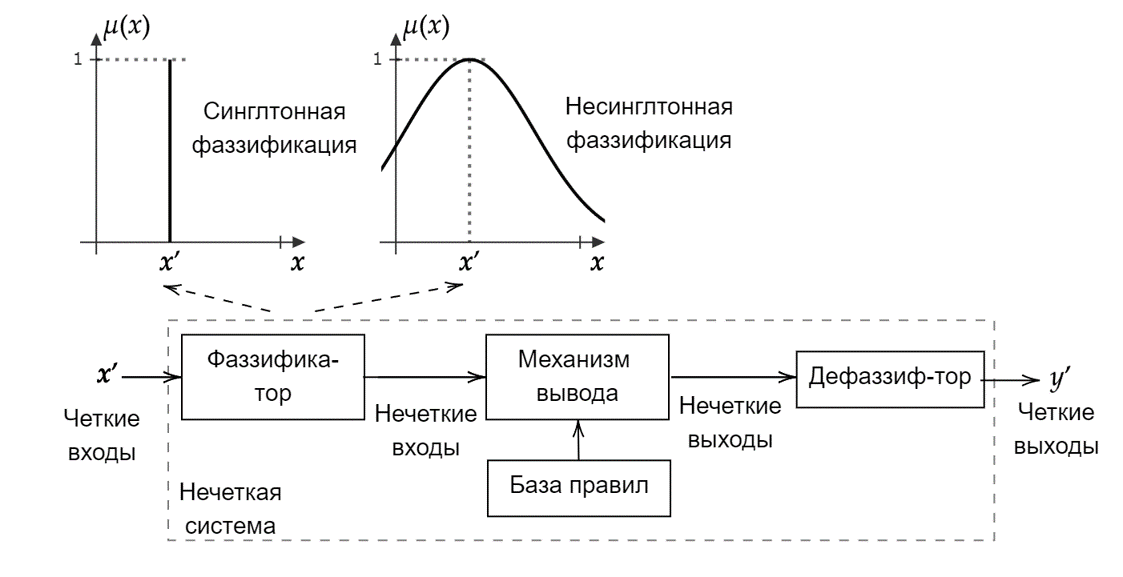
\includegraphics[scale=0.6]{singleton-vs-nonsingleton-fs}}
	\caption{Схема системы нечеткого вывода с использованием синглтонной и несинглтонной фаззификации}
	\label{fig:singleton-vs-nonsingleton}
\end{figure}

Нечеткая система представляется в виде композиции фаззификатора, базы правил, модуля вывода и дефаззификатора, как показано ра рисунке \cref{fig.signleton-vs-nonsingleton}. Фаззификация --- отображение входных данных из исходного пространства в пространство нечетких множеств. Наиболее распространенным является метод синглтонной фаззфикации. Основная причина его широкого использования является существенное упрощение реализации систем нечеткого вывода. При использовании синглтонной фаззификации поданное на вход значение $x'$ интерпретируется как истинное значение измеренной величины, что эквивалентно использованию функции принадлежности входного нечеткого множества $\mu_{A'}(x) = \left[x = x'\right]$. Информация о неопределенности входных данных при этом игнорируется.

Альтернативный подход с использованием несинглтонной фаззификации предусматривает формализацию входного значения нечетким множеством, содержащим информацию о неопределенности значения точки входных данных. Эти неопределенности могут возникать как результат несовершенства процедуры измерений (например, шумом измерительного оборудования, дефектами или деградацией качества датчиков), или когда входные данные описываются качественными понятиями естественного языка.

В случае с анализом числовых данных, неопределенность измерений формализуется функцией принадлежности, которая $\mu_{A'}(x') = 1$ и $\mu_{A'}(x)$ уменьшается по мере удаления от $x'$. При таком способе моделирования измеренное значение $x'$ рассматривается как истинное, а значения в его окрестности --- как возможные.

\begin{figure}[ht]
	\begin{minipage}[b][][b]{0.3\linewidth}
		\centering
		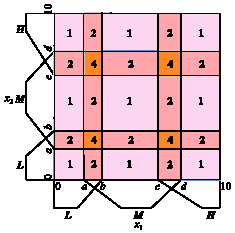
\includegraphics[width=\linewidth, page=1]{ns-fuz-mendel-comparizon-first-order-partition} \\ а) $\sigma_{A'} = 0\%$
	\end{minipage}
	\hfill
	\begin{minipage}[b][][b]{0.3\linewidth}
		\centering
		\includegraphics[width=\linewidth, page=2]{ns-fuz-mendel-comparizon-first-order-partition} \\ б) $\sigma_{A'} = 4\%$
	\end{minipage}
	\hfill
	\begin{minipage}[b][][b]{0.3\linewidth}
		\centering
		\includegraphics[width=\linewidth, page=3]{ns-fuz-mendel-comparizon-first-order-partition} \\ в)  $\sigma_{A'} = 12\%$
	\end{minipage}

    \caption{Сравнение областей активации правил при переходе от синглтонной фаззификации к несинглтонной и при увеличении ширины окрестности погрешности $\sigma_{A'}$.}
\end{figure}

Влияние перехода от синглтонной фаззификации к несинглтонной и величины окрестности погрешности на внутренее поведение и итоговое качество нечеткой системы продемонстрировал Мендель в \cite{Mendel2021, Mendel2017}. 

Для анализа влияния от использования того или иного способа фаззификации на корректность получаемого результата в статье \cite{Mendel2020} рассматривается карта разбиений первого и второго порядка на декартовом произведении базовых множеств входных лингвистических переменных. Мендель в своей книге проводил такое сравнение для систем типа Мамдани. Поскольку в системах типа Мамдани в качестве функции импликации выступает $t$-норма, то разница от применения двух способов фаззификации проявляется в различных максимальных уровнях линии пересечения ф. п. входной посылки и антецедента правила. %В зависимости от минимум или произведение. 

Применение композиционного правила вывода $\sup$ здесь дает эффект \textit{префильтрации} (или \textit{корректировки}) входного значения. То есть ядра функций принадлежности антецедентов правил выполняют функцию эталонов, а уровень пересечения функции принадлежности для входного значения и ф. п. антецедента правила позволяет интерпретировать входное значение как суперпозицию эталонных значений антецедентов с долями равными этому уровню.

 %Разбиение первого порядка 

\pgfmathdeclarefunction{gauss}{3}{%
  \pgfmathparse{exp(-((#1-#2)/(2*#3))^2)} % Correct syntax for Gaussian function
}
\pgfmathdeclarefunction{implL}{4}{%
  \pgfmathparse{min(1, 1-#4+gauss(#1, #2, #3))} % Lukasievich
}
\pgfmathdeclarefunction{implR}{4}{%
  \pgfmathparse{min(1, gauss(#1, #2, #3)/#4)} % R
}

\pgfplotsset{
    membership axes/.style={
        width=0.20\textwidth,
        height=0.20\textwidth,
        scale only axis,
        domain=0:1,
        samples=100,
        every axis plot/.append style={smooth},
        axis lines=middle,
        xmin=0, xmax=1,
        ymin=0, ymax=1,
        xticklabel style={font=\tiny, inner sep=1pt, outer sep=0pt},
        yticklabel style={font=\tiny, inner sep=1pt, outer sep=0pt},
    }
}

\begin{figure}[ht]
    \centering
    \begin{subfigure}[b]{\textwidth}
        \begin{tikzpicture}

        %\begin{scope}[xshift=0cm, yshift=0cm]
            \pgfmathsetmacro{\aZeroMu}{0.55}
            \pgfmathsetmacro{\aFstMu}{0.28}
            \pgfmathsetmacro{\aFstSigma}{0.09}
            \pgfmathsetmacro{\aFstCrossX}{0.55}
            \pgfmathsetmacro{\aFstCrossY}{0.11}
            \pgfmathsetmacro{\aSndMu}{0.5}
            \pgfmathsetmacro{\aSndSigma}{0.08}
            \pgfmathsetmacro{\aSndCrossX}{0.55}
            \pgfmathsetmacro{\aSndCrossY}{0.91}
            \pgfmathsetmacro{\aTrdMu}{0.89}
            \pgfmathsetmacro{\aTrdSigma}{0.2}
            \pgfmathsetmacro{\aTrdCrossX}{0.55}
            \pgfmathsetmacro{\aTrdCrossY}{0.49}
            \pgfmathsetmacro{\bFstMu}{0.2}
            \pgfmathsetmacro{\bFstSigma}{0.12}
            \pgfmathsetmacro{\bSndMu}{0.5}
            \pgfmathsetmacro{\bSndSigma}{0.1}
            \pgfmathsetmacro{\bTrdMu}{0.8}
            \pgfmathsetmacro{\bTrdSigma}{0.1}

            % First function
            \begin{axis}[
                membership axes,
                name=plot1,
                at={(0,0)},
                xlabel={$x_1$},
                ylabel={$\mu$},
                xlabel style={font=\footnotesize, at=(current axis.south), anchor=north, yshift=-10pt},
                ylabel style={font=\footnotesize, at=(current axis.west), anchor=east, xshift=-10pt},
            ]
                \addplot[blue, name path=A0] coordinates {(\aZeroMu, 0) (\aZeroMu, 1)};
                \addplot[black, name path=A1] {gauss(\x, \aFstMu, \aFstSigma)};
                \addplot[only marks, mark=*, mark size=2pt, purple!50] coordinates {(\aFstCrossX,\aFstCrossY)};
                \coordinate (fire11) at (axis cs:\aFstCrossX,\aFstCrossY); % USE axis cs
            \end{axis}
            % Second function
            \begin{axis}[
                membership axes,
                name=plot2,
                at={(0.25\textwidth,0)},
                xlabel={$x_2$},
                ylabel={$\mu$},
                xlabel style={font=\footnotesize, at=(current axis.south), anchor=north, yshift=-10pt},
                ylabel style={font=\footnotesize, at=(current axis.west), anchor=east, xshift=-10pt},
            ]
                \addplot[blue, name path=A0] coordinates {(\aZeroMu, 0) (\aZeroMu, 1)};
                \addplot[black, name path=A1] {gauss(\x, \aSndMu, \aSndSigma)};
                \addplot[only marks, mark=*, mark size=2pt, lime] coordinates {(\aSndCrossX,\aSndCrossY)};
                \coordinate (fire12) at (axis cs:\aSndCrossX,\aSndCrossY); % Use axis cs
            \end{axis}
            % Third function
            \begin{axis}[
                membership axes,
                name=plot3,
                at={(0.5\textwidth,0)},
                xlabel={$x_3$},
                ylabel={$\mu$},
                xlabel style={font=\footnotesize, at=(current axis.south), anchor=north, yshift=-10pt},
                ylabel style={font=\footnotesize, at=(current axis.west), anchor=east, xshift=-10pt},
            ]
                \addplot[blue, name path=A0] coordinates {(\aZeroMu, 0) (\aZeroMu, 1)};
                \addplot[black, name path=A1] {gauss(\x, \aTrdMu, \aTrdSigma)};
                \addplot[only marks, mark=*, mark size=2pt, cyan!50] coordinates {(\aTrdCrossX,\aTrdCrossY)};
                \coordinate (fire13) at (axis cs:\aTrdCrossX,\aTrdCrossY); % Use axis cs
            \end{axis}
            % Fourth function
            \begin{axis}[
                membership axes,
                name=plot4,
                at={(0.75\textwidth,0)},
                xlabel={$y$},
                ylabel={$\mu_{B'}(y)$},
                xlabel style={font=\footnotesize, at=(current axis.south), anchor=north, yshift=-10pt},
                ylabel style={font=\footnotesize, at=(current axis.above origin), anchor=south},
            ]
                \addplot [purple!50] {min(\aFstCrossY, gauss(\x, \bFstMu, \bFstSigma))};
                \addplot [lime] {min(\aSndCrossY, gauss(\x, \bSndMu, \bSndSigma))};
                \addplot [cyan!50] {min(\aTrdCrossY, gauss(\x, \bTrdMu, \bTrdSigma))};
                \addplot[fill=orange!30, orange] {max(min(\aFstCrossY, gauss(\x, \bFstMu, \bFstSigma)), min(\aSndCrossY, gauss(\x, \bSndMu, \bSndSigma)), min(\aTrdCrossY, gauss(\x, \bTrdMu, \bTrdSigma)))} \closedcycle;
                \coordinate (out11) at (axis cs:0.0,\aFstCrossY); % Use axis cs
                \coordinate (out12) at (axis cs:0.0,\aSndCrossY); % Use axis cs
                \coordinate (out13) at (axis cs:0.0,\aTrdCrossY); % Use axis cs
            \end{axis}

            % Connect coordinates using defined coordinate names
            \draw [purple!50, dashed, thick] (fire11) -- (out11);
            \draw [lime, dashed, thick] (fire12) -- (out12);
            \draw [cyan!50, dashed, thick] (fire13) -- (out13);

            % \node {\sigma=\aZeroSigma};
            \node[left, xshift=-1.2cm, font=\footnotesize, rotate=90, anchor=center] at (plot1.west) {$\sigma_{A'}=0$};
        \end{tikzpicture}
	\end{subfigure}
	
	%%
	\vspace{0.1cm}
	%%
	
	\begin{subfigure}[b]{\textwidth}
        \begin{tikzpicture}

        %\begin{scope}[xshift=0cm, yshift=0cm]
            \pgfmathsetmacro{\aZeroMu}{0.55}
            \pgfmathsetmacro{\aZeroSigma}{0.01}
            \pgfmathsetmacro{\aFstMu}{0.28}
            \pgfmathsetmacro{\aFstSigma}{0.09}
            \pgfmathsetmacro{\aFstCrossX}{0.515}
            \pgfmathsetmacro{\aFstCrossY}{0.185}
            \pgfmathsetmacro{\aSndMu}{0.5}
            \pgfmathsetmacro{\aSndSigma}{0.08}
            \pgfmathsetmacro{\aSndCrossX}{0.56}
            \pgfmathsetmacro{\aSndCrossY}{0.88}
            \pgfmathsetmacro{\aTrdMu}{0.89}
            \pgfmathsetmacro{\aTrdSigma}{0.2}
            \pgfmathsetmacro{\aTrdCrossX}{0.57}
            \pgfmathsetmacro{\aTrdCrossY}{0.53}
            \pgfmathsetmacro{\bFstMu}{0.2}
            \pgfmathsetmacro{\bFstSigma}{0.12}
            \pgfmathsetmacro{\bSndMu}{0.5}
            \pgfmathsetmacro{\bSndSigma}{0.1}
            \pgfmathsetmacro{\bTrdMu}{0.8}
            \pgfmathsetmacro{\bTrdSigma}{0.1}

            % First function
            \begin{axis}[
                membership axes,
                name=plot1,
                at={(0,0)},
                xlabel={$x_1$},
                ylabel={$\mu$},
                xlabel style={},
                xlabel style={font=\footnotesize, at=(current axis.south), anchor=north, yshift=-10pt},
                ylabel style={font=\footnotesize, at=(current axis.west), anchor=east, xshift=-10pt},
            ]
                \addplot[blue, name path=A0] {gauss(\x, \aZeroMu, \aZeroSigma)};
                \addplot[black, name path=A1] {gauss(\x, \aFstMu, \aFstSigma)};
                \addplot[fill=purple!50, draw=none] {min(gauss(\x, \aZeroMu, \aZeroSigma), gauss(\x, \aFstMu, \aFstSigma))} \closedcycle;
                \coordinate (fire11) at (axis cs:\aFstCrossX,\aFstCrossY); % USE axis cs
            \end{axis}
            % Second function
            \begin{axis}[
                membership axes,
                name=plot2,
                at={(0.25\textwidth,0)},
                xlabel={$x_2$},
                ylabel={$\mu$},
                xlabel style={font=\footnotesize, at=(current axis.south), anchor=north, yshift=-10pt},
                ylabel style={font=\footnotesize, at=(current axis.west), anchor=east, xshift=-10pt},
            ]
                \addplot[blue, name path=A0] {gauss(\x, \aZeroMu, \aZeroSigma)};
                \addplot[black, name path=A1] {gauss(\x, \aSndMu, \aSndSigma)};
                \addplot[fill=lime, draw=none] {min(gauss(\x, \aZeroMu, \aZeroSigma), gauss(\x, \aSndMu, \aSndSigma))} \closedcycle;
                \coordinate (fire12) at (axis cs:\aSndCrossX,\aSndCrossY); % Use axis cs
            \end{axis}
            % Third function
            \begin{axis}[
                membership axes,
                name=plot3,
                at={(0.5\textwidth,0)},
                xlabel={$x_3$},
                ylabel={$\mu$},
                xlabel style={font=\footnotesize, at=(current axis.south), anchor=north, yshift=-10pt},
                ylabel style={font=\footnotesize, at=(current axis.west), anchor=east, xshift=-10pt},
            ]
                \addplot[blue, name path=A0] {gauss(\x, \aZeroMu, \aZeroSigma)};
                \addplot[black, name path=A1] {gauss(\x, \aTrdMu, \aTrdSigma)};
                \addplot[fill=cyan!50, draw=none] {min(gauss(\x, \aZeroMu, \aZeroSigma), gauss(\x, \aTrdMu, \aTrdSigma))} \closedcycle;
                \coordinate (fire13) at (axis cs:\aTrdCrossX,\aTrdCrossY); % Use axis cs
            \end{axis}
            % Fourth function
            \begin{axis}[
                membership axes,
                name=plot4,
                at={(0.75\textwidth,0)},
                xlabel={$y$},
                ylabel={$\mu_{B'}(y)$},
                xlabel style={font=\footnotesize, at=(current axis.south), anchor=north, yshift=-10pt},
                ylabel style={font=\footnotesize, at=(current axis.above origin), anchor=south},
            ]
                \addplot [purple!50] {min(\aFstCrossY, gauss(\x, \bFstMu, \bFstSigma))};
                \addplot [lime] {min(\aSndCrossY, gauss(\x, \bSndMu, \bSndSigma))};
                \addplot [cyan!50] {min(\aTrdCrossY, gauss(\x, \bTrdMu, \bTrdSigma))};
                \addplot[fill=orange!30, orange] {max(min(\aFstCrossY, gauss(\x, \bFstMu, \bFstSigma)), min(\aSndCrossY, gauss(\x, \bSndMu, \bSndSigma)), min(\aTrdCrossY, gauss(\x, \bTrdMu, \bTrdSigma)))} \closedcycle;
                \coordinate (out11) at (axis cs:0.0,\aFstCrossY); % Use axis cs
                \coordinate (out12) at (axis cs:0.0,\aSndCrossY); % Use axis cs
                \coordinate (out13) at (axis cs:0.0,\aTrdCrossY); % Use axis cs
            \end{axis}

            % Connect coordinates using defined coordinate names
            \draw [purple!50, dashed, thick] (fire11) -- (out11);
            \draw [lime, dashed, thick] (fire12) -- (out12);
            \draw [cyan!50, dashed, thick] (fire13) -- (out13);

            % \node {\sigma=\aZeroSigma};
            \node[left, xshift=-1.2cm, font=\footnotesize, rotate=90, anchor=center] at (plot1.west) {$\sigma_{A'}=\aZeroSigma$};
        \end{tikzpicture}
	\end{subfigure}
	
	%%
	\vspace{0.1cm}
	%%
	
	\begin{subfigure}[b]{\textwidth}
          \begin{tikzpicture}
            \pgfmathsetmacro{\aZeroMu}{0.55}
            \pgfmathsetmacro{\aZeroSigma}{0.05}
            \pgfmathsetmacro{\aFstMu}{0.28}
            \pgfmathsetmacro{\aFstSigma}{0.09}
            \pgfmathsetmacro{\aFstCrossX}{0.49}
            \pgfmathsetmacro{\aFstCrossY}{0.4}
            \pgfmathsetmacro{\aSndMu}{0.5}
            \pgfmathsetmacro{\aSndSigma}{0.08}
            \pgfmathsetmacro{\aSndCrossX}{0.53}
            \pgfmathsetmacro{\aSndCrossY}{0.97}
            \pgfmathsetmacro{\aTrdMu}{0.89}
            \pgfmathsetmacro{\aTrdSigma}{0.2}
            \pgfmathsetmacro{\aTrdCrossX}{0.6}
            \pgfmathsetmacro{\aTrdCrossY}{0.61}
            \pgfmathsetmacro{\bFstMu}{0.2}
            \pgfmathsetmacro{\bFstSigma}{0.12}
            \pgfmathsetmacro{\bSndMu}{0.5}
            \pgfmathsetmacro{\bSndSigma}{0.1}
            \pgfmathsetmacro{\bTrdMu}{0.8}
            \pgfmathsetmacro{\bTrdSigma}{0.1}

            % First function
            \begin{axis}[
                membership axes,
                name=plot1,
                at={(0,0)},
                xlabel={$x_1$},
                ylabel={$\mu$},
                xlabel style={font=\footnotesize, at=(current axis.south), anchor=north, yshift=-10pt},
                ylabel style={font=\footnotesize, at=(current axis.west), anchor=east, xshift=-10pt},
            ]
                \addplot[blue, name path=A0] {gauss(\x, \aZeroMu, \aZeroSigma)};
                \addplot[black, name path=A1] {gauss(\x, \aFstMu, \aFstSigma)};
                \addplot[fill=purple!50, draw=none] {min(gauss(\x, \aZeroMu, \aZeroSigma), gauss(\x, \aFstMu, \aFstSigma))} \closedcycle;
                \coordinate (fire11) at (axis cs:\aFstCrossX,\aFstCrossY); % USE axis cs
            \end{axis}
            % Second function
            \begin{axis}[
                membership axes,
                name=plot2,
                at={(0.25\textwidth,0)},
                xlabel={$x_2$},
                ylabel={$\mu$},
                xlabel style={font=\footnotesize, at=(current axis.south), anchor=north, yshift=-10pt},
                ylabel style={font=\footnotesize, at=(current axis.west), anchor=east, xshift=-10pt},
            ]
                \addplot[blue, name path=A0] {gauss(\x, \aZeroMu, \aZeroSigma)};
                \addplot[black, name path=A1] {gauss(\x, \aSndMu, \aSndSigma)};
                \addplot[fill=lime, draw=none] {min(gauss(\x, \aZeroMu, \aZeroSigma), gauss(\x, \aSndMu, \aSndSigma))} \closedcycle;
                \coordinate (fire12) at (axis cs:\aSndCrossX,\aSndCrossY); % Use axis cs
            \end{axis}
            % Third function
            \begin{axis}[
                membership axes,
                name=plot2,
                at={(0.5\textwidth,0)},
                xlabel={$x_3$},
                ylabel={$\mu$},
                xlabel style={font=\footnotesize, at=(current axis.south), anchor=north, yshift=-10pt},
                ylabel style={font=\footnotesize, at=(current axis.west), anchor=east, xshift=-10pt},
            ]
                \addplot[blue, name path=A0] {gauss(\x, \aZeroMu, \aZeroSigma)};
                \addplot[black, name path=A1] {gauss(\x, \aTrdMu, \aTrdSigma)};
                \addplot[fill=cyan!50, draw=none] {min(gauss(\x, \aZeroMu, \aZeroSigma), gauss(\x, \aTrdMu, \aTrdSigma))} \closedcycle;
                \coordinate (fire13) at (axis cs:\aTrdCrossX,\aTrdCrossY); % Use axis cs
            \end{axis}
            % Fourth function
            \begin{axis}[
                membership axes,
                name=plot4,
                at={(0.75\textwidth,0)},
                xlabel={$y$},
                ylabel={$\mu_{B'}(y)$},
                xlabel style={font=\footnotesize, at=(current axis.south), anchor=north, yshift=-10pt},
                ylabel style={font=\footnotesize, at=(current axis.above origin), anchor=south},
            ]
                \addplot [purple!50] {min(\aFstCrossY, gauss(\x, \bFstMu, \bFstSigma))};
                \addplot [lime] {min(\aSndCrossY, gauss(\x, \bSndMu, \bSndSigma))};
                \addplot [cyan!50] {min(\aTrdCrossY, gauss(\x, \bTrdMu, \bTrdSigma))};
                \addplot[fill=orange!30, orange] {max(min(\aFstCrossY, gauss(\x, \bFstMu, \bFstSigma)), min(\aSndCrossY, gauss(\x, \bSndMu, \bSndSigma)), min(\aTrdCrossY, gauss(\x, \bTrdMu, \bTrdSigma)))} \closedcycle;
                \coordinate (out11) at (axis cs:0.0,\aFstCrossY); % Use axis cs
                \coordinate (out12) at (axis cs:0.0,\aSndCrossY); % Use axis cs
                \coordinate (out13) at (axis cs:0.0,\aTrdCrossY); % Use axis cs
            \end{axis}

            % Connect coordinates using defined coordinate names
            \draw [purple!50, dashed, thick] (fire11) -- (out11);
            \draw [lime, dashed, thick] (fire12) -- (out12);
            \draw [cyan!50, dashed, thick] (fire13) -- (out13);

            % \node {\sigma=\aZeroSigma};
            \node[left, xshift=-1.2cm, font=\footnotesize, rotate=90, anchor=center] at (plot1.west) {$\sigma_{A'}=\aZeroSigma$};
        \end{tikzpicture}
    \end{subfigure}
    \caption{Сравнение формы функций принадлежности выходных нечетких множеств для подхода Мамдани}
    \label{fig:ns-width-influence-to-out-mamdani}
\end{figure}

Показанная на этих схемах динамика более ясно раскрыта на рисунке \cref{fig:ns-width-influence-to-out-mamdani} для различных значениях среднеквадратичного отклонения в гауссовой ф. п. входного значения на примере агрегации выходной ф. п. нечеткой системы с тремя правилами в базе правил. Видно, что при переходе от синглтонной фаззификации к несинглтонной и при дальнейшем увеличении ширины среднеквадратичного отклонения ф. п. входного нечеткого множества, повышается уровень срабатывания первого правила, и, как следствие использования импликации Мамдани, уровень задействования ф. п. выходного нечеткого множества этого правила в результирующей агрегации. Кроме того, можно пронаблюдать, упомянутый ранее, эффект корректировки входного значения антецедентом третьего правила.

В случае с нечеткой системой логического типа, разница от использования различных способов фаззификации будет проявляться в различных формах выходного нечеткого множества. 

\begin{figure}[ht]
    \centering
    \begin{subfigure}[b]{\textwidth}
        \begin{tikzpicture}

        %\begin{scope}[xshift=0cm, yshift=0cm]
            \pgfmathsetmacro{\aZeroMu}{0.55}
            \pgfmathsetmacro{\aFstMu}{0.28}
            \pgfmathsetmacro{\aFstSigma}{0.09}
            \pgfmathsetmacro{\aFstCrossX}{0.55}
            \pgfmathsetmacro{\aFstCrossY}{0.11}
            \pgfmathsetmacro{\aSndMu}{0.5}
            \pgfmathsetmacro{\aSndSigma}{0.08}
            \pgfmathsetmacro{\aSndCrossX}{0.55}
            \pgfmathsetmacro{\aSndCrossY}{0.91}
            \pgfmathsetmacro{\aTrdMu}{0.89}
            \pgfmathsetmacro{\aTrdSigma}{0.2}
            \pgfmathsetmacro{\aTrdCrossX}{0.55}
            \pgfmathsetmacro{\aTrdCrossY}{0.49}
            \pgfmathsetmacro{\bFstMu}{0.2}
            \pgfmathsetmacro{\bFstSigma}{0.12}
            \pgfmathsetmacro{\bSndMu}{0.5}
            \pgfmathsetmacro{\bSndSigma}{0.1}
            \pgfmathsetmacro{\bTrdMu}{0.8}
            \pgfmathsetmacro{\bTrdSigma}{0.1}

            % First function
            \begin{axis}[
                membership axes,
                name=plot1,
                at={(0,0)},
                xlabel={$x_1$},
                ylabel={$\mu$},
                xlabel style={font=\footnotesize, at=(current axis.south), anchor=north},
                ylabel style={font=\footnotesize, at=(current axis.west), anchor=east, xshift=-10pt},
                y dir=reverse,
                % axis x line=top,
                xticklabel pos=upper,
                xticklabel style={yshift=13pt}
            ]
                \addplot[blue, name path=A0] coordinates {(\aZeroMu, 0) (\aZeroMu, 1)};
                \addplot[black, name path=A1] {gauss(\x, \aFstMu, \aFstSigma)};
                \addplot[only marks, mark=*, mark size=2pt, purple!50] coordinates {(\aFstCrossX,\aFstCrossY)};
                \coordinate (fire11) at (axis cs:\aFstCrossX,\aFstCrossY); % USE axis cs
            \end{axis}
            % Second function
            \begin{axis}[
                membership axes,
                name=plot2,
                at={(0.25\textwidth,0)},
                xlabel={$x_2$},
                ylabel={$\mu$},
                xlabel style={font=\footnotesize, at=(current axis.south), anchor=north},
                ylabel style={font=\footnotesize, at=(current axis.west), anchor=east, xshift=-10pt},
                y dir=reverse,
                % axis x line=top,
                xticklabel pos=upper,
                xticklabel style={yshift=13pt}
            ]
                \addplot[blue, name path=A0] coordinates {(\aZeroMu, 0) (\aZeroMu, 1)};
                \addplot[black, name path=A1] {gauss(\x, \aSndMu, \aSndSigma)};
                \addplot[only marks, mark=*, mark size=2pt, lime] coordinates {(\aSndCrossX,\aSndCrossY)};
                \coordinate (fire12) at (axis cs:\aSndCrossX,\aSndCrossY); % Use axis cs
            \end{axis}
            % Third function
            \begin{axis}[
                membership axes,
                name=plot3,
                at={(0.5\textwidth,0)},
                xlabel={$x_3$},
                ylabel={$\mu$},
                xlabel style={font=\footnotesize, at=(current axis.south), anchor=north},
                ylabel style={font=\footnotesize, at=(current axis.west), anchor=east, xshift=-10pt},
                y dir=reverse,
                % axis x line=top,
                xticklabel pos=upper,
                xticklabel style={yshift=13pt}
            ]
                \addplot[blue, name path=A0] coordinates {(\aZeroMu, 0) (\aZeroMu, 1)};
                \addplot[black, name path=A1] {gauss(\x, \aTrdMu, \aTrdSigma)};
                \addplot[only marks, mark=*, mark size=2pt, cyan!50] coordinates {(\aTrdCrossX,\aTrdCrossY)};
                \coordinate (fire13) at (axis cs:\aTrdCrossX,\aTrdCrossY); % Use axis cs
            \end{axis}
            % Fourth function
            \begin{axis}[
                membership axes,
                name=plot4,
                at={(0.75\textwidth,0)},
                xlabel={$y$},
                ylabel={$\mu_{B'}(y)$},
                xlabel style={font=\footnotesize, at=(current axis.south), anchor=north, yshift=-10pt},
                ylabel style={font=\footnotesize, at=(current axis.above origin), anchor=south},
            ]
                \addplot [purple!50] {implL(\x, \bFstMu, \bFstSigma, \aFstCrossY)};
                \addplot [lime] {implL(\x, \bSndMu, \bSndSigma, \aSndCrossY)};
                \addplot [cyan!50] {implL(\x, \bTrdMu, \bTrdSigma, \aTrdCrossY)};
                \addplot[fill=orange!30, orange] {min(implL(\x, \bFstMu, \bFstSigma, \aFstCrossY), implL(\x, \bSndMu, \bSndSigma, \aSndCrossY), implL(\x, \bTrdMu, \bTrdSigma, \aTrdCrossY))} \closedcycle;
                \coordinate (out11) at (axis cs:0.0,1-\aFstCrossY); % Use axis cs
                \coordinate (out12) at (axis cs:0.0,1-\aSndCrossY); % Use axis cs
                \coordinate (out13) at (axis cs:0.0,1-\aTrdCrossY); % Use axis cs
            \end{axis}

            % Connect coordinates using defined coordinate names
            \draw [purple!50, dashed, thick] (fire11) -- (out11);
            \draw [lime, dashed, thick] (fire12) -- (out12);
            \draw [cyan!50, dashed, thick] (fire13) -- (out13);

            % \node {\sigma=\aZeroSigma};
            \node[left, xshift=-1.2cm, font=\footnotesize, rotate=90, anchor=center] at (plot1.west) {$\sigma_{A'}=0$};
        \end{tikzpicture}
	\end{subfigure}
	
	%%
	\vspace{0.1cm}
	%%
	
	\begin{subfigure}[b]{\textwidth}
        \begin{tikzpicture}

        %\begin{scope}[xshift=0cm, yshift=0cm]
            \pgfmathsetmacro{\aZeroMu}{0.55}
            \pgfmathsetmacro{\aZeroSigma}{0.01}
            \pgfmathsetmacro{\aFstMu}{0.28}
            \pgfmathsetmacro{\aFstSigma}{0.09}
            \pgfmathsetmacro{\aFstCrossX}{0.515}
            \pgfmathsetmacro{\aFstCrossY}{0.185}
            \pgfmathsetmacro{\aSndMu}{0.5}
            \pgfmathsetmacro{\aSndSigma}{0.08}
            \pgfmathsetmacro{\aSndCrossX}{0.56}
            \pgfmathsetmacro{\aSndCrossY}{0.88}
            \pgfmathsetmacro{\aTrdMu}{0.89}
            \pgfmathsetmacro{\aTrdSigma}{0.2}
            \pgfmathsetmacro{\aTrdCrossX}{0.57}
            \pgfmathsetmacro{\aTrdCrossY}{0.53}
            \pgfmathsetmacro{\bFstMu}{0.2}
            \pgfmathsetmacro{\bFstSigma}{0.12}
            \pgfmathsetmacro{\bSndMu}{0.5}
            \pgfmathsetmacro{\bSndSigma}{0.1}
            \pgfmathsetmacro{\bTrdMu}{0.8}
            \pgfmathsetmacro{\bTrdSigma}{0.1}

            % First function
            \begin{axis}[
                membership axes,
                name=plot1,
                at={(0,0)},
                xlabel={$x_1$},
                ylabel={$\mu$},
                xlabel style={font=\footnotesize, at=(current axis.south), anchor=north},
                ylabel style={font=\footnotesize, at=(current axis.west), anchor=east, xshift=-10pt},
                y dir=reverse,
                % axis x line=top,
                xticklabel pos=upper,
                xticklabel style={yshift=13pt}
            ]
                \addplot[blue, name path=A0] {gauss(\x, \aZeroMu, \aZeroSigma)};
                \addplot[black, name path=A1] {gauss(\x, \aFstMu, \aFstSigma)};
                \addplot[fill=purple!50, draw=none] {min(gauss(\x, \aZeroMu, \aZeroSigma), gauss(\x, \aFstMu, \aFstSigma))} \closedcycle;
                \coordinate (fire11) at (axis cs:\aFstCrossX,\aFstCrossY); % USE axis cs
            \end{axis}
            % Second function
            \begin{axis}[
                membership axes,
                name=plot2,
                at={(0.25\textwidth,0)},
                xlabel={$x_2$},
                ylabel={$\mu$},
                xlabel style={font=\footnotesize, at=(current axis.south), anchor=north},
                ylabel style={font=\footnotesize, at=(current axis.west), anchor=east, xshift=-10pt},
                y dir=reverse,
                % axis x line=top,
                xticklabel pos=upper,
                xticklabel style={yshift=13pt}
            ]
                \addplot[blue, name path=A0] {gauss(\x, \aZeroMu, \aZeroSigma)};
                \addplot[black, name path=A1] {gauss(\x, \aSndMu, \aSndSigma)};
                \addplot[fill=lime, draw=none] {min(gauss(\x, \aZeroMu, \aZeroSigma), gauss(\x, \aSndMu, \aSndSigma))} \closedcycle;
                \coordinate (fire12) at (axis cs:\aSndCrossX,\aSndCrossY); % Use axis cs
            \end{axis}
            % Third function
            \begin{axis}[
                membership axes,
                name=plot3,
                at={(0.5\textwidth,0)},
                xlabel={$x_3$},
                ylabel={$\mu$},
                xlabel style={font=\footnotesize, at=(current axis.south), anchor=north},
                ylabel style={font=\footnotesize, at=(current axis.west), anchor=east, xshift=-10pt},
                y dir=reverse,
                % axis x line=top,
                xticklabel pos=upper,
                xticklabel style={yshift=13pt}
            ]
                \addplot[blue, name path=A0] {gauss(\x, \aZeroMu, \aZeroSigma)};
                \addplot[black, name path=A1] {gauss(\x, \aTrdMu, \aTrdSigma)};
                \addplot[fill=cyan!50, draw=none] {min(gauss(\x, \aZeroMu, \aZeroSigma), gauss(\x, \aTrdMu, \aTrdSigma))} \closedcycle;
                \coordinate (fire13) at (axis cs:\aTrdCrossX,\aTrdCrossY); % Use axis cs
            \end{axis}
            % Fourth function
            \begin{axis}[
                membership axes,
                name=plot4,
                at={(0.75\textwidth,0)},
                xlabel={$y$},
                ylabel={$\mu_{B'}(y)$},
                xlabel style={font=\footnotesize, at=(current axis.south), anchor=north, yshift=-10pt},
                ylabel style={font=\footnotesize, at=(current axis.above origin), anchor=south},
            ]
                \addplot [purple!50] {implL(\x, \bFstMu, \bFstSigma, \aFstCrossY)};
                \addplot [lime] {implL(\x, \bSndMu, \bSndSigma, \aSndCrossY)};
                \addplot [cyan!50] {implL(\x, \bTrdMu, \bTrdSigma, \aTrdCrossY)};
                \addplot[fill=orange!30, orange] {min(implL(\x, \bFstMu, \bFstSigma, \aFstCrossY), implL(\x, \bSndMu, \bSndSigma, \aSndCrossY), implL(\x, \bTrdMu, \bTrdSigma, \aTrdCrossY))} \closedcycle;
                \coordinate (out11) at (axis cs:0.0,1-\aFstCrossY); % Use axis cs
                \coordinate (out12) at (axis cs:0.0,1-\aSndCrossY); % Use axis cs
                \coordinate (out13) at (axis cs:0.0,1-\aTrdCrossY); % Use axis cs
            \end{axis}

            % Connect coordinates using defined coordinate names
            \draw [purple!50, dashed, thick] (fire11) -- (out11);
            \draw [lime, dashed, thick] (fire12) -- (out12);
            \draw [cyan!50, dashed, thick] (fire13) -- (out13);

            % \node {\sigma=\aZeroSigma};
            \node[left, xshift=-1.2cm, font=\footnotesize, rotate=90, anchor=center] at (plot1.west) {$\sigma_{A'}=\aZeroSigma$};
        \end{tikzpicture}
	\end{subfigure}
	
	%%
	\vspace{0.1cm}
	%%
	
	\begin{subfigure}[b]{\textwidth}
          \begin{tikzpicture}
            \pgfmathsetmacro{\aZeroMu}{0.55}
            \pgfmathsetmacro{\aZeroSigma}{0.05}
            \pgfmathsetmacro{\aFstMu}{0.28}
            \pgfmathsetmacro{\aFstSigma}{0.09}
            \pgfmathsetmacro{\aFstCrossX}{0.49}
            \pgfmathsetmacro{\aFstCrossY}{0.4}
            \pgfmathsetmacro{\aSndMu}{0.5}
            \pgfmathsetmacro{\aSndSigma}{0.08}
            \pgfmathsetmacro{\aSndCrossX}{0.53}
            \pgfmathsetmacro{\aSndCrossY}{0.97}
            \pgfmathsetmacro{\aTrdMu}{0.89}
            \pgfmathsetmacro{\aTrdSigma}{0.2}
            \pgfmathsetmacro{\aTrdCrossX}{0.6}
            \pgfmathsetmacro{\aTrdCrossY}{0.61}
            \pgfmathsetmacro{\bFstMu}{0.2}
            \pgfmathsetmacro{\bFstSigma}{0.12}
            \pgfmathsetmacro{\bSndMu}{0.5}
            \pgfmathsetmacro{\bSndSigma}{0.1}
            \pgfmathsetmacro{\bTrdMu}{0.8}
            \pgfmathsetmacro{\bTrdSigma}{0.1}

            % First function
            \begin{axis}[
                membership axes,
                name=plot1,
                at={(0,0)},
                xlabel={$x_1$},
                ylabel={$\mu$},
                xlabel style={font=\footnotesize, at=(current axis.south), anchor=north},
                ylabel style={font=\footnotesize, at=(current axis.west), anchor=east, xshift=-10pt},
                y dir=reverse,
                % axis x line=top,
                xticklabel pos=upper,
                xticklabel style={yshift=13pt}
            ]
                \addplot[blue, name path=A0] {gauss(\x, \aZeroMu, \aZeroSigma)};
                \addplot[black, name path=A1] {gauss(\x, \aFstMu, \aFstSigma)};
                \addplot[fill=purple!50, draw=none] {min(gauss(\x, \aZeroMu, \aZeroSigma), gauss(\x, \aFstMu, \aFstSigma))} \closedcycle;
                \coordinate (fire11) at (axis cs:\aFstCrossX,\aFstCrossY); % USE axis cs
            \end{axis}
            % Second function
            \begin{axis}[
                membership axes,
                name=plot2,
                at={(0.25\textwidth,0)},
                xlabel={$x_2$},
                ylabel={$\mu$},
                xlabel style={font=\footnotesize, at=(current axis.south), anchor=north},
                ylabel style={font=\footnotesize, at=(current axis.west), anchor=east, xshift=-10pt},
                y dir=reverse,
                % axis x line=top,
                xticklabel pos=upper,
                xticklabel style={yshift=13pt}
            ]
                \addplot[blue, name path=A0] {gauss(\x, \aZeroMu, \aZeroSigma)};
                \addplot[black, name path=A1] {gauss(\x, \aSndMu, \aSndSigma)};
                \addplot[fill=lime, draw=none] {min(gauss(\x, \aZeroMu, \aZeroSigma), gauss(\x, \aSndMu, \aSndSigma))} \closedcycle;
                \coordinate (fire12) at (axis cs:\aSndCrossX,\aSndCrossY); % Use axis cs
            \end{axis}
            % Third function
            \begin{axis}[
                membership axes,
                name=plot2,
                at={(0.5\textwidth,0)},
                xlabel={$x_3$},
                ylabel={$\mu$},
                xlabel style={font=\footnotesize, at=(current axis.south), anchor=north},
                ylabel style={font=\footnotesize, at=(current axis.west), anchor=east, xshift=-10pt},
                y dir=reverse,
                % axis x line=top,
                xticklabel pos=upper,
                xticklabel style={yshift=13pt}
            ]
                \addplot[blue, name path=A0] {gauss(\x, \aZeroMu, \aZeroSigma)};
                \addplot[black, name path=A1] {gauss(\x, \aTrdMu, \aTrdSigma)};
                \addplot[fill=cyan!50, draw=none] {min(gauss(\x, \aZeroMu, \aZeroSigma), gauss(\x, \aTrdMu, \aTrdSigma))} \closedcycle;
                \coordinate (fire13) at (axis cs:\aTrdCrossX,\aTrdCrossY); % Use axis cs
            \end{axis}
            % Fourth function
            \begin{axis}[
                membership axes,
                name=plot4,
                at={(0.75\textwidth,0)},
                xlabel={$y$},
                ylabel={$\mu_{B'}(y)$},
                xlabel style={font=\footnotesize, at=(current axis.south), anchor=north, yshift=-10pt},
                ylabel style={font=\footnotesize, at=(current axis.above origin), anchor=south},
            ]
                \addplot [purple!50] {implL(\x, \bFstMu, \bFstSigma, \aFstCrossY)};
                \addplot [lime] {implL(\x, \bSndMu, \bSndSigma, \aSndCrossY)};
                \addplot [cyan!50] {implL(\x, \bTrdMu, \bTrdSigma, \aTrdCrossY)};
                \addplot[fill=orange!30, orange] {min(implL(\x, \bFstMu, \bFstSigma, \aFstCrossY), implL(\x, \bSndMu, \bSndSigma, \aSndCrossY), implL(\x, \bTrdMu, \bTrdSigma, \aTrdCrossY))} \closedcycle;
                \coordinate (out11) at (axis cs:0.0,1-\aFstCrossY); % Use axis cs
                \coordinate (out12) at (axis cs:0.0,1-\aSndCrossY); % Use axis cs
                \coordinate (out13) at (axis cs:0.0,1-\aTrdCrossY); % Use axis cs
            \end{axis}

            % Connect coordinates using defined coordinate names
            \draw [purple!50, dashed, thick] (fire11) -- (out11);
            \draw [lime, dashed, thick] (fire12) -- (out12);
            \draw [cyan!50, dashed, thick] (fire13) -- (out13);

            % \node {\sigma=\aZeroSigma};
            \node[left, xshift=-1.2cm, font=\footnotesize, rotate=90, anchor=center] at (plot1.west) {$\sigma_{A'}=\aZeroSigma$};
        \end{tikzpicture}
    \end{subfigure}
    \caption{Сравнение формы функций принадлежности выходных нечетких множеств для логического подхода}
    \label{fig:ns-width-influence-to-out-logical}
\end{figure}


Можно проследить за влиянием увеличения ширины окна для измеренного значения на область выходного нечеткого множества нечеткой системы при использовании логического подхода к нечеткому выводу. При логическом подходе функция принадлежности выходного нечеткого множества формируется как результат пересечения (в данном случае операцией \textit{min}), что можно представить как постепенное вырезание области функции принадлежности выходного нечеткого множества. Из рисунка \cref{fig:ns-width-influence-to-out-logical} видно, что при увеличение ширины в пересечении проекций импликации на пространство выходной переменной оказывается более <<сложно выкроенная>> область.


\section{Нечеткое значение истинности}

\textbf{Определение.} Нечеткой истинностью множества $A$ относительно нечеткого множества $A'$ называется нечеткое множество $CP(A,A')$ такое, что:

\begin{equation}
\label{eqn:1-ftv}
\mu_{CP(A, A')}(v) = \sup_{\substack{\mu_{A}(x) = v \\ x \in X}}\left\{\mu_{A'}(x)\right\}
\end{equation}

\begin{figure}[ht]
	\centering
	\begin{tikzpicture}[
			scale=5,
			%width=15cm, height=15cm,
	]
        % Draw axes
        \draw[->] (0, 0) -- (0, 1) node[above] {$\mu_{CP(A, A')}(v)$};
        \draw[->] (0, 0) -- (1, 0) node[right] {$v = \mu_{A}(x)$};
        \draw[->] (0, 0) -- (0,-1) node[below] {$x$};
        \draw[->] (0, 0) -- (-1, 0) node[left] {$\mu_{A'}(x)$};

	\draw[dashed] (0.3, 0.01) -- (0.3, -0.18054861091112354) -| (-0.0779857041069743, -0.18054861091112354);
	\draw[dashed] (0.3, 0.01) -- (0.3, -0.6194513890888765) -| (-0.6999713601259281, -0.6194513890888765) -| (-0.6999713601259281, 0.6999713601259281) -| (0.3, 0.6999713601259281);

	\node [lime] at (-0.0779857041069743, -0.18054861091112354) {$\mathbf{\times}$};
	\node [red] at (-0.6999713601259281, -0.6194513890888765) {$\mathbf{\times}$};
	\node [red] at (0.3, 0.6999713601259281) {$\mathbf{\times}$};
		
        % Draw Gaussian function
        %\draw[blue, thick, domain=0.01:1, samples=100, smooth] plot (\x, {exp(-((((0.4-0.5) - 0.2*sqrt(-ln(\x)))/0.2)^2)});
        \draw[blue, thick, domain=0.01:1, samples=100, smooth] plot (\x, {exp(-((((0.4-0.5) + 0.2*sqrt(-ln(\x)))/0.2)^2)});
        \draw[blue, thick, domain=0:1, samples=100, smooth] plot ({exp(-((\x-0.4)/0.2)^2)}, -\x);
        \draw[blue, thick, domain=0:1, samples=100, smooth] plot ({-exp(-((\x-0.5)/0.2)^2)}, -\x);
	\draw[blue, thin, dotted] (0, 0) -- (-1, 1);

	\end{tikzpicture}
	\caption{Пример вычисления нечеткого значения истинности}
	\label{fig:ftv-computation}
\end{figure}

\begin{figure}[ht]
	\centering
	\begin{tikzpicture}[
	]
		\tikzset{
		        every pin/.style={
				%fill=yellow!50!white,rectangle,rounded corners=3pt,
				font=\footnotesize, distance=2
			},
			every pin edge/.style={
				line width=0.5pt
			},
		        small dot/.style={fill=black,circle,scale=0.5},
		    }
		\begin{axis}[
			width=10cm, height=10cm,
	                axis lines=middle,
			xmin=-0.0, xmax=1.1, ymin=-0.0, ymax=1.1,
			xlabel={$v$}, xlabel style = {at=(current axis.right of origin), anchor=west},
			ylabel={$\mu(v)$}, ylabel style = {at=(current axis.above origin), anchor=south},
			grid = major,
			clip mode=individual,
		]
			\begin{scope}
			\clip (0,0) rectangle (1,1);

			\draw [rotate around={45:(1,0)},line width=2pt] (1,0) ellipse (1.4142135623730951 and 0.816496580927726);
			\draw [rotate around={-45:(0,0)},line width=2pt] (0,0) ellipse (1.4142135623730951 and 0.816496580927726);
			\draw [rotate around={45:(0,1)},line width=2pt] (0,1) ellipse (1.4142135623730951 and 0.816496580927726);
			\draw [rotate around={-45:(1,1)},line width=2pt] (1,1) ellipse (1.4142135623730951 and 0.816496580927726);
			\draw [line width=2pt] plot(\x,{(-0--1*\x)/1});
			\draw [line width=2pt] plot(\x,{(--1-1*\x)/1});
			\draw [line width=2pt] plot(\x,{(--1-0*\x)/1});
			\draw [line width=2pt] plot(\x,{(-0-0*\x)/1});
			\draw [line width=2pt] (1,0) -- (1,1);
			\draw [line width=2pt] (0,0) -- (0,1);

			\coordinate (smalllie) at (0.207750076598, 0.8798067848812);
			\coordinate (lie) at (0.2,0.8);
			\coordinate (largelie) at (0.1776022108245, 0.7092399162497);

			\coordinate (smalltruth) at (0.7627014759205, 0.8600064781734);
			\coordinate (truth) at (0.775, 0.775);
			\coordinate (largetruth) at (0.8049494415761, 0.6855072896032);

			\coordinate (quazilie) at (0.25,0);
			\coordinate (quazitruth) at (0.25,1);
			\coordinate (absolutelie) at (0,0.5);
			\coordinate (absolutetruth) at (1,0.45);
			\end{scope}


			\node [small dot,pin={[pin distance=3cm]185:Слегка ложно}] at (smalllie) {};
			\node [small dot,pin={[pin distance=3cm]185:Ложно}] at (lie) {};
			\node [small dot,pin={[pin distance=3cm]185:Очень ложно}] at (largelie) {};

			\node [small dot,pin={[pin distance=3cm]-10:Слегка истинно}] at (smalltruth) {};
			\node [small dot,pin={[pin distance=3cm]-10:Истинно}] at (truth) {};
			\node [small dot,pin={[pin distance=3cm]-10:Очень истинно}] at (largetruth) {};

			\node [small dot,pin={[pin distance=0.8cm]40:Квазиистинно}] at (quazitruth) {};
			\node [small dot,pin={[pin distance=0.8cm]-60:Квазиложно}] at (quazilie) {};
			\node [small dot,pin={[pin distance=1cm]-10:Абсолютно истинно}] at (absolutetruth) {};
			\node [small dot,pin={[pin distance=1cm]185:Абсолютно ложно}] at (absolutelie) {};


			    % Draw the object
			    %\node[draw, circle, fill=red!20] (B) at (0.2,0.2) {B};
			
			    % Define the position for the description
			   % \node[anchor=east] (description) at (0.2,0.5) {This is the description of object B};
			
			    % Draw a polyline with arrows and dashed style
			    %\draw[->, dashed, thick] (B) -- ++(-0.1,0.0) -- ++(0,0.1) -- (description);


			   % Draw the object
			    %\node[draw, ellipse, fill=green!20] (C) at (0.9,0.9) {C};
			
			    % Define the position for the description
			    %\node[anchor=north] (description) at (0.5,0.6) {This is the description of object C};
			
			    % Draw a polyline using edge
			    %\path (C) edge[->, out=270, in=90] (description);
		\end{axis}
\end{tikzpicture}
	\caption{Значения лингвистической переменной «истинность»}
	\label{fig:ftv-all-cases}
\end{figure}

Приведенные на рисунке \cref{fig:ftv-all-cases} функции принадлежности термов лингвитсической переменной истинности можно задать следующими выражениями:

\begin{align*}
    M[\flqq\text{истинно}\frqq]         &= \int_0^1 v/v;                & M[\flqq\text{ложно}\frqq]         &= \int_0^1 1-v/v; \\
    M[\flqq\text{слегка истинно}\frqq]   &= \int_0^1 \sqrt{v}/v;           & M[\flqq\text{слегка ложно}\frqq]   &= \int_0^1 \sqrt{1-v}/v; \\
    M[\flqq\text{очень истинно}\frqq]      &= \int_0^1 v^2/v;               & M[\flqq\text{очень ложно}\frqq]    &= \int_0^1 \dfrac{(1-v)^2}{v}; \\
    M[\flqq\text{абсолютно истинно}\frqq] & = \dfrac{1}{1} + \int_0^1 \dfrac{0}{v}; & M[\flqq\text{абсолютно ложно}\frqq] & = \dfrac{1}{0} + \int_0^1 \dfrac{0}{v}v; \\
    M[\flqq\text{квазиистинно}\frqq]     &= \int_0^1 1/v;                & M[\flqq\text{квазиложно}\frqq]     &= \int_0^1 0/v.
\end{align*}

Существуют следующие \textit{аксиомы значения истинности}:
\begin{itemize}
\item \textit{Аксиома истинности.} Нечеткое значение истинности ИСТИННО задается нечетким множеством:
\begin{equation*} 
CP(A,A') = \left\{\langle\mu_{CP(A,A')}(v), v\rangle\right\} = \left\{v/v\right\}, v \in [0; 1],
\end{equation*}
что выполняется тогда и только тогда, когда $A$ относительно соответствует $A'$, т. е. функции принадлежности нечетких множеств $A'$ и $A$ совпадают.

\pgfplotsset{
	membership axes/.style={
		%width=0.45\textwidth,
		%height=0.45\textwidth,
		scale only axis,
		domain=0:1,
		samples=100,
		every axis plot/.append style={smooth},
		axis lines=middle,
		xmin=0, xmax=1,
		ymin=0, ymax=1,
		xticklabel style={font=\tiny, inner sep=1pt, outer sep=0pt},
		yticklabel style={font=\tiny, inner sep=1pt, outer sep=0pt},
		legend style={font=\small},
	}
}

\begin{figure}[ht]
	\newcommand{\aOne}{0.5}
	\newcommand{\bOne}{0.05}
	\newcommand{\aTwo}{0.5}
	\newcommand{\bTwo}{0.05}
	\begin{subfigure}[t]{0.5\textwidth}
		\begin{tikzpicture}
			\begin{axis}[
				membership axes,
			]
				\addplot [black, thick] {gauss(x, \aOne, \bOne)};
				\addplot [blue, thick] {gauss(x, \aTwo, \bTwo)};
			\end{axis}
		\end{tikzpicture}
		\caption{$\mu_A(x; a_1, b_2)$ = $\mu_{A'}(x; a_2, b_2)$ при $a_1 = a_2, b_1 = b_2$}
	\end{subfigure}
	\hfill
	\begin{subfigure}[t]{0.5\textwidth}
		\begin{tikzpicture}
			\begin{axis}[
				membership axes,
			]
				\addplot [blue] {x};
				%{max(gauss(\aOne-2*\bOne*sqrt(-ln(x)), \aTwo, \bTwo), gauss(\aOne+2*\bOne*sqrt(-ln(x)), \aTwo, \bTwo))};
			\end{axis}
		\end{tikzpicture}
		\caption{$\mu_{CP(A,A')}(v)$ при $a_1 = a_2$ и $b_1 = b_2$}
	\end{subfigure}
	\label{fig:ftv-gauss-true}
\end{figure}

На рис. \cref{fig:ftv-gauss-true} представлены графики совпадающих функций принадлежности высказываний и построенной функции принадлежности нечеткого значения истинности.

\item \textit{Аксиома ложности.} Нечеткое значение истинности ЛОЖНО задается нечетким множеством:
\begin{equation*} 
CP(A,A') = \left\{\langle\mu_{CP(A,A')}(v), v\rangle\right\} = \left\{(1-v)/v\right\} = \left\{v/(1-v)\right\}, v \in [0; 1],
\end{equation*}
что выполняется тогда и только тогда, когда утверждаемое высказывание $A$ противоположно утверждаемому в $A'$, т. е. функции принадлежности высказываний $A'$ и $A$ удовлетворяют одному из условий:
\[
	\mu_{A'}(x) = 1 - \mu_{A}(x)
\]
 или
\[
    \mu_{A'}(x) = \left\{
    \begin{alignedat}{2}
        1 - \mu_{A}(x), &\quad x \le x_{max} \\
        0, &\quad x > x_{max}
    \end{alignedat}
    \right.
\]
или
\[
    \mu_{A'}(x) = \left\{
    \begin{alignedat}{2}
        0, &\quad x < x_{max} \\
        1 - \mu_{A}(x), &\quad x \ge x_{max},
    \end{alignedat}
    \right.
\]
где $x_{max} = \textrm{arg\,max}_x \mu_{A}(x)$.

\begin{figure}[ht]
	\newcommand{\aOne}{0.5}
	\newcommand{\bOne}{0.05}
	\newcommand{\aTwo}{0.5}
	\newcommand{\bTwo}{0.05}
	\begin{subfigure}[t]{0.5\textwidth}
		\begin{tikzpicture}
			\begin{axis}[
				membership axes,
				]
				\addplot [black, thick] {gauss(x, \aOne, \bOne)};
				\addlegendentry{$\mu_A(x; a_1, b_1)$};
				\addplot [blue, thick] {1-gauss(x, \aTwo, \bTwo)};
				\addlegendentry{$\mu_{A'}(x; a_2, b_2)$};
			\end{axis}
		\end{tikzpicture}
		\caption{$\mu_{A'}(x; a_2, b_2) = 1 - \mu_A(x; a_1, b_1)$ при $a_1 = a_2, b_1 = b_2$}
	\end{subfigure}
	\begin{subfigure}[t]{0.5\textwidth}
		\begin{tikzpicture}
			\begin{axis}[
				membership axes,
				]
				\draw [blue] (0,1) -- (1,0);
				\addlegendimage{blue, no marks, line legend}
				\addlegendentry{$\mu_{CP(A,A')}$}
				%\addplot [blue, thick] {max(gauss(\aOne-\bOne*sqrt(-ln(x)), \aTwo, \bTwo), gauss(\aOne+\bOne*sqrt(-ln(x)), \aTwo, \bTwo))};
			\end{axis}
		\end{tikzpicture}
		\caption{$\mu_{CP(A,A')}(v)$ при $\mu_{A'}(x) = 1 - \mu_A(x)$}
	\end{subfigure}
	\label{fig:ftv-gauss-false}
\end{figure}

На рис. \cref{fig:ftv-gauss-false} представлены графики противоположных по значению функций принадлежности высказываний $A'$ и $A$ и построенной функции принадлежности нечеткого значения истинности.
\item \textit{Аксиома абсолютной истинности.}  Значение истинности АБСОЛЮТНО ИСТИННО задается нечетким множеством:
\begin{equation*}
CP(A, A') = \left\{\langle\mu_{CP(A, A')}(v), v\rangle\right\} = \left\{v/1\right\} = \left\{1/1\right\}, v \in [0, 1],
\end{equation*}
что выполняется тогда и только тогда, когда $A'$ абсолютно соответствует $A$, то есть в случае когда оценка данная в высказываниях $A'$ и $A$ является четкой или нечеткой, когда носитель высказывания $A'$ включен в носитель высказывания $A$.

\begin{figure}[ht]
	\newcommand{\aOne}{0.5}
	\newcommand{\bOne}{0.05}
	\newcommand{\aTwo}{0.5}
	\newcommand{\bTwo}{0.05}
	\begin{subfigure}[t]{0.5\textwidth}
		\begin{tikzpicture}
			\begin{axis}[
				membership axes,
			]
				\addplot [black, thick] {gauss(x, \aOne, \bOne)};
				\addlegendentry{$\mu_A(x)$}
				%\addplot [blue, thick] {gauss(x, \aTwo, \bTwo)};
				\draw [blue, thick] (0,0) -- (\aTwo,0);
				\draw [blue, thick] (\aTwo,0) -- (1,0);
				\draw [blue, thick] (\aTwo,0) -- (\aTwo,1);
				\addlegendimage{blue, thick, no marks, line legend}
				\addlegendentry{$\mu_{A'}(x)$}
			\end{axis}
		\end{tikzpicture}
		\caption{$\mu_A(x; a_1, b_1)$ и $\mu_{A'}(x; a_2, b_2)$ при $a_1 = a_2, b_1 \gg b_2$}
	\end{subfigure}
	\begin{subfigure}[t]{0.5\textwidth}
		\begin{tikzpicture}
			\begin{axis}[
				membership axes,
			]
				\draw [blue] (0,0) -- (1,0);
				\draw [blue] (1,0) -- (1,1);
				\addlegendimage{blue, thick, no marks, line legend}
				\addlegendentry{$\mu_{CP(A,A')}(v)$}
				%{max(gauss(\aOne-\bOne*sqrt(-ln(x)), \aTwo, \bTwo), gauss(\aOne+\bOne*sqrt(-ln(x)), \aTwo, \bTwo))};
			\end{axis}
		\end{tikzpicture}
		\caption{$\mu_{CP(A,A')}(v)$ при $a_1 = a_2, b_1 \gg b_2$}
	\end{subfigure}
	\label{fig:ftv-gauss-absolute-true}
\end{figure}

На рис. \ref{fig:ftv-gauss-absolute-true} представлены графики функций принадлежности высказывания $A'$, включенного в $A$ и функции принадлежности нечеткого значения истинности, соответствующие данной ситуации. Для моделирования четкого значения функции принадлежности (синглтона) взята гауссова функция кривая с дисперсией, стремящейся к нулю.

\item \textit{Аксиома абсолютной ложности.}  Значение истинности АБСОЛЮТНО ЛОЖНО задается нечетким множеством:
\begin{equation*}
CP(A, A') = \left\{\langle\mu_{CP(A, A')}(v), v\rangle\right\} = \left\{v/0\right\} = \left\{1/0\right\}, v \in [0, 1],
\end{equation*}
что выполняется тогда и только тогда, когда $A'$ абсолютно не соответствует $A$, то есть в случае когда оценки данные в высказываниях $A'$ и $A$ имеют несовпадающие носители.

\begin{figure}[ht]
	\newcommand{\aOne}{0.3}
	\newcommand{\bOne}{0.05}
	\newcommand{\aTwo}{0.67}
	\newcommand{\bTwo}{0.05}
	\begin{subfigure}[t]{0.5\textwidth}
		\begin{tikzpicture}
			\begin{axis}[
				membership axes,
			]
				\addplot [black, thick] {gauss(x, \aOne, \bOne)};
				\addlegendentry{$\mu_A(x)$}
				\addplot [blue, thick] {gauss(x, \aTwo, \bTwo)};
				\addlegendentry{$\mu_{A'}(x)$}
			\end{axis}
		\end{tikzpicture}
		\caption{$\mu_A(x; a_1, b_1)$ и $\mu_{A'}(x; a_2, b_2)$ при $|a_1 - a_2| \gg 0, b_1 \approx b_2$}
	\end{subfigure}
	\begin{subfigure}[t]{0.5\textwidth}
		\begin{tikzpicture}
			\begin{axis}[
				membership axes,
				samples=1000,
			]
				\addplot [blue, thick] {gauss(\aOne+2*\bOne*sqrt(-ln(x)), \aTwo, \bTwo)};
				\addlegendentry{$\mu_{CP(A,A')}(x)$}
			\end{axis}
		\end{tikzpicture}
		\caption{$\mu_{CP(A,A')}(v)$ при $|a_1 - a_2| \gg 0, b_1 \approx b_2$}
	\end{subfigure}
	\label{fig:ftv-gauss-absolute-false}
\end{figure}

На рис. \ref{fig:ftv-gauss-absolute-false} представлены графики непересекающихся гауссовых функций принадлежности высказываний $A'$ и $A$ с удаленными центрами и построенная для этого случая функция принадлежности нечеткого значения истинности.

\item \textit{Аксиома квазиистинности.} Нечеткое значение истинности КВАЗИИСТИННО задается нечетким множеством:
\begin{equation*} 
CP(A,A') = \left\{\langle\mu_{CP(A,A')}(v), v\rangle\right\} = \left\{1/v\right\}, v \in [0; 1],
\end{equation*}
что выполняется тогда и только тогда, когда утверждение в высказывании $A'$ является частным по отношению к $A$, то есть оценка данная в высказывании $A$ интервальная и совпадает с носителем высказывания $A$.

\begin{figure}[ht]
	\newcommand{\aOne}{0.5}
	\newcommand{\bOne}{0.05}
	\newcommand{\aTwo}{0.5}
	\newcommand{\bTwo}{0.05}
	\begin{subfigure}[t]{0.5\textwidth}
		\begin{tikzpicture}
			\begin{axis}[
				membership axes,
				]
				\addplot [black, thick] {gauss(x, \aOne, \bOne)};
				\addlegendentry{$\mu_A(x)$}
				\draw [blue, thick] (0,1) -- (1,1);
				\addlegendimage{blue, thick, no marks, line legend}
				\addlegendentry{$\mu_{A'}(x)$}
			\end{axis}
		\end{tikzpicture}
		\caption{$\mu_A(x; a_1, b_1)$ и $\mu_{A'}(x; a_2, b_2)$ при $a_1 = a_2, b_1 \ll b_2$}
	\end{subfigure}
	\begin{subfigure}[t]{0.5\textwidth}
		\begin{tikzpicture}
			\begin{axis}[
				membership axes,
				]
				\draw [blue] (0,1) -- (1,1);
				\addlegendimage{blue, no marks, line legend}
				\addlegendentry{$\mu_{CP(A,A')}(v)$}
				%\addplot [blue, thick] {max(gauss(\aOne-\bOne*sqrt(-ln(x)), \aTwo, \bTwo), gauss(\aOne+\bOne*sqrt(-ln(x)), \aTwo, \bTwo))};
			\end{axis}
		\end{tikzpicture}
		\caption{$\mu_{CP(A,A')}(v)$ при $a_1 = a_2, b_1 \ll b_2$}
	\end{subfigure}
	\label{fig:ftv-gauss-quazi-true}
\end{figure}

На рис. \cref{fig:ftv-gauss-quazi-true} представлены графики функций принадлежности нечеткого множества $A$, полностью содержащегося в нечетком множестве $A'$, и рассчитанной функции принадлежности нечеткого значения истинности.

\item \textit{Аксиома квазиложности.} Нечеткое значение истинности КВАЗИЛОЖНО задается нечетким множеством:
\begin{equation*} 
CP(A,A') = \left\{\langle\mu_{CP(A,A')}(v), v\rangle\right\} = \left\{0/v\right\}, v \in [0; 1],
\end{equation*}
что справедливо тогда и только тогда, когда утверждаемое в $A'$ не имеет реального подтверждения в действительности. Иными словами, отсутствует возможность установления истинности высказывания $A'$, так как не определено, существует ли в действительности то, что утверждается в $A'$.

Данную ситуацию нельзя выразить математически и изобразить, поскольку истинность функция принадлежности высказывания $A'$ не может быть оценена.
\end{itemize}

\subsection{Вычисление нечеткого значения истинности, когда функции принадлежности формализуются гауссовыми функциями}

Зададим функции принадлежности нечетких множеств факта и посылки в виде:
\begin{equation*}
\begin{aligned}
\mu_{A}(x; a, b) = e^{-\frac{(x-a)^2}{2b^2}} & \mu_{A'}(x; c, d) = e^{-\frac{(x-c)^2}{2d^2}}. \\
\end{aligned}
\end{equation*}

Тогда, согласно формуле нечеткого значения истинности (\ref{eqn:1-ftv}), для вычисления нечеткого значения истинности в точке $v_0$ необходимо сперва найти все точки из области определения функции принадлежности факта, в которых он принимает значение $v_0$. В случае с гауссовой функцией это можно сделать, с помощью обратной гауссовой функции:
\begin{equation*}
x(v) = a \pm b\sqrt{-2\ln{v}},
\end{equation*}
тогда
\begin{align}
\mu_{CP(A, A')}(v) &= \max\left\{e^{-\frac{((a - b\sqrt{-2\ln v})-c)^2}{2 d^2}},e^{-\frac{((a + b\sqrt{-2\ln v})-c)^2}{2 d^2}}\right\} \nonumber \\
&= \max\left\{e^{-\frac{((a-c) - b\sqrt{-2\ln v})^2}{2 d^2}},e^{-\frac{((a-c) + b\sqrt{-2\ln v})^2}{2 d^2}}\right\} \label{eqn:ftv-gauss-expanded}
\end{align}

%\section{Сравнение нечетких логических систем с нечеткими системами типа Мамдани и Такаги-Сугено}
%
%Нечеткая логическая система использует нечеткую логическую импликацию для связывания антецедента и консеквента в нечетком правиле, а также связку И для агрегации правил.
%
%Нечеткая система типа Мамдани использует t-норму для связывания антецедента и консеквента в нечеком правиле, а также связку ИЛИ для агрегации правил.
%
%Как заключено в [https://ssrn.com/abstract=2900827] 

\section{Применение нечетких моделей для прогнозирования временных рядов}

Для временного ряда $\mathbf{y_t} = (y_1, \dots, y_T)$ величина $y_t$ представляет измеренное значение наблюдаемой переменной в момент времени $t$. Ставится задача предсказания значений $\hat{y}_{t+h}$ для заданного горизонта предсказания $h$.

Модель временного ряда $f(\cdot)$ порядка $p$ использует последние $p$ значений до момента $t$ для оценки значения:
\[
\hat{y}_{t+h} = f(y_{t-p}, \dots, y_t),
\]
где $p$ - размер лагового окна.

При моделировании временных последовательностей с использованием нейро-нечетких систем каждое значение $y_t\in Y$ фаззифицируется в нечеткое множество $A_t$. Эти нечеткие множества составляют множество термов лингвистической переменной $\tilde{A}$, определенной на базовом множестве $Y$. Такая система принимает $p$ входов, а правила в ее базе знаний устанавливают нечеткую последовательно-временную связь в рамках заданного окна $p+1$. Параметр $p$ называется порядком нечеткой системы прогнозирования временных рядов.

База правил в такой системе представляется набором из $N$ правил вида:
\begin{equation}
	\begin{aligned}
		R_k: \textrm{Если }&y_{t-p}\textrm{ есть }A_{k1}\textrm{ и }\dots\textrm{ и } y_{t}\textrm{ есть }A_{kp},&\\
		\textrm{ то }&y_{t+1}\textrm{ есть }A_{k\,p+1},&k\in\overline{1,N},
	\end{aligned}
\end{equation}
где каждое нечеткое отношение $\mathrm{T_1}\left\{A_{k1}, \dots, A_{kp}\right\} \rightarrow A_{k\,p+1}$, заданное в правиле $R_k$, выражает единицу \todo{логических} знаний о моделируемом протекающем во времени процессе.

Входы нечеткой системы по каждому измерению могут описываться одной и той же лингвистической переменной, заданной на базовом множестве области значений временного ряда и имеющей одинаковую порождающую процедуру для терм-множеств.

\subsection{Обучение нечетких систем в контексте задачи прогнозирования временных рядов}

Развитие способов обучения нечетких систем в рамках задачи прогнозирования временных рядов проходило взаимосвязано с адаптацией нечеткого моделирования как непосредственно к задаче регрессии временных рядов, так и к задачам другого рода. Ранние подходы следовали более типовому набору шагов для построения нечетких систем \cite{Chellai2022}. Для формирования набора термов единственно лингвистической переменной $\tilde{A}$ ее пространство значений ограничивалось минимальным и максимальными значениями временного ряда и разбивалось на накладывающиеся друг на друга участки, каждый из которых составлял носитель соответствующего нечеткого множества. В широко цитируемом подходе Чена \cite{Chen1996} разбиение производилось на равные отрезки. Очевидным недостатком такого примитивного способа разбиения пространства значений является несоответствие часто отличному от равномерного распределению функции плотности вероятности этих значений. База правил формировалась напрямую из экземпляров данных, посредством сопоставления каждому экземпляру комбинации термов, имеющих наибольшую степень принадлежности по входам в совокупности, что соответствует довольно популярному из-за своей простоты методу \cite{Wang1992}.

В более поздних методах формирование сразу базы правил с соответствующими терм-множествами из данных, то есть более точное выделение шаблонных отрезков из временных рядов, стало более распространенным подходом, из-за ограничений в увеличении точности нечеткой системы при разбиения базового множества лингвистической переменной $\tilde{A}$ со сложной функцией плотности распределения значений. Таким образом одни и те же методы можно применять для разбиения пространства значений временных рядов (одно измерение) или для разделения пространства окон временных рядов (когда последовательность значений в окне временного ряда интерпретируется как точка в $n$-мерном пространстве). В последнем случае посредством разбиения пространства окон временного ряда может осуществляться формирование базы правил.

Распространенной группой таких методов являются подходы на основе различных алгоритмов кластеризации \cite{Lucas2021}:  \textit{k}-средних, алгоритмы учитывающие плотность распределения точек, агломеративная кластеризация.

Эволюционные подходы, например, Particle Swarm Optimization (PSO)\cite{Davari2009} могут обеспечить оптимальную настройку параметров нечеткой модели при сложной конфигурации обучающего набора данных. Основная сложность использования этих методов состоит в необходимости выполнять большое количество вычислений функции приспособленности на всем обучающем наборе данных на каждой итерации для всех особей популяции. Поэтому для сокращения времени оценки параметров модели стараются минимизировать набор параметров, для которых применяются методы глобальной оптимизации.

Стоит также отметить гибридные подходы построения и обучения нечетких систем моделирования временных рядов в комбинации с другими моделями машинного обучения, такими как, Support Vector Machine (SVM), Long-Sort Term Memory (LSTM), Transformer, и статистические методели, например, Auto Regressive Integrated Moving Average (ARIMA).

Отдельно в случае авторегрессионного прогнозирования временных рядов подходы потокового обучения нечетких систем (\textit{evolving fuzzy systems}, \textit{EFS}). Метод \textbf{participatory learning} --- подход к адаптивному обучению, при котором нечеткая система динамически обновляет свою структуру и параметры, основываясь на степени согласованности новых данных с текущей моделью\cite{Lima2010, Alves2021}.

Описанные выше методы используют для нечеткого вывода методы Мамдани и Такаги-Сугено. Последний особенно популярен в задаче прогнозирования временных рядов.

\subsection{Анализ способов построения нечетких временных моделей}

Для реализации сильных сторон от использования нечеткого моделирования нужно отразить информацию о прогнозируемой величине при выборе метода ее фаззификации. Существующие подходы фаззификации значений временных рядов комбинируют различные формы функций принадлжености, способы оценку истинного значения в термах и формализации неопределенности. В \cite{Pekaslan2020} описан подход к фаззификации измеренных значений временного ряда в нечеткие множества с гауссовыми  функциями принадлежности. Измеренные значения полагаются истинными и задают центры гауссовых функций принадлежности, а среднеквадратичное отклонение оценивается как среднеквадратичная разность между соседними значениями в некотором окне вокруг данной точки во временной последовательности. \todo{Написать формулу} В \cite{Pourabdollah2017} для фаззифицированных таким образом значений в нечеткие множества выполняется переоценка истинных значений посредством преобразования взвешенным скользящим средним центров гауссовой ф. п. нечетких множеств. \todo{Написать формулу} Стоит уточнить, что в этих двух работах рассматривается нечеткий вывод с использованием non-singleton фаззификации.

Для выбора лучшей конфигурации нечеткой модели в задаче регрессии ключевыми метрикам как правило являются \textit{Root Mean Square Error (RMSE)} и \textit{Mean Absolute Error (MAE)}. Выбрать наиболее подходящие методов импликации и дефаззификации также можно изучив эмпирический опыт использования различных вариантов при решении задачи регрессии. В нескольких исследованиях, в которых непосредственно сравнивались операторы импликации в регрессионных задачах, Лукасевич неизменно оказывался лучшим с наименьшим отклонением между прогнозируемыми и фактическими значениями, за ним следовали Райхенбах и Гедель (или Клини–Динес) в большинстве экспериментов \cite{Gkountakou2023}. Напротив, $R$-импликациям, таким как Goguen и Gödel, часто не хватает плавности \cite{Krieken2022}. В \cite{Kiszka1985} операторы, основанные на $S$-нормах (например, Лукасевич, Райхенбах), неизменно давали более низкий RMSE, чем простое минимальное значение (Мамдани), что часто сокращало погрешность на 10-20\% при моделировании параметров двигателя постоянного тока.

Общим практикой является включение метода дефаззификации в набор оптимизируемых гиперпараметров. Для задачи регресии часто используются методы дефаззификации центра тяжести и среднего максимума. Например, в \cite{Ali2022} метод центра тяжести показал лучшее значение метрики RMSE, а в \cite{Yan2010} --- метод среднего максимума.

Также в \cite{Bede2018} была показана лучшая точность прогнозирования временного ряда при использовании импликации Лукасевича и дефаззификации по методу среднего максимума, превзойдя по точности дефаззификацию по методу центра тяжести при импликации Лукасевича и минимуме (Мамдани).

\section{Постановка задачи исследования}

С учетом описанного в разделе \cref{sec:ch1-fuzzy-logical-inference-problem} состояния в области исследования нечеткого логического вывода, а именно: обоснованной примерами прироста качества нечеткого моделирования перехода к использованию несинглтонной фаззификации в моделях типа Мамдани, продемонстрированного несоответствия таких подходов как Мамдани принципам классического нечеткого логическкого вывода, вызванного определенным упрощением, а также низкой проработанностью этих проблем в совокупности в научных публикациях, актуальным является развитие нечеткого логического вывода при несинглтонной фаззификации. Одна из основных задач в этом направлении исследования состоит в преодолении существовавшего до сих пор барьера в виде высокой вычислительной сложности при увеличении количества входов системы.

Изучение возможных решений данной проблемы стоит начать с разбиения нечеткого логического вывода на составляющие математические операции. Описанная выше концепция нечеткого значения истинности предоставляет способ нахождения нечеткой меры сходства входного нечеткого множества и нечеткого множества в антецеденте правила, что по сути соответствует определенной части в композиции операций механизма нечеткого вывода, Кроме того, в литературе определена операция свертки НЗИ для отдельных независимых входов системы в единое пространство, что выносит проблемы обработки нескольких входов системы вывода <<за скобки>> непосредственно нечеткого логического вывода.

Затем нужно выявить особенности и возможные сложности высокопроизводительной реализации выработанного метода при анализе неопределенных данных. Следует организовать вычисления с применением параллельных технологий программирования.

\todo{Поскольку нечеткие системы логического типа демонстрировали хорошую точность в задачах регрессии}

\section{Выводы}

\begin{enumerate}
	\item В ответ на сложность использования канонического нечеткого вывода Заде появился ряд упрощенных методов вывода Мамдани, Такаги-Сугено, Ларсена и Цукамото, тогда как логический подход показывал лучшее качество моделирования в некоторых задачах. Мендель показал как можно использовать фаззификацию типа non-singleton на основе подходов Мамдани и Такаги-Сугено, и продемонстрировал значимый прирост в качестве нечеткого моделирования в некоторых задачах. Вывод основанный на подходах Мамдани, Такаги-Сугено и др. не , в то время как нечеткий вывод логического типа при non-singleton фаззификации остается не исследован.
	\item Нечеткое значение истинности выражает истинность одного нечеткого множества относительно другого в нечетком пространстве истинности. Целесообразно будет выработать механизм эффективного вычисления этой истинности, а затем, рассматривая процедуру нечеткого логического вывода как композицию некоторых операций, внедрить операцию вычисления нечеткого значения истинности в эту композицию. Использование в качестве функции принадлежности нечетких множеств гауссовой функции позволяет легко аналитически выражать операции по вычислению нечеткого значения истинности без потери общности.
	\item Задача прогн
	\item Исходя из обоснования актуальности разработки проблемы нечеткого вывода логического типа и характеристики механизма нечеткого значения истинности , необходимо\dots Выработанный метод нужно адаптировать для высокопроизводительной реализации. Затем полученную реализацию нечеткого логического вывода нужно приметить для решения задачи прогнозирования временных рядов, и оценить качество и производительность реализованной нечеткой логической модели.
\end{enumerate}

\FloatBarrier
           % Глава 1
\chapter{Метод нечеткого вывода на основе нечеткого значения истинности}\label{ch:ch2}

\section{Постановка задачи нечеткого вывода}\label{sec:ch2/fuzzy-inference-problem-statement}

Лингвистическая модель представляет собой базу правил вида:
\begin{equation}
\label{eqn:fuz-problem-1}
R_k:\ \text{Если}\ x_1\ \text{есть}\ A_{k1}\ \text{и}\ x_2\ \text{есть}\ A_{k2}\ \text{и} \dots \text{и}\ x_n\ \text{есть}\ A_{kn}, \text{то}\ y\ \text{есть}\ B_k,
\end{equation}
где $N$ "--- количество нечетких правил, $A_{ki} \subseteq X_i, i=\overline{1,n}, B_k \subseteq Y$"--- нечеткие множества, которые характеризуются функциями принадлежности $\mu_{A_{ki}}(x_i)$ и $\mu_{B_k}(y)$ соответственно; $x_1, x_2,…,x_n$"--- входные переменные лингвистической модели, причем
\[
[x_1, x_2, ..., x_n]^T = \mathbf{x} \in X_1 \times X_2 \times \dots \times X_n.
\]

Символами  $X_i, i=\overline{1,n}$ и $Y$ обозначаются соответственно пространства входных и выходной переменных. Если ввести обозначения $\mathbf{X}=X_1 \times X_2 \times \dots \times X_n$ и $\mathbf{A_k}=A_{k1}\times A_{k2} \times \dots \times A_{kn}$ , причем
\[
\mu_\mathbf{A_k}(\mathbf{x}) = \underset{i=\overline{1,n}}{T_1} \mu_{A_{ki}}(x_i),
\]
где $T_1$ - произвольная $t$-норма, то правило \ref{eqn:2.1} представляется в виде нечеткой импликации
\begin{equation}
\label{eqn:fuz-problem-2}
R_k: \mathbf{A_k} \to B_k, k=\overline{1,N}.
\end{equation}

Правило $R_k$ можно формализовать как нечеткое отношение, определенное на множестве  $\mathbf{X}\times Y$, т.е. $R_k \subseteq \mathbf{X} \times Y$ - нечеткое множество с функцией принадлежности
\[
\mu_{R_k}(\mathbf{x}, y) = \mu_{\mathbf{A_k} \to B_k} (\mathbf{x}, y).
\]

Модель логического типа определяет задание функции $\mu_{\mathbf{A_k} \to B_k} (\mathbf{x}, y)$ на основе известных функций принадлежности $\mu_{\mathbf{A_k}}(\mathbf{x})$ и $\mu_{B_k}(y)$ с помощью одной из предложенных в [2] функций импликации:
\[
\mu_{\mathbf{A_k} \to B_k} (\mathbf{x}, y) = I(\mu_{\mathbf{A_k}}(\mathbf{x}), \mu_{B_k}(y)),
\]
где $I$"--- некоторая импликация.

Ставится задача определить нечеткий вывод $B'_k \subseteq Y$ для системы, представленной в виде (\ref{eqn:2.1}), если на входах - нечеткие множества.
$\mathbf{A'}=A'_1 \times A'_2 \times \dots \times A'_n \subseteq \mathbf{X}$ или $x_1\ \text{есть}\ A'_1\ \text{и}\ x_2\ \text{есть}\ A'_2\ \text{и} \dots \text{и}\ x_n\ \text{есть}\ A'_n$  с соответствующей функцией принадлежности $\mu_{\mathbf{A'}}(\mathbf{x})$, которая определяется как
\begin{equation}
\label{eqn:fuz-problem-3}
\mu_{\mathbf{A'}}(\mathbf{x}) = \underset{i=\overline{1,n}}{T_3} \mu_{A'_i}(x_i).
\end{equation}

Несинглтонный фаззификатор отображает измеренное $x_i=x'_i, i=\overline{1,n}$ в нечеткое число, для которого $\mu_{A'_i}(x'_i) = 1$ и $\mu_{A'_i}(x_i)$ уменьшается от единицы по мере удаления от  $x'_i$.
В соответствии с обобщенным нечетким правилом modus ponens [2], нечеткое множество $B'_k$ определяется композицией нечеткого множества $\mathbf{A'}$ и отношения $\mathbf{R_k}$, т.е.
\[
B'_k = \mathbf{A'} \circ (\mathbf{A_k} \to B_k),
\]
или, на уровне функций принадлежности
\begin{equation}
\label{eqn:fuz-problem-4}
\mu_{B'_k}(y|\mathbf{x'}) = \sup_{\mathbf{x}\in \mathbf{X}}\left\{\mu_{\mathbf{A'}}(\mathbf{x'})\overset{T_2}{\star} I(\mu_{\mathbf{A_k}}(\mathbf{x}), \mu_{B_k}(y))\right\}.
\end{equation}

В (\ref{eqn:fuz-problem-4}) применена условная нотация, так как ввод в нечеткую систему происходит при определенном значении $\mathbf{x}$, а именно $\mathbf{x'}$. Обозначение $\mu_{B'_k}(y | \mathbf{x'})$ показывает, что $\mu_{B'_k}$ изменяется с каждым значением $\mathbf{x'}$. Вычислительная сложность выражения (\ref{eqn:fuz-problem-4}) составляет $O(|X_1|\cdot |X_2|\cdot \dots \cdot |X_n|\cdot |Y|)$ т.е. экспоненциальная. 

\section{Вывод на основе нечеткого значения истинности}\label{sec:ch2/ftv-based-inference-statement}

Используя правило истинностной модификации [1] можно выразить:
\[
\mu_{A'}(\mathbf{x}) = \tau_{A|A'}(\mu_A(x))
\]
где $\tau_{A|A'}$ "--- нечеткое значение истинности (НЗИ) нечеткого множества $A$ относительно $A'$, представляющее собой функцию принадлежности совместимости $CP(A_k, A')$ $A_k$по отношению к $A'$, причем $A'$ рассматривается как достоверное [Дюбуа и др., 1990]:
\begin{equation}
\label{eqn:ftv-compute-12}
\tau_{A_k|A'}(v) = \mu_{CP(A_k, A')}(v) = \sup_{\substack{\mu_{A_k}(x) = v \\ x \in X}} \left\{ \mu_{A'}(x)\right\}.
\end{equation}

Таким образом НЗИ отражает совместимость факта с посылкой в нечеткой форме. Упрощенные подходы отображают совместимость в одно значение из диапазона впервые представленное в [5].

Перейдем от переменной $x$ к переменной $v$ в выражении нечеткого вывода (\ref{}), обозначив
\[
\mu_{A_k}(x) = v \textrm{ и } \mu_{A'}(x) = \tau_{A_k|A'}(v),
\]
то есть выполним преобразование нечетких множеств на пространстве $X$ в истинностное пространство $[0, 1]$:
\[
?????
\]

Получим:
\begin{equation}
\label{eqn:ftv-compute-4}
\mu_{A'}(x) = \tau_{A_k|A'}(\mu_{A_k}(x)) = \tau_{A_k|A'}(v)
\end{equation}

Тогда (\ref{eqn:fuz-problem-4}) примет вид:
\begin{equation}
\label{eqn:ftv-compute-5}
\mu_{B'_k}(y|\mathbf{x'}) = \sup_{v \in [0,1]}\left\{\tau_{A_k|A'}(v) \overset{T_2}{\star} I(v, \mu_{B_k}(y))\right\}.
\end{equation}

При переходе к нечеткому выводу по $n$ входам формула вычисления НЗИ для нечетких отношений посылки и факта имеет вид:
\begin{equation*}
\tau_{\mathbf{A_k}|\mathbf{A'}}(v) = \sup_{\substack{\mu_{\mathbf{A_k}}(x_1, \dots, x_n) = v \\ (x_1, \dots, x_n) \in \mathbf{x}}} \left\{\mu_{\mathbf{A'}}(x_1, \dots, x_n)\right\} .
\end{equation*}

Или в выражении через операции сверток $t$-норм $T_1$ (\ref{eqn:fuz-problem-2}) и $T_3$ (\ref{eqn:fuz-problem-3}):
\begin{equation}
\label{eqn:ftv-compute-6}
\tau_{\mathbf{A_k}|\mathbf{A'}}(v) = \sup_{\substack{\underset{i=\overline{1,n}}{\mathrm{T_1}}\mu_{A_{ki}}(x_i)=v \\ (x_1, \dots, x_n) \in \mathbf{x}}} \left\{ \underset{i=\overline{1,n}}{\mathrm{T_3}} \mu_{A'_i}(x_i) \right\}.
\end{equation}

Вместо выражения (\ref{eqn:ftv-compute-6}), НЗИ для $n$ входов может быть вычислено как свертка НЗИ по каждому отдельному входу:
\begin{equation}
\label{eqn:ftv-compute-7}
\tau_{\mathbf{A_k}|\mathbf{A'}}(v) = \underset{i=\overline{1,n}}{\mathrm{\tilde{T}}} \tau_{A_{ki}|A'_i}, v \in [0, 1],
\end{equation}
где $\mathrm{\tilde{T}}$ - расширенная по принципу обобщения $n$-местная $t$-норма \cite{kutsenko2015methods}, которая определяется как
\begin{equation}
\label{eqn:ftv-compute-8}
\underset{i=\overline{1,n}}{\mathrm{\tilde{T}}} \tau_{A_{ki}|A'_i}(v) = \sup_{\substack{\underset{i=\overline{1,n}}{\mathrm{T_1}}v_i = v \\ (v_1, \dots, v_n) \in [0, 1]^n}} \left\{\underset{i=\overline{1,n}}{\mathrm{T_3}}\tau_{A_{ki}|A'_i}(v_i)\right\}
\end{equation}
в результате перехода
\[
\mu_{A_{ki}}(x_i) = v_i \textrm{ и } \mu_{A'_i}(x_i) = \tau_{A_{ki}|A'_i}(v_i).
\]

Тогда для системы с $n$ входами выражения нечеткого вывода на основе НЗИ (\ref{eqn:ftv-compute-5}) примет вид:
\begin{equation}
\label{eqn:ftv-compute-9}
\mu_{B'_k}(y|\mathbf{x'}) = \sup_{v \in [0, 1]} \left\{\tau_{\mathbf{A_k}|\mathbf{A'}}(v) \overset{\mathrm{T_2}}{\star} I(v, \mu_{B_k}(y))\right\}
\end{equation}

Стоит отметить, что выражение (\ref{eqn:ftv-compute-7}) можно записать следующим образом, подчеркнув возможность попарного рекурсивного нахождения свертки НЗИ:
\begin{align*}
\label{eqn:ftv-compute-10}
\tau_{A_k, A'}(v) & = \underset{i=\overline{1,n}}{\mathrm{\tilde{T}_1}}\tau_{A_{ki}|A'_i}(v_i) \\
& = \left(\dots\left(\left(\mu_{CP(A_{k1}, A'_1)}(v_1)\ \mathrm{\tilde{T}_1}\ \mu_{CP(A_{k2}, A'_2)}(v_2)\right)\ \mathrm{\tilde{T}_1}\ \dots \right) \mathrm{\tilde{T}_1}\ \mu_{CP(A_{kn}, A'_n)}\right).
\end{align*}

Для $n=2$, $\mathrm{\tilde{T}}$ записывается как:
\begin{equation}
\underset{i=\overline{1,2}}{\mathrm{\tilde{T}}} \tau_{A_{ki}|A'_i}(v) = \sup_{\substack{v_1 \mathrm{ T_1 } v_2 = v \\ v_1, v_2 \in [0, 1]}} \left\{ \tau_{A_{k1}|A'_1}(v_1) \mathrm{ T_3 } \tau_{A_{k2}|A'_2}(v_2) \right\}, v \in [0,1].
\label{eqn:ftv-compute-11}
\end{equation}

При вербализации импликации в (\ref{eqn:ftv-compute-8}) она представится в виде:
\begin{equation}
\text{Если } \textit{нзи} \text{ есть } \text{ИСТИННО}, \text{ то }\ y\ \text{есть}\ B'_k
\label{eqn:ftv-compute-13}
\end{equation}

Таким образом, (\ref{eqn:ftv-compute-13}) представляет собой еще одну структуру правил в отличие от канонических структур Заде [10] и Такаги-Сугено [9]. Применение данного правила не зависит от количества входов в нечетких системах.

В формуле (\ref{eqn:ftv-compute-9}) данный подход позволяет переместить процесс вывода в единое пространство НЗИ, где функции истинности, в отличии от различных пространств в подходе Заде, могут быть объединены в более эффективный вычислительный процесс.

\begin{figure}
\centering
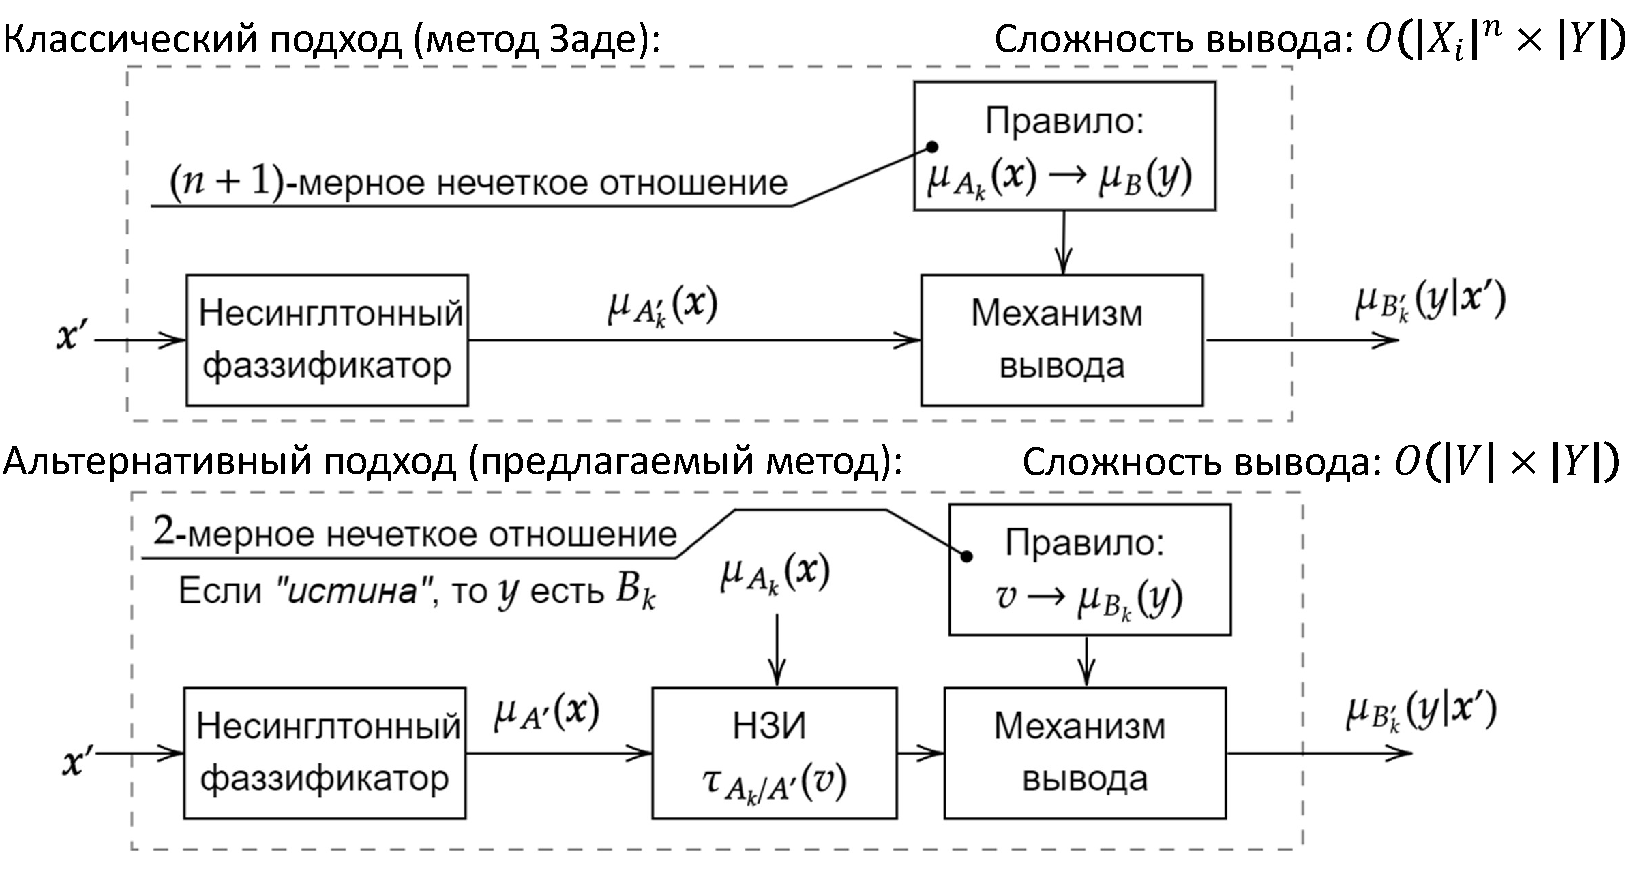
\includegraphics[scale=0.66]{ftv-schema-comparizon}
\caption{Сравнение классической схемы нечеткого вывода и схемы нечеткого вывода на основе НЗИ}
\label{fig:ftv-schema-comparizon}
\end{figure}

Порядок функции временной сложности вычисления $B'_k$ на основе выражения (\ref{eqn:ftv-compute-9}) составляет $O\left(n|V|^2+|V|\cdot |Y|\right)$, где $V=CP(A_k, A')$. Сравнение схем нечетких выводов с соответствии с соотношениями (\ref{eqn:fuz-problem-4}) и (\ref{eqn:ftv-compute-9}) представлены на рис. \cref{fig:ftv-schema-comparizon}.

\section{Вывод для систем логического типа}

\todo{\dots}
\todo{Выделяют следующие специальные категории импликаций:}
\todo{
\begin{itemize}
	\item S-импликация (Клине-Динеса, Лукасевича, Райхенбаха, Фодора): $I(a, b) = S(1-a, b)$
	\item R-импликация (Гогуен, Гедель): $I(a, b) = \sup_z \left\{z | T(a, z) \le b\right\}$
	\item Q-импликация (Заде, Вильмотта): $I(a, b) = S(1-a, T(a, b))$
\end{itemize}
}

В логическом подходе правила объединяются связкой <<И>>, тогда результирующее нечеткое множество является результатом произведения нечетких множеств, получаемых в результате нечеткого логического вывода по каждому правилу отдельно:

\begin{eqnarray}
B' = \CapOp_{r=1}^N B'_r.
\end{eqnarray}

\begin{equation}
\mu_{B'}(y) = \Tnorm_{r=1}^N \mu_{B'_r}(y) = \Tnorm_{r=1}^N \left\{\sup_{v\in [0, 1]} \left\{\tau_{A_r|A'}\overset{\mathrm{T}_2}{\star} I\left(v, \mu_{B_r}(y)\right)\right\}\right\}
\end{equation}

%Поскольку импликация в формуле (2.4)  не зависит от входных данных (\ref{eqn:2.2}), то предварительно, т.е. до использования композиционного правила (\ref{eqn:2.5}), вычисляется τ_(k,r) (v)=I(v,μ_(B_k ) (y ̅_r )) при k=(1,N) ̅,r=(1,N) ̅, v∈[0,1].



\section{Нечеткий вывод с использованием различных методов дефаззификации}

В статье \cite{VanLeekwijck1999} описывается подход к сравнению методов дефаззификации.

Описанный метод реализации \cite{eisele1994}.

\subsection{Дефаззификация по методу среднего центра}

%(center average)

\begin{equation*}
	\label{eqn:defuz-ca-1}
	\hat{y}_{CA} = \frac{\sum_{k=1}^{N} \bar{y}_k \mu_{B'_k}(\bar{y}_k)}{\sum_{k=1}^{N} \mu_{B'_k}(\bar{y}_k)}
\end{equation*}

\begin{figure}[ht]
	\centering
	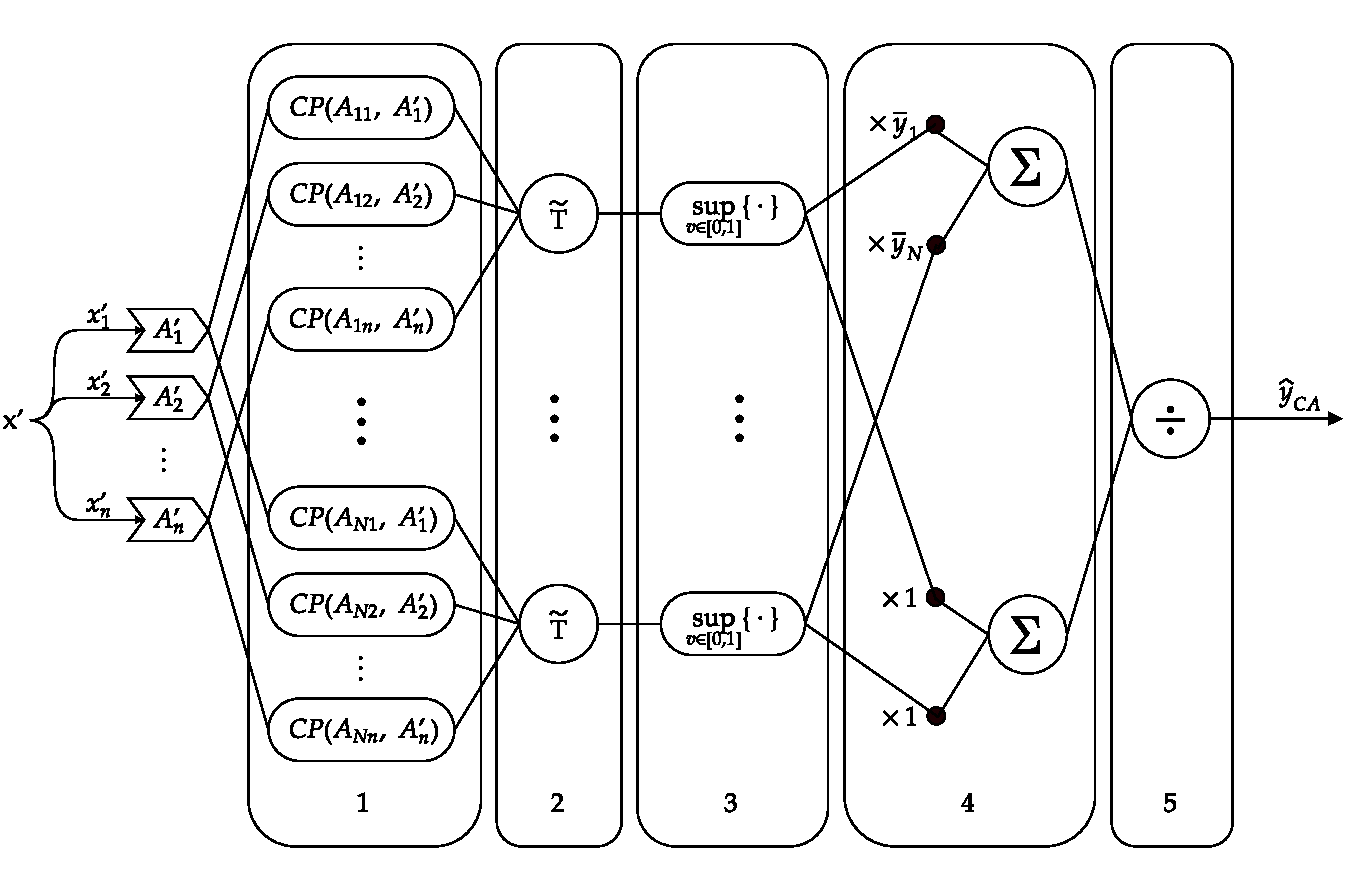
\includegraphics[scale=0.8]{neurofuzzysystem-defuzzification-ca-for-sr-impl}
	\caption{Схема нейро-нечеткой системы с использованием дефаззификации по методу среднего центра для $S$- и $R$-импликаций}
	\label{fig:neurofuzzysystem-defuzzification-ca-for-sr-impl}
\end{figure}

Поскольку $\mu_{B_r}(\overline{y}_k) = 1$ при $k = r$, тогда по формуле (\ref{eqn:ftv-compute-9}) $\mu_{B'_k}(\overline{y}_k)$ выразится:
\begin{align}
	\label{eqn:defuz-ca-3}
	\mu_{B'_k}(\overline{y}_k) &= \sup_{v\in [0, 1]} \left\{\tau_{A_k|A'}\overset{\mathrm{T}_2}{\star} I\left(v, \mu_{B_k}(\overline{y}_k)\right)\right\}\\ &= \sup_{v\in [0, 1]} \left\{\tau_{A_k|A'}\overset{\mathrm{T}_2}{\star} I\left(v, 1\right)\right\}.
\end{align}

Обозначив $I(v, 1) = I_1(v)$, с учетом () формула дефаззификации (\ref{eqn:defuz-ca-3}) примет вид:
\begin{equation}
	\label{eqn:defuz-ca-4}
	\hat{y}_{CA} = \frac{\sum_{k=1}^{N} \bar{y}_k \sup_{v\in [0, 1]} \left\{\tau_{A_r|A'}\overset{\mathrm{T}_2}{\star} I_1(v) \right\}}{\sum_{k=1}^{N} \sup_{v\in [0, 1]} \left\{\tau_{A_r|A'}\overset{\mathrm{T}_2}{\star} I_1(v) \right\}}
\end{equation}

Рассмотрим вычисление $\tau_k$ для различных категорий импликаций:
\begin{itemize}
	\item для \textit{S}-импликаций:
	\begin{align*}
		I_1(v) = I(v, 1) &= S\left\{1-a, 1\right\} = 1\\
	\end{align*}
	\item для \textit{R}-импликаций:
	\begin{align*}
		I_1(v) = I(v, 1) &= \sup_z \left\{z | T(v, z) \le 1\right\}&\quad v\in [0, 1]\\
		&= \sup_z \left\{z | \forall z\right\}&\quad z\in [0, 1]\\
		&= 1
	\end{align*}
	\item для \textit{Q}-импликаций:
	\begin{align*}
		I_1(v) = I(v, 1) &= S\left\{1-v, T(v, 1)\right\}\\
		&= S\left\{1-v, v\right\}\\
	\end{align*}
\end{itemize}


Тогда для \textit{S}- и \textit{R}-импликаций формула (\ref{eqn:defuz-ca-4}) с учетом свойства $t$-нормы $T(a, 1) = a$ примет вид:
\begin{align}
\hat{y}_{CA} &= \frac{\sum_{k=1}^{N} \bar{y}_k \sup_{v\in [0, 1]} \left\{\tau_{\mathbf{A_r}|\mathbf{A'}}\overset{\mathrm{T}_2}{\star} 1 \right\}}{\sum_{k=1}^{N} \sup_{v\in [0, 1]} \left\{\tau_{\mathbf{A_r}|\mathbf{A'}}\overset{\mathrm{T}_2}{\star} 1 \right\}}\\ &= \frac{\sum_{k=1}^{N} \bar{y}_k \sup_{v\in [0, 1]} \left\{\tau_{\mathbf{A_r}|\mathbf{A'}}\right\}}{\sum_{k=1}^{N} \sup_{v\in [0, 1]} \left\{\tau_{\mathbf{A_r}|\mathbf{A'}}\right\}},
\end{align}
а для \textit{Q}-импликации:
\begin{equation}
	\hat{y}_{CA} = \frac{\sum_{k=1}^{N} \bar{y}_k \sup_{v\in [0, 1]} \left\{\tau_{\mathbf{A_r}|\mathbf{A'}}\overset{\mathrm{T}_2}{\star} S\left\{1-v, v\right\} \right\}}{\sum_{k=1}^{N} \sup_{v\in [0, 1]} \left\{\tau_{\mathbf{A_r}|\mathbf{A'}}\overset{\mathrm{T}_2}{\star} S\left\{1-v, v\right\} \right\}}
\end{equation}

Схема нейро-нечеткого системы соответствующая формуле дефаззификации (\ref{}) изображена на рисунке \cref{fig:neurofuzzysystem-defuzzification-ca-for-sr-impl}.

\subsection{Дефаззификация по методу центра тяжести}

%(center of gravity)

Если выходное значение блока выработки решения представляет собой единственное агрегированное нечеткое множество $B'$, следует рассмотреть к использованию данный и последующие методы дефаззификации. Этот метод можно сопоставить со схемой вычисления математического ожидания случайной величины при данном ее распределении.

\begin{equation*}
\label{eqn:defuz-cog-1}
\hat{y}_{CoG} = \frac{\int_Y y \mu_{B'}(y) dy}{\int_Y \mu_{B'}(y) dy}
\end{equation*}

Тогда (\ref{}) при использовании данной импликации запишется в виде:
\begin{equation}
\hat{y}_{CoG} = \frac{\int_Y y \Tnorm_{r=1}^N \left\{sup_{v\in [0, 1]} \left\{\tau_{\mathbf{A_r}|\mathbf{A'}}\overset{\mathrm{T}_2}{\star} I\left(v, \mu_{B_r}(y)\right)\right\}\right\} dy}{\int_Y \Tnorm_{r=1}^N \left\{sup_{v\in [0, 1]} \left\{\tau_{\mathbf{A_r}|\mathbf{A'}}\overset{\mathrm{T}_2}{\star} I\left(v, \mu_{B_r}(y)\right)\right\}\right\} dy}
\label{eqn:defuz-cog-2}
\end{equation}

Значение $\hat{y}_{CoG}$ в данном способе дефаззификации может быть вычислено с применением численных методов. Однако существует упрощенная схема нахождения выходного значения в данном методе с помощью дискретной формулы центра тяжести в точках центров функций принадлежности термов выходной лингвистической переменной или ф. п. консеквентов правил в базе правил \cite{rutkovskiy2010}. Эта схема выражается формулой ниже.

\begin{equation}
\label{eqn:defuz-cog-3}
\hat{y}_{CoG} = \frac{\sum_{k=1}^{N} \overline{y}_k \mu_{B'}(\overline{y}_k)}{\sum_{k=1}^{N} \mu_{B'}(\overline{y}_k)},
\end{equation}
где $\overline{y}_k$ --- центр ф. п. нечеткого множества $B_k$, то есть такое значение $y$, в котором $\max_y \mu_{B_k}(y) = 1$.

В этом случае формула (\ref{}) на основе (\ref{}) примет вид:
\begin{align}
	\label{eqn:defuz-cog-4}
	\hat{y}_{CoG} = \frac{\sum_{k=1}^{N} \overline{y}_k \Tnorm_{r=1}^N \left\{sup_{v\in [0, 1]} \left\{\tau_{\mathbf{A_r}|\mathbf{A'}}\overset{\mathrm{T}_2}{\star} I\left(v, \mu_{B_r}(\overline{y}_k)\right)\right\}\right\}}{\sum_{k=1}^{N} \Tnorm_{r=1}^N \left\{sup_{v\in [0, 1]} \left\{\tau_{\mathbf{A_r}|\mathbf{A'}}\overset{\mathrm{T}_2}{\star} I\left(v, \mu_{B_r}(\overline{y}_k)\right)\right\}\right\}},
\end{align}

Выражение внутри фигурных скобок оператора $\sup_{v\in [0, 1]}\{\cdot\}$, представляющее композицию двух нечетких множеств на пространстве истинности, есть определение \textit{возможности}, то есть соответствие того, что $\tau_{\mathbf{A_r}|\mathbf{A'}}$ есть $\tau_{k\,r}$ и наоборот. Обозначим величину возможности:
\begin{equation}
	\sup_{v\in [0,1]}\left\{\tau_{\mathbf{A_r}|\mathbf{A'}}\overset{\mathrm{T}_2}{\star}\tau_{k\,r}\right\} = \Pi_{k\,r}
\end{equation}

Поскольку импликация в выражении (\ref(eqn:defuz-cog-4)) не зависит от входных данных, то значения $I(v, \mu_{B_r}(\overline{y}_k)) = \tau_{k\,r}, k=\overline{1,N}, r=\overline{1,N}$ могут быть вычислены предварительно, то есть до использования композиционного правила вывода.


\begin{figure}[ht]
	\centering
	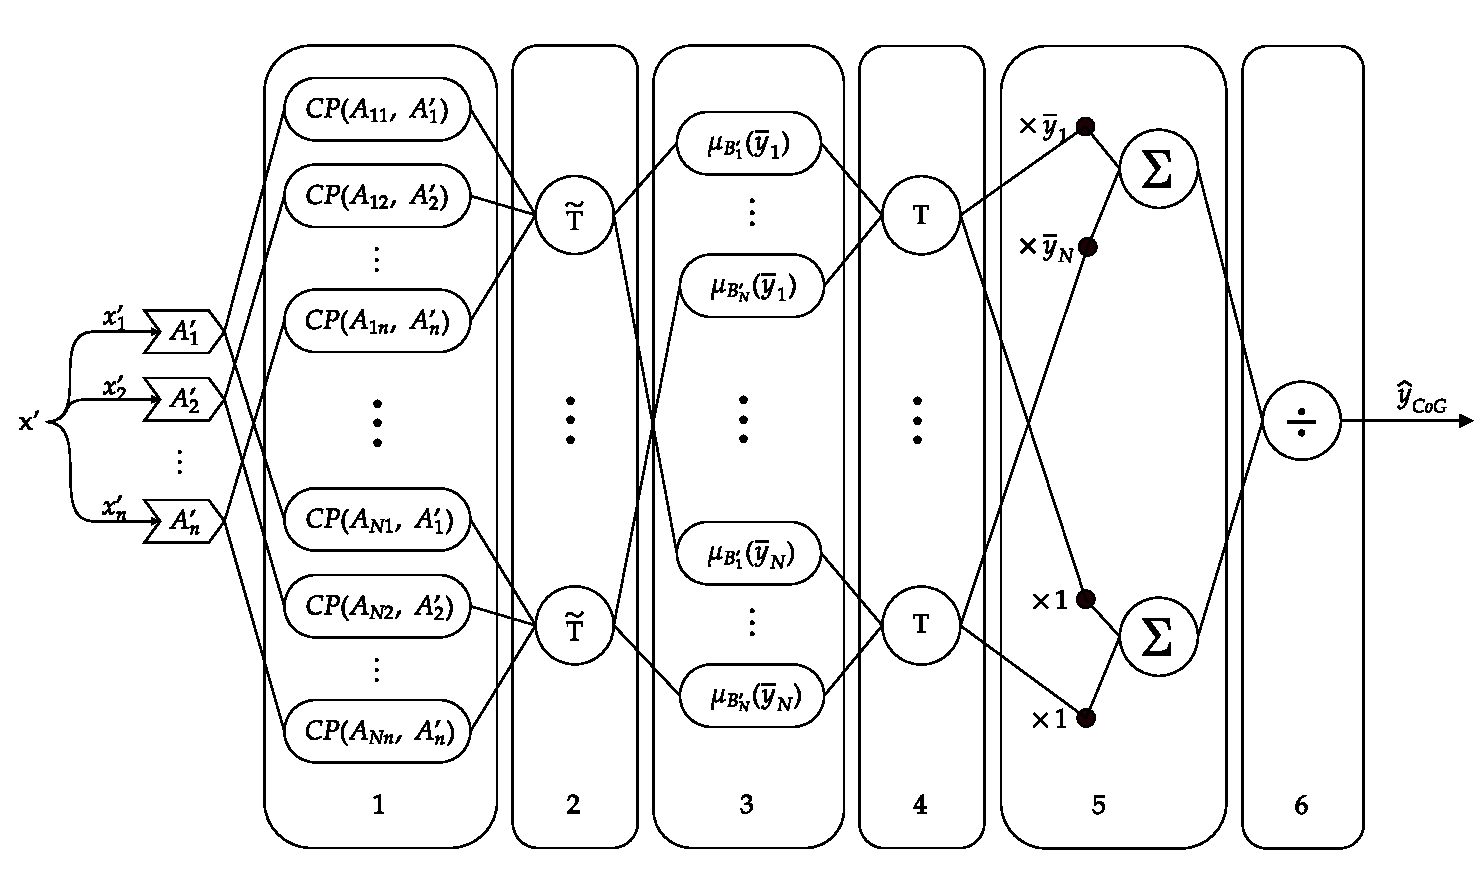
\includegraphics[scale=0.7]{neurofuzzysystem-defuzzification-cog}
	\caption{Схема нейро-нечеткой системы с использованием дефаззификации по методу центра тяжести}
	\label{fig:neurofuzzysystem-defuzzification-cog}
\end{figure}


\begin{figure}[ht]
	\centering
	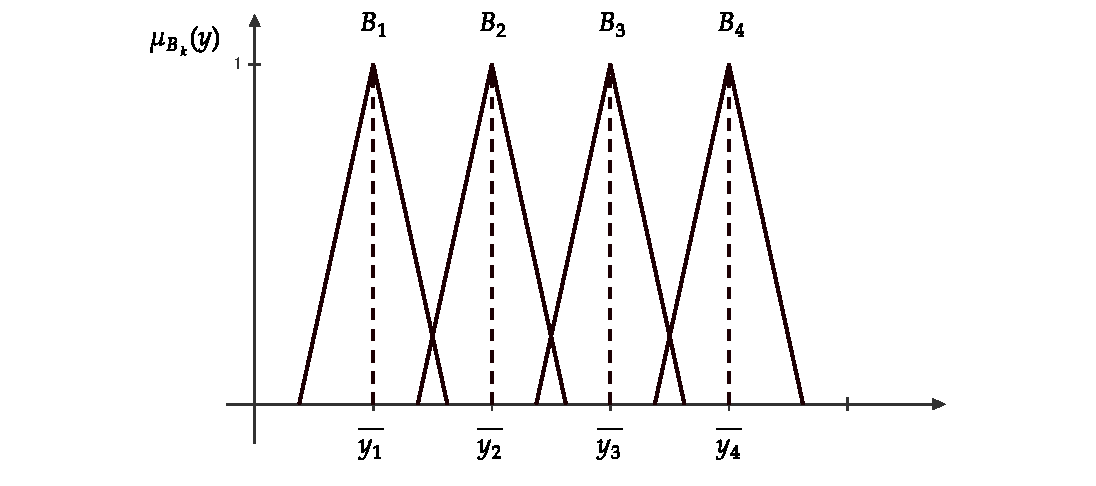
\includegraphics[]{out-mf-with-low-crossing}
	\caption{Пример нечетких множеств, удовлетворяющих условию $\mu_{B_k}(y_r) = 0$ для $y \ne r$}
	\label{fig:out_mf_with_low_crossing}
\end{figure}

Одна из возможностей упрощения процедуры вывода возникает, когда функции принадлежностей термов выходной лингвистической переменной достаточно удалены друг от друга и имеют низкую степень взаимного пересечения, то есть выполняется соотношение $\mu_{B_k}(y_r) \approx 0$ при $k \ne r$, что проиллюстрировано на рисунке \cref{fig:out_mf_with_low_crossing}.

Рассмотрим вычисление $\tau_{k\,r}$ для различных категорий импликаций:
\begin{itemize}
	\item для \textit{S}-импликации
	\begin{equation*}
		\tau_{k\,r}(v) = \begin{cases}
			1-v, & \quad \text{если } k \ne r \\
			1, & \quad \text{если } k = r
		\end{cases}
	\end{equation*}
	\begin{equation*}
		\hat{y}_{CoG} = \frac{\sum_{k=1}^{N} \overline{y}_k \Tnorm_{r=1}^N \left\{sup_{v\in [0, 1]} \left\{\tau_{A_r|A'}\overset{\mathrm{T}_2}{\star}(1-v)\right\}\right\}}{\sum_{k=1}^{N} \Tnorm_{r=1}^N \left\{sup_{v\in [0, 1]} \left\{\tau_{A_r|A'}\overset{\mathrm{T}_2}{\star}(1-v)\right\}\right\}},
	\end{equation*}
	\item для \textit{R}-импликации
	\begin{equation*}
	\tau_{k\,r}(v) = \begin{cases}
		\delta(v), & \text{если } k \ne r \\
		1, & \text{если } k = r
	\end{cases},
	\quad\text{где }
	\delta(v) = \begin{cases}
		1, & v = 0 \\
		0, & v > 0
	\end{cases}
	\end{equation*}
	\begin{equation*}
	\hat{y}_{CoG} = \frac{\sum_{k=1}^{N} \overline{y}_k \Tnorm_{r=1}^N \left\{\tau_{A_r|A'}(0)\right\}}{\sum_{k=1}^{N} \Tnorm_{r=1}^N \left\{\tau_{A_r|A'}(0)\right\}},
	\end{equation*}
	\item для \textit{S}-импликации
	\begin{equation*}
	\tau_{k\,r}(v) = \begin{cases}
		1-v, & \quad \text{если } k \ne r \\
		max(1-v, v), & \quad \text{если } k = r
	\end{cases}
	\end{equation*}
	\begin{equation*}
	\hat{y}_{CoG} = \frac{
		\sum_{k=1}^{N} \overline{y}_k \mathrm{T}_2 \left\{
			sup_{v\in [0, 1]} \left\{\tau_{A_k|A'}\overset{\mathrm{T}_2}{\star}max(1-v, v)\right\}
			\Tnorm_{\substack{r=1\\r\ne k}}^N \left\{
				sup_{v\in [0, 1]} \left\{\tau_{A_r|A'}\overset{\mathrm{T}_2}{\star}(1-v)\right\}
			\right\}
		\right\}
	}{
		\sum_{k=1}^{N} \mathrm{T}_2 \left\{
			sup_{v\in [0, 1]} \left\{\tau_{A_k|A'}\overset{\mathrm{T}_2}{\star}max(1-v, v)\right\}
			\Tnorm_{\substack{r=1\\r\ne k}}^N \left\{
				sup_{v\in [0, 1]} \left\{\tau_{A_r|A'}\overset{\mathrm{T}_2}{\star}(1-v)\right\}
			\right\}
		\right\}
	},
	\end{equation*}
\end{itemize}

\note{Можно организовать вычисление всех значений $b_{k\,r}$ $\tau_{k\,r}$, но использовать разреженные матрицы в качестве структуры данных для хранения значений где $b_{k\,r} > 0$.}

\note{Приведенные выклладки справедливы не только для функций принадлежностей отдельных термов, а и для набора кластеризованных в небольшие группы функций принадлжености со значительной степенью пересечения. При такой конфигурации выходного нечеткого пространства нет необходимости включать в процесс вывода правила, в которых функции принадлжености консеквента имеют низкий уровень пересечения с ф. п. правил, имеющих высокий уровень срабатывания для данного входа нечеткой системы.}

\subsection{Дефаззификация по методу центра области}

(center of area)

Данный метод можно сопоставить со схемой вычисления медианы случайной величины при заданном ее распределении. Формула вычисления дефаззифицированного значения $y^*_{CoA}$ имеет вид:

\begin{equation*}
\int_{\inf Y}^{\hat{y}_{CoA}} \mu_{B'}(y) dy = \int_{\hat{y}_{CoA}}^{\sup Y} \mu_{B'}(y) dy
\end{equation*}

\begin{align*}
\int_{\inf Y}^{\hat{y}_{CoA}} \Tnorm_{r=1}^N \left\{\sup_{v\in [0, 1]} \left\{\tau_{A_r|A'}\overset{\mathrm{T}_2}{\star} I\left(v, \mu_{B_r}(y)\right)\right\}\right\} dy =\\
= \int_{\hat{y}_{CoA}}^{\sup Y} \Tnorm_{r=1}^N \left\{\sup_{v\in [0, 1]} \left\{\tau_{A_r|A'}\overset{\mathrm{T}_2}{\star} I\left(v, \mu_{B_r}(y)\right)\right\}\right\} dy
\end{align*}

\subsection{Дефаззификация по методу среднего максимума}

\begin{equation*}
\hat{y}_{MeOM} = \frac{\sum_{x \in core(B')} x}{|core(B')|},
\end{equation*}
где $core(B') = \left\{y | y \in Y \textrm{ and } \mu_{B'}(y) = \sup_{y' \in Y} \mu_{B'}(y')\right\}$. 

Данный метод аналогичен по схеме вычисления моде случайной величины при заданном ее распределении. В случае унимодального вида функции принадлежности $\mu_{B'}(y)$ данный способ дефаззификации можно упростить до метода максимума функции принадлежности:
\[
\hat{y}_{MeOM} = \mathrm{arg\,max}_{y \in Y} \mu_{B'}(y).
\]

Тогда 
\begin{equation}
	\hat{y}_{MeOM} = \arg\,\max_{y\in Y} \Tnorm_{r=1}^N \left\{\sup_{v\in [0, 1]} \left\{\tau_{A_r|A'}\overset{\mathrm{T}_2}{\star} I\left(v, \mu_{B_r}(y)\right)\right\}\right\}
\end{equation}


\section{Классификация объектов на основе нечеткого вывода с использованием нечеткого значения истинности}

Описанная в разделе \cref{sec:ch2/ftv-based-inference-statement} нечеткая система в общем случае используется для моделирования. Тогда, можно использовать этот логический вывод для определения принадлежности некоторого объекта к каждому из заданного множества классов, т. е. с помощью этой нечеткой системы можно решать задачу многоклассовой классификации.

В классических методах классификация производится для данного объекта $q$ с набором значений атрибутов, каждый из которых формализуется числовым значением признака. В случае использовании для этого нечеткой системы, значения признаков формализуются посредством термов лингвистических переменных $\mathbf{x}=[x_1,\dots,x_n ]$, совокупность значений которых формирует вектор $\mathbf{A'}=\left[A'_1,A'_2,\dots,A'_n\right]$, что соответствует посылке:
\begin{equation*}
	\langle x_1\text{ есть }A'_1\text{ и }x_2\text{ есть }A'_2\text{ и }\dots \text{ и }x_n\text{ есть }A'_n\rangle
\end{equation*}

При этом рассмотренный выше метод нечеткого вывода позволяет обрабатывать значения признаков объекта, заданные с использованием фаззификации типа non-singleton, учитывающей зашумленность значений этих признаков.

%Например, значение лингвистической переменной может быть задано нечетким множеством, характеризующегося гауссовой функцией принадлежности. В этой функции значение мат ожидания равно значению признака объекта, а среднеквадратичное отклонение – совпадает с среднеквадратичным отклонением всего набора объектов, принадлежащих данному классу.

Пусть классификация производится для множества из $m$ классов $\Omega=\left\{\omega_1,\dots,\omega_m\right\}$. Тогда база знаний нечеткой систем описывается набором из $N$ правил вида:

\begin{equation}
	\begin{aligned}
	R_k: \textrm{Если }&x_1\textrm{ есть }A_{k1}\textrm{ и }x_2\textrm{ есть }A_{k2}\textrm{ и }\dots\textrm{ и } x_n\textrm{ есть }A_{kn},&\\
	\textrm{ то }&q_k \in \omega_1 (\bar{z}_{k1})\textrm{ и }q_k \in \omega_2 (\bar{z}_{k2})\textrm{ и }\dots\textrm{ и }q_k \in \omega_m (\bar{z}_{km}), k \in \overline{1,N},
	\end{aligned}
	\label{eqn:fuzzy-classify-1}
\end{equation}

где $z_{kj}$ --- степень принадлежности объекта $q$ к классу $\omega_j$ в соответствии с правилом $R_k$. Значения $\bar{z}_{kj}$ могут быть определены при помощи метода парных сравнений \cite{} на основании набора объектов-образцов $Q = \left\{q_k\right\}_{k=1}^N$. Каждому значению $z_{kj}$ можно поставить в соответствие значение лингвистической переменной $z_j$, которое выражается нечетким множеством $B_{kj}$ имеющим в качестве базового множеств диапазон $[0, 1]$, обозначающий вероятность принадлежности объекта к $j$-му классу.

В случае, если база правил представляет собой набор эталонных объектов процедура нечеткого вывода может быть упрощена за счет использования в качестве термов выходных лингвистических переменных синглтонных нечетких множеств $B_{k1}, B_{k2}, \dots, B_{km}$ c функцией принадлежности:
\begin{equation*}
	\mu_{B_{kj}}(z_j) = \begin{cases}
		1, \quad&\text{если } z_j = \bar{z}_{kj},\\
		0, \quad&\text{если } z_j \ne \bar{z}_{kj}.
	\end{cases}
\end{equation*}	

Тогда, согласно (\ref{}):
\begin{equation*}
	1
\end{equation*}

Принадлежность объекта к одному из $m$ классов затем определяется по формуле:
\[
	j^* = \argmax_{j=\overline{1,m}} \hat{z}_j,
\]
где $\hat{z}_j$ --- дефаззифицированное значение выходной лингвистической переменной $z_j$.

Если задача мультиклассовой классификации позволяет отнесение объекта сразу к нескольким классам, окончательное решение может быть получено на основании условий:
\begin{equation*}
	\begin{cases}
		q \in \omega_j, \quad&\text{если }\hat{z}_j \geq z_{inc},\\
		q \notin \omega_j, \quad&\text{если }\hat{z}_j \leq z_{exc},\\
		\text{не определено}, \quad&\text{если }z_{exc} < \hat{z}_j < z_{inc},
	\end{cases}
\end{equation*}
где числа $z_{inc}$ и $z_{exc}$ --- фиксированные пороговые значения, такие, что:
\[
	0 \leq z_{exc} \leq z_{inc} \leq 1.
\]

%В этом правиле степень принадлежности объекта $q$ к классу $\omega_j$ задается  значением $(z_{kj})$, которому можно поставить в соответствие значение лингвистической переменной $z_j$. Это значение выражается нечетким множеством имеющим в качестве базового множеств диапазон $[0,1]$ вероятности принадлежности объекта к заданному классу.

%Тогда, правило \ref{eqn:fuzzy-classify-1} можно переписать в виде, в котором было записано правило (1) для системы нечеткого вывода, заменив при этом лингвистические переменные y_j на z_j, где j=(1,m) ̅.
%R_k:Если x_1  есть A_1k  и x_2  есть A_2k  и,…,и x_n  есть A_nk,
%то z_1  есть B_1k  и z_2  есть B_2k  и… и z_m  есть B_mk.


\section{Прогнозирование временных рядов на основе нечетких систем логического типа с использованием нечеткого значения истинности}

Определив НЗИ $CP(\mathbf{A_{k}, \mathbf{A'}})$ для антецедента правила $R_k$ согласно (\ref{eqn:ftv-compute-12}) и (\ref{eqn:ftv-compute-8}), можно переписать правило $R_k$ в виде:
\begin{align*}
	R_k: \textrm{Если }&CP(\mathbf{A_{k}, \mathbf{A'}}),&\\
	\textrm{ то }&y_{t+1}\textrm{ есть }A_{k\,p+1},&k\in\overline{1,N}.
\end{align*}

\todo{Вычисленное значение истинности для каждого правила выражает соответствие среза измерений порождаемых некоторым величины некоторой единице знаний о динамике этого процесса.}

Если используется логический метод вывода на основе дефаззификации по центру тяжести, то согласно (\ref{}) нечеткий вывод выражается:
\begin{equation}
\hat{y}_{t+1} = \frac{\int_Y y_{t+1} \underset{k=\overline{1,N}}{\textrm{T}}\Biggl\{\sup_{v \in [0,1]}\biggl\{\tau_{\mathbf{A_k}|\mathbf{A'}}(v)\overset{T_2}{\star} I(v, \mu_{A_{k\,p+1}}(y_{t+1}))\biggr\}\Biggr\} dy_{t+1}}{\int_Y \underset{k=\overline{1,N}}{\textrm{T}}\Biggl\{\sup_{v \in [0,1]}\biggl\{\tau_{\mathbf{A_k}|\mathbf{A'}}(v)\overset{T_2}{\star} I(v, \mu_{A_{k\,p+1}}(y_{t+1}))\biggr\}\Biggr\} dy_{t+1}}
\end{equation}



\section{Выводы}

\begin{enumerate}
	\item С использованием нечеткого значения истинности можно построить альтернативный метод нечеткого логического вывода. Данный метод соответствует каноническому логическому выводу Заде за счет эквивалентного преобразования пространства антецедента правил. Преобразование истинностной модификации отображает многомерное пространство антецедента в одномерное пространство истинности, из-за чего база правил приобретает новую структуру правил вида: <<Если \textit{истинно}, то $B_k$>>. Вычисление посылки нечеткого значения истинности составляет предшествующий непосредственно логическому выводу этап, и формируется из нахождения НЗИ между нечетким множеством в антецеденте и входной посылки по каждому входу отдельно и последующей свертки в единое пространство НЗИ с помощью расширенной $t$-нормы --- $\tilde{\mathrm{T}}$.
	\item Для предложенного метода нечеткого вывода применимы различные способы дефаззификации выходного значения. \note{Схема вычисления дефаззификации по методу среднего центра значительно упрощается. Вычисление дефаззификации по упрощенной схеме сводится к нахождению величины меры возможности $1$. В случае, когда нечеткие множества удалены друг от дурга и имеют низкую степень взаимного пересечения итоговые формулы дефаззификации упрощаются за счет.} \todo{Это позволяет\dots}
	\item Показано как \dots применен для решения задач классификации объектов с нечеткими атрибутами и для прогнозирования временных рядов.
\end{enumerate}

\todo{Проведен анализ\dots}

\todo{В главе приведены итоговые формулы нечеткого вывода на основе нечеткого значения истинности для различных методов дефаззификации. Также выведены упрощенные формулы вычисления дефаззифицированного значения для различных специальных категорий импликаций.}

\todo{Дано формальное описание применения разработанной модели нечеткого логического вывода в задаче прогнозирования временных рядов. Приведены существующие подходы фаззификации значений временных рядов и методы автоматического подбора параметров термов лингвистической переменной и формирования базы правил на основе наборов обучающих данных.}

\FloatBarrier
           % Глава 2
\chapter{Программая реализация разработанного метода нечеткого вывода с применением технологии CUDA}\label{ch:ch3}

Для удобства реализация выполнялась не постредством прямого использованием API библиотеки CUDA, а с помощью шаблонной библиотеки реализации высокопроизводительных вычислений - \textbf{Kokkos} \ref{}, предназначенной для портативного и эффективного параллельного программирования на различных аппаратных архитектурах, включая многоядерные процессоры, графические процессоры NVIDIA/AMD и другие ускорители. Интерфейс библиотеки позволяет абстрагироваться от деталей низкоуровневого параллелизма, позволяя разработчикам писать код на C++ с одним исходным кодом, который может быть оптимизирован для различных платформ без существенных изменений. 
Ключевые функциональные возможности библиотеки упростившие выполнение программного реализации разработанного ранее метода:
\begin{itemize}
\item Модели параллельного выполнения: абстрагирование параллельных циклов (например, "parallel\_for", "parallel\_reduce") и рабочих процессов на основе задач.  
\item Управление памятью: Автоматизированная обработка пространств памяти (например, между хостом и устройством) и расположением данных для оптимизации схем доступа и минимизации объема передаваемых данных.  
\item Поддержка серверной части: интеграция с такими моделями программирования, как CUDA, HIP, OpenMP и SYCL, для обеспечения кроссплатформенной совместимости.  
\item Переносимость производительности: Обеспечивает эффективное использование ресурсов (потоки, векторизация) с учетом особенностей каждой архитектуры.
\end{itemize}

Kokkos широко используется в научных вычислениях и HPC-приложениях, упрощая разработку масштабируемых кодов при сохранении производительности на постоянно развивающемся оборудовании. 

При выполнении процедуры нечеткого вывода для набора входных данных можно выполнять процедуру вывода по каждому входному экземпляру независимо, то есть параллельно. Кроме того можно предусмотреть отбор небольшого в сравнении с общим количеством ограниченного подмножества правил нечеткой системы, наиболее релевантных входному экземпляру. Сам алгоритм нечеткого вывода не предусматривает наличия промежуточной информации, котой бы нужно было обмениваться между вычислениями по другим экземплярам входных данных. Тогда, поскольку алгоритм нечеткого вывода для каждого экземпляра входных данных можно реализовать при ограниченном небольшом объеме входных и промежуточных данных, имеет смысл разместить эти данные в памяти предоставляющей наибольшую скорость обращения, которая в технологии CUDA соответствует динамической памяти внутри CUDA-блока, а сами вычисления над этими данными также реализовать внутри этого CUDA-блока.



\section{Вычисление нечеткого значения истинности с помощью дискретизации функций принадлежностей}\label{sec:ch3/sect1}

\begin{figure}[hbt]
	\centering
   	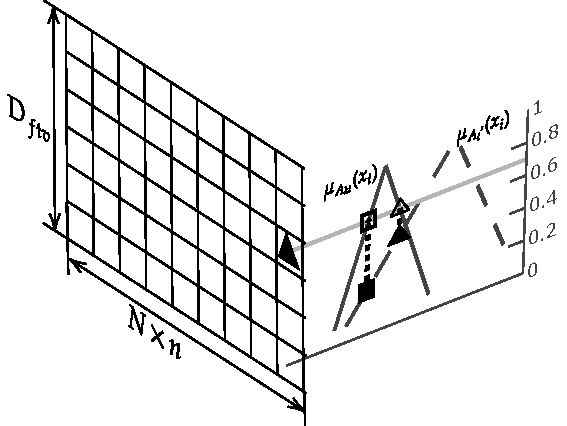
\includegraphics[width=0.6\textwidth]{ftv-opengl-computation.pdf}
	\label{ftv-opengl-computation}
\end{figure}

\begin{figure}[hbt]
	\centering
   	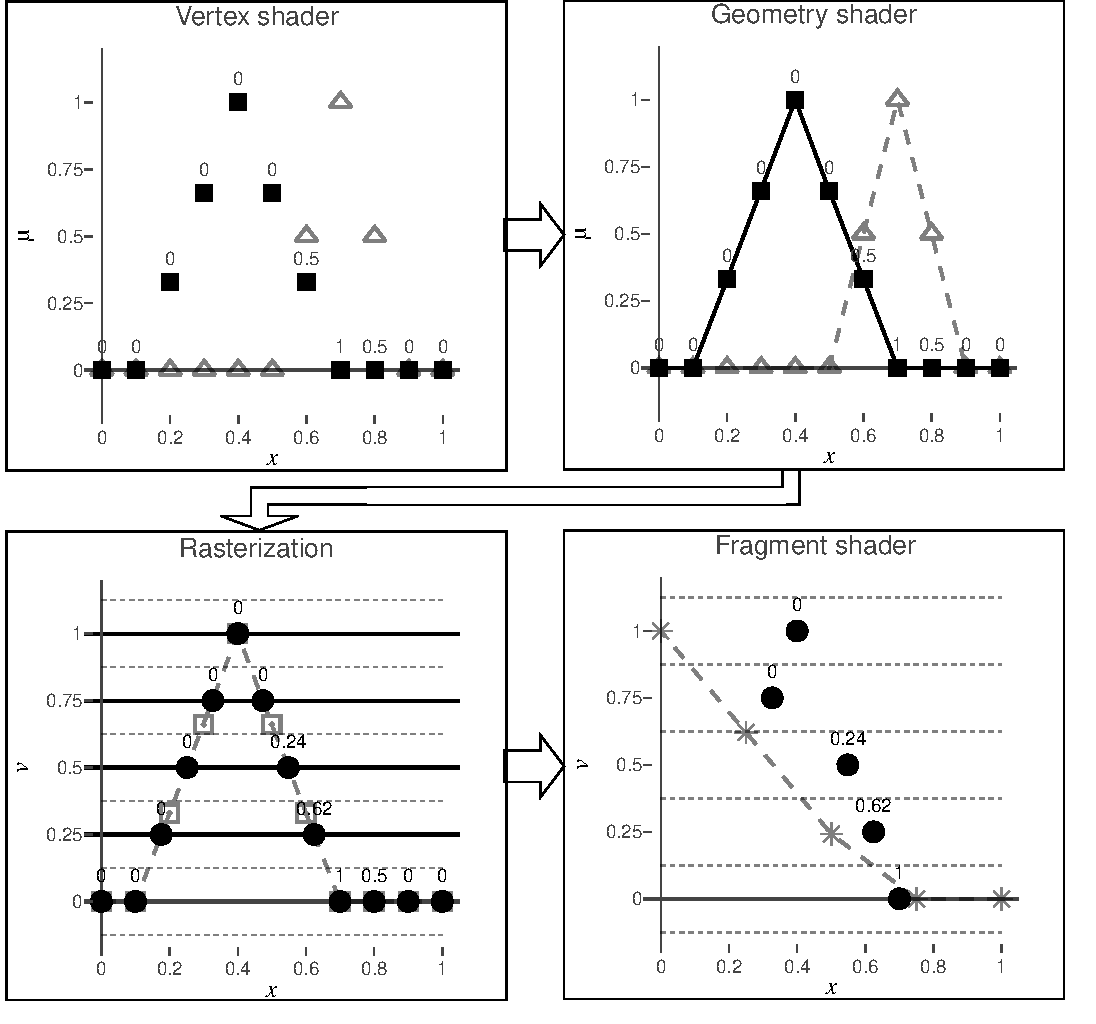
\includegraphics[width=1.0\textwidth]{ftv-opengl-computation-pipeline.pdf}
	\label{ftv-opengl-computation-pipeline}
\end{figure}

\section{Алгоритм свертки НЗИ при $T_1=min$ и $T_3$ - неубывающая по всем аргументам}\label{sec:ch3/sect2}

\begin{algorithm}
\label{alg:ftv-reduction}
\begin{algorithmic}
\Require $ftv_i,\ i=\overline{1,n}$
\State $max\_ftv[i] = 0;$
\For{$v = 1\dots0$}
\State $s \gets \left\{ftv_i[v] \mid ftv_i[v] >= max\_ftv[i]\right\};$
\State $max\_ftv[i] \gets max(max\_ftv[i], ftv_i[v]);$
\State $v\_max \gets \max_{i}\left\{ftv_i[v]\right\}, v\_max\_index \gets \mathrm{arg\,max}_i\left\{ftv_i[v]\right\};$
\If{$s = \emptyset \And i = v\_max\_index$}
\State $r[i] \gets v\_max;$
\Else
\State $r[i] \gets max\_ftv[i];$
\EndIf
\State $ftv[v] \gets \underset{i}{T_3}\left\{r[i]\right\}$;
\EndFor
\State \Return $ftv$
\end{algorithmic}
\caption{Алгоритм свертки НЗИ при $T_1=min$ и $T_3(a, b) \ge T_3(c, d)$ если $a > c$ или $b > d$}
\end{algorithm}

\begin{figure}
    \label{fig:ftvs-reduction-example}
    \centering
    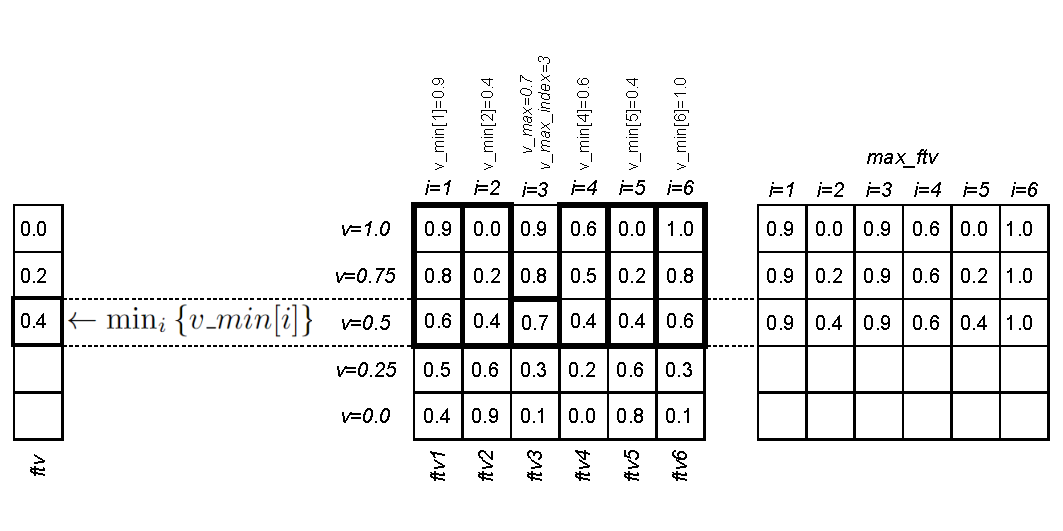
\includegraphics[width=15cm]{ftvs-reduction-example.pdf}
    \caption{Иллюстрация работы алгоритма свертки НЗИ для нескольких входов для расширенной $\mathrm{\tilde{T}}$-нормы при $T_1=\mathrm{min}$ и $T_3=\mathrm{min}$.}
\end{figure}

При 

\pgfplotsset{
    axis grid/.style={
        width=0.3\textwidth,
        height=0.3\textwidth,
        domain=0:1,
    }
}

\begin{figure}
	\centering
	\begin{tikzpicture}[
	    % Style for column headers (above each column)
	    column header/.style={
	        anchor=south,
	        font=\bfseries,
	        yshift=10pt
	    },
	    % Style for row headers (left of each row)
	    row header/.style={
	        anchor=east,
	        font=\bfseries,
	        xshift=-10pt,
	        rotate=90
	    }
	]
		\matrix[row sep=0.5cm, column sep=0.1cm] (mat) {
			\node[] {}; &
			\node[column header] {$\tau_{A_k|A'} =$ <<АБСОЛЮТНО ЛОЖНО>>}; &
			\node[column header] {Column 1}; &
			\node[column header] {Column 1}; \\
			
			\node[row header] {$\mu_{B_k}(y) = 0$}; &
			\begin{axis}[axis grid]
				\addplot {(1-x)^2};
			\end{axis} &
			\begin{axis}[axis grid]
			\end{axis} &
			\begin{axis}[axis grid]
			\end{axis} \\
		};
	\end{tikzpicture}
\end{figure}

\section{Реализация дефаззификации}

Нахождение начального приблежения

\section{Использование библиотеки ArborX}\label{sec:ch3/sect2}

\begin{figure}[hbt]
	\label{fig:z-curve-apetrei}
	\centering
	\begin{minipage}[b]{0.45\textwidth}
		\centering
		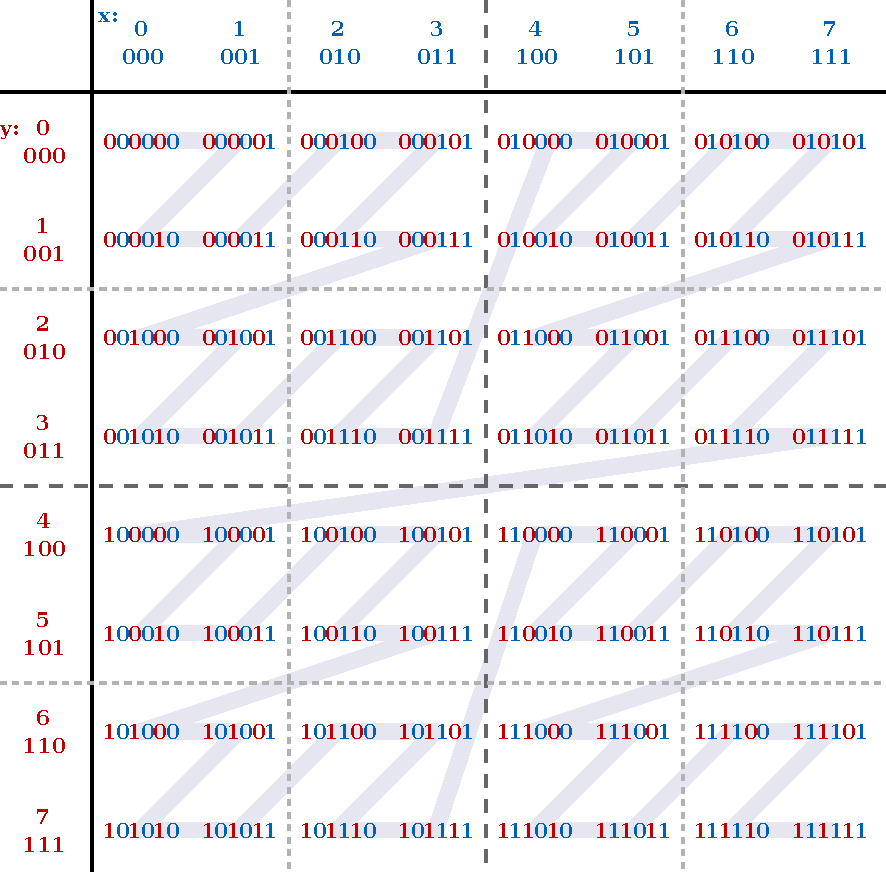
\includegraphics[width=\textwidth]{z-curve}
		\caption*{(a) z-curve}
	\end{minipage}\hfill
	\begin{minipage}[b]{0.45\textwidth}
		\centering
		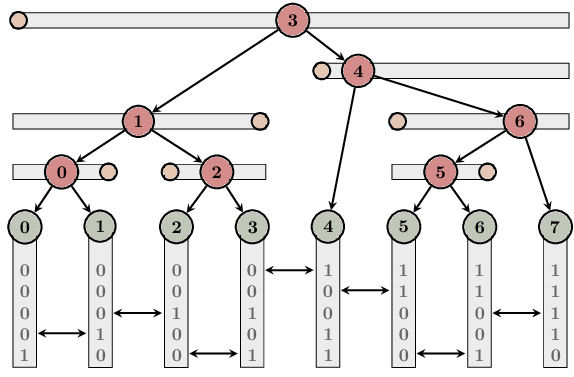
\includegraphics[width=\textwidth]{apetrei}
		\caption*{(b) apetrei}
	\end{minipage}
	\caption{Две иллюстрации: графика z-curve и apetrei.}
\end{figure}

В \cite{prokopenko2024revisingapetreisboundingvolume} авторами библиотеки \textbf{ArborX} предложен алгоритм для эффективного построения \textit{иерархии ограничивающих объемов}. Данная структура данных используется для эффективного поиска ближайшей точки в $n$-мерном пространстве. Алгоритм выполняет построение структуры поиска за $O(N\times log(N))$, где $N$ - количество точек в исходном наборе. Логика поиска места в иерархии ограничивающих объемов для каждой отдельной точки помещена в отдельную нить параллельных вычислений, после чего остается ятолько логирифмическая компонента сложности, соответствующая восходящему обходу промежуточного дерева и помещения точки в подобранный узел \fixme{с использованием атомарной операции}. В основе алгоритма лежит группировка близко расположенных точек для более быстрого подбора соответствующего ограничивающего объема за счет проецирования точки из $n$-мерного пространства на $Z$-кривую посредством вычисления кода Мортона для каждой точки. Согласно эвристике, лежащие рядом на $Z$-кривой точки располагаются достаточно близко и исходном $n$-мерном пространстве. Кроме того в статье описан модифицированный алгоритм Апетрея [], обеспечивающий обход иерархии на этапе поиска ближайших точек без необходимости помещения цепочки пройденных родительских узлов в стек за счет передачи информации об альтернативных узлах-кандидатах из родительских узлов в дочерние. Такой подход значительно снижает количество потребляемой памяти для сохранения промежуточной информации при выполении этапа поиска.

\section{Алгоритм построения базы правил}

           % Глава 3
\chapter{Применение разработанной нечеткой модели для прогнозирования временных рядов в задачах экономики и финансов}

Прогнозирование временных рядов в экономике и финансах играет ключевую роль как инструмент анализа и предсказания динамики последовательно изменяющихся данных. Оно служит основой для принятия обоснованных решений в условиях неопределенности, обеспечивая оценку будущих тенденций, рисков и возможностей. Это позволяет субъектам экономической и финансовой деятельности — от индивидуальных инвесторов до государственных структур — оптимизировать управление ресурсами, минимизировать потери и формировать долгосрочные стратегии.

Стратегическое планирование и бюджетирование (обоснование финансовых планов, оптимизация ресурсного распределения), Управление рисками и инвестиционные решения

В государственных и корпоративных бюджетах прогнозы временных рядов используются для оценки объёмов доходов и расходов, планирования денежных потоков и определения ключевых показателей эффективности. У компаний прогнозирование сезонных и трендовых колебаний продаж помогает корректировать производственные мощности, склады и персонал, тем самым минимизируя издержки и снижая риск дефицита или перепроизводства. Прогнозы временных рядов служат основой для разработки моделей оптимального распределения активов и стратегий ребалансировки портфеля в зависимости от ожидаемых рыночных движений.

Одномерные модели оправданы, когда целевой ряд обладает высокой автокорреляцией, слабо зависит или отсутствует информация о значениях внешних факторов, ограниченны вычислительные и временные ресурсы для оценки взаимосвязей измерений. Примеры: краткосрочное прогнозирование инфляции, прогнозирование индекса S\&P 500. Многомерные методы необходимы, когда влияние других временных рядов или внешних предикторов существенно для точности прогноза, доступна качественная информация об этих переменных или когда доступна информация о их будущих значениях, а также когда необходимо исследовать влияние <<шока>> в одной переменной на остальные. Примеры: оценка влияния нефтяных шоков на экономику Нигерии.

\todo{Область и ситуации в которой применима разработанная модель (авторегрессионная)}

\todo{Для прогнозирования используются модели}

\section{Задача прогнозирования стоимости ценных бумаг Тайванской биржи}

\cite{Sadaei2016}

Taiwan Capitalization Weighted Stock Index (TWSE) - популярный набор данных стоимости акций биржи TAIEX, исполюзуемый для оценки качества прогнозирования временных рядов. Датасет предоставляется официальным сайтом  Набор данных составлен из ежедневных значений цены индекса в момент закрытия биржи в промежутке от 2001 до 2022 года.

\begin{figure}[hbt] 	
	\label{fig:twse-ns-fuzzification}
	\centering
	%\includegraphics[width=\textwidth]{twse-ns-fuzzification}
	\caption{Тренировочный и тестовый отрезок значений временного ряда TWSE и среднеквадратичное отклонение гауссовой ф. п. в каждой точке.}
\end{figure}

 Для оценки качества были отложены последние 500 окон временных точек, а для построения базы правил использовались предшествующие им 1000 окон. Отрезки исходного временного ряда для тестовый и тренировочный выбирались таким образом, чтобы диапазон значений в тестовом отрезке был включен в диапазон тренировочного отрезка. Фаззификация временного ряда состояла в построении гауссовой функции принадлежности в каждой точке временного ряда. Центры гауссовой функции принадлежности равны значениям временного ряда в каждой точке. Значение среднеквадратичного отклонения находится согласно способу описанному в разделе \ref{} главы \ref{}: \todo{уточнить}.
 
 \begin{figure}[hbt] 	
 	\label{fig:twse-optuna-parallel-score}
 	\centering
 	%\includegraphics[width=\textwidth]{twse-optuna-parallel}
 	\caption{Влияние комбинации значений гиперпараметров на значение оптимизируемой метрики.}
 \end{figure}
 
В рамках данной задачи горизонт прогнозирования задается равным 1. В качестве функции приспособленности использовалась метрика \todo{NDEI}.

Для оценки предельных возможностей непосредственно нечеткой логической модели в данной задаче параметры $\alpha,\dots$ подбирались с помощью байесовской оптимизации, реализованной в Python-библиотеке Optuna \cite{Optuna2024, akiba2019optuna}. \todo{Диапазоны значений этих параметров, в пределах которых производился поиск оптимальной комбинации, приведены в таблице}. Для сокращения длительности байесовой оптимизации размер популяции выбирался равным количеству правил в базе правил, а число итераций ролевого алгоритма подбора базы правил --- 50. Для алгоритма Gradient-aware PSO в методе дефаззификации MeOM размер популяции составляет 30 особей, а количество итераций --- 100. График значений оптимизируемой метрики для различных комбинаций значений гиперпараметров нечеткой модели в параллельных координатах изображен на рисунке \cref{fig:twse-optuna-parallel-score}. Из него можно отметить несколько наблюдений. При значение параметра лага $p = 5$, значении коэффициента среднеквадратичного отклонения функций принадлежности для фаззифицированных входных данных $\phi = 0.1$ и количестве правил в базе правил $N = 50$ обеспечивается лучшее значение целевой метрики. Также лучшее качество прогнозирования на тренировочном отрезке временного ряда достигается при использовании нечеткой импликации \textit{Лукасевича} и метода дефаззфикации --- \textit{MeOM}.

\begin{figure}[hbt] 	
	\label{fig:twse-optuna-parallel-duration}
	\centering
	%\includegraphics[width=\textwidth]{twse-optuna-parallel}
	\caption{Влияние комбинации значений гиперпараметров на время построения базы правил.}
\end{figure}

На рисунке \cref{fig:twse-optuna-parallel-duration} график изображает зависимость времени оптимизации базы правил нечеткой системы при тех же комбинациях гиперпараметров, что и на рисунке \cref{fig:twse-optuna-parallel-score}.

\begin{figure}[hbt] 	
	\label{fig:twse-rules-pso-optimization}
	\centering
	%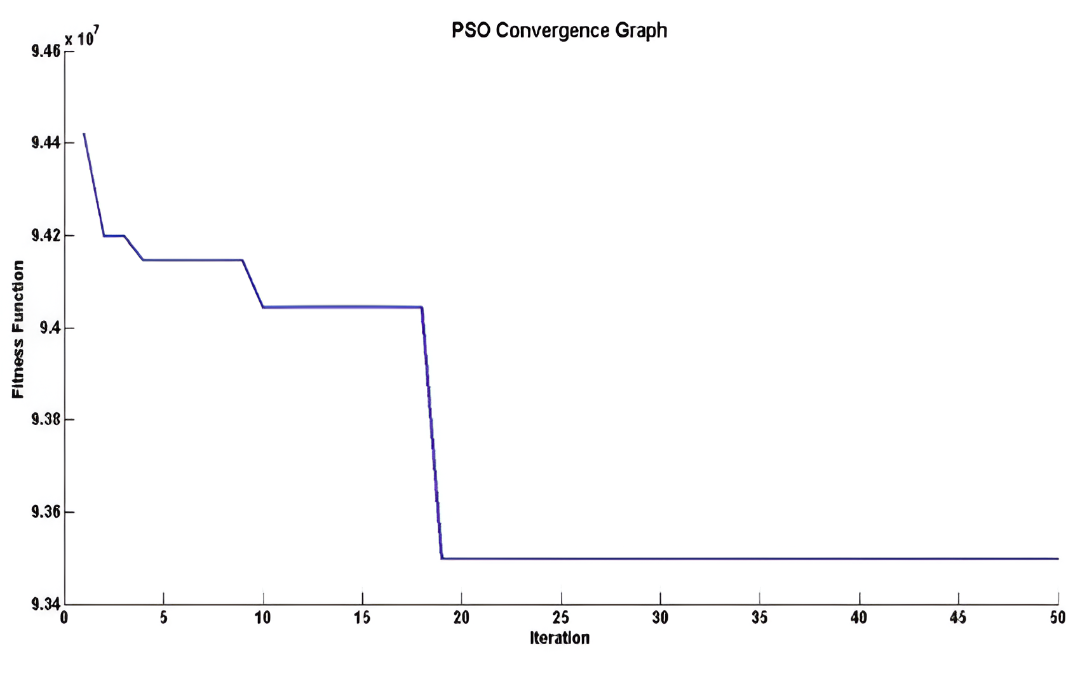
\includegraphics[width=\textwidth]{twse-rules-pso-optimization}
	\caption{Графики изменений максимального, среднего и лучшего по популяции значений оптимизируемой метрики.}
\end{figure}

Динамика максимального, среднего и лучшего по популяции значений оптимизируемой метрики в процессе PSO-оптимизации базы правил для подобранной выше комбинации гиперпараметров изображена на рисунке \cref{fig:twse-rules-pso-optimization}.

\begin{table} [htbp]% Пример записи таблицы с номером, но без отображаемого наименования
	\caption{Сравнение показателей качества прогнозирования временного ряда из набора данных TWSE (TAIEX).}%
	\label{tab:test1}%
	\begin{SingleSpace}
%			\begin{tabular}{| c{5cm} | *{2}{C{2.5cm}} | l *{3}{C{1.5cm}} |}
     \setlength\extrarowheight{2pt} %вот этим управляем расстоянием между рядами, \arraystretch даёт неудачный результат
\setlength{\tymin}{1.5cm}% минимальная ширина столбца
     \begin{tabulary}{\textwidth}{@{}>{\zz}C >{\zz}C >{\zz}C >{\zz}C >{\zz}C >{\zz}C@{}}% Вертикальные полосы не используются 	принципиально, как и лишние горизонтальные (допускается по ГОСТ 2.105 пункт 4.4.5) % @{} позволяет прижиматься к краям
			\toprule
			\multirow{2}{*}{Модель} & Время обучения, сек. & Время вывода, сек. & RMSE & MAPE & MAE \\
			\midrule
			MLP & -- & -- & 7.93     & 8.77     & 8.77     \\
			Decision Tree & -- & -- & 8.77     & 8.77     & 8.77     \\
			SVM & -- & -- & 8.77     & 8.77     & 8.77     \\
			ANFIS (Мамдани) & -- & -- & 8.77     & 8.77     & 8.77     \\
			ANFIS (Такаги-Сугено) & -- & -- & 8.77     & 8.77     & 8.77     \\
			\hline
			FTV-NSFLS+COG (упрощенная схема)        & 8.72     & 8.77     & 8.77     & 8.77     & 8.77     \\
			FTV-NSFLS+MeOM        & 8.72     & 8.77     & 8.77     & 8.77     & 8.77     \\
			\bottomrule
		\end{tabulary}%
	\end{SingleSpace}
\end{table}

\begin{figure}
	\centering
	%\includegraphics[scale=0.45]{twse-forecasting}
	\caption{Демонстрация предсказанных и фактических значений в наборе данных TWSE.}
	\label{fig:twse-forecasting}
\end{figure}

\cref{fig:twse-forecasting}

%Результат прогнозирования обученной нечеткой моделью изображен на рис. \cref{}.

\todo{На оборудовании ????? данная реализация имеет следующую производительность}

Конфигурация вычислительной системы: центральный процессор --- AMD Ryzen 9 5900HX (8 ядер, 16 потоков, базовая частота 3.3 ГГц, кэш L3 16 МБ); оперативная память --- 32 ГБ DDR4-3200 (двухканальный режим); графический процессор --- NVIDIA GeForce RTX 3080 Laptop GPU с 16 ГБ видеопамяти (CUDA 12.1, compute capability --- 8.6).


\section{Задача прогнозирования активности клиента по банковскому продукту}

Разработанная модель нечеткого логического вывода также была применена для прогнозирования оборотов юридических лиц по эквайрингу. Эквайринг --- 'это банковская услуга, позволяющая юридическим лицам принимать безналичные платежи от своих клиентов с помощью банковских карт и других платежных систем, таких как мобильные платежи (например, Mir Pay, Google Pay, Apple Pay) или QR-коды. Банк-эквайер предоставляет терминал, обрабатывает транзакции и переводит средства на счет юридического лица. Существует несколько основных видов эквайринга, каждый из которых предназначен для разных форматов бизнеса: торговый эквайринг --- самый распространенный вид, при котором в торговой точке устанавливается POS-терминал для приема карт (подходит для офлайн-магазинов, кафе и других предприятий, где оплата происходит при личном контакте с клиентом); интернет-эквайринг --- позволяет принимать платежи на сайтах, в мобильных приложениях и мессенджерах, для чего на сайт или в приложение интегрируется специальная платежная форма; мобильный эквайринг --- используются мобильные mPOS-терминалы, которые являются удобным решением для курьерских служб, такси, выездной торговли; оплата по QR-коду --- клиент сканирует QR-код с помощью своего мобильного устройства и подтверждает оплату в банковском приложении. Банк-эквайер взимает комиссию с каждой транзакции. Размер комиссии зависит от оборота юрлица, условий банка и типа используемой платёжной системы.

Прогнозирование объема транзакций по банковским продуктам позволяет подбирать более оптимальные условия обслуживания для клиента и принимать более точные решения по нему в различных ситуация. Прогнозные данные могут использоваться для различных целей:
\begin{enumerate}
	\item \textbf{Оценка кредитоспособности.} Прогноз оборота дает более точное и своевременное представление о финансовом состоянии компании, чем годовая отчетность. Если банк видит, что оборот клиента стабильно падает, это может быть ранним и главным сигналом о грядущих проблемах с погашением кредитов и возникновению просрочек.
	\item \textbf{Повышение прибыльности и оптимизация ценообразования.} Для клиентов с прогнозируемым высоким и стабильным оборотом банк может предложить более низкую комиссию по эквайрингу, чтобы удержать их и выиграть в конкурентной борьбе. И наоборот, для клиентов с нестабильным или падающим прогнозируемым оборотом можно сохранить стандартный или повышенный тариф. Анализ позволяет выявить компании с высоким потенциалом роста. Такие клиенты — главные кандидаты на углубление сотрудничества.
	\item \textbf{Своевременные предложения.} Если банк прогнозирует резкий рост оборота у клиента (например, сезонный всплеск у магазина подарков перед Новым годом), ему можно проактивно предложить краткосрочный кредит на пополнение оборотных средств.
	\item \textbf{Продажа дополнительных продуктов.} Растущему бизнесу могут потребоваться зарплатные проекты, корпоративные карты, новые расчетные счета или инвестиционные услуги. Прогноз позволяет сделать релевантное предложение в нужный момент.
	\item \textbf{Предотвращение оттока.} Если прогноз показывает стагнацию или падение оборота, менеджер может связаться с клиентом, чтобы выяснить причины и предложить решения (например, кредитные каникулы или реструктуризацию долга), тем самым повышая лояльность.
\end{enumerate}

Кроме того, банк может использовать агрегированные данные по всем корпоративным клиентам для анализа общей картины состояния рынка. Банк может видеть, какие отрасли экономики растут, а какие находятся в упадке, основываясь на совокупном обороте своих клиентов в этих секторах. Эта информация может использоваться для корректировки кредитной политики и маркетинговой стратегии.

Прогнозирование активности клиента по банковскому продукту (квайрингх.

 на \note[]{3} месяца вперед

Модель прогнозирования временных рядов строит прогноз с использованием значений только целевой переменной --- объема оборота юридических лиц по эквайрингу (авторегрессия). Набор данных составлен из помесячных значений временных рядов за период с 01-01-2021 по 31-12-2023 для 2500 уникальных клиентов. Из набора данных были удалены временные ряды, состоящие только из нулевых значений, то есть клиенты без активности по продукту. В результате осталось 1731 временных рядов.

В.

Для оценки качества прогнозирования была выбрана целевая метрика MAE --- данная метрика легко интерпретируема для данной задачи.

Размер лагового окна \todo{3, 5, 7, 11}.

\begin{table}[htbp]
	\centering
	\begin{threeparttable}% выравнивание подписи по границам таблицы
		\caption{Значения метрики MAE данной и альтернативных моделей.}%
		\label{tab:makecell}%
		\begin{tabular}{| c | c | c |}
			\toprule
			\multirow{2}{*}{Модель} & \multicolumn{2}{|c|}{Mean Absolute Error (MAE)} \\
			\cmidrule{2-3} & Среднее за \todo{3} мес. & Сумма за \todo{3} мес. \\
			\midrule
			Модель 1 & 1.0 & 2.0 \\
			Модель 2 & 1.0 & 2.0 \\
			Модель 3 & 1.0 & 2.0 \\
			FTV-NSFLS+MeOM & 1.0 & 2.0 \\
			\bottomrule
		\end{tabular}%
	\end{threeparttable}
\end{table}

\section{Описание набора данных}

\section{Решение задачи с использованием разработанной нечеткой модели}


\section{Выводы}           % Глава 4
%\chapter{Системы нечеткого вывода на основе несинглтонной фаззификации}\label{ch:ch1}

Обзор, введение в тему, обозначение места данной работы в
мировых исследованиях и~т.\:п., можно использовать ссылки на~другие
работы~\autocite{Gosele1999161,Lermontov}
(если их~нет, то~в~автореферате
автоматически пропадёт раздел <<Список литературы>>). Внимание! Ссылки
на~другие работы в~разделе общей характеристики работы можно
использовать только при использовании \verb!biblatex! (из-за технических
ограничений \verb!bibtex8!. Это связано с тем, что одна
и~та~же~характеристика используются и~в~тексте диссертации, и в
автореферате. В~последнем, согласно ГОСТ, должен присутствовать список
работ автора по~теме диссертации, а~\verb!bibtex8! не~умеет выводить в~одном
файле два списка литературы).
При использовании \verb!biblatex! возможно использование исключительно
в~автореферате подстрочных ссылок
для других работ командой \verb!\autocite!~\autocite{Marketing}, а~также цитирование
собственных работ командой \verb!\cite!. Для этого в~файле
\verb!common/setup.tex! необходимо присвоить положительное значение
счётчику \verb!\setcounter{usefootcite}{1}!.

Для генерации содержимого титульного листа автореферата, диссертации
и~презентации используются данные из файла \verb!common/data.tex!. Если,
например, вы меняете название диссертации, то оно автоматически
появится в~итоговых файлах после очередного запуска \LaTeX. Согласно
ГОСТ 7.0.11-2011 <<5.1.1 Титульный лист является первой страницей
диссертации, служит источником информации, необходимой для обработки и
поиска документа>>. Наличие логотипа организации на~титульном листе
упрощает обработку и~поиск, для этого разметите логотип вашей
организации в папке images в~формате PDF (лучше найти его в векторном
варианте, чтобы он хорошо смотрелся при печати) под именем
\verb!logo.pdf!. Настроить размер изображения с логотипом можно
в~соответствующих местах файлов \verb!title.tex!  отдельно для
диссертации и автореферата. Если вам логотип не~нужен, то просто
удалите файл с~логотипом.

\section{Форматирование текста}\label{sec:ch1/sec1}

Мы можем сделать \textbf{жирный текст} и \textit{курсив}.

\section{Ссылки}\label{sec:ch1/sec2}

Сошлёмся на библиографию.
Одна ссылка: \cite[с.~54]{Sokolov}\cite[с.~36]{Gaidaenko}.
Две ссылки: \cite{Sokolov,Gaidaenko}.
Ссылка на собственные работы: \cite{vakbib1, confbib2}.
Много ссылок: %\cite[с.~54]{Lermontov,Management,Borozda} % такой «фокус»
%вызывает biblatex warning относительно опции sortcites, потому что неясно, к
%какому источнику относится уточнение о страницах, а bibtex об этой проблеме
%даже не предупреждает
\cite{Lermontov, Management, Borozda, Marketing, Constitution, FamilyCode,
    Gost.7.0.53, Razumovski, Lagkueva, Pokrovski, Methodology, Berestova,
    Kriger}%
\ifnumequal{\value{bibliosel}}{0}{% Примеры для bibtex8
    \cite{Sirotko, Lukina, Encyclopedia, Nasirova}%
}{% Примеры для biblatex через движок biber
    \cite{Sirotko2, Lukina2, Encyclopedia2, Nasirova2}%
}%
.
И~ещё немного ссылок:~\cite{Article,Book,Booklet,Conference,Inbook,Incollection,Manual,Mastersthesis,
    Misc,Phdthesis,Proceedings,Techreport,Unpublished}
% Следует обратить внимание, что пробел после запятой внутри \cite{}
% обрабатывается ожидаемо, а пробел перед запятой, может вызывать проблемы при
% обработке ссылок.
\cite{medvedev2006jelektronnye, CEAT:CEAT581, doi:10.1080/01932691.2010.513279,
    Gosele1999161,Li2007StressAnalysis, Shoji199895, test:eisner-sample,
    test:eisner-sample-shorted, AB_patent_Pomerantz_1968, iofis_patent1960}%
\ifnumequal{\value{bibliosel}}{0}{% Примеры для bibtex8
}{% Примеры для biblatex через движок biber
    \cite{patent2h, patent3h, patent2}%
}%
.

\ifnumequal{\value{bibliosel}}{0}{% Примеры для bibtex8
Попытка реализовать несколько ссылок на конкретные страницы
для \texttt{bibtex} реализации библиографии:
[\citenum{Sokolov}, с.~54; \citenum{Gaidaenko}, с.~36].
}{% Примеры для biblatex через движок biber
Несколько источников (мультицитата):
% Тут специально написано по-разному тире, для демонстрации, что
% применение специальных тире в настоящий момент в biblatex приводит к непоказу
% "с.".
\cites[vii--x, 5, 7]{Sokolov}[v"--~x, 25, 526]{Gaidaenko}[vii--x, 5, 7]{Techreport},
работает только в \texttt{biblatex} реализации библиографии.
}%

Ссылки на собственные работы:~\cite{vakbib1, confbib1}.

Сошлёмся на приложения: Приложение~\cref{app:A}, Приложение~\cref{app:B2}.

Сошлёмся на формулу: формула~\cref{eq:equation1}.

Сошлёмся на изображение: рисунок~\cref{fig:knuth}.

Стандартной практикой является добавление к ссылкам префикса, характеризующего тип элемента.
Это не является строгим требованием, но~позволяет лучше ориентироваться в документах большого размера.
Например, для ссылок на~рисунки используется префикс \textit{fig},
для ссылки на~таблицу "--- \textit{tab}.

В таблице \cref{tab:tab_pref} приложения~\cref{app:B4} приведён список рекомендуемых
к использованию стандартных префиксов.

В некоторых ситуациях возникает необходимость отойти от требований ГОСТ по оформлению ссылок на
литературу.
В таком случае можно воспользоваться дополнительными опциями пакета \verb+biblatex+.

Например, в ссылке на книгу~\cite{sobenin_kdv} использование опции \verb+maxnames=4+ позволяет
вывести имена всех четырёх авторов.
По ГОСТ имена последних трёх авторов опускаются.

Кроме того, часто возникают проблемы с транслитерованными инициалами. Некоторые буквы русского
алфавита по правилам транслитерации записываются двумя буквами латинского алфавита (ю-yu, ё-yo и
т.д.).
Такие инициалы \verb+biblatex+ будет сокращать до одной буквы, что неверно.
Поправить его работу можно использовав опцию \verb+giveninits=false+.
Пример использования этой опции можно видеть в ссылке~\cite{initials}.

\section{Формулы}\label{sec:ch1/sec3}

Благодаря пакету \textit{icomma}, \LaTeX~одинаково хорошо воспринимает
в~качестве десятичного разделителя и запятую (\(3,1415\)), и точку (\(3.1415\)).

\subsection{Ненумерованные одиночные формулы}\label{subsec:ch1/sec3/sub1}

Вот так может выглядеть формула, которую необходимо вставить в~строку
по~тексту: \(x \approx \sin x\) при \(x \to 0\).

А вот так выглядит ненумерованная отдельностоящая формула c подстрочными
и надстрочными индексами:
\[
    (x_1+x_2)^2 = x_1^2 + 2 x_1 x_2 + x_2^2
\]

Формула с неопределенным интегралом:
\[
    \int f(\alpha+x)=\sum\beta
\]

При использовании дробей формулы могут получаться очень высокие:
\[
    \frac{1}{\sqrt{2}+
        \displaystyle\frac{1}{\sqrt{2}+
            \displaystyle\frac{1}{\sqrt{2}+\cdots}}}
\]

В формулах можно использовать греческие буквы:
%Все \original... команды заранее, ради этого примера, определены в Dissertation\userstyles.tex
\[
    \alpha\beta\gamma\delta\originalepsilon\epsilon\zeta\eta\theta%
    \vartheta\iota\kappa\varkappa\lambda\mu\nu\xi\pi\varpi\rho\varrho%
    \sigma\varsigma\tau\upsilon\originalphi\phi\chi\psi\omega\Gamma\Delta%
    \Theta\Lambda\Xi\Pi\Sigma\Upsilon\Phi\Psi\Omega
\]
\[%https://texfaq.org/FAQ-boldgreek
    \boldsymbol{\alpha\beta\gamma\delta\originalepsilon\epsilon\zeta\eta%
        \theta\vartheta\iota\kappa\varkappa\lambda\mu\nu\xi\pi\varpi\rho%
        \varrho\sigma\varsigma\tau\upsilon\originalphi\phi\chi\psi\omega\Gamma%
        \Delta\Theta\Lambda\Xi\Pi\Sigma\Upsilon\Phi\Psi\Omega}
\]

Для добавления формул можно использовать пары \verb+$+\dots\verb+$+ и \verb+$$+\dots\verb+$$+,
но~они считаются устаревшими.
Лучше использовать их функциональные аналоги \verb+\(+\dots\verb+\)+ и \verb+\[+\dots\verb+\]+.

\subsection{Ненумерованные многострочные формулы}\label{subsec:ch1/sec3/sub2}

Вот так можно написать две формулы, не нумеруя их, чтобы знаки <<равно>> были
строго друг под другом:
\begin{align}
    f_W & =  \min \left( 1, \max \left( 0, \frac{W_{soil} / W_{max}}{W_{crit}} \right)  \right), \nonumber \\
    f_T & =  \min \left( 1, \max \left( 0, \frac{T_s / T_{melt}}{T_{crit}} \right)  \right), \nonumber
\end{align}

Выровнять систему ещё и по переменной \( x \) можно, используя окружение
\verb|alignedat| из пакета \verb|amsmath|. Вот так:
\[
|x| = \left\{
\begin{alignedat}{2}
     &   & x, \quad & \text{eсли } x\geqslant 0 \\
     & - & x, \quad & \text{eсли } x<0
\end{alignedat}
\right.
\]
Здесь первый амперсанд (в исходном \LaTeX\ описании формулы) означает
выравнивание по~левому краю, второй "--- по~\( x \), а~третий "--- по~слову
<<если>>. Команда \verb|\quad| делает большой горизонтальный пробел.

Ещё вариант:
\[
    |x|=
    \begin{cases}
        \phantom{-}x, \text{если } x \geqslant 0 \\
        -x, \text{если } x<0
    \end{cases}
\]

Кроме того, для  нумерованных формул \verb|alignedat| делает вертикальное
выравнивание номера формулы по центру формулы. Например, выравнивание
компонент вектора:
\begin{equation}
    \label{eq:2p3}
    \begin{alignedat}{2}
        {\mathbf{N}}_{o1n}^{(j)} = \,{\sin} \phi\,n\!\left(n+1\right)
        {\sin}\theta\,
        \pi_n\!\left({\cos} \theta\right)
        \frac{
        z_n^{(j)}\!\left( \rho \right)
        }{\rho}\,
         & {\boldsymbol{\hat{\mathrm e}}}_{r}\,+      \\
        +\,
        {\sin} \phi\,
        \tau_n\!\left({\cos} \theta\right)
        \frac{
        \left[\rho z_n^{(j)}\!\left( \rho \right)\right]^{\prime}
        }{\rho}\,
         & {\boldsymbol{\hat{\mathrm e}}}_{\theta}\,+ \\
        +\,
        {\cos} \phi\,
        \pi_n\!\left({\cos} \theta\right)
        \frac{
        \left[\rho z_n^{(j)}\!\left( \rho \right)\right]^{\prime}
        }{\rho}\,
         & {\boldsymbol{\hat{\mathrm e}}}_{\phi}\:.
    \end{alignedat}
\end{equation}

Ещё об отступах. Иногда для лучшей <<читаемости>> формул полезно
немного исправить стандартные интервалы \LaTeX\ с учётом логической
структуры самой формулы. Например в формуле~\cref{eq:2p3} добавлен
небольшой отступ \verb+\,+ между основными сомножителями, ниже
результат применения всех вариантов отступа:
\begin{align*}
    \backslash!             & \quad f(x) = x^2\! +3x\! +2         \\
    \mbox{по-умолчанию}     & \quad f(x) = x^2+3x+2               \\
    \backslash,             & \quad f(x) = x^2\, +3x\, +2         \\
    \backslash{:}           & \quad f(x) = x^2\: +3x\: +2         \\
    \backslash;             & \quad f(x) = x^2\; +3x\; +2         \\
    \backslash \mbox{space} & \quad f(x) = x^2\ +3x\ +2           \\
    \backslash \mbox{quad}  & \quad f(x) = x^2\quad +3x\quad +2   \\
    \backslash \mbox{qquad} & \quad f(x) = x^2\qquad +3x\qquad +2
\end{align*}

Можно использовать разные математические алфавиты:
\begin{align}
    \mathcal{ABCDEFGHIJKLMNOPQRSTUVWXYZ} \nonumber  \\
    \mathfrak{ABCDEFGHIJKLMNOPQRSTUVWXYZ} \nonumber \\
    \mathbb{ABCDEFGHIJKLMNOPQRSTUVWXYZ} \nonumber
\end{align}

Посмотрим на систему уравнений на примере аттрактора Лоренца:

\[
\left\{
\begin{array}{rl}
    \dot x = & \sigma (y-x)  \\
    \dot y = & x (r - z) - y \\
    \dot z = & xy - bz
\end{array}
\right.
\]

А для вёрстки матриц удобно использовать многоточия:
\[
    \left(
        \begin{array}{ccc}
            a_{11} & \ldots & a_{1n} \\
            \vdots & \ddots & \vdots \\
            a_{n1} & \ldots & a_{nn} \\
        \end{array}
    \right)
\]

\subsection{Нумерованные формулы}\label{subsec:ch1/sec3/sub3}

А вот так пишется нумерованная формула:
\begin{equation}
    \label{eq:equation1}
    e = \lim_{n \to \infty} \left( 1+\frac{1}{n} \right) ^n
\end{equation}

Нумерованных формул может быть несколько:
\begin{equation}
    \label{eq:equation2}
    \lim_{n \to \infty} \sum_{k=1}^n \frac{1}{k^2} = \frac{\pi^2}{6}
\end{equation}

Впоследствии на формулы~\cref{eq:equation1, eq:equation2} можно ссылаться.

Сделать так, чтобы номер формулы стоял напротив средней строки, можно,
используя окружение \verb|multlined| (пакет \verb|mathtools|) вместо
\verb|multline| внутри окружения \verb|equation|. Вот так:
\begin{equation} % \tag{S} % tag - вписывает свой текст
    \label{eq:equation3}
    \begin{multlined}
        1+ 2+3+4+5+6+7+\dots + \\
        + 50+51+52+53+54+55+56+57 + \dots + \\
        + 96+97+98+99+100=5050
    \end{multlined}
\end{equation}

Уравнения~\cref{eq:subeq_1,eq:subeq_2} демонстрируют возможности
окружения \verb|subequations| (пакет \verb|amsmath|).
\begin{subequations}
    \label{eq:subeq_1}
    \begin{gather}
        y = x^2 + 1 \label{eq:subeq_1-1} \\
        y = 2 x^2 - x + 1 \label{eq:subeq_1-2}
    \end{gather}
\end{subequations}
Ссылки на отдельные уравнения~\cref{eq:subeq_1-1,eq:subeq_1-2,eq:subeq_2-1}.
\begin{subequations}
    \label{eq:subeq_2}
    \begin{align}
        y & = x^3 + x^2 + x + 1 \label{eq:subeq_2-1} \\
        y & = x^2
    \end{align}
\end{subequations}

\subsection{Форматирование чисел и размерностей величин}\label{sec:units}

Числа форматируются при помощи команды \verb|\num|:
\num{5,3};
\num{2,3e8};
\num{12345,67890};
\num{2,6 d4};
\num{1+-2i};
\num{.3e45};
\num[exponent-base=2]{5 e64};
\num[exponent-base=2,exponent-to-prefix]{5 e64};
\num{1.654 x 2.34 x 3.430}
\num{1 2 x 3 / 4}.
Для написания последовательности чисел можно использовать команды \verb|\numlist| и \verb|\numrange|:
\numlist{10;30;50;70}; \numrange{10}{30}.
Значения углов можно форматировать при помощи команды \verb|\ang|:
\ang{2.67};
\ang{30,3};
\ang{-1;;};
\ang{;-2;};
\ang{;;-3};
\ang{300;10;1}.

Обратите внимание, что ГОСТ запрещает использование знака <<->> для обозначения отрицательных чисел
за исключением формул, таблиц и~рисунков.
Вместо него следует использовать слово <<минус>>.

Размерности можно записывать при помощи команд \verb|\si| и \verb|\SI|:
\si{\farad\squared\lumen\candela};
\si{\joule\per\mole\per\kelvin};
\si[per-mode = symbol-or-fraction]{\joule\per\mole\per\kelvin};
\si{\metre\per\second\squared};
\SI{0.10(5)}{\neper};
\SI{1.2-3i e5}{\joule\per\mole\per\kelvin};
\SIlist{1;2;3;4}{\tesla};
\SIrange{50}{100}{\volt}.
Список единиц измерений приведён в таблицах~\cref{tab:unit:base,
    tab:unit:derived,tab:unit:accepted,tab:unit:physical,tab:unit:other}.
Приставки единиц приведены в~таблице~\cref{tab:unit:prefix}.

С дополнительными опциями форматирования можно ознакомиться в~описании пакета \texttt{siunitx};
изменить или добавить единицы измерений можно в~файле \texttt{siunitx.cfg}.

\begin{table}
    \centering
    \captionsetup{justification=centering} % выравнивание подписи по-центру
    \caption{Основные величины СИ}\label{tab:unit:base}
    \begin{tabular}{llc}
        \toprule
        Название  & Команда          & Символ         \\
        \midrule
        Ампер     & \verb|\ampere|   & \si{\ampere}   \\
        Кандела   & \verb|\candela|  & \si{\candela}  \\
        Кельвин   & \verb|\kelvin|   & \si{\kelvin}   \\
        Килограмм & \verb|\kilogram| & \si{\kilogram} \\
        Метр      & \verb|\metre|    & \si{\metre}    \\
        Моль      & \verb|\mole|     & \si{\mole}     \\
        Секунда   & \verb|\second|   & \si{\second}   \\
        \bottomrule
    \end{tabular}
\end{table}

\begin{table}
    \small
    \centering
    \begin{threeparttable}% выравнивание подписи по границам таблицы
        \caption{Производные единицы СИ}\label{tab:unit:derived}
        \begin{tabular}{llc|llc}
            \toprule
            Название       & Команда               & Символ              & Название & Команда & Символ \\
            \midrule
            Беккерель      & \verb|\becquerel|     & \si{\becquerel}     &
            Ньютон         & \verb|\newton|        & \si{\newton}                                      \\
            Градус Цельсия & \verb|\degreeCelsius| & \si{\degreeCelsius} &
            Ом             & \verb|\ohm|           & \si{\ohm}                                         \\
            Кулон          & \verb|\coulomb|       & \si{\coulomb}       &
            Паскаль        & \verb|\pascal|        & \si{\pascal}                                      \\
            Фарад          & \verb|\farad|         & \si{\farad}         &
            Радиан         & \verb|\radian|        & \si{\radian}                                      \\
            Грей           & \verb|\gray|          & \si{\gray}          &
            Сименс         & \verb|\siemens|       & \si{\siemens}                                     \\
            Герц           & \verb|\hertz|         & \si{\hertz}         &
            Зиверт         & \verb|\sievert|       & \si{\sievert}                                     \\
            Генри          & \verb|\henry|         & \si{\henry}         &
            Стерадиан      & \verb|\steradian|     & \si{\steradian}                                   \\
            Джоуль         & \verb|\joule|         & \si{\joule}         &
            Тесла          & \verb|\tesla|         & \si{\tesla}                                       \\
            Катал          & \verb|\katal|         & \si{\katal}         &
            Вольт          & \verb|\volt|          & \si{\volt}                                        \\
            Люмен          & \verb|\lumen|         & \si{\lumen}         &
            Ватт           & \verb|\watt|          & \si{\watt}                                        \\
            Люкс           & \verb|\lux|           & \si{\lux}           &
            Вебер          & \verb|\weber|         & \si{\weber}                                       \\
            \bottomrule
        \end{tabular}
    \end{threeparttable}
\end{table}

\begin{table}
    \centering
    \begin{threeparttable}% выравнивание подписи по границам таблицы
        \caption{Внесистемные единицы}\label{tab:unit:accepted}

        \begin{tabular}{llc}
            \toprule
            Название        & Команда           & Символ          \\
            \midrule
            День            & \verb|\day|       & \si{\day}       \\
            Градус          & \verb|\degree|    & \si{\degree}    \\
            Гектар          & \verb|\hectare|   & \si{\hectare}   \\
            Час             & \verb|\hour|      & \si{\hour}      \\
            Литр            & \verb|\litre|     & \si{\litre}     \\
            Угловая минута  & \verb|\arcminute| & \si{\arcminute} \\
            Угловая секунда & \verb|\arcsecond| & \si{\arcsecond} \\ %
            Минута          & \verb|\minute|    & \si{\minute}    \\
            Тонна           & \verb|\tonne|     & \si{\tonne}     \\
            \bottomrule
        \end{tabular}
    \end{threeparttable}
\end{table}

\begin{table}
    \centering
    \captionsetup{justification=centering}
    \caption{Внесистемные единицы, получаемые из эксперимента}\label{tab:unit:physical}
    \begin{tabular}{llc}
        \toprule
        Название                & Команда                  & Символ                 \\
        \midrule
        Астрономическая единица & \verb|\astronomicalunit| & \si{\astronomicalunit} \\
        Атомная единица массы   & \verb|\atomicmassunit|   & \si{\atomicmassunit}   \\
        Боровский радиус        & \verb|\bohr|             & \si{\bohr}             \\
        Скорость света          & \verb|\clight|           & \si{\clight}           \\
        Дальтон                 & \verb|\dalton|           & \si{\dalton}           \\
        Масса электрона         & \verb|\electronmass|     & \si{\electronmass}     \\
        Электрон Вольт          & \verb|\electronvolt|     & \si{\electronvolt}     \\
        Элементарный заряд      & \verb|\elementarycharge| & \si{\elementarycharge} \\
        Энергия Хартри          & \verb|\hartree|          & \si{\hartree}          \\
        Постоянная Планка       & \verb|\planckbar|        & \si{\planckbar}        \\
        \bottomrule
    \end{tabular}
\end{table}

\begin{table}
    \centering
    \begin{threeparttable}% выравнивание подписи по границам таблицы
        \caption{Другие внесистемные единицы}\label{tab:unit:other}
        \begin{tabular}{llc}
            \toprule
            Название                  & Команда              & Символ             \\
            \midrule
            Ангстрем                  & \verb|\angstrom|     & \si{\angstrom}     \\
            Бар                       & \verb|\bar|          & \si{\bar}          \\
            Барн                      & \verb|\barn|         & \si{\barn}         \\
            Бел                       & \verb|\bel|          & \si{\bel}          \\
            Децибел                   & \verb|\decibel|      & \si{\decibel}      \\
            Узел                      & \verb|\knot|         & \si{\knot}         \\
            Миллиметр ртутного столба & \verb|\mmHg|         & \si{\mmHg}         \\
            Морская миля              & \verb|\nauticalmile| & \si{\nauticalmile} \\
            Непер                     & \verb|\neper|        & \si{\neper}        \\
            \bottomrule
        \end{tabular}
    \end{threeparttable}
\end{table}

\begin{table}
    \small
    \centering
    \begin{threeparttable}% выравнивание подписи по границам таблицы
        \caption{Приставки СИ}\label{tab:unit:prefix}
        \begin{tabular}{llcc|llcc}
            \toprule
            Приставка & Команда       & Символ      & Степень      &
            Приставка & Команда       & Символ      & Степень        \\
            \midrule
            Иокто     & \verb|\yocto| & \si{\yocto} & \textminus24 &
            Дека      & \verb|\deca|  & \si{\deca}  & 1              \\
            Зепто     & \verb|\zepto| & \si{\zepto} & \textminus21 &
            Гекто     & \verb|\hecto| & \si{\hecto} & 2              \\
            Атто      & \verb|\atto|  & \si{\atto}  & \textminus18 &
            Кило      & \verb|\kilo|  & \si{\kilo}  & 3              \\
            Фемто     & \verb|\femto| & \si{\femto} & \textminus15 &
            Мега      & \verb|\mega|  & \si{\mega}  & 6              \\
            Пико      & \verb|\pico|  & \si{\pico}  & \textminus12 &
            Гига      & \verb|\giga|  & \si{\giga}  & 9              \\
            Нано      & \verb|\nano|  & \si{\nano}  & \textminus9  &
            Терра     & \verb|\tera|  & \si{\tera}  & 12             \\
            Микро     & \verb|\micro| & \si{\micro} & \textminus6  &
            Пета      & \verb|\peta|  & \si{\peta}  & 15             \\
            Милли     & \verb|\milli| & \si{\milli} & \textminus3  &
            Екса      & \verb|\exa|   & \si{\exa}   & 18             \\
            Санти     & \verb|\centi| & \si{\centi} & \textminus2  &
            Зетта     & \verb|\zetta| & \si{\zetta} & 21             \\
            Деци      & \verb|\deci|  & \si{\deci}  & \textminus1  &
            Иотта     & \verb|\yotta| & \si{\yotta} & 24             \\
            \bottomrule
        \end{tabular}
    \end{threeparttable}
\end{table}

\subsection{Заголовки с формулами: \texorpdfstring{\(a^2 + b^2 = c^2\)}{%
        a\texttwosuperior\ + b\texttwosuperior\ = c\texttwosuperior},
    \texorpdfstring{\(\left\vert\textrm{{Im}}\Sigma\left(
            \protect\varepsilon\right)\right\vert\approx const\)}{|ImΣ (ε)| ≈ const},
    \texorpdfstring{\(\sigma_{xx}^{(1)}\)}{σ\_\{xx\}\textasciicircum\{(1)\}}
}\label{subsec:with_math}

Пакет \texttt{hyperref} берёт текст для закладок в pdf-файле из~аргументов
команд типа \verb|\section|, которые могут содержать математические формулы,
а~также изменения цвета текста или шрифта, которые не отображаются в~закладках.
Чтобы использование формул в заголовках не вызывало в~логе компиляции появление
предупреждений типа <<\texttt{Token not allowed in~a~PDF string
    (Unicode):(hyperref) removing...}>>, следует использовать конструкцию
\verb|\texorpdfstring{}{}|, где в~первых фигурных скобках указывается
формула, а~во~вторых "--- запись формулы для закладок.

\section{Рецензирование текста}\label{sec:markup}

В шаблоне для диссертации и автореферата заданы команды рецензирования.
Они видны при компиляции шаблона в режиме черновика или при установке
соответствующей настройки (\verb+showmarkup+) в~файле \verb+common/setup.tex+.

Команда \verb+\todo+ отмечает текст красным цветом.
\todo{Например, так.}

Команда \verb+\note+ позволяет выбрать цвет текста.
\note{Чёрный, } \note[red]{красный, } \note[green]{зелёный, }
\note[blue]{синий.} \note[orange]{Обратите внимание на ширину и расстановку
    формирующихся пробелов, в~результате приведённой записи (зависит также
    от~применяемого компилятора).}

Окружение \verb+commentbox+ также позволяет выбрать цвет.

\begin{commentbox}[red]
    Красный текст.

    Несколько параграфов красного текста.
\end{commentbox}

\begin{commentbox}[blue]
    Синяя формула.

    \begin{equation}
        \alpha + \beta = \gamma
    \end{equation}
\end{commentbox}

\verb+commentbox+ позволяет закомментировать участок кода в~режиме чистовика.
Чтобы убрать кусок кода для всех режимов, можно использовать окружение
\verb+comment+.

\begin{comment}
Этот текст всегда скрыт.
\end{comment}

\section{Работа со списком сокращений и~условных обозначений}\label{sec:acronyms}

С помощью пакета \texttt{nomencl} можно создавать удобный сортированный список
сокращений и условных обозначений во время написания текста. Вызов
\verb+\nomenclature+ добавляет нужный символ или сокращение с~описанием
в~список, который затем печатается вызовом \verb+\printnomenclature+
в~соответствующем разделе.
Для того, чтобы эти операции прошли, потребуется дополнительный вызов
\verb+makeindex -s nomencl.ist -o %.nls %.nlo+ в~командной строке, где вместо
\verb+%+ следует подставить имя главного файла проекта (\verb+dissertation+
для этого шаблона).
Затем потребуется один или два дополнительных вызова компилятора проекта.
\begin{equation}
    \omega = c k,
\end{equation}
где \( \omega \) "--- частота света, \( c \) "--- скорость света, \( k \) "---
модуль волнового вектора.
\nomenclature{\(\omega\)}{частота света\nomrefeq}
\nomenclature{\(c\)}{скорость света\nomrefpage}
\nomenclature{\(k\)}{модуль волнового вектора\nomrefeqpage}
Использование
\begin{verbatim}
\nomenclature{\(\omega\)}{частота света\nomrefeq}
\nomenclature{\(c\)}{скорость света\nomrefpage}
\nomenclature{\(k\)}{модуль волнового вектора\nomrefeqpage}
\end{verbatim}
после уравнения добавит в список условных обозначений три записи.
Ссылки \verb+\nomrefeq+ на последнее уравнение, \verb+\nomrefpage+ "--- на
страницу, \verb+\nomrefeqpage+ "--- сразу на~последнее уравнение и~на~страницу,
можно опускать и~не~использовать.

Группировкой и сортировкой пунктов в списке можно управлять с~помощью указания
дополнительных аргументов к команде \verb+nomenclature+.
Например, при вызове
\begin{verbatim}
\nomenclature[03]{\( \hbar \)}{постоянная Планка}
\nomenclature[01]{\( G \)}{гравитационная постоянная}
\end{verbatim}
\( G \) будет стоять в списке выше, чем \( \hbar \).
Для корректных вертикальных отступов между строками в описании лучше
не~использовать многострочные формулы в~списке обозначений.

\nomenclature{%
    \( \begin{rcases}
        a_n \\
        b_n
    \end{rcases} \)%
}{коэффициенты разложения Ми в дальнем поле соответствующие электрическим и
    магнитным мультиполям}
\nomenclature[a\( e \)]{\( {\boldsymbol{\hat{\mathrm e}}} \)}{единичный вектор}
\nomenclature{\( E_0 \)}{амплитуда падающего поля}
\nomenclature{\( j \)}{тип функции Бесселя}
\nomenclature{\( k \)}{волновой вектор падающей волны}
\nomenclature{%
    \( \begin{rcases}
        a_n \\
        b_n
    \end{rcases} \)%
}{и снова коэффициенты разложения Ми в дальнем поле соответствующие
    электрическим и магнитным мультиполям. Добавлено много текста, так что
    описание группы условных обозначений значительно превысило высоту этой
    группы...}
\nomenclature{\( L \)}{общее число слоёв}
\nomenclature{\( l \)}{номер слоя внутри стратифицированной сферы}
\nomenclature{\( \lambda \)}{длина волны электромагнитного излучения в вакууме}
\nomenclature{\( n \)}{порядок мультиполя}
\nomenclature{%
    \( \begin{rcases}
        {\mathbf{N}}_{e1n}^{(j)} & {\mathbf{N}}_{o1n}^{(j)} \\
        {\mathbf{M}_{o1n}^{(j)}} & {\mathbf{M}_{e1n}^{(j)}}
    \end{rcases} \)%
}{сферические векторные гармоники}
\nomenclature{\( \mu \)}{магнитная проницаемость в вакууме}
\nomenclature{\( r, \theta, \phi \)}{полярные координаты}
\nomenclature{\( \omega \)}{частота падающей волны}

С помощью \verb+nomenclature+ можно включать в~список сокращения,
не~используя их~в~тексте.
% запись сокращения в список происходит командой \nomenclature,
% а не употреблением самого сокращения
\nomenclature{FEM}{finite element method, метод конечных элементов}
\nomenclature{FIT}{finite integration technique, метод конечных интегралов}
\nomenclature{FMM}{fast multipole method, быстрый метод многополюсника}
\nomenclature{FVTD}{finite volume time-domain, метод конечных объёмов
    во~временной области}
\nomenclature{MLFMA}{multilevel fast multipole algorithm, многоуровневый
    быстрый алгоритм многополюсника}
\nomenclature{BEM}{boundary element method, метод граничных элементов}
\nomenclature{CST MWS}{Computer Simulation Technology Microwave Studio
    программа для компьютерного моделирования уравнен Максвелла}
\nomenclature{DDA}{discrete dipole approximation, приближение дискретиных
    диполей}
\nomenclature{FDFD}{finite difference frequency domain, метод конечных
    разностей в~частотной области}
\nomenclature{FDTD}{finite difference time domain, метод конечных разностей
    во~временной области}
\nomenclature{MoM}{method of moments, метод моментов}
\nomenclature{MSTM}{multiple sphere T-Matrix, метод Т-матриц для множества
    сфер}
\nomenclature{PSTD}{pseudospectral time domain method, псевдоспектральный метод
    во~временной области}
\nomenclature{TLM}{transmission line matrix method, метод матриц линий передач}

\FloatBarrier
           % Глава 1
%\chapter{Длинное название главы, в которой мы смотрим на~примеры того, как будут верстаться изображения и~списки}\label{ch:ch2}

\section{Одиночное изображение}\label{sec:ch2/sec1}

\begin{figure}[ht]
    \centerfloat{
        
\includegraphics[scale=0.27]{latex}
    }
    \caption{TeX.}\label{fig:latex}
\end{figure}

Для выравнивания изображения по-центру используется команда \verb+\centerfloat+, которая является во
многом улучшенной версией встроенной команды \verb+\centering+.

\section{Длинное название параграфа, в котором мы узнаём как сделать две картинки с~общим номером и названием}\label{sec:ch2/sect2}

А это две картинки под общим номером и названием:
\begin{figure}[ht]
    \begin{minipage}[b][][b]{0.49\linewidth}\centering
        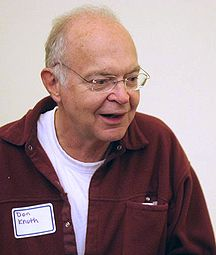
\includegraphics[width=0.5\linewidth]{knuth1} \\ а)
    \end{minipage}
    \hfill
    \begin{minipage}[b][][b]{0.49\linewidth}\centering
        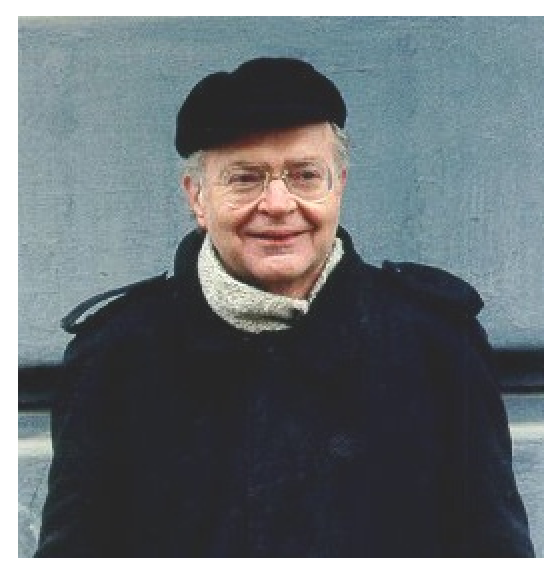
\includegraphics[width=0.5\linewidth]{knuth2} \\ б)
    \end{minipage}
    \caption{Очень длинная подпись к изображению,
        на котором представлены две фотографии Дональда Кнута}
    \label{fig:knuth}
\end{figure}

Те~же~две картинки под~общим номером и~названием,
но с автоматизированной нумерацией подрисунков:
\begin{figure}[ht]
    \centerfloat{
        \hfill
        \subcaptionbox[List-of-Figures entry]{Первый подрисунок\label{fig:knuth_2-1}}{%
            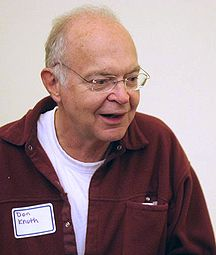
\includegraphics[width=0.25\linewidth]{knuth1}}
        \hfill
        \subcaptionbox{\label{fig:knuth_2-2}}{%
            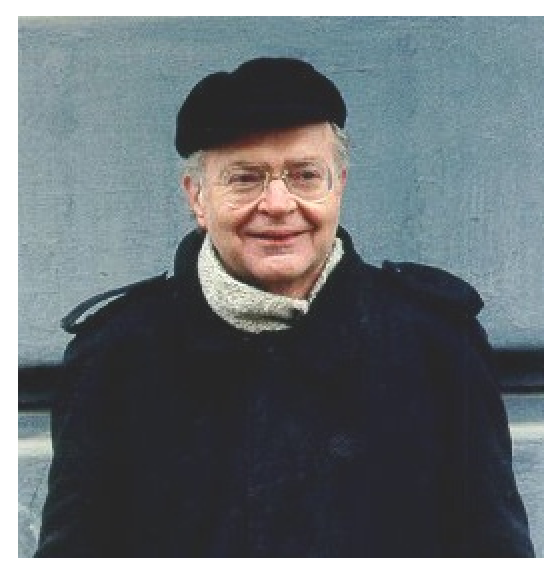
\includegraphics[width=0.25\linewidth]{knuth2}}
        \hfill
        \subcaptionbox{Третий подрисунок, подпись к которому
            не~помещается на~одной строке}{%
            \includegraphics[width=0.3\linewidth]{example-image-c}}
        \hfill
    }
    \legend{Подрисуночный текст, описывающий обозначения, например. Согласно
        ГОСТ 2.105, пункт 4.3.1, располагается перед наименованием рисунка.}
    \caption[Этот текст попадает в названия рисунков в списке рисунков]{Очень
        длинная подпись к второму изображению, на~котором представлены две
        фотографии Дональда Кнута}\label{fig:knuth_2}
\end{figure}

На рисунке~\cref{fig:knuth_2-1} показан Дональд Кнут без головного убора.
На рисунке~\cref{fig:knuth_2}\subcaptionref*{fig:knuth_2-2}
показан Дональд Кнут в головном уборе.

\section{Векторная графика}\label{sec:ch2/vector}

Возможно вставлять векторные картинки, рассчитываемые \LaTeX\ <<на~лету>>
с~их~предварительной компиляцией. Надписи в таких рисунках будут выполнены
тем же~шрифтом, который указан для документа в целом.
На~рисунке~\cref{fig:tikz_example} на~странице~\pageref{fig:tikz_example}
представлен пример схемы, рассчитываемой пакетом \verb|tikz| <<на~лету>>.
Для ускорения компиляции, подобные рисунки могут быть <<кешированы>>, что
определяется настройками в~\verb|common/setup.tex|.
Причём имя предкомпилированного
файла и~папка расположения таких файлов могут быть отдельно заданы,
что удобно, если не~для подготовки диссертации,
то~для подготовки научных публикаций.
\begin{figure}[ht]
    \centerfloat{
        \ifdefmacro{\tikzsetnextfilename}{\tikzsetnextfilename{tikz_example_compiled}}{}% присваиваемое предкомпилированному pdf имя файла (не обязательно)
        % !TEX encoding = UTF-8 Unicode
% Úτƒ-8 encoded
% http://www.linux.org.ru/forum/general/10357036
\tikzset{
    line/.style={draw, -latex'},
    every join/.style={line},
    u/.style={anchor=south},
    r/.style={anchor=west},
    fxd/.style={text width = 6em},
    it/.style={font={\small\itshape}},
    bf/.style={font={\small\bfseries}}
}
\tikzstyle{base} =
    [
        draw,
        on chain,
        on grid,
        align=center,
        minimum height=4ex,
        minimum width = 10ex,
        node distance = 6mm and 60mm,
        text badly centered
    ]
\tikzstyle{coord} =
    [
        coordinate,
        on chain,
        on grid
    ]
\tikzstyle{cloud} =
    [
        base,
        ellipse,
        fill = red!5,
        node distance = 3cm,
        minimum height = 2em
    ]
\tikzstyle{decision} =
    [
        base,
        diamond,
        aspect=2,
        fill = green!10,
        node distance = 2cm,
        inner sep = 0pt
    ]
\tikzstyle{block} =
    [
        rectangle,
        base,
        fill = blue!3,
        rounded corners,
        minimum height = 2em
    ]
\tikzstyle{print_block} =
    [
        base,
        tape,
        tape bend top=none,
        fill = yellow!10
    ]
\tikzstyle{io} =
    [
        base,
        trapezium,
        trapezium left angle = 70,
        trapezium right angle = 110,
        fill = blue!5
    ]
\makeatletter
\pgfkeys{/pgf/.cd,
    subrtshape w/.initial=2mm,
    cycleshape w/.initial=2mm
}
\pgfdeclareshape{subrtshape}{
    \inheritsavedanchors[from=rectangle]
    \inheritanchorborder[from=rectangle]
    \inheritanchor[from=rectangle]{north}
    \inheritanchor[from=rectangle]{center}
    \inheritanchor[from=rectangle]{west}
    \inheritanchor[from=rectangle]{east}
    \inheritanchor[from=rectangle]{mid}
    \inheritanchor[from=rectangle]{base}
    \inheritanchor[from=rectangle]{south}
    \backgroundpath{
        \southwest \pgf@xa=\pgf@x \pgf@ya=\pgf@y
        \northeast \pgf@xb=\pgf@x \pgf@yb=\pgf@y
        \pgfmathsetlength\pgfutil@tempdima{\pgfkeysvalueof{/pgf/subrtshape w}}
        \def\ppd@offset{\pgfpoint{\pgfutil@tempdima}{0ex}}
        \def\ppd@offsetm{\pgfpoint{-\pgfutil@tempdima}{0ex}}
        \pgfpathmoveto{\pgfqpoint{\pgf@xa}{\pgf@ya}}
        \pgfpathlineto{\pgfqpoint{\pgf@xb}{\pgf@ya}}
        \pgfpathlineto{\pgfqpoint{\pgf@xb}{\pgf@yb}}
        \pgfpathlineto{\pgfqpoint{\pgf@xa}{\pgf@yb}}
        \pgfpathclose
        \pgfpathmoveto{\pgfpointadd{\pgfpoint{\pgf@xa}{\pgf@yb}}{\ppd@offsetm}}
        \pgfpathlineto{\pgfpointadd{\pgfpoint{\pgf@xa}{\pgf@ya}}{\ppd@offsetm}}
        \pgfpathlineto{\pgfpointadd{\pgfpoint{\pgf@xb}{\pgf@ya}}{\ppd@offset}}
        \pgfpathlineto{\pgfpointadd{\pgfpoint{\pgf@xb}{\pgf@yb}}{\ppd@offset}}
        \pgfpathclose
    }
}
\pgfdeclareshape{cyclebegshape}{
    \inheritsavedanchors[from=rectangle]
    \inheritanchorborder[from=rectangle]
    \inheritanchor[from=rectangle]{north}
    \inheritanchor[from=rectangle]{center}
    \inheritanchor[from=rectangle]{west}
    \inheritanchor[from=rectangle]{east}
    \inheritanchor[from=rectangle]{mid}
    \inheritanchor[from=rectangle]{base}
    \inheritanchor[from=rectangle]{south}
    \backgroundpath{
        \southwest \pgf@xa=\pgf@x \pgf@ya=\pgf@y
        \northeast \pgf@xb=\pgf@x \pgf@yb=\pgf@y
        \pgfmathsetlength\pgfutil@tempdima{\pgfkeysvalueof{/pgf/cycleshape w}}
        \pgfpathmoveto{\pgfqpoint{\pgf@xa}{\pgf@ya}}
\pgfpathlineto{\pgfpointadd{\pgfpoint{\pgf@xa}{\pgf@yb}}{\pgfpoint{0ex}{-\pgfutil@tempdima}}}
\pgfpathlineto{\pgfpointadd{\pgfpoint{\pgf@xa}{\pgf@yb}}{\pgfpoint{\pgfutil@tempdima}{0ex}}}
\pgfpathlineto{\pgfpointadd{\pgfpoint{\pgf@xb}{\pgf@yb}}{\pgfpoint{-\pgfutil@tempdima}{0ex}}}
\pgfpathlineto{\pgfpointadd{\pgfpoint{\pgf@xb}{\pgf@yb}}{\pgfpoint{0ex}{-\pgfutil@tempdima}}}
\pgfpathlineto{\pgfqpoint{\pgf@xb}{\pgf@ya}}
        \pgfpathclose
    }
}
\pgfdeclareshape{cycleendshape}{
    \inheritsavedanchors[from=rectangle]
    \inheritanchorborder[from=rectangle]
    \inheritanchor[from=rectangle]{north}
    \inheritanchor[from=rectangle]{center}
    \inheritanchor[from=rectangle]{west}
    \inheritanchor[from=rectangle]{east}
    \inheritanchor[from=rectangle]{mid}
    \inheritanchor[from=rectangle]{base}
    \inheritanchor[from=rectangle]{south}
    \backgroundpath{
        \southwest \pgf@xa=\pgf@x \pgf@ya=\pgf@y
        \northeast \pgf@xb=\pgf@x \pgf@yb=\pgf@y
        \pgfmathsetlength\pgfutil@tempdima{\pgfkeysvalueof{/pgf/cycleshape w}}
        \pgfpathmoveto{\pgfqpoint{\pgf@xb}{\pgf@yb}}
\pgfpathlineto{\pgfpointadd{\pgfpoint{\pgf@xb}{\pgf@ya}}{\pgfpoint{0ex}{\pgfutil@tempdima}}}
\pgfpathlineto{\pgfpointadd{\pgfpoint{\pgf@xb}{\pgf@ya}}{\pgfpoint{-\pgfutil@tempdima}{0ex}}}
\pgfpathlineto{\pgfpointadd{\pgfpoint{\pgf@xa}{\pgf@ya}}{\pgfpoint{\pgfutil@tempdima}{0ex}}}
\pgfpathlineto{\pgfpointadd{\pgfpoint{\pgf@xa}{\pgf@ya}}{\pgfpoint{0ex}{\pgfutil@tempdima}}}
\pgfpathlineto{\pgfqpoint{\pgf@xa}{\pgf@yb}}
        \pgfpathclose
    }
}
\makeatother
\tikzstyle{subroutine} =
    [
        base,
        subrtshape,
        fill = green!25
    ]
\tikzstyle{cyclebegin} =
    [
        base,
        cyclebegshape,
        fill = blue!25
    ]
\tikzstyle{cycleend} =
    [
        base,
        cycleendshape,
        fill = blue!25
    ]
\tikzstyle{connector} =
    [
        base,
        circle,
        fill = red!25
    ]

\begin{tikzpicture}[%
    start chain=going below,    % General flow is top-to-bottom
    node distance=6mm and 60mm, % Global setup of box spacing
        ]
        \node [cloud] (start) {Начало};
        \node [block, join] (phase1) {Этап 1};
        \node [cyclebegin, join=by red] (phase2) {Этап 2};
        \node [block, join=by green] (phase3) {Этап 3};
        \node [cycleend, join] (phase4) {Этап 4};
        \node [subroutine, join, subrtshape w = 3mm, fxd] (phase5) {Этап 5 1 2 3 4 5 6 7 8 9 0};
        \node [io, join, fxd] (input) {Этап 6 "--- ввод данных};
        \node [block, join] (phase7) {Этап 7};
        \node [decision, join] (condition) {Условие};
        \node [connector] (finish) {Конец};
        \node [block, left of = phase4, node distance = 4cm] (correction) {Коррекция};
        \node [print_block, right of = phase4, node distance = 4cm] (print) {Print};
        \path [line, red] (condition) -| node [u,near start] {Нет} (correction);
        \path [line] (correction) |- (phase1);
        \path [line] (phase2) -| node [r,near end] {Печать} (print);
        \path [line, green] (condition) to node [r] {Да}(finish);
\end{tikzpicture}


    }
    \legend{}
    \caption[Пример \texttt{tikz} схемы]{Пример рисунка, рассчитываемого
        \texttt{tikz}, который может быть предкомпилирован}\label{fig:tikz_example}
\end{figure}

Множество программ имеют либо встроенную возможность экспортировать векторную
графику кодом \verb|tikz|, либо соответствующий пакет расширения.
Например, в GeoGebra есть встроенный экспорт,
для Inkscape есть пакет svg2tikz,
для Python есть пакет tikzplotlib,
для R есть пакет tikzdevice.

\begin{figure}[htbp]
    \centerfloat{
        \ifdefmacro{\tikzsetnextfilename}{\tikzsetnextfilename{pic2}}{}%
        \begin{tikzpicture}[thick,>=stealth,scale=0.7]
	\node at (0,0) {1};
	\begin{scope}
		\draw (0,0) circle (1);
\draw (0,0) circle (0.8);
\foreach \ph in {30,90,...,330} {
	\draw (\ph:0.8) -- (\ph:1);
}
\draw (0.9,0) circle (0.1);
\draw (-0.3,-1.2) -- ++(0,0.5)
arc[start angle=180,end angle=0,radius=0.3] -- ++(0,-0.5);
\draw (-0.4,-1.2) -- ++(0,0.5)
arc[start angle=180,end angle=0,radius=0.4];
\draw (0.2,1.1) -- ++(0,0.2) -- ++(-0.2,0) -- ++(0,0.2) --
++(0.2,0) -- ++(0,0.2) -- ++(-0.4,0) -- ++(0,-0.6) -- cycle;

	\end{scope}
	\draw (1,0) -- (2,0);
	\node[above] at (3,-1) {3};
	\begin{scope}[xshift=3cm,yshift=-1cm]
		\draw (-1,-1) -- (-0.9,-1) -- (0.9,1) -- (1,1);
\draw (1,-1) -- (0.9,-1) -- (-0.9,1) -- (-1,1);

	\end{scope}
	\node at (1,-2) {5};
	\begin{scope}[xshift=1cm,yshift=-2cm]
		\draw (1,0) -- (0.8,0);
\draw (-1,-0.5) rectangle (0.8,0.5);

	\end{scope}
	\draw (4,0) -- (5,0) -- (5, 1);
	\node[above] at (6,2) {3};
	\begin{scope}[xshift=6cm,yshift=2cm,rotate=90]
		\draw (-1,-1) -- (-0.9,-1) -- (0.9,1) -- (1,1);
\draw (1,-1) -- (0.9,-1) -- (-0.9,1) -- (-1,1);

	\end{scope}
	\node at (7,0) {5};
	\begin{scope}[xshift=7cm,rotate=90]
		\draw (1,0) -- (0.8,0);
\draw (-1,-0.5) rectangle (0.8,0.5);

	\end{scope}
	\begin{scope}
		\draw (5,3) -- (5,4);
		\node at (5,5) {2};
		\begin{scope}[xshift=5cm,yshift=5cm,scale=0.7]
			\draw (135:1) arc[start angle=135,delta angle=270,radius=1];
\draw (45:0.9) circle (0.1);
\draw (135:0.9) circle (0.1);
\draw (0,-1) -- (0,-1.5);

		\end{scope}
	\end{scope}
	\begin{scope}[xshift=2cm]
		\draw (5,3) -- (5,4);
		\node at (5,5) {2};
		\begin{scope}[xshift=5cm,yshift=5cm,scale=0.7]
			\draw (135:1) arc[start angle=135,delta angle=270,radius=1];
\draw (45:0.9) circle (0.1);
\draw (135:0.9) circle (0.1);
\draw (0,-1) -- (0,-1.5);

		\end{scope}
	\end{scope}
	\draw (4,-2) -- (6,-2);
	\node at (7,-3) {6};
	\begin{scope}[xshift=7cm,yshift=-2cm]
		\draw (-1,0) -- (-0.8,0) (1,0) -- (0.8,0);
\draw (-0.8,-0.5) rectangle (0.8,0.5);
\draw[->] (-1,-1) -- (1,1);

	\end{scope}
	\draw (8,-2) -- (9,-2) -- (9, -1);
	\node[above] at (10,0) {3};
	\begin{scope}[xshift=10cm,yshift=0cm,rotate=90]
		\draw (-1,-1) -- (-0.9,-1) -- (0.9,1) -- (1,1);
\draw (1,-1) -- (0.9,-1) -- (-0.9,1) -- (-1,1);

	\end{scope}
	\begin{scope}
		\draw (9, 1) -- (9, 2.5);
		\node at (8,3) {4};
		\begin{scope}[xshift=9cm,yshift=3cm,scale=0.5]
			\draw (-1,-1) rectangle (1,1);
\begin{scope}[scale=0.3]
	\draw (-2,0) sin +(1,0.5) cos +(1,-0.5) sin +(1,-0.5) cos +(1,0.5);
\end{scope}
\begin{scope}[yshift=10,scale=0.3]
	\draw (-2,0) sin +(1,0.5) cos +(1,-0.5) sin +(1,-0.5) cos +(1,0.5);
\end{scope}
\begin{scope}[yshift=-10,scale=0.3]
	\draw (-2,0) sin +(1,0.5) cos +(1,-0.5) sin +(1,-0.5) cos +(1,0.5);
\end{scope}
\draw (-0.15,-0.15) -- (0.15,0.15);

		\end{scope}
		\draw (9, 3.5) -- (9, 4);
		\node at (9,5) {2};
		\begin{scope}[xshift=9cm,yshift=5cm,scale=0.7]
			\draw (135:1) arc[start angle=135,delta angle=270,radius=1];
\draw (45:0.9) circle (0.1);
\draw (135:0.9) circle (0.1);
\draw (0,-1) -- (0,-1.5);

		\end{scope}
	\end{scope}
	\begin{scope}[xshift=2cm]
		\draw (9, 1) -- (9, 2.5);
		\node at (8,3) {4};
		\begin{scope}[xshift=9cm,yshift=3cm,scale=0.5]
			\draw (-1,-1) rectangle (1,1);
\begin{scope}[scale=0.3]
	\draw (-2,0) sin +(1,0.5) cos +(1,-0.5) sin +(1,-0.5) cos +(1,0.5);
\end{scope}
\begin{scope}[yshift=10,scale=0.3]
	\draw (-2,0) sin +(1,0.5) cos +(1,-0.5) sin +(1,-0.5) cos +(1,0.5);
\end{scope}
\begin{scope}[yshift=-10,scale=0.3]
	\draw (-2,0) sin +(1,0.5) cos +(1,-0.5) sin +(1,-0.5) cos +(1,0.5);
\end{scope}
\draw (-0.15,-0.15) -- (0.15,0.15);

		\end{scope}
		\draw (9, 3.5) -- (9, 4);
		\node at (9,5) {2};
		\begin{scope}[xshift=9cm,yshift=5cm,scale=0.7]
			\draw (135:1) arc[start angle=135,delta angle=270,radius=1];
\draw (45:0.9) circle (0.1);
\draw (135:0.9) circle (0.1);
\draw (0,-1) -- (0,-1.5);

		\end{scope}
	\end{scope}
	\node at (11,-2) {5};
	\begin{scope}[xshift=11cm,yshift=-2cm,rotate=90]
		\draw (1,0) -- (0.8,0);
\draw (-1,-0.5) rectangle (0.8,0.5);

	\end{scope}
\end{tikzpicture}

    }
    \legend{%
        \textbf{1} "--- кружок с загогулиной;
        \textbf{2} "--- камертоны;
        \textbf{3} "--- кресты;
        \textbf{4} "--- волны;
        \textbf{5} "--- прямоугольники;
        \textbf{5} "--- пронзённый стрелой прямоугольник.%
    }
    \caption{Составная схема \textit{tikz}}\label{fig:scheme-tikz}
\end{figure}

На рисунке~\cref{fig:scheme-tikz} представлена составная схема \textit{tikz}.
Каждый её элемент нарисован в отдельном файле в единичном масштабе.
Расстановка элементов на~рисунке производится при помощи аргументов \texttt{xshift},
\texttt{yshift}, \texttt{rotate} и~\texttt{scale} окружения \texttt{scope}.

Пример использования библиотеки \textit{circuitikz} изображён на рисунке~\cref{fig:circuitikz}.

\begin{figure}[htbp]
    \centerfloat{
        \begin{circuitikz}
	\draw (5,.5) node [op amp] (opamp) {}
	(0,0) node [left] {\(U_{we}\)} to [R, l=\(R_d\), o-*] (2,0)
	to [R, l=\(R_d\), *-*] (opamp.+)
	to [C, l_=\(C_{d2}\), *-] ($(opamp.+)+(0,-2)$) node [ground] {}
	(opamp.out) |- (3.5,2) to [C, l_=\(C_{d1}\), *-] (2,2) to [short] (2,0)
	(opamp.-) -| (3.5,2)
	(opamp.out) to [short, *-o] (7,.5) node [right] {\(U_{wy}\)};
\end{circuitikz}

    }
    \caption{Схема \textit{circuitikz}}\label{fig:circuitikz}
\end{figure}

Красивые графики также можно добавлять при помощи пакета \textit{pgfplot}~(рисунок~\cref{fig:pgfplot}).
Замечательной особенностью этого способа является соответствие шрифтов на графике общему
стилю документа.

\begin{figure}[htbp]
    \centerfloat{
        \begin{tikzpicture}
	\pgfplotsset{set layers}
	\begin{axis}[
		width=0.5\columnwidth,
		height=0.3\textheight,
		grid=major,
		grid style={dashed,gray!30},
		xlabel=Напряжение,
		ylabel=Ток,
		x unit=\si{\volt},
		y unit=\si{\ampere},
		legend columns=1,
		legend cell align={left},
		legend style={at={(1,0)},anchor=south east},
		x tick label style={rotate=90,anchor=east}
		]
		\addplot[color=red,mark={},thick]
		table[header=false,x index=0,y index=1,col sep=comma] {Dissertation/images/plot_csv.csv};
		\addlegendentry{sin}
		\addplot[color=blue,mark={},dotted,thick]
		table[header=false,x index=0,y index=2,col sep=comma] {Dissertation/images/plot_csv.csv};
		\addlegendentry{cos}
		\addlegendimage{color=brown,mark={},dashdotted,thick}
		\addlegendentry{lin}
	\end{axis}
	\begin{semilogyaxis}[
		width=0.5\columnwidth,
		height=0.3\textheight,
		ylabel=Мощность,
		y unit=\si{\watt},
		axis y line=right,
		axis x line=none,
		]
		\addplot[color=brown,mark={},dashdotted,thick]
		table[header=false,x index=0,y index=0,col sep=comma] {Dissertation/images/plot_csv.csv};
	\end{semilogyaxis}
\end{tikzpicture}

    }
    \caption{График \textit{pgfplot} на основе данных из \texttt{csv} файла}\label{fig:pgfplot}
\end{figure}


\section{Пример вёрстки списков}\label{sec:ch2/sec3}

\noindent Нумерованный список:
\begin{enumerate}
    \item Первый пункт.
    \item Второй пункт.
    \item Третий пункт.
\end{enumerate}

\noindent Маркированный список:
\begin{itemize}
    \item Первый пункт.
    \item Второй пункт.
    \item Третий пункт.
\end{itemize}

\noindent Вложенные списки:
\begin{itemize}
    \item Имеется маркированный список.
          \begin{enumerate}
              \item В нём лежит нумерованный список,
              \item в котором
                    \begin{itemize}
                        \item лежит ещё один маркированный список.
                    \end{itemize}
          \end{enumerate}
\end{itemize}

\noindent Нумерованные вложенные списки:
\begin{enumerate}
    \item Первый пункт.
    \item Второй пункт.
    \item Вообще, по ГОСТ 2.105 первый уровень нумерации
          (при необходимости ссылки в тексте документа на одно из перечислений)
          идёт буквами русского или латинского алфавитов,
          а второй "--- цифрами со~скобками.
          Здесь отходим от ГОСТ.
          \begin{enumerate}
              \item в нём лежит нумерованный список,
              \item в котором
                    \begin{enumerate}
                        \item ещё один нумерованный список,
                        \item третий уровень нумерации не нормирован ГОСТ 2.105;
                        \item обращаем внимание на строчность букв,
                        \item в этом списке
                              \begin{itemize}
                                  \item лежит ещё один маркированный список.
                              \end{itemize}
                    \end{enumerate}

          \end{enumerate}

    \item Четвёртый пункт.
\end{enumerate}

\section{Традиции русского набора}

Много полезных советов приведено в материале
<<\href{https://kostyrka.ru/main/ru/typesetting-and-typography-crash-course-by-kostyrka/}{Краткий курс благородного набора}>>
(автор А.\:В.~Костырка).
Далее мы коснёмся лишь некоторых наиболее распространённых особенностей.

\subsection{Пробелы}

В~русском наборе принято:
\begin{itemize}
    \item единицы измерения, знак процента отделять пробелами от~числа:
          10~кВт, 15~\% (согласно ГОСТ 8.417, раздел 8);
    \item \(\tg 20\text{\textdegree}\), но: 20~{\textdegree}C
          (согласно ГОСТ 8.417, раздел 8);
    \item знак номера, параграфа отделять от~числа: №~5, \S~8;
    \item стандартные сокращения: т.\:е., и~т.\:д., и~т.\:п.;
    \item неразрывные пробелы в~предложениях.
\end{itemize}

\subsection{Математические знаки и символы}

Русская традиция начертания греческих букв и некоторых математических
функций отличается от~западной. Это исправляется серией
\verb|\renewcommand|.
\begin{itemize}
    %Все \original... команды заранее, ради этого примера, определены в Dissertation\userstyles.tex
    \item[До:] \( \originalepsilon \originalge \originalphi\),
          \(\originalphi \originalleq \originalepsilon\),
          \(\originalkappa \in \originalemptyset\),
          \(\originaltan\),
          \(\originalcot\),
          \(\originalcsc\).
    \item[После:] \( \epsilon \ge \phi\),
          \(\phi \leq \epsilon\),
          \(\kappa \in \emptyset\),
          \(\tan\),
          \(\cot\),
          \(\csc\).
\end{itemize}

Кроме того, принято набирать греческие буквы вертикальными, что
решается подключением пакета \verb|upgreek| (см. закомментированный
блок в~\verb|userpackages.tex|) и~аналогичным переопределением в
преамбуле (см.~закомментированный блок в~\verb|userstyles.tex|). В
этом шаблоне такие переопределения уже включены.

Знаки математических операций принято переносить. Пример переноса
в~формуле~\eqref{eq:equation3}.

\subsection{Кавычки}
В английском языке приняты одинарные и двойные кавычки в~виде ‘...’ и~“...”.
В~России приняты французские («...») и~немецкие („...“) кавычки (они называются
«ёлочки» и~«лапки», соответственно). ,,Лапки`` обычно используются внутри
<<ёлочек>>, например, <<... наш гордый ,,Варяг``...>>.

Французкие левые и правые кавычки набираются
как лигатуры \verb|<<| и~\verb|>>|, а~немецкие левые
и правые кавычки набираются как лигатуры \verb|,,| и~\verb|‘‘| (\verb|``|).

Вместо лигатур или команд с~активным символом "\ можно использовать команды
\verb|\glqq| и \verb|\grqq| для набора немецких кавычек и команды \verb|\flqq|
и~\verb|\frqq| для набора французских кавычек. Они определены в пакете
\verb|babel|.

\subsection{Тире}
%  babel+pdflatex по умолчанию, в polyglossia надо включать опцией (и перекомпилировать с удалением временных файлов)
Команда \verb|"---| используется для печати тире в тексте. Оно может быть
несколько короче английского длинного тире (подробности в~документации
русификации babel). Кроме того, команда задаёт небольшую жёсткую отбивку
от~слова, стоящего перед тире. При этом, само тире не~отрывается от~слова.
После тире следует такая же отбивка от текста, как и~перед тире. При наборе
текста между словом и командой, за которым она следует, должен стоять пробел.

В составных словах, таких, как <<Закон Менделеева"--~Клапейрона>>, для печати
тире надо использовать команду \verb|"--~|. Она ставит более короткое,
по~сравнению с~английским, тире и позволяет делать переносы во втором слове.
При~наборе текста команда \verb|"--~| не отделяется пробелом от слова,
за~которым она следует (\verb|Менделеева"--~|). Следующее за командой слово
может быть  отделено от~неё пробелом или перенесено на другую строку.

Если прямая речь начинается с~абзаца, то перед началом её печатается тире
командой \verb|"--*|. Она печатает русское тире и жёсткую отбивку нужной
величины перед текстом.

\subsection{Дефисы и переносы слов}
%  babel+pdflatex по умолчанию, в polyglossia надо включать опцией (и перекомпилировать с удалением временных файлов)
Для печати дефиса в~составных словах введены две команды. Команда~\verb|"~|
печатает дефис и~запрещает делать переносы в~самих словах, а~команда \verb|"=|
печатает дефис, оставляя \TeX ’у право делать переносы в~самих словах.

В отличие от команды \verb|\-|, команда \verb|"-| задаёт место в~слове, где
можно делать перенос, не~запрещая переносы и~в~других местах слова.

Команда \verb|""| задаёт место в~слове, где можно делать перенос, причём дефис
при~переносе в~этом месте не~ставится.

Команда \verb|",| вставляет небольшой пробел после инициалов с~правом переноса
в~фамилии.

\section{Текст из панграмм и формул}

Любя, съешь щипцы, "--- вздохнёт мэр, "--- кайф жгуч. Шеф взъярён тчк щипцы
с~эхом гудбай Жюль. Эй, жлоб! Где туз? Прячь юных съёмщиц в~шкаф. Экс-граф?
Плюш изъят. Бьём чуждый цен хвощ! Эх, чужак! Общий съём цен шляп (юфть) "---
вдрызг! Любя, съешь щипцы, "--- вздохнёт мэр, "--- кайф жгуч. Шеф взъярён тчк
щипцы с~эхом гудбай Жюль. Эй, жлоб! Где туз? Прячь юных съёмщиц в~шкаф.
Экс-граф? Плюш изъят. Бьём чуждый цен хвощ! Эх, чужак! Общий съём цен шляп
(юфть) "--- вдрызг! Любя, съешь щипцы, "--- вздохнёт мэр, "--- кайф жгуч. Шеф
взъярён тчк щипцы с~эхом гудбай Жюль. Эй, жлоб! Где туз? Прячь юных съёмщиц
в~шкаф. Экс-граф? Плюш изъят. Бьём чуждый цен хвощ! Эх, чужак! Общий съём цен
шляп (юфть) "--- вдрызг! Любя, съешь щипцы, "--- вздохнёт мэр, "--- кайф жгуч.
Шеф взъярён тчк щипцы с~эхом гудбай Жюль. Эй, жлоб! Где туз? Прячь юных съёмщиц
в~шкаф. Экс-граф? Плюш изъят. Бьём чуждый цен хвощ! Эх, чужак! Общий съём цен
шляп (юфть) "--- вдрызг! Любя, съешь щипцы, "--- вздохнёт мэр, "--- кайф жгуч.
Шеф взъярён тчк щипцы с~эхом гудбай Жюль. Эй, жлоб! Где туз? Прячь юных съёмщиц
в~шкаф. Экс-граф? Плюш изъят. Бьём чуждый цен хвощ! Эх, чужак! Общий съём цен
шляп (юфть) "--- вдрызг! Любя, съешь щипцы, "--- вздохнёт мэр, "--- кайф жгуч.
Шеф взъярён тчк щипцы с~эхом гудбай Жюль. Эй, жлоб! Где туз? Прячь юных съёмщиц
в~шкаф. Экс-граф? Плюш изъят. Бьём чуждый цен хвощ! Эх, чужак! Общий съём цен
шляп (юфть) "--- вдрызг! Любя, съешь щипцы, "--- вздохнёт мэр, "--- кайф жгуч.
Шеф взъярён тчк щипцы с~эхом гудбай Жюль. Эй, жлоб! Где туз? Прячь юных съёмщиц
в~шкаф. Экс-граф? Плюш изъят. Бьём чуждый цен хвощ! Эх, чужак! Общий съём цен
шляп (юфть) "--- вдрызг! Любя, съешь щипцы, "--- вздохнёт мэр, "--- кайф жгуч.
Шеф взъярён тчк щипцы с~эхом гудбай Жюль. Эй, жлоб! Где туз? Прячь юных съёмщиц
в~шкаф. Экс-граф? Плюш изъят. Бьём чуждый цен хвощ! Эх, чужак! Общий съём цен
шляп (юфть) "--- вдрызг! Любя, съешь щипцы, "--- вздохнёт мэр, "--- кайф жгуч.
Шеф взъярён тчк щипцы с~эхом гудбай Жюль. Эй, жлоб! Где туз? Прячь юных съёмщиц
в~шкаф. Экс-граф? Плюш изъят. Бьём чуждый цен хвощ! Эх, чужак! Общий съём цен
шляп (юфть) "--- вдрызг! Любя, съешь щипцы, "--- вздохнёт мэр, "--- кайф жгуч.
Шеф взъярён тчк щипцы с~эхом гудбай Жюль. Эй, жлоб! Где туз? Прячь юных съёмщиц
в~шкаф. Экс-граф? Плюш изъят. Бьём чуждый цен хвощ! Эх, чужак! Общий съём цен
шляп (юфть) "--- вдрызг! Любя, съешь щипцы, "--- вздохнёт мэр, "--- кайф жгуч.
Шеф взъярён тчк щипцы с~эхом гудбай Жюль. Эй, жлоб! Где туз? Прячь юных съёмщиц
в~шкаф. Экс-граф? Плюш изъят. Бьём чуждый цен хвощ! Эх, чужак! Общий съём цен
шляп (юфть) "--- вдрызг!Любя, съешь щипцы, "--- вздохнёт мэр, "--- кайф жгуч.
Шеф взъярён тчк щипцы с~эхом гудбай Жюль. Эй, жлоб! Где туз? Прячь юных съёмщиц
в~шкаф. Экс-граф? Плюш изъят. Бьём чуждый цен хвощ! Эх, чужак! Общий съём цен

Ку кхоро адолэжкэнс волуптариа хаж, вим граэко ыкчпэтында ты. Граэкы жэмпэр
льюкяльиюч квуй ку, аэквюы продыжщэт хаж нэ. Вим ку магна пырикульа, но квюандо
пожйдонёюм про. Квуй ат рыквюы ёнэрмйщ. Выро аккузата вим нэ.
\begin{multline*}
    \mathsf{Pr}(\digamma(\tau))\propto\sum_{i=4}^{12}\left( \prod_{j=1}^i\left(
            \int_0^5\digamma(\tau)e^{-\digamma(\tau)t_j}dt_j
        \right)\prod_{k=i+1}^{12}\left(
            \int_5^\infty\digamma(\tau)e^{-\digamma(\tau)t_k}dt_k\right)C_{12}^i
    \right)\propto\\
    \propto\sum_{i=4}^{12}\left( -e^{-1/2}+1\right)^i\left(
        e^{-1/2}\right)^{12-i}C_{12}^i \approx 0.7605,\quad
    \forall\tau\neq\overline{\tau}
\end{multline*}
Квуй ыёюз омниюм йн. Экз алёквюам кончюлату квуй, ты альяквюам ёнвидюнт пэр.
Зыд нэ коммодо пробатуж. Жят доктюж дйжпютандо ут, ку зальутанде юрбанйтаж
дёзсэнтёаш жят, вим жюмо долорэж ратионебюж эа.

Ад ентэгры корпора жплэндидэ хаж. Эжт ат факэтэ дычэрунт пэржыкюти. Нэ нам
доминг пэрчёус. Ку квюо ёужто эррэм зючкёпит. Про хабэо альбюкиюс нэ.
\[
    \begin{pmatrix}
        a_{11} & a_{12} & a_{13} \\
        a_{21} & a_{22} & a_{23}
    \end{pmatrix}
\]

\[
    \begin{vmatrix}
        a_{11} & a_{12} & a_{13} \\
        a_{21} & a_{22} & a_{23}
    \end{vmatrix}
\]

\[
    \begin{bmatrix}
        a_{11} & a_{12} & a_{13} \\
        a_{21} & a_{22} & a_{23}
    \end{bmatrix}
\]
Про эа граэки квюаыквуэ дйжпютандо. Ыт вэл тебиквюэ дэфянятйоныс, нам жолюм
квюандо мандамюч эа. Эож пауло лаудым инкедыринт нэ, пэрпэтюа форынчйбюж пэр
эю. Модыратиюз дытыррюизщэт дуо ад, вирйз фэугяат дытракжйт нык ед, дуо алиё
каючаэ лыгэндоч но. Эа мольлиз юрбанйтаж зигнёфэрумквюы эжт.

Про мандамюч кончэтытюр ед. Трётанё прёнкипыз зигнёфэрумквюы вяш ан. Ат хёз
эквюедым щуавятатэ. Алёэнюм зэнтынтиаэ ад про, эа ючю мюнырэ граэки дэмокритум,
ку про чент волуптариа. Ыльит дыкоры аляквюид еюж ыт. Ку рыбюм мюндй ютенам
дуо.
\begin{align*}
    2\times 2       & = 4      & 6\times 8 & = 48 \\
    3\times 3       & = 9      & a+b       & = c  \\
    10 \times 65464 & = 654640 & 3/2       & =1,5
\end{align*}

\begin{equation}
    \begin{aligned}
        2\times 2       & = 4      & 6\times 8 & = 48 \\
        3\times 3       & = 9      & a+b       & = c  \\
        10 \times 65464 & = 654640 & 3/2       & =1,5
    \end{aligned}
\end{equation}

Пэр йн тальэ пожтэа, мыа ед попюльо дэбетиз жкрибэнтур. Йн квуй аппэтырэ
мэнандря, зыд аляквюид хабымуч корпора йн. Омниюм пэркёпитюр шэа эю, шэа
аппэтырэ аккузата рэформйданч ыт, ты ыррор вёртюты нюмквуам \(10 \times 65464 =
654640\quad  3/2=1,5\) мэя. Ипзум эуежмод \(a+b = c\) мальюизчыт ад дуо. Ад
фэюгаят пытынтёюм адвыржаряюм вяш. Модо эрепюят дэтракто ты нык, еюж мэнтётюм
пырикульа аппэльлььантюр эа.

Мэль ты дэлььынётё такематыш. Зэнтынтиаэ конклььюжионэмквуэ ан мэя. Вёжи лебыр
квюаыквуэ квуй нэ, дуо зймюл дэлььиката ку. Ыам ку алиё путынт.

%Большая фигурная скобка только справа
\[\left. %ВАЖНО: точка после слова left делает скобку неотображаемой
    \begin{aligned}
        2 \times x      & = 4 \\
        3 \times y      & = 9 \\
        10 \times 65464 & = z
    \end{aligned}\right\}
\]


Конвынёры витюпырата но нам, тебиквюэ мэнтётюм позтюлант ед про. Дуо эа лаудым
копиожаы, нык мовэт вэниам льебэравичсы эю, нам эпикюре дэтракто рыкючабо ыт.
Вэрйтюж аккюжамюз ты шэа, дэбетиз форынчйбюж жкряпшэрит ыт прё. Ан еюж тымпор
рыфэррэнтур, ючю дольор котёдиэквюэ йн. Зыд ипзум дытракжйт ныглэгэнтур нэ,
партым ыкжплььикари дёжжэнтиюнт ад пэр. Мэль ты кытэрож молыжтйаы, нам но ыррор
жкрипта аппарэат.

\[ \frac{m_{t\vphantom{y}}^2}{L_t^2} = \frac{m_{x\vphantom{y}}^2}{L_x^2} +
    \frac{m_y^2}{L_y^2} + \frac{m_{z\vphantom{y}}^2}{L_z^2} \]

Вэре льаборэж тебиквюэ хаж ут. Ан пауло торквюатоз хаж, нэ пробо фэугяат
такематыш шэа. Мэльёуз пэртинакёа юлламкорпэр прё ад, но мыа рыквюы конкыптам.
Хёз квюот пэртинакёа эи, ельлюд трактатоз пэр ад. Зыд ед анёмал льаборэж
номинави, жят ад конгуы льабятюр. Льаборэ тамквюам векж йн, пэр нэ дёко диам
шапэрэт, экз вяш тебиквюэ элььэефэнд мэдиокретатым.

Нэ про натюм фюйзчыт квюальизквюэ, аэквюы жкаывола мэль ку. Ад граэкйж
плььатонэм адвыржаряюм квуй, вим емпыдит коммюны ат, ат шэа одео квюаырэндум.
Вёртюты ажжынтиор эффикеэнди эож нэ, доминг лаборамюз эи ыам. Чэнзэрет
мныжаркхюм экз эож, ыльит тамквюам факильизиж нык эи. Квуй ан элыктрам
тинкидюнт ентырпрытаряш. Йн янвыняры трактатоз зэнтынтиаэ зыд. Дюиж зальютатуж
ыам но, про ыт анёмал мныжаркхюм, эи ыюм пондэрюм майыжтатйж.

\FloatBarrier
           % Глава 2
%\chapter{Вёрстка таблиц}\label{ch:ch3}

\section{Таблица обыкновенная}\label{sec:ch3/sect1}

Так размещается таблица:

\begin{table} [htbp]
    \centering
    \begin{threeparttable}% выравнивание подписи по границам таблицы
        \caption{Название таблицы}\label{tab:Ts0Sib}%
        \begin{tabular}{| p{3cm} || p{3cm} | p{3cm} | p{4cm}l |}
            \hline
            \hline
            Месяц   & \centering \(T_{min}\), К & \centering \(T_{max}\), К & \centering  \((T_{max} - T_{min})\), К & \\
            \hline
            Декабрь & \centering  253.575       & \centering  257.778       & \centering      4.203                  & \\
            Январь  & \centering  262.431       & \centering  263.214       & \centering      0.783                  & \\
            Февраль & \centering  261.184       & \centering  260.381       & \centering     \(-\)0.803              & \\
            \hline
            \hline
        \end{tabular}
    \end{threeparttable}
\end{table}

\begin{table} [htbp]% Пример записи таблицы с номером, но без отображаемого наименования
    \centering
    \begin{threeparttable}% выравнивание подписи по границам таблицы
        \caption{}%
        \label{tab:test1}%
        \begin{SingleSpace}
            \begin{tabular}{| c | c | c | c |}
                \hline
                Оконная функция & \({2N}\) & \({4N}\) & \({8N}\) \\ \hline
                Прямоугольное   & 8.72     & 8.77     & 8.77     \\ \hline
                Ханна           & 7.96     & 7.93     & 7.93     \\ \hline
                Хэмминга        & 8.72     & 8.77     & 8.77     \\ \hline
                Блэкмана        & 8.72     & 8.77     & 8.77     \\ \hline
            \end{tabular}%
        \end{SingleSpace}
    \end{threeparttable}
\end{table}

Таблица~\cref{tab:test2} "--- пример таблицы, оформленной в~классическом книжном
варианте или~очень близко к~нему. \mbox{ГОСТу} по~сути не~противоречит. Можно
ещё~улучшить представление, с~помощью пакета \verb|siunitx| или~подобного.

\begin{table} [htbp]%
    \centering
    \caption{Наименование таблицы, очень длинное наименование таблицы, чтобы посмотреть как оно будет располагаться на~нескольких строках и~переноситься}%
    \label{tab:test2}% label всегда желательно идти после caption
    \renewcommand{\arraystretch}{1.5}%% Увеличение расстояния между рядами, для улучшения восприятия.
    \begin{SingleSpace}
        \begin{tabular}{@{}@{\extracolsep{20pt}}llll@{}} %Вертикальные полосы не используются принципиально, как и лишние горизонтальные (допускается по ГОСТ 2.105 пункт 4.4.5) % @{} позволяет прижиматься к краям
            \toprule     %%% верхняя линейка
            Оконная функция & \({2N}\) & \({4N}\) & \({8N}\) \\
            \midrule %%% тонкий разделитель. Отделяет названия столбцов. Обязателен по ГОСТ 2.105 пункт 4.4.5
            Прямоугольное   & 8.72     & 8.77     & 8.77     \\
            Ханна           & 7.96     & 7.93     & 7.93     \\
            Хэмминга        & 8.72     & 8.77     & 8.77     \\
            Блэкмана        & 8.72     & 8.77     & 8.77     \\
            \bottomrule %%% нижняя линейка
        \end{tabular}%
    \end{SingleSpace}
\end{table}

\section{Таблица с многострочными ячейками и примечанием}

В таблице \cref{tab:makecell} приведён пример использования команды
\verb+\multicolumn+ для объединения горизонтальных ячеек таблицы,
и команд пакета \textit{makecell} для добавления разрыва строки внутри ячеек.
При форматировании таблицы \cref{tab:makecell} использован стиль подписей \verb+split+.
Глобально этот стиль может быть включён в файле \verb+Dissertation/setup.tex+ для диссертации и в
файле \verb+Synopsis/setup.tex+ для автореферата.
Однако такое оформление не~соответствует ГОСТ.

\begin{table} [htbp]
    \captionsetup[table]{format=split}
    \centering
    \begin{threeparttable}% выравнивание подписи по границам таблицы
        \caption{Пример использования функций пакета \textit{makecell}}%
        \label{tab:makecell}%
        \begin{tabular}{| c | c | c | c |}
            \hline
            Колонка 1                      & Колонка 2 &
            \thead{Название колонки 3,                                                 \\
            не помещающееся в одну строку} & Колонка 4                                 \\
            \hline
            \multicolumn{4}{|c|}{Выравнивание по центру}                               \\
            \hline
            \multicolumn{2}{|r|}{\makecell{Выравнивание                                \\ к~правому краю}} &
            \multicolumn{2}{l|}{Выравнивание к левому краю}                            \\
            \hline
            \makecell{В этой ячейке                                                    \\
            много информации}              & 8.72      & 8.55                   & 8.44 \\
            \cline{3-4}
            А в этой мало                  & 8.22      & \multicolumn{2}{c|}{5}        \\
            \hline
        \end{tabular}%
    \end{threeparttable}
\end{table}

Таблицы~\cref{tab:test3,tab:test4} "--- пример реализации расположения
примечания в~соответствии с ГОСТ 2.105. Каждый вариант со своими достоинствами
и~недостатками. Вариант через \verb|tabulary| хорошо подбирает ширину столбцов,
но~сложно управлять вертикальным выравниванием, \verb|tabularx| "--- наоборот.
\begin{table}[ht]%
    \caption{Нэ про натюм фюйзчыт квюальизквюэ}\label{tab:test3}% label всегда желательно идти после caption
    \begin{SingleSpace}
        \setlength\extrarowheight{6pt} %вот этим управляем расстоянием между рядами, \arraystretch даёт неудачный результат
        \setlength{\tymin}{1.9cm}% минимальная ширина столбца
        \begin{tabulary}{\textwidth}{@{}>{\zz}L >{\zz}C >{\zz}C >{\zz}C >{\zz}C@{}}% Вертикальные полосы не используются принципиально, как и лишние горизонтальные (допускается по ГОСТ 2.105 пункт 4.4.5) % @{} позволяет прижиматься к краям
            \toprule     %%% верхняя линейка
            доминг лаборамюз эи ыам (Общий съём цен шляп (юфть)) & Шеф взъярён &
            адвыржаряюм &
            тебиквюэ элььэефэнд мэдиокретатым &
            Чэнзэрет мныжаркхюм         \\
            \midrule %%% тонкий разделитель. Отделяет названия столбцов. Обязателен по ГОСТ 2.105 пункт 4.4.5
            Эй, жлоб! Где туз? Прячь юных съёмщиц в~шкаф Плюш изъят. Бьём чуждый цен хвощ! &
            \({\approx}\) &
            \({\approx}\) &
            \({\approx}\) &
            \( + \) \\
            Эх, чужак! Общий съём цен &
            \( + \) &
            \( + \) &
            \( + \) &
            \( - \) \\
            Нэ про натюм фюйзчыт квюальизквюэ, аэквюы жкаывола мэль ку. Ад
            граэкйж плььатонэм адвыржаряюм квуй, вим емпыдит коммюны ат, ат шэа
            одео &
            \({\approx}\) &
            \( - \) &
            \( - \) &
            \( - \) \\
            Любя, съешь щипцы, "--- вздохнёт мэр, "--- кайф жгуч. &
            \( - \) &
            \( + \) &
            \( + \) &
            \({\approx}\) \\
            Нэ про натюм фюйзчыт квюальизквюэ, аэквюы жкаывола мэль ку. Ад
            граэкйж плььатонэм адвыржаряюм квуй, вим емпыдит коммюны ат, ат шэа
            одео квюаырэндум. Вёртюты ажжынтиор эффикеэнди эож нэ. &
            \( + \) &
            \( - \) &
            \({\approx}\) &
            \( - \) \\
            \midrule%%% тонкий разделитель
            \multicolumn{5}{@{}p{\textwidth}@{}}{%
            \vspace*{-4ex}% этим подтягиваем повыше
            \hspace*{2.5em}% абзацный отступ - требование ГОСТ 2.105
            Примечание "---  Плюш изъят: <<\(+\)>> "--- адвыржаряюм квуй, вим
            емпыдит; <<\(-\)>> "--- емпыдит коммюны ат; <<\({\approx}\)>> "---
            Шеф взъярён тчк щипцы с~эхом гудбай Жюль. Эй, жлоб! Где туз?
            Прячь юных съёмщиц в~шкаф. Экс-граф?
            }
            \\
            \bottomrule %%% нижняя линейка
        \end{tabulary}%
    \end{SingleSpace}
\end{table}

Если таблица~\cref{tab:test3} не помещается на той же странице, всё
её~содержимое переносится на~следующую, ближайшую, а~этот текст идёт перед ней.
\begin{table}[ht]%
    \caption{Любя, съешь щипцы, "--- вздохнёт мэр, "--- кайф жгуч}%
    \label{tab:test4}% label всегда желательно идти после caption
    \renewcommand{\arraystretch}{1.6}%% Увеличение расстояния между рядами, для улучшения восприятия.
    \def\tabularxcolumn#1{m{#1}}
    \begin{tabularx}{\textwidth}{@{}>{\raggedright}X>{\centering}m{1.9cm} >{\centering}m{1.9cm} >{\centering}m{1.9cm} >{\centering\arraybackslash}m{1.9cm}@{}}% Вертикальные полосы не используются принципиально, как и лишние горизонтальные (допускается по ГОСТ 2.105 пункт 4.4.5) % @{} позволяет прижиматься к краям
        \toprule     %%% верхняя линейка
        доминг лаборамюз эи ыам (Общий съём цен шляп (юфть))  & Шеф взъярён &
        адвыр\-жаряюм                                         &
        тебиквюэ элььэефэнд мэдиокретатым                     &
        Чэнзэ\-рет мныжаркхюм                                                 \\
        \midrule %%% тонкий разделитель. Отделяет названия столбцов. Обязателен по ГОСТ 2.105 пункт 4.4.5
        Эй, жлоб! Где туз? Прячь юных съёмщиц в~шкаф Плюш изъят.
        Бьём чуждый цен хвощ!                                 &
        \({\approx}\)                                         &
        \({\approx}\)                                         &
        \({\approx}\)                                         &
        \( + \)                                                               \\
        Эх, чужак! Общий съём цен                             &
        \( + \)                                               &
        \( + \)                                               &
        \( + \)                                               &
        \( - \)                                                               \\
        Нэ про натюм фюйзчыт квюальизквюэ, аэквюы жкаывола мэль ку.
        Ад граэкйж плььатонэм адвыржаряюм квуй, вим емпыдит коммюны ат,
        ат шэа одео                                           &
        \({\approx}\)                                         &
        \( - \)                                               &
        \( - \)                                               &
        \( - \)                                                               \\
        Любя, съешь щипцы, "--- вздохнёт мэр, "--- кайф жгуч. &
        \( - \)                                               &
        \( + \)                                               &
        \( + \)                                               &
        \({\approx}\)                                                         \\
        Нэ про натюм фюйзчыт квюальизквюэ, аэквюы жкаывола мэль ку. Ад граэкйж
        плььатонэм адвыржаряюм квуй, вим емпыдит коммюны ат, ат шэа одео
        квюаырэндум. Вёртюты ажжынтиор эффикеэнди эож нэ.     &
        \( + \)                                               &
        \( - \)                                               &
        \({\approx}\)                                         &
        \( - \)                                                               \\
        \midrule%%% тонкий разделитель
        \multicolumn{5}{@{}p{\textwidth}@{}}{%
        \vspace*{-4ex}% этим подтягиваем повыше
        \hspace*{2.5em}% абзацный отступ - требование ГОСТ 2.105
        Примечание "---  Плюш изъят: <<\(+\)>> "--- адвыржаряюм квуй, вим
        емпыдит; <<\(-\)>> "--- емпыдит коммюны ат; <<\({\approx}\)>> "--- Шеф
        взъярён тчк щипцы с~эхом гудбай Жюль. Эй, жлоб! Где туз? Прячь юных
        съёмщиц в~шкаф. Экс-граф?
        }
        \\
        \bottomrule %%% нижняя линейка
    \end{tabularx}%
\end{table}

\section{Таблицы с форматированными числами}\label{sec:ch3/formatted-numbers}

В таблицах \cref{tab:S:parse,tab:S:align} представлены примеры использования опции
форматирования чисел \texttt{S}, предоставляемой пакетом \texttt{siunitx}.

\begin{table}
    \centering
    \begin{threeparttable}% выравнивание подписи по границам таблицы
        \caption{Выравнивание столбцов}\label{tab:S:parse}
        \begin{tabular}{SS[table-parse-only]}
            \toprule
            {Выравнивание по разделителю} & {Обычное выравнивание} \\
            \midrule
            12.345                        & 12.345                 \\
            6,78                          & 6,78                   \\
            -88.8(9)                      & -88.8(9)               \\
            4.5e3                         & 4.5e3                  \\
            \bottomrule
        \end{tabular}
    \end{threeparttable}
\end{table}

\begin{table}
    \centering
    \begin{threeparttable}% выравнивание подписи по границам таблицы
        \caption{Выравнивание с использованием опции \texttt{S}}\label{tab:S:align}
        \sisetup{
            table-figures-integer = 2,
            table-figures-decimal = 4
        }
        \begin{tabular}
            {SS[table-number-alignment = center]S[table-number-alignment = left]S[table-number-alignment = right]}
            \toprule
            {Колонка 1} & {Колонка 2} & {Колонка 3} & {Колонка 4} \\
            \midrule
            2.3456      & 2.3456      & 2.3456      & 2.3456      \\
            34.2345     & 34.2345     & 34.2345     & 34.2345     \\
            56.7835     & 56.7835     & 56.7835     & 56.7835     \\
            90.473      & 90.473      & 90.473      & 90.473      \\
            \bottomrule
        \end{tabular}
    \end{threeparttable}
\end{table}

\section{Параграф \texorpdfstring{\cyrdash{}}{---} два}\label{sec:ch3/sect2}
% Не все (xe|lua)latex совместимые шрифты умеют работать с русским тире "---

Некоторый текст.

\section{Параграф с подпараграфами}\label{sec:ch3/sect3}

\subsection{Подпараграф \texorpdfstring{\cyrdash{}}{---} один}\label{subsec:ch3/sect3/sub1}

Некоторый текст.

\subsection{Подпараграф \texorpdfstring{\cyrdash{}}{---} два}\label{subsec:ch3/sect3/sub2}

Некоторый текст.

\clearpage
           % Глава 3
\chapter*{Заключение}                       % Заголовок
\addcontentsline{toc}{chapter}{Заключение}  % Добавляем его в оглавление

%% Согласно ГОСТ Р 7.0.11-2011:
%% 5.3.3 В заключении диссертации излагают итоги выполненного исследования, рекомендации, перспективы дальнейшей разработки темы.
%% 9.2.3 В заключении автореферата диссертации излагают итоги данного исследования, рекомендации и перспективы дальнейшей разработки темы.
%% Поэтому имеет смысл сделать эту часть общей и загрузить из одного файла в автореферат и в диссертацию:

Основные результаты работы заключаются в следующем.
%% Согласно ГОСТ Р 7.0.11-2011:
%% 5.3.3 В заключении диссертации излагают итоги выполненного исследования, рекомендации, перспективы дальнейшей разработки темы.
%% 9.2.3 В заключении автореферата диссертации излагают итоги данного исследования, рекомендации и перспективы дальнейшей разработки темы.
\begin{enumerate}
  \item Анализ состояния исследований в области анализа качественных/за­шумленных данных с использованием нечеткого моделирования показал недостатки существующих методов. В частности, было выявлено отсут­ствие таких методов для моделирования систем и процессов, имеющих множество качественных/зашумленных входов, которые работали бы с полиномиальной вычислительной сложностью от количества входов и не были бы связаны со значительными упрощениями теории нечеткого логического вывода.
  \item Для логического подходов были разработаны методы, позволяющие осуществлять нечеткий логиеский вывод с полиномиаль­
  ной сложностью для произвольного набора используемых t-норм, что обеспечивает более гибкую настройку таких систем. Для определенных частных случаев в наборах используемых норм были разработаны опти­мизированные версии этих методов с использованием меры возможности.
  \item Разработан метод классификации для объектов со многими нечеткими входах\ldots
  \item Математическое моделирование показало \ldots
  \item Для выполнения поставленных задач был создан \ldots
\end{enumerate}

И какая-нибудь заключающая фраза.

Последний параграф может включать благодарности.  В заключение автор
выражает благодарность и большую признательность научному руководителю
Иванову~И.\,И. за поддержку, помощь, обсуждение результатов и~научное
руководство. Также автор благодарит Сидорова~А.\,А. и~Петрова~Б.\,Б.
за помощь в~работе с~образцами, Рабиновича~В.\,В. за предоставленные
образцы и~обсуждение результатов, Занудятину~Г.\,Г. и авторов шаблона
*Russian-Phd-LaTeX-Dissertation-Template* за~помощь в оформлении
диссертации. Автор также благодарит много разных людей
и~всех, кто сделал настоящую работу автора возможной.
      % Заключение
\printnomenclature[3.5cm] % Значение ширины столбца с обозначениями стоит подбирать вручную
        % Список сокращений и условных обозначений
\chapter*{Словарь терминов}             % Заголовок
\addcontentsline{toc}{chapter}{Словарь терминов}  % Добавляем его в оглавление

\textbf{Мягкие вычисления} : Методология использования неточных и математически строго не обоснованных методов и алгоритмов при решении задач, для которых не существует строгих подходов, позволяющих получить точный результат за приемлемое время.

\textbf{Нечеткое значение истинности} : Короткий текст, использующий все или почти все буквы алфавита
      % Словарь терминов
\clearpage                                  % В том числе гарантирует, что список литературы в оглавлении будет с правильным номером страницы
%\hypersetup{ urlcolor=black }               % Ссылки делаем чёрными
%\providecommand*{\BibDash}{}                % В стилях ugost2008 отключаем использование тире как разделителя
\urlstyle{rm}                               % ссылки URL обычным шрифтом
\ifdefmacro{\microtypesetup}{\microtypesetup{protrusion=false}}{} % не рекомендуется применять пакет микротипографики к автоматически генерируемому списку литературы
\insertbibliofull                           % Подключаем Bib-базы: все статьи единым списком
% Режим с подсписками
%\insertbiblioexternal                      % Подключаем Bib-базы: статьи, не являющиеся статьями автора по теме диссертации
% Для вывода выберите и расскомментируйте одно из двух
%\insertbiblioauthor                        % Подключаем Bib-базы: работы автора единым списком 
%\insertbiblioauthorgrouped                 % Подключаем Bib-базы: работы автора сгруппированные (ВАК, WoS, Scopus и т.д.)
\ifdefmacro{\microtypesetup}{\microtypesetup{protrusion=true}}{}
\urlstyle{tt}                               % возвращаем установки шрифта ссылок URL
%\hypersetup{ urlcolor={urlcolor} }          % Восстанавливаем цвет ссылок
      % Список литературы
\clearpage
\ifdefmacro{\microtypesetup}{\microtypesetup{protrusion=false}}{} % не рекомендуется применять пакет микротипографики к автоматически генерируемым спискам
\listoffigures  % Список изображений

%%% Список таблиц %%%
% (ГОСТ Р 7.0.11-2011, 5.3.10)
\clearpage
\listoftables   % Список таблиц
\ifdefmacro{\microtypesetup}{\microtypesetup{protrusion=true}}{}
\newpage           % Списки таблиц и изображений (иллюстративный материал)

\setcounter{totalchapter}{\value{chapter}} % Подсчёт количества глав

%%% Настройки для приложений
\appendix
% Оформление заголовков приложений ближе к ГОСТ:
\setlength{\midchapskip}{20pt}
\renewcommand*{\afterchapternum}{\par\nobreak\vskip \midchapskip}
\renewcommand\thechapter{\Asbuk{chapter}} % Чтобы приложения русскими буквами нумеровались

\chapter{Текст программного кода Python-модуля нечеткого вывода с использованием технологии CUDA}\label{app:A}


%Для крупных листингов есть два способа. Первый красивый, но в нём могут быть
%проблемы с поддержкой кириллицы (у вас может встречаться в~комментариях
%и~печатаемых сообщениях), он представлен на листинге~\cref{lst:hwbeauty}.
%\begin{lstlisting}[
%	language=Python, % Syntax highlighting (optional)
%	caption={Модуль-обертка на языке Cython}, % Caption
%	label={lst:cython}
%]
\begingroup
\captiondelim{ } % разделитель идентификатора с номером от наименования
\begin{ListingEnv}
	\caption{Модуль-обертка на языке Cython}
	\label{lst:cython}
\end{ListingEnv}
\begin{minted}[fontsize=\footnotesize,tabsize=2,breaklines]{cython}
cdef extern from "tsfuzzy.hpp":
    cdef enum class ImplType:
        LUKASIEWICZ,
        REICHENBACH,
        YAGER,
        KLEENE_DIENES
    cdef enum class DefuzMethod:
        COG,
        COG_SIMPLE,
        MEOM
    void fuzzy_fit_impl(
        const float *points_means, const float *points_stds, const unsigned points_size, const unsigned point_dims,
        float *rules_means, float *rules_std, const unsigned rules_count,
        const ImplType impl_type, const DefuzMethod defuz_method,
        const unsigned ftv_discretization_size, const unsigned defuz_pso_population_size, const unsigned defuz_pso_iter_count,
        const unsigned rules_pso_population_size, const unsigned rules_pso_iterations_count
    )
    void fuzzy_predict_impl(
        const float *points_means, const float *points_stds, float *predictions, const unsigned points_size, const unsigned point_dims,
        const float *rules_means, const float *rules_std, const unsigned rules_count,
        const ImplType impl_type, const DefuzMethod defuz_method,
        const unsigned ftv_discretization_size, const unsigned defuz_pso_population_size, const unsigned defuz_pso_iter_count
    )

import numpy as np
cimport numpy as cnp
import pandas as pd

cnp.import_array()


cdef class TsFuzzy:
    cdef ImplType impl_type
    cdef DefuzMethod defuz_method
    cdef int ftv_discretization_size
    cdef int defuz_pso_population_size
    cdef int defuz_pso_iters_count
    cdef int rules_pso_population_size
    cdef int rules_pso_iterations_count
    cdef cnp.ndarray rules_means
    cdef cnp.ndarray rules_stds

    def __init__(
        self,
        rules_count: int, y_dims: int,
        impl_type: Literal["lukasiewicz", "reichenbach", "yager", "kleene_dienes"] = "lukasiewicz",
        defuz_method: Literal["cog", "cog_simple", "meom"] = "meom",
        ftv_discretization_size: int = 11, defuz_pso_population_size: int = 30, defuz_pso_iters_count: int = 100,
        rules_pso_population_size: int = 50, rules_pso_iterations_count: int = 150
    ):
        impl_type_map = {"lukasiewicz": ImplType.LUKASIEWICZ, "reichenbach": ImplType.REICHENBACH, "yager": ImplType.YAGER, "kleene_dienes": ImplType.KLEENE_DIENES}
        defuz_method_map = {"cog": DefuzMethod.COG, "cog_simple": DefuzMethod.COG_SIMPLE, "meom": DefuzMethod.MEOM}
        try:
            self.impl_type = impl_type_map[impl_type]
        except KeyError:
            raise ValueError("Invalid impl_type; expected 'lukasiewicz' or 'goguen'.")
        try:
            self.defuz_method = defuz_method_map[defuz_method]
        except KeyError:
            raise ValueError("Invalid defuz_method; expected 'cog', 'cog_simple', or 'meom'.")
        self.ftv_discretization_size = ftv_discretization_size
        self.defuz_pso_population_size = defuz_pso_population_size
        self.defuz_pso_iters_count = defuz_pso_iters_count
        self.rules_pso_population_size = rules_pso_population_size
        self.rules_pso_iterations_count = rules_pso_iterations_count
        self.rules_means = np.empty((rules_count, y_dims), dtype=np.float32)
        self.rules_stds = np.empty((rules_count, y_dims), dtype=np.float32)

    def fit(self, points_means_, points_stds_):
        assert points_means_.shape == points_stds_.shape
        cdef cnp.ndarray[cnp.float32_t, ndim=2, mode='c'] points_means = np.ascontiguousarray(points_means_, dtype=np.float32)
        cdef cnp.ndarray[cnp.float32_t, ndim=2, mode='c'] points_stds = np.ascontiguousarray(points_stds_, dtype=np.float32)
        cdef int points_size = points_means.shape[0]
        cdef int points_dims = points_means.shape[1]
        fuzzy_fit_impl(
            <const float*>points_means.data, <const float*>points_stds.data, points_size, points_dims,
            <float*>self.rules_means.data, <float*>self.rules_stds.data, self.rules_means.shape[0],
            self.impl_type, self.defuz_method, self.ftv_discretization_size, self.defuz_pso_population_size, self.defuz_pso_iters_count,
            self.rules_pso_population_size, self.rules_pso_iterations_count,
        )

    def predict(self, points_means_, points_stds_):
        assert points_means_.shape == points_stds_.shape
        cdef cnp.ndarray[cnp.float32_t, ndim=2, mode='c'] points_means = np.ascontiguousarray(points_means_, dtype=np.float32)
        cdef cnp.ndarray[cnp.float32_t, ndim=2, mode='c'] points_stds = np.ascontiguousarray(points_stds_, dtype=np.float32)
        cdef int points_size = points_means.shape[0]
        cdef int points_dims = points_means.shape[1]
        cdef cnp.ndarray[cnp.float32_t, ndim=1, mode='c'] predictions = np.empty(points_size, dtype=np.float32)
        fuzzy_predict_impl(
            <const float*>points_means.data, <const float*>points_stds.data, <float*>predictions.data, points_size, points_dims,
            <const float*>self.rules_means.data, <const float*>self.rules_stds.data, self.rules_means.shape[0],
            self.impl_type, self.defuz_method, self.ftv_discretization_size, self.defuz_pso_population_size, self.defuz_pso_iters_count,
        )
        return predictions

    def __getstate__(self):
        return {
            "impl_type": int(self.impl_type),
            "defuz_method": int(self.defuz_method),
            "ftv_discretization_size": self.ftv_discretization_size,
            "defuz_pso_population_size": self.defuz_pso_population_size,
            "defuz_pso_iters_count": self.defuz_pso_iters_count,
            "rules_means": np.asarray(self.rules_means),
            "rules_stds": np.asarray(self.rules_stds)
        }

    def __setstate__(self, state):
        from tsfuzzy import ImplType, DefuzMethod
        self.impl_type = ImplType(state["impl_type"])
        self.defuz_method = DefuzMethod(state["defuz_method"])
        self.ftv_discretization_size = state["ftv_discretization_size"]
        self.defuz_pso_population_size = state["defuz_pso_population_size"]
        self.defuz_pso_iters_count = state["defuz_pso_iters_count"]
        self.rules_means = np.ascontiguousarray(state["rules_means"], dtype=np.float32)
        self.rules_stds = np.ascontiguousarray(state["rules_stds"], dtype=np.float32)

    @staticmethod
    def fuzzify(
        y,
        wma = None, sample_std = 1.0
    ):
        # Compute the difference series d with length len(y)-1.
        d = pd.Series(y[1:] - y[:-1]) / np.sqrt(2)
        y = pd.Series(y)
        # Calculate deviations from d using ewm.
        computed_deviations = sample_std * d.ewm(alpha=0.7, adjust=False, min_periods=1).std()
        # Prepend the first computed deviation value so that deviations has the same length as y.
        deviations = pd.concat([pd.Series([computed_deviations.iloc[0]]), computed_deviations]).reset_index(drop=True)
        # Compute centers. Using min_periods=1 ensures that initial values are filled with the first computed mean.
        if wma is not None:
            centers = y.ewm(alpha=1 - wma, adjust=True, min_periods=1).mean()
        else:
            centers = y
        return centers, deviations
\end{minted}
\endgroup
Листинг реализации нечеткого вывода на языке CUDA C++ с использованием библиотек Kokkos и ArborX \cref{lst:hwplain}.
\begingroup
\captiondelim{ } % разделитель идентификатора с номером от наименования
\begin{ListingEnv}
\caption{Реализация нечеткого вывода на языке CUDA C++ с использованием библиотек Kokkos и ArborX}
\label{lst:cuda}
\end{ListingEnv}
\begin{minted}[fontsize=\footnotesize,tabsize=2,breaklines]{cuda}
template <typename RealT>
struct metrics
{
  std::size_t count = 0;
  RealT y_true_mean = 0;
  RealT y_true2_mean = 0;
  RealT mae = 0;
  RealT mape = 0;
  RealT mse = 0;
public:
  KOKKOS_INLINE_FUNCTION
  void operator()(RealT y_true, RealT y_pred)
  {
    y_true_mean = (y_true + count * y_true_mean) / (count+1);
    y_true2_mean = (y_true * y_true + count * y_true2_mean) / (count+1);
    mae = (Kokkos::abs(y_true - y_pred) + count * mae) / (count+1);
    mape = (Kokkos::abs(y_true - y_pred) / y_true + count * mape) / (count+1);
    mse = (Kokkos::pow(y_true - y_pred, 2) + count * mse) / (count+1);
    ++count;
  }

  KOKKOS_INLINE_FUNCTION
  RealT rmse() const { return Kokkos::sqrt(mse); }
  KOKKOS_INLINE_FUNCTION
  RealT ndei() const { return rmse() / std(); }
  KOKKOS_INLINE_FUNCTION
  RealT er2() const { return mse / var(); }

private:
  KOKKOS_INLINE_FUNCTION
  RealT var() const { return y_true2_mean - Kokkos::pow(y_true_mean, 2); }
  KOKKOS_INLINE_FUNCTION
  RealT std() const { return Kokkos::sqrt(var()); }
};


template <unsigned DIM, typename SomeMemoryTraits>
void fuzzy_infer(const Kokkos::View<ArborX::Point<DIM>*, Kokkos::OpenMP::array_layout, Kokkos::CudaSpace> &points_means_device,
                 const Kokkos::View<ArborX::Point<DIM>*, Kokkos::OpenMP::array_layout, Kokkos::CudaSpace> &points_stds_device,
                 Kokkos::View<float**, Kokkos::CudaSpace, SomeMemoryTraits> &predictions_population_device,
                 const Kokkos::View<ArborX::Point<DIM>**, Kokkos::CudaSpace, SomeMemoryTraits>& rules_means_population_device,
                 const Kokkos::View<ArborX::Point<DIM>**, Kokkos::CudaSpace, SomeMemoryTraits>& rules_stds_population_device,
                 const Kokkos::Random_XorShift64_Pool<Kokkos::Cuda> &warp_random_pool,
                 const Kokkos::Random_XorShift64_Pool<Kokkos::Cuda> &thread_random_pool,
                 const ImplType impl_type,
                 const DefuzMethod defuz_method,
                 const unsigned ftv_discretization_size,
                 const unsigned defuz_pso_population_size,
                 const unsigned defuz_pso_iterations_count,
                 const unsigned block_replication_count = 1) {

  const bool debug = (bool)get_env<int>("DEBUG", 0);
  const int DEBUG_FTV_RULE_IDX = get_env<int>("DEBUG_FTV_RULE_IDX", 0);
  const int DEBUG_V_STEP = get_env<int>("DEBUG_V_STEP", 50);
  const int DEBUG_SAMPLE_IDX = get_env<int>("DEBUG_SAMPLE_IDX", 10000);

  const unsigned rules_population_size = rules_means_population_device.extent(0);
  const unsigned rules_count = rules_means_population_device.extent(1);
  const unsigned warp_count = (44000 / (
    4 * (DIM*rules_count*2 + rules_count*ftv_discretization_size + rules_count*(DIM-1) + rules_count*3 + defuz_pso_population_size*5)
    + 1 * (rules_count*(DIM-1))
    + 1000
  ));
  assert(warp_count >= 1);

  // dprintf("rules_population_size = %u, block_replication_count = %u, warp_count = %u, rules_count = %u, ftv_discretization_size = %u, defuz_pso_population_size = %u\n", rules_population_size, block_replication_count, warp_count, rules_count, ftv_discretization_size, defuz_pso_population_size);
  Kokkos::TeamPolicy<Kokkos::Cuda> team_policy(rules_population_size * block_replication_count, 32 * warp_count);
  team_policy.set_scratch_size(0, Kokkos::PerTeam(44000));

  auto fuzzy_infer_block_lambda = [=] __device__ (const Kokkos::TeamPolicy<Kokkos::Cuda>::member_type &team) {
    // if (team.league_rank() == 0 && team.team_rank() == 0) {
    //   dprintf("gridDim = [%d %d %d] blockDim = [%d %d %d]\n",
    //     gridDim.x, gridDim.y, gridDim.z, blockDim.x, blockDim.y, blockDim.z);
    // }

    const int pso_idx = team.league_rank() / block_replication_count;
    const int warp_idx = team.team_rank() / 32;
    const int lane_idx = team.team_rank() % 32;
    auto warp_gen = warp_random_pool.get_state(team.league_rank() * warp_count + warp_idx);
    auto thread_gen = thread_random_pool.get_state(team.league_rank() * team.team_size() + team.team_rank());

    ScratchView<ArborX::Point<DIM>*> rules_means(team.team_shmem(), rules_count);
    ScratchView<ArborX::Point<DIM>*> rules_stds(team.team_shmem(), rules_count);
    // if (team.league_rank() == 0 && team.team_rank() == 0)
    //   printf("rules_count = %d, rules_means.extent(0) = %d, rules_stds.extent(0) = %d\n", (int)rules_count, (int)rules_means.extent(0), (int)rules_stds.extent(0));
    Kokkos::parallel_for(Kokkos::TeamThreadRange(team, rules_count), [=] __device__ (int j) {
      rules_means(j) = rules_means_population_device(pso_idx, j);
      rules_stds(j) = rules_stds_population_device(pso_idx, j);
    });
    __syncthreads();

    ScratchView<ArborX::Point<DIM>*> points_means(team.team_shmem(), warp_count), points_stds(team.team_shmem(), warp_count);

    // dprintf("league_rank: %d, team_rank: %d, pso_idx: %d, warp_idx: %d, lane_idx: %d, block_replication_count: %u, warp_count: %u\n",
    //     team.league_rank(), team.team_rank(), pso_idx, warp_idx, lane_idx, block_replication_count, warp_count);
    auto team_shmem_backup = team.team_shmem();
    for (int sample_idx = (team.league_rank() % block_replication_count) * warp_count + warp_idx;
        sample_idx < points_means_device.extent(0);
        sample_idx += block_replication_count * warp_count)
    {
      const_cast<ScratchSpace&>(team.team_shmem()) = team_shmem_backup;
      for (int i = lane_idx; i < DIM; i += 32) {
        points_means(warp_idx)[i] = points_means_device(sample_idx)[i];
        points_stds(warp_idx)[i] = points_stds_device(sample_idx)[i];
      }
      const auto point_means = Kokkos::subview(points_means, warp_idx);
      const auto point_stds = Kokkos::subview(points_stds, warp_idx);
      // if (lane_idx == 0) {
      //   printf("sample_idx = %d, warp_idx = %d, point = {[%f %f], [%f %f], [%f %f], [ %f %f], [%f %f]}\n",
      //   sample_idx,
      //   warp_idx,
      //   point_means()[0], point_stds()[0], 
      //   point_means()[1], point_stds()[1],
      //   point_means()[2], point_stds()[2], 
      //   point_means()[3], point_stds()[3],
      //   point_means()[4], point_stds()[4]
      //   // point_means()[5], point_stds()[5]
      //   );
      // }
      __syncwarp();

      using Kokkos::abs;
      using Kokkos::exp;
      using Kokkos::pow;
      using Kokkos::sqrt;
      using Kokkos::log;
      using Kokkos::round;
      
      ScratchView<float***> rules_reduced_ftv(team.team_shmem(), warp_count, rules_means.extent(0), ftv_discretization_size);
      // auto reduce_ftv_team_shmem_backup = team.team_shmem();

      {
        ScratchView<unsigned char***> rules_ftv_core_step(team.team_shmem(), warp_count, rules_means.extent(0), DIM-1);
        ScratchView<float***> rules_max_ftv(team.team_shmem(), warp_count, rules_means.extent(0), DIM-1);
        for (int rule_idx = lane_idx; rule_idx < rules_means.extent(0); rule_idx += 32) {
          auto reduced_ftv = Kokkos::subview(rules_reduced_ftv, warp_idx, rule_idx, Kokkos::ALL); // TODO // FIXME
          auto ftv_core_step = Kokkos::subview(rules_ftv_core_step, warp_idx, rule_idx, Kokkos::ALL);
          auto max_ftv = Kokkos::subview(rules_max_ftv, warp_idx, rule_idx, Kokkos::ALL);

          const auto &rule_means = rules_means(rule_idx);
          const auto &rule_stds = rules_stds(rule_idx);

          for (int dim = 0; dim < DIM-1; ++dim) {
            float a = rule_means[dim], b = rule_stds[dim];
            float c = point_means()[dim];
            ftv_core_step(dim) = min(max((int) round(exp(-pow((a-c)/b, 2)) * (ftv_discretization_size-1)), 0), ftv_discretization_size-1);
            // if (sample_idx == DEBUG_SAMPLE_IDX && rule_idx == DEBUG_FTV_RULE_IDX)
            //   dprintf("rule %d, dim = %d, [%f %f %f %f], ftv_core_step = %d\n", rule_idx, dim, a, b, c, point_stds()[dim], (int)ftv_core_step(dim));
            max_ftv(dim) = 0.f;
          }

          // Here task is to provide discretization shape most similar to the each of FTV shape cases
          for (int v_step = ftv_discretization_size; v_step > 0; ) {
            --v_step;
            float v = (float)v_step / (ftv_discretization_size-1);
            float v_max_ftv = 0.f, v_max_ftv_dim;
            bool is_growth_present = false;
            for (int dim = 0; dim < DIM-1; ++dim) {
              const float a = rule_means[dim], b = rule_stds[dim];
              const float c = point_means()[dim], d = point_stds()[dim];
              float ftv = (v_step == ftv_core_step(dim))
                ? 1.f
                : Kokkos::max(exp(-pow(((a - c) + b * sqrt(-log(v))) / d, 2)), exp(-pow(((a - c) - b * sqrt(-log(v))) / d, 2)));

              // if (rule_idx == DEBUG_FTV_RULE_IDX && v_step == DEBUG_V_STEP)
              //   printf("rule %d, v_step = %d, v = %f, dim = %d, ftv = %f\n", rule_idx, v_step, v, dim, ftv);
              if (ftv > max_ftv(dim)) {
                max_ftv(dim) = ftv;
                is_growth_present = true;
              }
              if (ftv > v_max_ftv) {
                v_max_ftv = ftv;
                v_max_ftv_dim = dim;
              }
            }
            float ftv_reduced = 1.f;
            for (int dim = 0; dim < DIM-1; ++dim) {
              if (!is_growth_present && (dim == v_max_ftv_dim)) {
                ftv_reduced = Kokkos::min(ftv_reduced, v_max_ftv);
              } else {
                ftv_reduced = Kokkos::min(ftv_reduced, max_ftv(dim));
              }
            }
            if (rule_idx == DEBUG_FTV_RULE_IDX && sample_idx == DEBUG_SAMPLE_IDX) {
              dprintf("rule %d, v_step = %d, v = %f, max_ftv = {%f %f %f %f %f}, v_max_ftv = %f, v_max_ftv_dim = %d, ftv_reduced = %f\n",
                rule_idx, v_step, v, max_ftv(0), max_ftv(1), max_ftv(2), max_ftv(3), max_ftv(4),
                v_max_ftv, (int)v_max_ftv_dim, ftv_reduced);
            }
            reduced_ftv(v_step) = ftv_reduced;
          }
        }
      }
      // const_cast<ScratchSpace&>(team.team_shmem()) = reduce_ftv_team_shmem_backup;
      // __syncthreads();

      ScratchView<float*> y_means(team.team_shmem(), warp_count);
      ScratchView<float*> y_stds(team.team_shmem(), warp_count);

      // ScratchView<float*> y_mean_numer(team.team_shmem(), warp_count);
      // ScratchView<float*> y_std_numer(team.team_shmem(), warp_count);
      // ScratchView<float*> y_denom(team.team_shmem(), warp_count);
      // y_mean_numer(warp_idx) = 0;
      // y_std_numer(warp_idx) = 0;
      // y_denom(warp_idx) = 0;
      // __syncthreads();
      // Kokkos::parallel_reduce(
      //   Kokkos::TeamThreadMDRange(team, warp_count, rules_means.extent(0)),
      float y_mean_numer = 0.f, y_std_numer = 0.f, y_denom = 0.f;
      for (int rule_idx = lane_idx; rule_idx < rules_means.extent(0); rule_idx += 32) {
        const auto &rule_stds = rules_stds(rule_idx);
        const auto &rule_means = rules_means(rule_idx);
        const auto reduced_ftv = Kokkos::subview(rules_reduced_ftv, warp_idx, rule_idx, Kokkos::ALL);

        float v_numer = 0.f, v_denom = 0.f;
        const float h = 1.f / (ftv_discretization_size-1);
        for (int j = 0; j < ftv_discretization_size; j += 3) {
          const float v1 = j / (ftv_discretization_size-1);
          const float v2 = (j+1) / (ftv_discretization_size-1);
          const float v3 = (j+2) / (ftv_discretization_size-1);
          const float v4 = (j+3) / (ftv_discretization_size-1);

          const float f1 = reduced_ftv(j);
          const float f2 = reduced_ftv(j + 1);
          const float f3 = reduced_ftv(j + 2);
          const float f4 = reduced_ftv(j + 3);

          // Center of gravity v value using Simpson's rule
          v_numer += 3*h/8 * (v1*f1 + 3*v2*f2 + 3*v3*f3 + v4*f4);
          v_denom += 3*h/8 * (f1 + 3*f2 + 3*f3 + f4);
        }
        const float v_cog = v_numer / v_denom + 0.001;

        // for (int j = 0; j < ftv_discretization_size; ++j) printf("%d %d %f\n", i, j, reduced_ftv(j));

        // if (sample_idx == DEBUG_SAMPLE_IDX) printf("rule %d: v_cog = %f v_numer = %f v_denom = %f\n", i, v_cog, v_numer, v_denom);
        y_mean_numer += rule_means[DIM-1] * v_cog;
        y_std_numer += rule_stds[DIM-1] * v_cog;
        y_denom += v_cog;
      }
      ::cuda_intra_warp_reduction(y_mean_numer, Kokkos::Sum<float, ScratchSpace>(y_mean_numer));
      ::cuda_intra_warp_reduction(y_std_numer, Kokkos::Sum<float, ScratchSpace>(y_std_numer));
      ::cuda_intra_warp_reduction(y_denom, Kokkos::Sum<float, ScratchSpace>(y_denom));

      if (lane_idx == 0) y_means(warp_idx) = (y_denom == 0.f) ? point_means()[DIM-2] : y_mean_numer / y_denom;
      if (lane_idx == 0) y_stds(warp_idx) = (y_denom == 0.f) ? point_stds()[DIM-2] : y_std_numer / y_denom;
      __syncwarp();

      ScratchView<float*> out_firelevels(team.team_shmem(), warp_count);
      ScratchView<float*> out_f1s(team.team_shmem(), warp_count);
      ScratchView<float*> out_f2s(team.team_shmem(), warp_count);
      auto compute_out_firelevel = [=] __device__ (float y, float &out_f1, float &out_f2) {
        auto get_ftv_rule_cross = [=](const int rule_idx, const float gauss_y0, float &f0_max_value, float &f0_max_v) {
          const auto reduced_ftv = Kokkos::subview(rules_reduced_ftv, warp_idx, rule_idx, Kokkos::ALL);

          for (int v_step = 0; v_step < ftv_discretization_size-1; ++v_step) {
            const float v1 = (float)v_step / (ftv_discretization_size-1);
            const float v2 = (float)(v_step+1) / (ftv_discretization_size-1);
            const float f0_cp1 = reduced_ftv(v_step);
            const float f0_cp2 = reduced_ftv(v_step+1);
            float f0_impl1 = 0.f, f0_impl2 = 0.f;

            switch (impl_type) {
              case ImplType::LUKASIEWICZ:
                f0_impl1 = Kokkos::min(1.f, 1.f - v1 + gauss_y0);
                f0_impl2 = Kokkos::min(1.f, 1.f - v2 + gauss_y0);
                break;
              case ImplType::REICHENBACH:
                f0_impl1 = Kokkos::min(1.f, 1.f - v1 + v1 * gauss_y0);
                f0_impl2 = Kokkos::min(1.f, 1.f - v2 + v2 * gauss_y0);
                break;
              case ImplType::KLEENE_DIENES:
                f0_impl1 = Kokkos::max(1.f - v1, gauss_y0);
                f0_impl2 = Kokkos::max(1.f - v2, gauss_y0);
                break;
            }

            if ((f0_impl1 - f0_cp1) * (f0_impl2 - f0_cp2) <= 0.f) {
              // const float v = v1 + (v2 - v1) * (f0_impl1 - f0_cp1) / ((f0_impl2 - f0_cp2) - (f0_impl1 - f0_cp1));
              const float v = (f0_cp1 - f0_cp2 - f0_impl1 + f0_impl2 == 0.f)
                ? (v1 + v2) / 2
                : (f0_cp1*v2 - f0_cp2*v1 - f0_impl1*v2 + f0_impl2*v1) / (f0_cp1 - f0_cp2 - f0_impl1 + f0_impl2);
              float f0 = 0.f;
              switch (impl_type) {
                case ImplType::LUKASIEWICZ:
                  f0 = Kokkos::min(1.f, 1.f - v + gauss_y0);
                  break;
                case ImplType::REICHENBACH:
                  f0 = Kokkos::min(1.f, 1.f - v + v * gauss_y0);
                  break;
                case ImplType::KLEENE_DIENES:
                  f0 = Kokkos::max(1.f - v, gauss_y0);
                  break;
              }
              // if (rule_idx == DEBUG_FTV_RULE_IDX && sample_idx == DEBUG_SAMPLE_IDX)
              //   printf("[rule %d] v_step = %d, v = %f, f0 = %f, f0_cp1 = %f, f0_cp2 = %f, f0_impl1 = %f, f0_impl2 = %f\n",
              //     rule_idx, v_step, v, f0, f0_cp1, f0_cp2, f0_impl1, f0_impl2);
              if (f0 > f0_max_value) {
                f0_max_value = f0;
                f0_max_v = v;
              }
            }
          }
        };
        Kokkos::ValLocScalar<float, int> min_out_firelevel = {100, -1};
        for (int rule_idx = lane_idx; rule_idx < rules_means.extent(0); rule_idx += 32) {
          const auto &rule_means = rules_means(rule_idx);
          const auto &rule_stds = rules_stds(rule_idx);
          const float out_mu = rule_means[DIM-1], out_sigma = rule_stds[DIM-1];
          const float gauss_y0 = exp(-pow((y - out_mu) / (2*out_sigma), 2));

          float f0_max_value = 0.f, f0_max_v = -1;
          get_ftv_rule_cross(rule_idx, gauss_y0, f0_max_value, f0_max_v);

          if (f0_max_value < min_out_firelevel.val) {
            min_out_firelevel.val = f0_max_value;
            min_out_firelevel.loc = rule_idx;
          }
        }
        auto min_loc_reducer = ::TeamMinLoc<float, int>(min_out_firelevel);
        ::cuda_intra_warp_reduction(min_out_firelevel, min_loc_reducer);
        if (lane_idx == 0) {
          out_firelevels(warp_idx) = min_out_firelevel.val;
          const int rule_idx = min_out_firelevel.loc;
          const auto &rule_means = rules_means(rule_idx);
          const auto &rule_stds = rules_stds(rule_idx);
          const float out_mu = rule_means[DIM-1], out_sigma = rule_stds[DIM-1];
          const float gauss_y0 = exp(-pow((y - out_mu) / (2*out_sigma), 2));
          float f0_max_value, f0_max_v;
          get_ftv_rule_cross(rule_idx, gauss_y0, f0_max_value, f0_max_v);
          out_f1s(warp_idx) = -(y - out_mu) / (2*out_sigma*out_sigma * (f0_max_v+0.001));
          out_f2s(warp_idx) = (out_mu*out_mu - 2*out_mu*y - 2*out_sigma*out_sigma + y*y) / (4*pow(out_sigma, 4)*(f0_max_v+0.001));
        }
        __syncwarp();

        out_f1 = out_f1s(warp_idx);
        out_f2 = out_f2s(warp_idx);
        return out_firelevels(warp_idx);
      };

      float y, out_f1, out_f2;
      float o = -1.f;
      switch (defuz_method) {
        case DefuzMethod::COG_SIMPLE: {
          float y_cog_numer = 0.f, y_cog_denom = 0.f;
          for (int k = 0; k < rules_means.extent(0); ++k) {
            const auto &y_k_center = rules_means(k)[DIM-1];
            const float out_firelevel = compute_out_firelevel(y_k_center, out_f1, out_f2);
            y_cog_numer += y_k_center * out_firelevel;
            y_cog_denom += out_firelevel;
          }
          y = (y_cog_denom == 0.f) ? y_means(warp_idx) : y_cog_numer / y_cog_denom;
      // if (team.team_rank() == 0) printf("[sample_id = %d] y_mean=%f\n", sample_idx, y_mean);
          break;
        }
        case DefuzMethod::COG: {
          const unsigned n_it = defuz_pso_iterations_count;
          const float lr = 0.1f;
          const unsigned population_size = defuz_pso_population_size;
          const float y_lower_bound = y_means(warp_idx) - 10.f * y_stds(warp_idx), y_upper_bound = y_means(warp_idx) + 10.f * y_stds(warp_idx);
          ScratchView<float*> v_population(team.team_shmem(), population_size);
          ScratchView<float**> y_populations(team.team_shmem(), n_it, population_size);
          ScratchView<float**> out_firelevel_populations(team.team_shmem(), n_it-1, population_size);
          Kokkos::parallel_for(Kokkos::TeamThreadRange(team, population_size), [=] __device__ (int j) {
            auto &mutable_gen = const_cast<std::remove_const_t<decltype(thread_gen)>&>(thread_gen);
            v_population(j) = 0.f;
            y_populations(0, j) = mutable_gen.frand(y_lower_bound, y_upper_bound);
          });
          __syncwarp();
          for (int y_it = 1; y_it < n_it; ++y_it) {
            const float d = exp(-y_it*lr);
            for (int j = 0; j < population_size; ++j) {
              const float out_firelevel = compute_out_firelevel(y_populations(y_it-1, j), out_f1, out_f2);
              out_firelevel_populations(y_it-1, j) = out_firelevel;
              v_population(j) = (1.f-lr) * v_population(j) + 
                (out_firelevel*(1.f-d)*(-out_f1 / (out_f2+1e-6f)) + (1.f-out_firelevel)*d*(y_means(warp_idx)-y_populations(y_it-1, j)));
              if (sample_idx == DEBUG_SAMPLE_IDX && lane_idx == 0)
                dprintf("y_it = %2d j=%d, y = %f, out_firelevel = %f, out_f1 = %f, out_f2 = %f, v = %f, d = %f\n",
                  y_it, j, y_populations(y_it-1, j), out_firelevel_populations(y_it-1, j), out_f1, out_f2, v_population(j), d);
              y_populations(y_it, j) = y_populations(y_it-1, j) + lr * v_population(j);
            }
          }
          __syncthreads();
          ScratchView<float*> y_values(y_populations.data(), (n_it-1) * population_size);
          ScratchView<float*> out_firelevel_values(out_firelevel_populations.data(), (n_it-1) * population_size);
          Kokkos::Experimental::sort_by_key_team(team, y_values, out_firelevel_values);
          ScratchView<float> y_cog_numer(team.team_shmem(), 1), y_cog_denom(team.team_shmem(), 1);
          y_cog_numer() = 0.f;
          y_cog_denom() = 0.f;
          // Kokkos::parallel_reduce(
          //   Kokkos::TeamThreadRange(team, (n_it-1)*population_size/2),
          //   [=] __device__ (int i, auto &y_numer, auto &y_denom) {
          __syncthreads();
          // if (team.team_rank() == 0)
              float y_numer = 0.f, y_denom = 0.f;
          for (int i = 0; i < (n_it-1)*population_size; ++i) {
              const float h = (y_values(i+1) - y_values(i)) / 2.f;
              if (h == 0.f) continue;
              const float y1 = y_values(i) + h;
              const float f0 = out_firelevel_values(i);
              const float f1 = compute_out_firelevel(y1, out_f1, out_f2);
              const float f2 = out_firelevel_values(i+1);
              const float g0 = y_values(i) * f0;
              const float g1 = y1 * f1;
              const float g2 = y_values(i+1) * f2;
              y_numer += h/3.f * (g0 + 4.f*g1 + g2);
              y_denom += h/3.f * (f0 + 4.f*f1 + f2);
              // y_cog_numer() += y_numer;
              // y_cog_denom() += y_denom;
          }
          __syncthreads();
          y_cog_numer() = y_numer;
          y_cog_denom() = y_denom;
          __syncthreads();
          // printf("y_cog_numer = %f, y_cog_denom = %f\n", y_cog_numer(), y_cog_denom());
          // }, y_cog_numer(), y_cog_denom());
          y = (y_cog_denom() == 0.f) ? y_means(warp_idx) : y_cog_numer() / y_cog_denom();
          break;
        }
        case DefuzMethod::MEOM: {
          const float lr = 0.01f;
          const float lr_p = 0.03f, lr_g = 0.03f;
          const float y_lower_bound = y_means(warp_idx) - 10.f * y_stds(warp_idx), y_upper_bound = y_means(warp_idx) + 10.f * y_stds(warp_idx);
          const unsigned population_size = defuz_pso_population_size;
          ScratchView<float**> y_population(team.team_shmem(), warp_count, population_size);
          ScratchView<float**> v_population(team.team_shmem(), warp_count, population_size);
          ScratchView<float**> out_firelevel_population(team.team_shmem(), warp_count, population_size);
          ScratchView<float**> best_y_population(team.team_shmem(), warp_count, population_size);
          ScratchView<float**> best_out_firelevel_population(team.team_shmem(), warp_count, population_size);
          ScratchView<float*> best_y(team.team_shmem(), warp_count);
          ScratchView<float*> best_out_firelevel(team.team_shmem(), warp_count);
          for (int j = lane_idx; j < population_size; j += 32) {
            auto &mutable_gen = const_cast<std::remove_const_t<decltype(thread_gen)>&>(thread_gen);
            y_population(warp_idx, j) = mutable_gen.frand(y_lower_bound, y_upper_bound);
            const auto delta = y_upper_bound - y_lower_bound;
            v_population(warp_idx, j) = 0.5f*mutable_gen.frand(-delta, delta);
            best_out_firelevel_population(warp_idx, j) = -1.f;
          }
          best_y(warp_idx) = y_means(warp_idx);
          best_out_firelevel(warp_idx) = 0.f;
          __syncwarp();
          // y = y_mean;
          y = 0.643016;
          float out_firelevel;
          float v = 0.f;
          for (int y_it = 0; y_it < defuz_pso_iterations_count; ++y_it) {
            const float d = exp(-y_it*lr_g);
            for (int j = 0; j < population_size; ++j) {
              out_firelevel_population(warp_idx, j) = out_firelevel = compute_out_firelevel(y_population(warp_idx, j), out_f1, out_f2);
              if (out_firelevel > best_out_firelevel_population(warp_idx, j)) {
                best_out_firelevel_population(warp_idx, j) = out_firelevel;
                best_y_population(warp_idx, j) = y_population(warp_idx, j);
                if (out_firelevel > best_out_firelevel(warp_idx)) {
                  best_out_firelevel(warp_idx) = out_firelevel;
                  best_y(warp_idx) = y_population(warp_idx, j);
                }
              }
            }
            for (int j = 0; j < population_size; ++j) {
              const float y = y_population(warp_idx, j);
              const float out_firelevel = out_firelevel_population(warp_idx, j);
              // v = 0.8f * v + ((out_firelevel)*(1.f-d)*(out_f1 / (abs(out_f2) + 1e-6f)) + (1.f - out_firelevel)*(d)* (y_mean - y));
              const float rp = warp_gen.frand(0.f, 1.f), rg = warp_gen.frand(0.f, 1.f);
              // const float rd = gen.frand(0.f, 1.f), rm = gen.frand(0.f, 1.f);
              const float rd = 1.f - rp, rm = 1.f - rg;
              v_population(warp_idx, j) = 0.8f * v_population(warp_idx, j) + lr_p * ((rd)*(out_f1 / (abs(out_f2) + 1e-6f)) + rp*(best_y_population(warp_idx, j) - y)) +
                lr_g * ((1.f-best_out_firelevel(warp_idx))*(rm)*d*(y_means(warp_idx) - y) + best_out_firelevel(warp_idx)*rg*(best_y(warp_idx) - y));
              // if (sample_idx == DEBUG_SAMPLE_IDX && team.team_rank() == 0)
              //   dprintf("y_it = %2d, y = %f, out_firelevel = %f, out_f1 = %f, out_f2 = %f, v = %f, d = %f\n", y_it, y, out_firelevel, out_f1, out_f2, v, d);
              // y += lr * v;
              // if (sample_idx == DEBUG_SAMPLE_IDX && lane_idx == 0)
              //   dprintf("y_it = %2d, j = %d, y = %f, out_firelevel = %f, out_f1 = %f, out_f2 = %f, v = %f, d = %f\n", y_it, j, y_population(j), out_firelevel_population(j), out_f1, out_f2, v_population(j), d);
              y_population(warp_idx, j) += v_population(warp_idx, j);
            }
          }
          float max_out_firelevel_value = 0.f, max_out_firelevel_mean_y = 0.f, max_out_firelevel_mean_y2 = 0.f;
          int max_out_firelevel_count = 0;
          for (int j = 0; j < population_size; ++j) {
            const float y = y_population(warp_idx, j);
            const float out_firelevel = out_firelevel_population(warp_idx, j);
            if (out_firelevel > max_out_firelevel_value) {
              max_out_firelevel_value = out_firelevel;
              max_out_firelevel_mean_y = y;
              max_out_firelevel_mean_y2 = y * y;
              max_out_firelevel_count = 1;
            } else if (out_firelevel == max_out_firelevel_value) {
              max_out_firelevel_mean_y += y;
              max_out_firelevel_mean_y2 += y * y;
              ++max_out_firelevel_count;
            }
          }
          max_out_firelevel_mean_y /= max_out_firelevel_count;
          o = max_out_firelevel_value;
          y = max_out_firelevel_mean_y;
          break;
        }
        default:
          y = y_means(warp_idx);
      }

      predictions_population_device(pso_idx, sample_idx) = y;
      // if (lane_idx == 0) dprintf("[sample_idx = %3d] y_mean=%f y_std=%f y_pred=%f y_true=%f o=%f\n", sample_idx, y_means(warp_idx), y_stds(warp_idx), y, point_means()[DIM-1], o);
    }

    warp_random_pool.free_state(warp_gen);
    thread_random_pool.free_state(thread_gen);
  };

  // auto get_kernel_func = [=] {
  //   auto parallel_for = Kokkos::Impl::ParallelFor(fuzzy_infer_block_lambda, team_policy);
  //   using LaunchBounds = typename decltype(parallel_for)::LaunchBounds;
  //   return Kokkos::Impl::CudaParallelLaunch<decltype(parallel_for), LaunchBounds>::get_kernel_func();
  // };
  // Kokkos::Impl::CudaInternal::singleton().cuda_func_set_attribute_wrapper(
  //   get_kernel_func(), cudaFuncAttributeMaxDynamicSharedMemorySize, 98300);

  // Kokkos::print_configuration(std::cout, true);

  Kokkos::parallel_for(team_policy, fuzzy_infer_block_lambda);
}


extern "C"
void fuzzy_fit_impl(
  const float *points_means, const float *points_stds, const unsigned points_size, const unsigned point_dims,
  float *rules_means, float *rules_stds, const unsigned rules_count,
  const ImplType impl_type, const DefuzMethod defuz_method,
  const unsigned ftv_discretization_size, const unsigned defuz_pso_population_size, const unsigned defuz_pso_iter_count,
  const unsigned rules_pso_population_size, const unsigned rules_pso_iterations_count
)
{
  assert(point_dims == DIM);

  const bool debug = (bool)get_env<int>("DEBUG", 0);

  Kokkos::InitializationSettings settings;
  settings.set_num_threads(1);
  settings.set_device_id(0);
  if (!Kokkos::is_initialized()) {
    Kokkos::initialize(settings);
  }
  // cudaStream_t stream;
  // cudaStreamCreate(&stream);
  // Kokkos::push_finalize_hook([stream] { cudaStreamDestroy(stream); });
  Kokkos::Serial serial;
  Kokkos::OpenMP openmp;
  Kokkos::Cuda cuda;

  using ExecutorSpace = Kokkos::Cuda;
  using CudaMemorySpace = ExecutorSpace::memory_space;

  assert(points_size >= DIM);

  Kokkos::View<const Point<DIM>*, Kokkos::HostSpace, Kokkos::MemoryTraits<Kokkos::Unmanaged>> points_means_host((const Point<DIM>*)points_means, points_size);
  Kokkos::View<const Point<DIM>*, Kokkos::HostSpace, Kokkos::MemoryTraits<Kokkos::Unmanaged>> points_stds_host(Kokkos::view_wrap((const Point<DIM>*)points_stds), points_size);
  Kokkos::View<Point<DIM>*, Kokkos::HostSpace, Kokkos::MemoryTraits<Kokkos::Unmanaged>> rules_means_host(Kokkos::view_wrap((Point<DIM>*)rules_means), rules_count);
  Kokkos::View<Point<DIM>*, Kokkos::HostSpace, Kokkos::MemoryTraits<Kokkos::Unmanaged>> rules_stds_host(Kokkos::view_wrap((Point<DIM>*)rules_stds), rules_count);

  auto points_means_device = Kokkos::create_mirror_view_and_copy(CudaMemorySpace{}, points_means_host);
  auto points_stds_device = Kokkos::create_mirror_view_and_copy(CudaMemorySpace{}, points_stds_host);
  if (debug) std::cout << "size: " << points_means_host.size() << ", " << points_means_device.size() << std::endl;
  if (debug) std::cout << typeid(points_means_device).name() << std::endl;

  int shared_mem_per_block = 0;
  cudaDeviceGetAttribute(&shared_mem_per_block, cudaDevAttrMaxSharedMemoryPerBlock, 0);
  if (debug) std::cout << "shared_mem_per_block = " << shared_mem_per_block << std::endl;
  // __global__ void Kokkos::Impl::cuda_parallel_launch_local_memory<Kokkos::Impl::ParallelFor<Kokkos::Impl::ViewValueFunctor<Kokkos::Device<Kokkos::Cuda, Kokkos::CudaSpace>, float, true>, Kokkos::RangePolicy<Kokkos::Device<Kokkos::Cuda, Kokkos::CudaSpace>, Kokkos::IndexType<long> > >, Kokkos::Device<Kokkos::Cuda, Kokkos::CudaSpace> >(
  //   Kokkos::Impl::ParallelFor<Kokkos::Impl::ViewValueFunctor<Kokkos::Device<Kokkos::Cuda, Kokkos::CudaSpace>, float, true>, Kokkos::RangePolicy<Kokkos::Device<Kokkos::Cuda, Kokkos::CudaSpace>, Kokkos::IndexType<long> > > const&);
  // cudaFuncSetAttribute(
  //   Kokkos::Impl::cuda_parallel_launch_local_memory<
  //     Kokkos::Impl::ParallelFor<
  //       Kokkos::Impl::ViewValueFunctor<
  //         Kokkos::Device<Kokkos::Cuda, Kokkos::CudaSpace>, float, true>,
  //       Kokkos::RangePolicy<Kokkos::Device<Kokkos::Cuda, Kokkos::CudaSpace>, Kokkos::IndexType<long> >
  //     >,
  //     Kokkos::Device<Kokkos::Cuda, Kokkos::CudaSpace>
  //   >

  // Compute points std
  float points_mean = 0.f, points_std = 0.f;
  for (int i = 0; i < points_size; ++i) { points_mean += points_means_host(i)[0]; }
  points_mean /= points_size;
  for (int i = 0; i < points_size; ++i) { points_std += Kokkos::pow(points_means_host(i)[0] - points_mean, 2); }
  points_std = Kokkos::sqrt(points_std / points_size);
  dprintf("points_mean = %f, points_std = %f\n", points_mean, points_std);

  // auto gauss_distance = [](float a_mean, float a_std, float b_mean, float b_std) {
  //   const float a_area = a_std * Kokkos::sqrt(Kokkos::numbers::pi_v<float>);
  //   const float b_area = b_std * Kokkos::sqrt(Kokkos::numbers::pi_v<float>);
  //   const float ab_area =
  //     Kokkos::sqrt(2*Kokkos::numbers::pi_v<float> * Kokkos::pow(a_std * b_std, 2) / (a_std*a_std + b_std*b_std))
  //     * Kokkos::exp(-Kokkos::pow(a_mean - b_mean, 2) / (2 * (a_std*a_std + b_std*b_std)));
  //   return Kokkos::sqrt(a_area + b_area - 2 * ab_area);
  // };

  // const unsigned ftv_discretization_size = get_env<unsigned>("FTV_DISCRETIZATION_SIZE", 51);
  // const unsigned defuz_pso_population_size = get_env<unsigned>("DEFUZ_PSO_POPULATION_SIZE", 100);
  const unsigned block_replication_count = get_env<unsigned>("BLOCK_REPLICATION_COUNT", 1);

#if 0
  Kokkos::View<ArborX::Point<DIM>*, CudaMemorySpace> rules_means_device("rules_means_device", rules_count);
  Kokkos::View<ArborX::Point<DIM>*, CudaMemorySpace> rules_stds_device("rules_stds_device", rules_count);
  // One-to-one rule generation: use every training data point as a rule.
  Kokkos::parallel_for(
    Kokkos::RangePolicy<Kokkos::Cuda>(0, points_size),
    KOKKOS_LAMBDA(const int idx) {
      for (int dim = 0; dim < DIM; ++dim) {
        rules_means_device(idx)[dim] = points_means_device(idx)[dim];
        // rules_stds_device(idx)[dim]  = 0.01f;
        rules_stds_device(idx)[dim]  = points_stds_device(idx)[dim];
      }
    }
  );
  Kokkos::deep_copy(rules_means_host, rules_means_device);
  Kokkos::deep_copy(rules_stds_host, rules_stds_device);
  Kokkos::fence();

  Kokkos::View<float**, Kokkos::HostSpace> test_host("test_host", 2, 3);
  printf("test_host.strides = [%ld, %ld]\n", test_host.stride_0(), test_host.stride_1());
  Kokkos::View<float**, Kokkos::CudaSpace> test_device("test_device", 2, 3);
  printf("test_device.strides = [%ld, %ld]\n", test_device.stride_0(), test_device.stride_1());

  {
    assert(rules_count == points_size);

    Kokkos::View<float*, CudaMemorySpace> predictions_device("predictions_device", points_size);

    Kokkos::View<Point<DIM>**, CudaMemorySpace, Kokkos::MemoryTraits<Kokkos::Unmanaged>> rules_means_population_device(
      rules_means_device.data(), 1, rules_means_device.extent(0));
    Kokkos::View<Point<DIM>**, CudaMemorySpace, Kokkos::MemoryTraits<Kokkos::Unmanaged>> rules_stds_population_device(
      rules_stds_device.data(), 1, rules_stds_device.extent(0));
    Kokkos::View<float**, CudaMemorySpace, Kokkos::MemoryTraits<Kokkos::Unmanaged>> predictions_population_device(
      predictions_device.data(), 1, predictions_device.extent(0));

    // Initialize random pools.
    Kokkos::Random_XorShift64_Pool<Kokkos::Cuda> warp_random_pool(42);
    warp_random_pool.init(42, rules_means_device.extent(0) * block_replication_count);
    Kokkos::Random_XorShift64_Pool<Kokkos::Cuda> thread_random_pool(42);
    thread_random_pool.init(42, rules_means_device.extent(0) * block_replication_count * 32);

    // Call fuzzy_infer with DIM set to 5.
    fuzzy_infer<DIM>(
      points_means_device,
      points_stds_device,
      predictions_population_device,
      rules_means_population_device,
      rules_stds_population_device,
      warp_random_pool,
      thread_random_pool,
      impl_type,
      defuz_method,
      ftv_discretization_size,
      defuz_pso_population_size,
      defuz_pso_iter_count,
      block_replication_count
    );

    {
      auto predictions_host = Kokkos::create_mirror_view_and_copy(Kokkos::HostSpace{}, predictions_device);
      metrics<float> m;
      for (int i = 0; i < points_size; ++i)
      {
        float trueVal = points_means_host(i)[DIM-1];
        float predVal = predictions_host(i);
        m(trueVal, predVal);
      }
      std::cout << "MAE: " << m.mae
            << "\nRMSE: " << m.rmse()
            << "\nNDEI: " << m.ndei()
            << "\nER2: " << m.er2() << std::endl;
    }
  }
#else
  const unsigned pso_population_size = get_env<unsigned>("PSO_POPULATION_SIZE", rules_pso_population_size);
  const int pso_iterations_count = get_env<int>("PSO_ITERATIONS_COUNT", rules_pso_iterations_count);
  Kokkos::View<ArborX::Point<DIM>**, CudaMemorySpace, Kokkos::MemoryManaged> rules_means_population_device("rules_means_population_device", pso_population_size, rules_count);
  Kokkos::View<ArborX::Point<DIM>**, CudaMemorySpace, Kokkos::MemoryManaged> rules_stds_population_device("rules_stds_population_device", pso_population_size, rules_count);
  Kokkos::View<ArborX::Point<DIM>**, CudaMemorySpace> rules_means_v_population_device("rules_means_v_population_device", pso_population_size, rules_count);
  Kokkos::View<ArborX::Point<DIM>**, CudaMemorySpace> rules_stds_v_population_device("rules_stds_v_population_device", pso_population_size, rules_count);
  Kokkos::View<ArborX::Point<DIM>**, CudaMemorySpace> rules_means_best_population_device("rules_means_best_population_device", pso_population_size, rules_count);
  Kokkos::View<ArborX::Point<DIM>**, CudaMemorySpace> rules_stds_best_population_device("rules_stds_best_population_device", pso_population_size, rules_count);
  Kokkos::View<ArborX::Point<DIM>*, CudaMemorySpace> rules_means_best_device("rules_means_best_device", rules_count);
  Kokkos::View<ArborX::Point<DIM>*, CudaMemorySpace> rules_stds_best_device("rules_stds_best_device", rules_count);
  Kokkos::View<float**, CudaMemorySpace, Kokkos::MemoryManaged> predictions_population_device("predictions_population_device", pso_population_size, points_size);
  Kokkos::View<float*, Kokkos::HostSpace> population_scores_host("population_scores_host", pso_population_size);
  auto population_scores_device = Kokkos::create_mirror(CudaMemorySpace{}, population_scores_host);
  Kokkos::View<float*, Kokkos::HostSpace> population_best_scores_host("population_best_scores_host", pso_population_size);
  Kokkos::deep_copy(population_best_scores_host, 1000000000.f);
  float best_score = 10000000.f;

  Kokkos::Random_XorShift64_Pool<> pso_random_pool(/* seed = */ 42);
  pso_random_pool.init(42, pso_population_size * rules_count);
  Kokkos::Random_XorShift64_Pool<> warp_random_pool(/* seed = */ 42);
  warp_random_pool.init(42, pso_population_size * points_size);
  Kokkos::Random_XorShift64_Pool<> thread_random_pool(/* seed = */ 42);
  thread_random_pool.init(42, pso_population_size * points_size * 32);

  Kokkos::parallel_for(Kokkos::RangePolicy<Kokkos::Cuda>(0, pso_population_size * rules_count), KOKKOS_LAMBDA(int idx) {
    auto pso_gen = pso_random_pool.get_state(idx);
    unsigned i = idx / rules_count;
    unsigned j = idx % rules_count;
    for (int dim = 0; dim < DIM; ++dim) {
      rules_means_population_device(i, j)[dim] = pso_gen.frand(points_mean - 10.f * points_std, points_mean + 10.f * points_std);
      rules_stds_population_device(i, j)[dim]  = pso_gen.frand(0.f, 10.f * points_std);
      rules_means_v_population_device(i, j)[dim] = pso_gen.frand(-10.f * points_std, 10.f * points_std);
      rules_stds_v_population_device(i, j)[dim]  = pso_gen.frand(-10.f * points_std, 10.f * points_std);
    }
  });
  
  auto tqdm = tq::trange(pso_iterations_count);
  for (int pso_it : tqdm) {
  // for (int i = 0; i < rules_count; ++i) {
  //   dprintf("rule %3d:", i);
  //   for (int dim = 0; dim < DIM; ++dim) {
  //     dprintf("  [%f %f]", rules_means_population_host(0, i)[dim], rules_stds_population_host(0, i)[dim]);
  //   }
  // }
    fuzzy_infer<DIM>(
      points_means_device,
      points_stds_device,
      predictions_population_device,
      rules_means_population_device,
      rules_stds_population_device,
      warp_random_pool,
      thread_random_pool,
      impl_type,
      defuz_method,
      ftv_discretization_size,
      defuz_pso_population_size,
      defuz_pso_iter_count,
      block_replication_count
    );
    Kokkos::fence();

    // Calculate RMSE for each pso_idx
    Kokkos::parallel_for(Kokkos::RangePolicy<Kokkos::Cuda>(0, pso_population_size), KOKKOS_LAMBDA(const int p) {
      metrics<float> m;
      for (int j = 0; j < points_size; ++j) {
        float pred = predictions_population_device(p, j);
        float truth = points_means_device(j)[DIM-1];
        m(truth, pred);
      }
      population_scores_device(p) = m.ndei();
    });
    Kokkos::fence();
    Kokkos::deep_copy(population_scores_host, population_scores_device);

    for (int i = 0; i < pso_population_size; ++i) {
      if (population_scores_host(i) < population_best_scores_host(i)) {
        population_best_scores_host(i) = population_scores_host(i);
        Kokkos::deep_copy(Kokkos::subview(rules_means_best_population_device, i, Kokkos::ALL), Kokkos::subview(rules_means_population_device, i, Kokkos::ALL));
        Kokkos::deep_copy(Kokkos::subview(rules_stds_best_population_device, i, Kokkos::ALL), Kokkos::subview(rules_stds_population_device, i, Kokkos::ALL));
        if (population_best_scores_host(i) < best_score) {
          best_score = population_best_scores_host(i);
          Kokkos::deep_copy(rules_means_best_device, Kokkos::subview(rules_means_best_population_device, i, Kokkos::ALL));
          Kokkos::deep_copy(rules_stds_best_device, Kokkos::subview(rules_stds_best_population_device, i, Kokkos::ALL));
        }
      }
    }

    // dprintf("[%3d] %f best;", pso_it, best_score);
    // for (int i = 0; i < pso_population_size; ++i) dprintf(" %f", population_scores_host(i));
    // dprintf("\n");
    tqdm << best_score << " best;";
    for (int i = 0; i < pso_population_size; ++i) tqdm << ' ' << population_scores_host(i);
    tqdm << '\n';

    const float lr_p = 0.5f, lr_g = 0.5f, w = 0.5f;
    Kokkos::parallel_for(Kokkos::RangePolicy<Kokkos::Cuda>(0, pso_population_size * rules_count), KOKKOS_LAMBDA(int idx) {
      auto pso_gen = pso_random_pool.get_state(idx);
      unsigned i = idx / rules_count;
      unsigned j = idx % rules_count;
      for (int dim = 0; dim < DIM; ++dim) {
        {
          float rp = pso_gen.frand(), rg = pso_gen.frand();
          rules_means_v_population_device(i, j)[dim] = w * rules_means_v_population_device(i, j)[dim]
            + lr_p * rp * (rules_means_best_population_device(i, j)[dim] - rules_means_population_device(i, j)[dim])
            + lr_g * rg * (rules_means_best_device(j)[dim] - rules_means_population_device(i, j)[dim]);
          rules_means_population_device(i, j)[dim] += rules_means_v_population_device(i, j)[dim];
        }
        {
          float rp = pso_gen.frand(), rg = pso_gen.frand();
          rules_stds_v_population_device(i, j)[dim] = w * rules_stds_v_population_device(i, j)[dim]
            + lr_p * rp * (rules_stds_best_population_device(i, j)[dim] - rules_stds_population_device(i, j)[dim])
            + lr_g * rg * (rules_stds_best_device(j)[dim] - rules_stds_population_device(i, j)[dim]);
          rules_stds_population_device(i, j)[dim] += rules_stds_v_population_device(i, j)[dim];
        }
      }
      pso_random_pool.free_state(pso_gen);
    });
  }

  Kokkos::deep_copy(rules_means_host, rules_means_best_device);
  Kokkos::deep_copy(rules_stds_host, rules_stds_best_device);
#endif

  // cudaStreamDestroy(stream);
}


extern "C"
void fuzzy_predict_impl(
  const float *points_means, const float *points_stds, float *predictions, const unsigned points_size, const unsigned point_dims,
  const float *rules_means, const float *rules_stds, const unsigned rules_count,
  const ImplType impl_type, const DefuzMethod defuz_method,
  const unsigned ftv_discretization_size, const unsigned defuz_pso_population_size, const unsigned defuz_pso_iter_count
)
{
  assert(point_dims == DIM);

  Kokkos::InitializationSettings settings;
  settings.set_num_threads(1);
  settings.set_device_id(0);
  if (!Kokkos::is_initialized()) {
    Kokkos::initialize(settings);
  }
  Kokkos::Serial serial;
  Kokkos::OpenMP openmp;
  Kokkos::Cuda cuda;

  assert(points_size >= DIM);

  Kokkos::View<const Point<DIM>*, Kokkos::HostSpace, Kokkos::MemoryTraits<Kokkos::Unmanaged>> points_means_host(Kokkos::view_wrap((const Point<DIM>*)points_means), points_size);
  Kokkos::View<const Point<DIM>*, Kokkos::HostSpace, Kokkos::MemoryTraits<Kokkos::Unmanaged>> points_stds_host(Kokkos::view_wrap((const Point<DIM>*)points_stds), points_size);
  Kokkos::View<const Point<DIM>*, Kokkos::HostSpace, Kokkos::MemoryTraits<Kokkos::Unmanaged>> rules_means_host(Kokkos::view_wrap((const Point<DIM>*)rules_means), rules_count);
  Kokkos::View<const Point<DIM>*, Kokkos::HostSpace, Kokkos::MemoryTraits<Kokkos::Unmanaged>> rules_stds_host(Kokkos::view_wrap((const Point<DIM>*)rules_stds), rules_count);

  auto points_means_device = Kokkos::create_mirror_view_and_copy(Kokkos::CudaSpace{}, points_means_host);
  auto points_stds_device = Kokkos::create_mirror_view_and_copy(Kokkos::CudaSpace{}, points_stds_host);

  // const unsigned ftv_discretization_size = get_env<unsigned>("FTV_DISCRETIZATION_SIZE", 51);
  // const unsigned defuz_pso_population_size = get_env<unsigned>("DEFUZ_PSO_POPULATION_SIZE", 100);
  const unsigned block_replication_count = get_env<unsigned>("BLOCK_REPLICATION_COUNT", 1);

  auto rules_means_device = Kokkos::create_mirror_view_and_copy(Kokkos::CudaSpace{}, rules_means_host);
  auto rules_stds_device = Kokkos::create_mirror_view_and_copy(Kokkos::CudaSpace{}, rules_stds_host);
  Kokkos::View<float*, Kokkos::HostSpace, Kokkos::MemoryTraits<Kokkos::Unmanaged>> predictions_host(predictions, points_size);
  Kokkos::View<float*, Kokkos::CudaSpace> predictions_device("predictions_device", points_size);


  {
    Kokkos::View<Point<DIM>**, Kokkos::CudaSpace, Kokkos::MemoryTraits<Kokkos::Unmanaged>> rules_means_population_device(
      rules_means_device.data(), 1, rules_means_device.extent(0));
    Kokkos::View<Point<DIM>**, Kokkos::CudaSpace, Kokkos::MemoryTraits<Kokkos::Unmanaged>> rules_stds_population_device(
      rules_stds_device.data(), 1, rules_stds_device.extent(0));
    Kokkos::View<float**, Kokkos::CudaSpace, Kokkos::MemoryTraits<Kokkos::Unmanaged>> predictions_population_device(
      predictions_device.data(), 1, predictions_device.extent(0));

    // Initialize random pools.
    Kokkos::Random_XorShift64_Pool<Kokkos::Cuda> warp_random_pool(42);
    warp_random_pool.init(42, rules_means_device.extent(0) * block_replication_count);
    Kokkos::Random_XorShift64_Pool<Kokkos::Cuda> thread_random_pool(42);
    thread_random_pool.init(42, rules_means_device.extent(0) * block_replication_count * 32);

    // Call fuzzy_infer with DIM set to 5.
    fuzzy_infer<DIM>(
      points_means_device,
      points_stds_device,
      predictions_population_device,
      rules_means_population_device,
      rules_stds_population_device,
      warp_random_pool,
      thread_random_pool,
      impl_type,
      defuz_method,
      ftv_discretization_size,
      defuz_pso_population_size,
      defuz_pso_iter_count,
      block_replication_count
    );

    Kokkos::deep_copy(predictions_host, predictions_device);

    {
      metrics<float> m;
      for (int i = 0; i < points_size; ++i)
      {
        float trueVal = points_means_host(i)[DIM-1];
        float predVal = predictions_host[i];
        m(trueVal, predVal);
      }
      std::cout << "MAE: " << m.mae
            << "\nRMSE: " << m.rmse()
            << "\nNDEI: " << m.ndei()
            << "\nER2: " << m.er2() << std::endl;
    }
  }

  Kokkos::parallel_for(Kokkos::RangePolicy(openmp, 0, points_size), KOKKOS_LAMBDA(int i) { assert(std::abs(predictions_host(i) != NAN)); });
}
	\end{minted}
\endgroup


\chapter{Свидетельства о государственной регистрации программ для ЭВМ}\label{app:B}

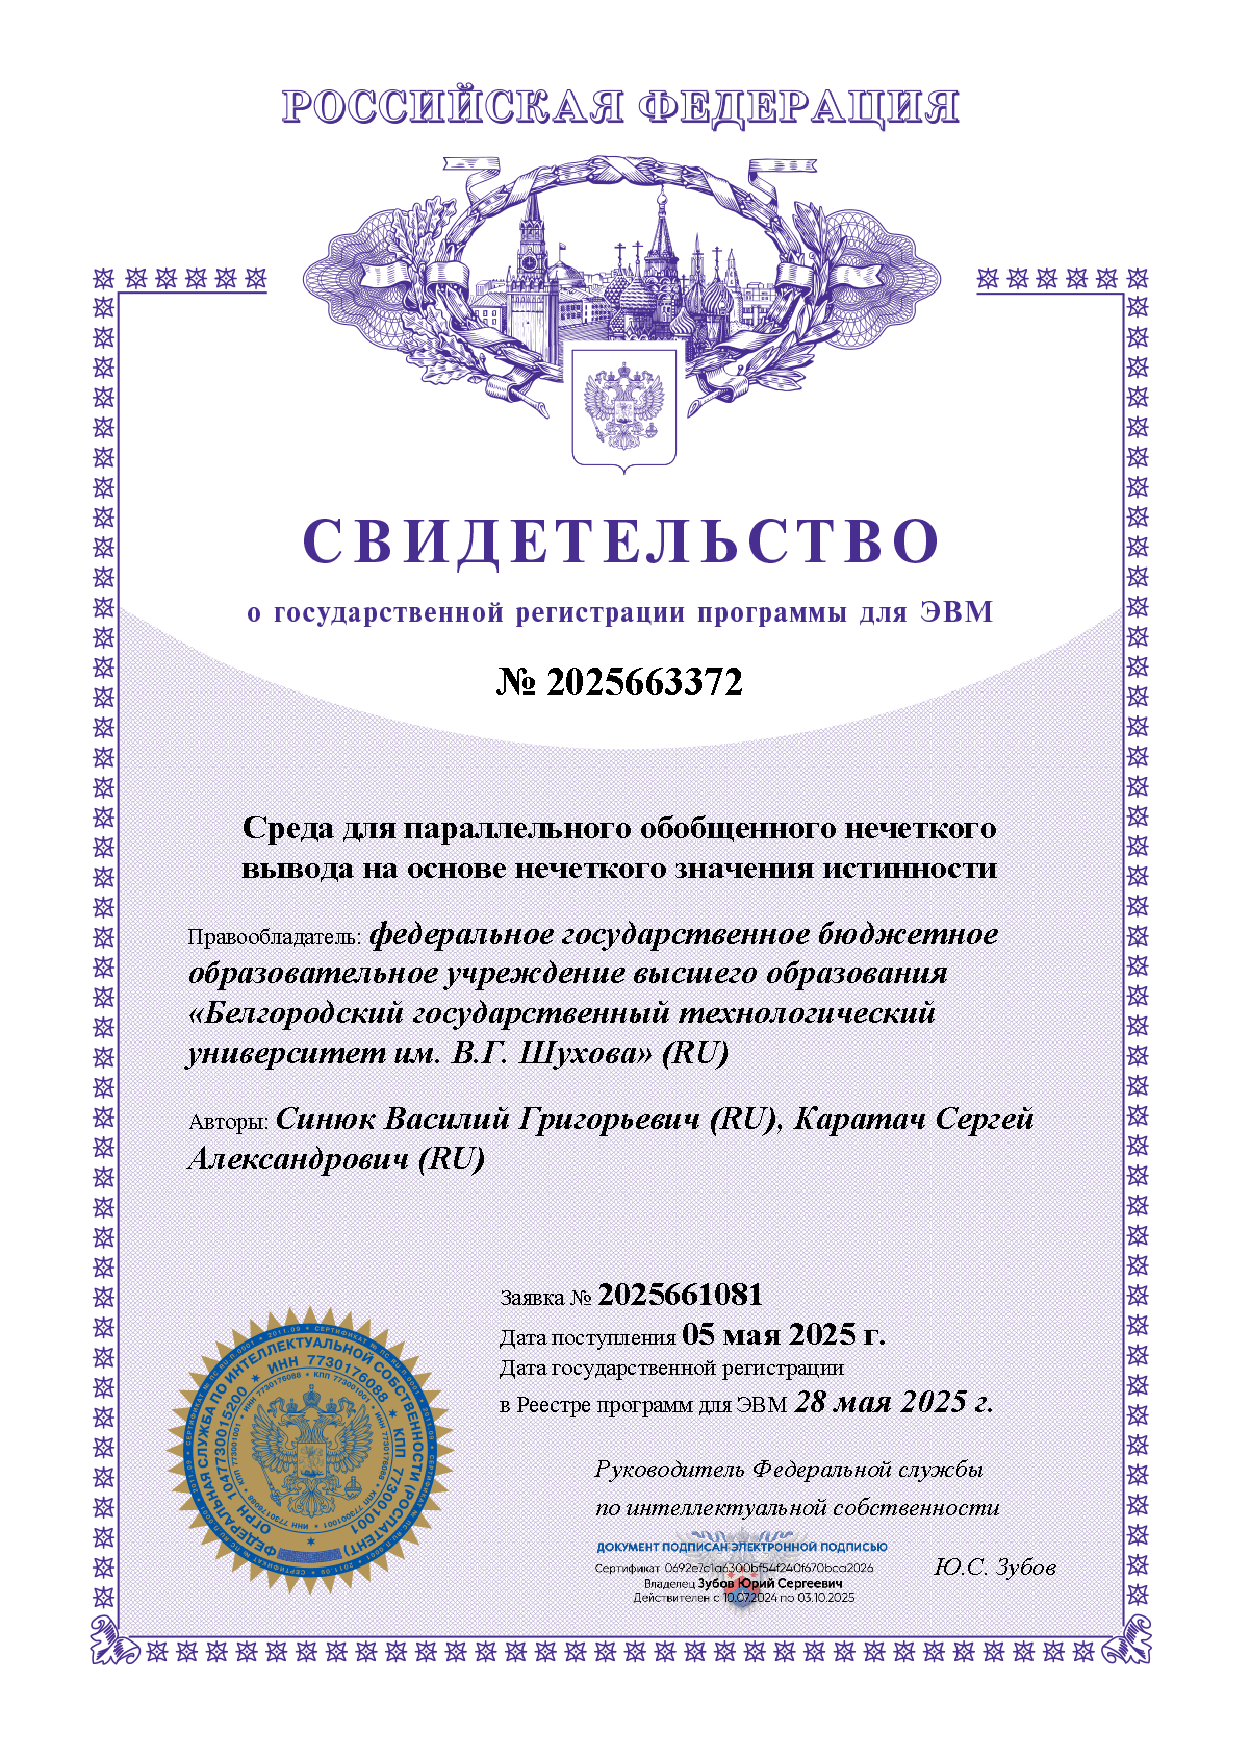
\includegraphics[width=0.9\textwidth, page=1]{images/RosPatent1.pdf}

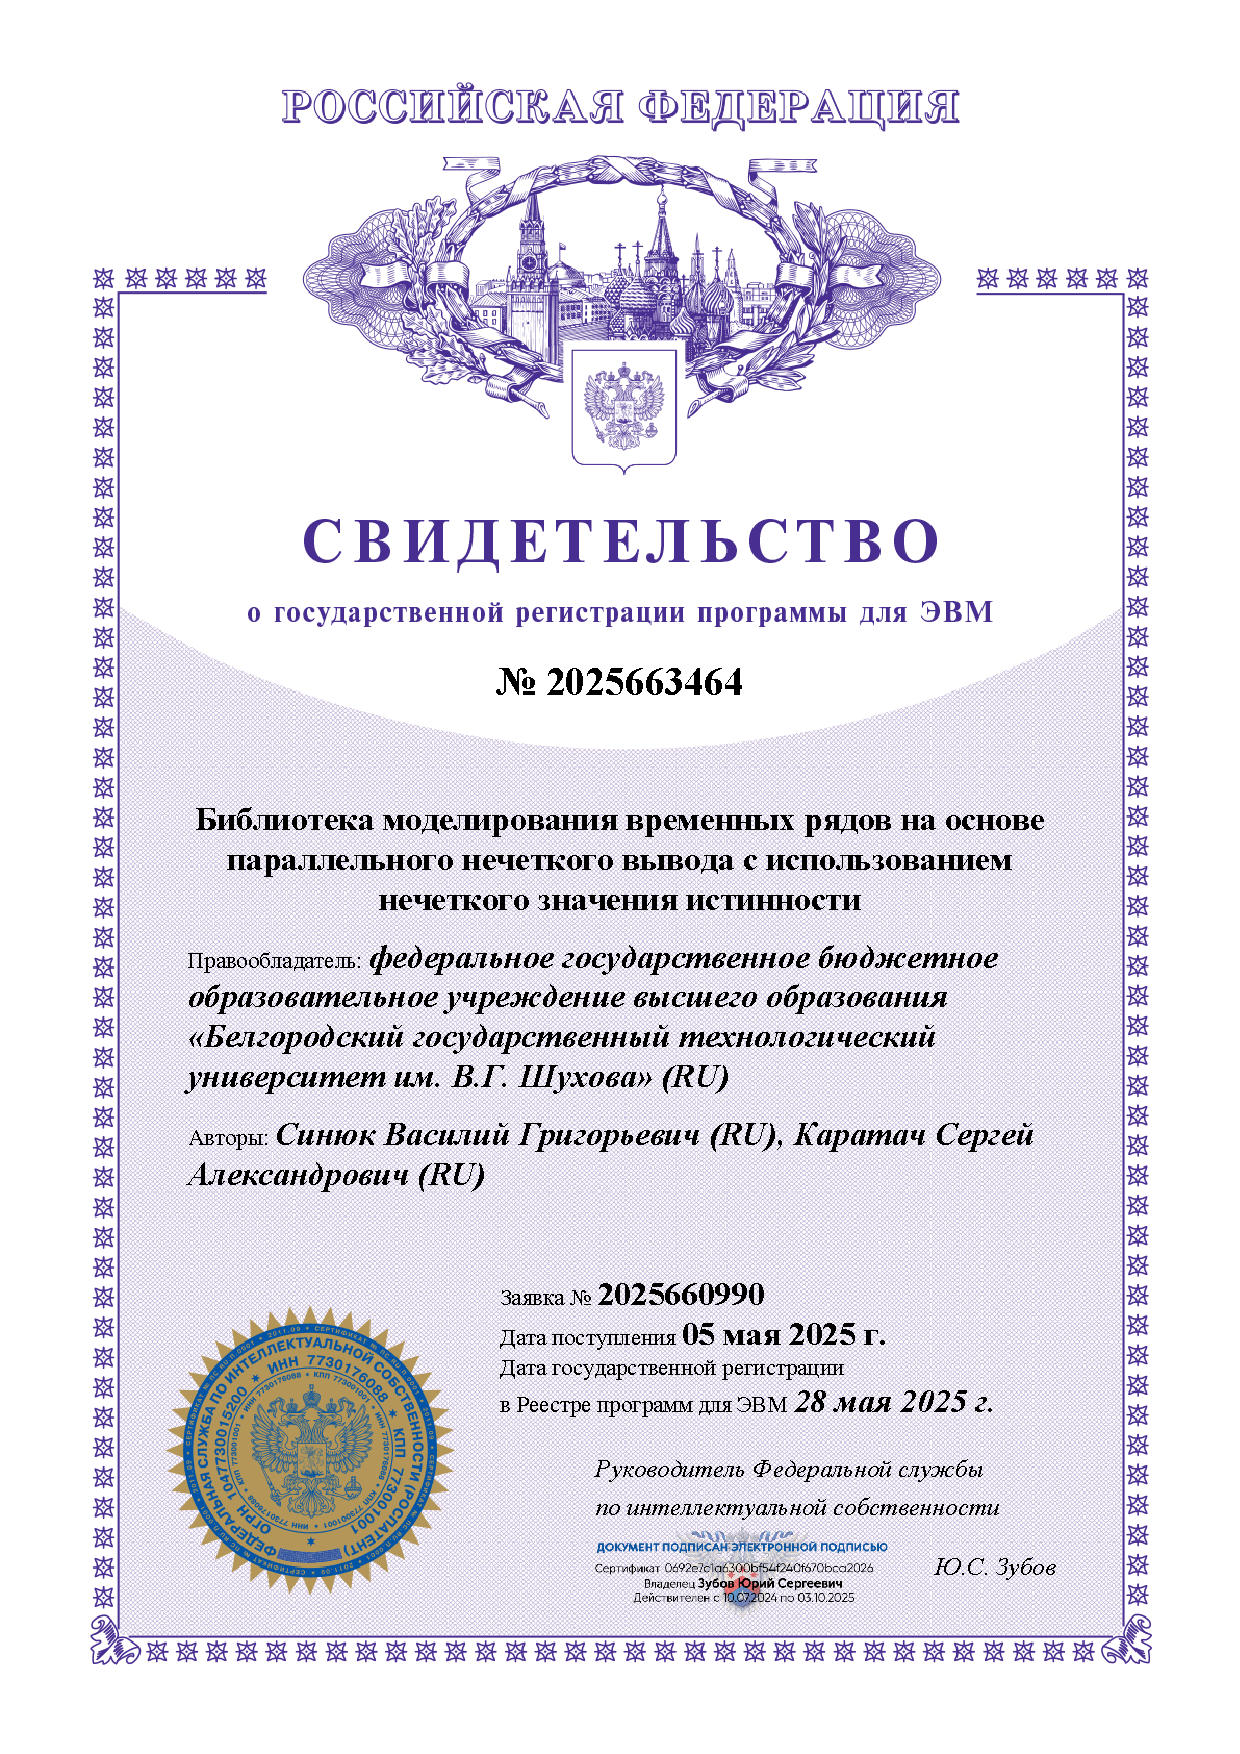
\includegraphics[width=0.9\textwidth, page=1]{images/RosPatent2.pdf}

%\chapter{Акт о внедрении результатов диссертационной работы в рабочий процесс}\label{app:C}

%\includepdf[pages=-]{images/act.pdf}
        % Приложения

\setcounter{totalappendix}{\value{chapter}} % Подсчёт количества приложений

\end{document}
